% **************************************************************************************************************
% A Classic Thesis Style
% An Homage to The Elements of Typographic Style
%
% Copyright (C) 2015 André Miede http://www.miede.de
%
% If you like the style then I would appreciate a postcard. My address 
% can be found in the file ClassicThesis.pdf. A collection of the 
% postcards I received so far is available online at 
% http://postcards.miede.de
%
% License:
% This program is free software; you can redistribute it and/or modify
% it under the terms of the GNU General Public License as published by
% the Free Software Foundation; either version 2 of the License, or
% (at your option) any later version.
%
% This program is distributed in the hope that it will be useful,
% but WITHOUT ANY WARRANTY; without even the implied warranty of
% MERCHANTABILITY or FITNESS FOR A PARTICULAR PURPOSE.  See the
% GNU General Public License for more details.
%
% You should have received a copy of the GNU General Public License
% along with this program; see the file COPYING.  If not, write to
% the Free Software Foundation, Inc., 59 Temple Place - Suite 330,
% Boston, MA 02111-1307, USA.
%
% **************************************************************************************************************
\RequirePackage{fix-cm} % fix some latex issues see: http://texdoc.net/texmf-dist/doc/latex/base/fixltx2e.pdf
\documentclass[ twoside,openright,titlepage,numbers=noenddot,headinclude,%1headlines,% letterpaper a4paper
                footinclude=true,cleardoublepage=empty,abstractoff, % <--- obsolete, remove (todo)
                BCOR=5mm,paper=a4,fontsize=11pt,%11pt,a4paper,%
                frenchb,english,%
                ]{scrreprt}

%
\chapter*{Avant-Propos}

\begin{flushright}{\slshape    
	Une civilisation sans la science \\
	c'est aussi absurde qu'un poisson sans bicyclette.} \\ \medskip 
	--- Pierre Desproges
\end{flushright}

\vspace{0.5cm}
%\begin{itemize}
%\item la révolution industrielle
%\item migration vers les villes (50\% de la population mondiale depuis pas longtemps)
%\item déconnexion de la terre a cause du béton
%\item déconnexion du ciel a cause des éclairages publique
%\item étudier l'astrophysique est essentiel pour que l'Homme reste humble et considère sa place dans l'univers pour ne pas courir a sa perte.
%\end{itemize}

La question de la place de l'Humanité dans l'Univers a toujours été centrale et au cœur des préoccupations de toutes les civilisations.
De nombreuses cosmologies ont vues le jours au fil des siècles et des peuples.

%Toutes ont en commun 

Il fut un temps ou l'Homme n'avait d'autre choix que de cultiver les champs le jour et vivre dans l'obscurité la nuit.
Il existait un lien fort entre ce qui se passait sur terre (Humanité vient de Humus après tout) et dans le ciel.
Il ne pouvait que constater le ciel étoilé et se poser la question de la provenance des lueurs qui remplissent la voûte céleste.

Absence de lumière a toujours créer une peur de l'inconnu, cette fameuse peur du noir.
Depuis le XIX ème siècle et la revolution industrielle, il est devenu possible de s'affranchir de la nuit.
Et nous ne nous en sommes pas privé.

Nous vivons dans un monde ou plus de la moitié de la population mondiale vie dans des villes ou l'obscurité n'a pas sa place.
L’éclairage publique agis comme un écran qui nous bloque la vue du ciel, et par la même occasion inhibe cette sensation de vertige que l'on peu ressentir en le regardant.

Cette migration urbaine à aussi pour conséquence de nous couper du lien a la terre
Les villes sont presque intégralement étanchéifiée par du béton.

L'étude de la cosmologie et sa vulgarisation est une nécessité si l'on veux retrouver une certaine humilité vis a vis de notre seul et unique lieu de vie.


\vspace{0.5cm}


\begin{flushright}{\slshape    
	You devellop an instant global consciousess, \\
	a people orientation,\\
	an intense dissatisfaction with the state of the world,\\
	and a compulsion to do something about it.\\
	From out there on the moon, internationnal politic look so petty. \\
	You want to grab a politician by the scuff of the neck\\
	and drag him a quarter of a million mile out and say: \\
	'Look at that you son of a bitch'\\ \medskip 
	--- Edgar Mitchell Appolo 14 astronaut }
\end{flushright}
%\chapter{Introduction}
%Besoin des simu car contraintes observationnelles sur IGM mais impact fort sur les galaxies, pas le même timing, physique complexe il faut simulaer
%
%D'une manière générale, la méthode scientifique repose sur 3 piliers: 
%\begin{enumerate}
%\item L'observation
%\item La théorie
%\item L'expérience
%\end{enumerate}
%L'astrophysique moderne n’échappe pas à cette règle.
%
%\paragraph{L'observation} est le plus ancien des piliers, et constitue le point de départ de toute démarche scientifique.
%L'Homme a toujours regardé le ciel, et avant même de chercher à le comprendre, il a recueilli des informations à son sujet. %le regarder et l'analyser.
%Contrairement aux autres discipline scientifique, le point de vue que nous avons sur notre sujet d'analyse est unique, il nous est impossible d'observer l'Univers sous un autre angle.
%%Les techniques d'observations ont fait d’énormes progrès ces dernières années, mais observer ne suffit pas.
%
%%Il celui sur lequel repose le plus de poids puisque tout en découle.
%%De plus il est commun a toute les disciplines scientifique.
%%Il n'est pas de science possible sans observation.
%
%\paragraph{La théorie} est le deuxième piliers.
%%Lorsque l'on voit ces lumière sur la voûte céleste, nous sommes obligé de nous poser la question essentielle de leur provenance.
%%Cette question mène a l'élaboration de diverse formulation tentant d'expliquer comment (et pourquoi) le ciel s'illumine la nuit.  
%%Dans le cadre de l'étude de l'univers dans sont ensemble, cette théorie est nommée cosmologie et repose sur des concept mathématiques complexes
%L'objectif est ensuite de réussir à donner un sens aux informations récoltées et de prédire les prochaines observations.
%%Au fil des siècles, diverses théories ont été élaborées pour expliquer le comportement de l'Univers observable.
%En effet, la force d'une théorie est jugée à sa capacité à faire des prédictions.
%%A partir de la théorie, on réalise un modèle, un ensemble de règles  permettant de définir l'évolution d'un système connaissant son état actuel.
%
%\paragraph{L'expérience} est le dernier pilier.
%D'une manière générale, l'expérience a pour but de mettre a l’épreuve la théorie, et représente un ensemble d'actions, réalisées en suivant un protocole, permettant d'obtenir des résultats reproductibles.
%A l'inverse d'autres domaines scientifique, en astrophysique notre portée d'interaction est réduite.
%Il ne nous est ni possible d'effectuer des expériences sur l'Univers, ni de changer notre point d'observation.
%Les simulations numériques permettent de palier à ces problèmes en créant virtuellement des portions d'espace respectant un certain modèle.
%Un modèle, étant un ensemble de règles, issues de la théorie et permettant de définir l'évolution d'un système en connaissant son état actuel.
%%Pilier le plus récent il est sensé palier au problème des deux autres : l'impossibilité de changer de point de vue ou de tester les théories élaborées.
%%Ici sous entendue la simulation numérique, il est beaucoup plus récente et dépend grandement de la technologie.
%%C'est celui vers lequel j'ai choisis de me diriger.
%
%%observation, modélisation et test de la théorie or en astro on ne peut pas tester directement donc on simule.
%
%\paragraph{}
%
%Cette thèse est articulée principalement autour du dernier pilier.
%Une grande partie de cette thèse a été consacrée à l'élaboration d'un modèle numérique dédié à l'étude de la réionisation.
%Puis, dans le but d'explorer ce modèle, un nombre important d'expériences (de simulations) ont été réalisées.
%Dans cette première partie, je vais introduire quelques grands concepts liés a l'étude numérique de la réionisation, puis je présenterai la structure du présent manuscrit en m'appuyant sur ces concepts.
%
%\subsection*{Le modèle standard}

Notre compréhension actuelle de l'Univers s'inscrit dans le cadre du modèle standard de la cosmologie.
Ce modèle repose sur un Univers non statique et en expansion, ayant une origine, le Big-Bang.
Très tôt dans son évolution, l'Univers était extrêmement chaud et dense, il n'y avait alors ni étoiles ni galaxies.
Après l'émmission du fond diffus cosmologique 380000 ans Big-Bang, l'Univers était froid et majoritairement composé de gaz neutre.
%Mais sous l'effet de l'expansion, le plasma primordial s'est refroidi, les premiers atomes se sont formés lors de ce que l'on nomme la recombinaison, qui a mené à l'émission du fond diffus cosmologique.
%L'Univers était alors extrêmement homogène que ce soit en densité ou en température, mais cette homogénéité n'était pas parfaite.
%S'en suit une période où les in-homogénéités primordiales se sont effondrées sur elles même du fait de la gravité.
%Puis, environ trois cents millions d'années après le Big-bang ces in-homogénéités sont devenues suffisamment denses pour former les première étoiles.
%Ces étoiles ont émis un rayonnement suffisamment énergétique pour séparer les électrons et les protons liés au moment de la recombinaison.
%L'univers c'est alors retrouvé une nouvelle fois dans un état majoritairement ionisé : c'est ce que l'on nomme la réionisation.
%\subsection*{La réionisation}
%La réionisation constitue le dernier grand changement que l'univers ai subit lorsqu'il était âgé de moins d'un milliard d'années.
L'effondrement gravitationnel du gaz qui a permit par endroits une élévation de densité et de température suffisante pour réamorcer des réactions de fusion thermonucléaire est à l'origine de la formation des premières générations d'étoiles,
%Il s'agit de la première génération d'étoiles.
%Le matériaux disponible pour leurs formations était alors abondant.
%On pense que ces étoiles étaient beaucoup plus massives, et donc beaucoup plus énergétique que les étoiles observées actuellement.
%Cette première génération 
qui ont émis un rayonnement ultraviolet ionisant qui a grandement impacté le milieu environnant : c'est cette étape que l'on nomme la réionisation.%, en le chauffant et en l'ionisant. % par effet thermique et en le déplaçant par effet de pression de radiation.
La réionisation n'est pas un processus instantané, et il est estimé aujourd'hui que les premières étoiles sont apparues alors que l'Univers était âgé d'environ 300 millions d'années. 
Il fallut alors 700 millions d'années supplémentaires pour que le rayonnement remplisse l'Univers, situant ainsi la fin de la période de réionisation à environ un milliard d'années après le Big-bang.

%
%De plus, à la fin de leur vie, ces étoiles massives ont explosé en supernovæ, effectuant alors un puissant chauffage ainsi qu'un fort brassage du gaz.
%En changeant la configuration du milieu, ces premières étoiles ont modelées les lieux d'apparition des générations suivantes et par effet de cascade a eu un impact sur la distribution de matière observée aujourd'hui.
%
%%La vitesse de la lumière étant finie, il fallut un certain temps pour que les premiers rayons ionisant puisse atteindre tous les recoins de l'Univers. 
%
%%C'est cette transition entre un univers neutre et froid vers un univers chaud et ionisé que l'on appel l'époque de réionisation.
%%L'apparition des première sources lumineuse a eu un impact sur la façon dont la matière c'est organisée pour former les galaxies.
%%Il est probable que l'univers que l'on observe aujourd'hui, ai conservé les traces de cette grande époque de transition.
%
%Une des difficulté à l'étude de la réionisation est l'époque à laquelle elle s'est produite. %on considère actuellement qu'elle a eu lieu dans le premier milliard d'année de l'univers.
%Pour observer l'Univers jeune, il faut regarder loin, et les meilleurs télescopes actuels ne sont pas encore assez performants pour atteindre des époques aussi lointaines.
%Il faudra attendre encore au moins une décennie avant la mise en place des prochaines générations de télescopes assez puissants pour observer les environnements de formation de ces premières sources lumineuses.
%
%\subsection*{Les simulations numériques}
%
%Les premières simulations cosmologiques ne considéraient l'évolution que de la matière noire. %la composante non collisionnelle de la matière, ie .
%Comme celle ci constitue la masse la plus abondante de l'Univers, ces simulations permettent de suivre l'évolution de la distribution de matière sur les grandes échelles. 
%Mais comme la matière noire est invisible, il manquait une composante importante : les baryons.
%Lorsque l'intérêt fut porté sur la formation des galaxies, le calcul de l'hydrodynamique du gaz fut alors introduit, puis avec lui les premiers modèles de formation stellaire apparurent.
%Mais la communauté a vite été confrontée a un important problème: le gaz refroidissait trop.
%Ce qui menait à une formation d'étoile trop abondante car rien n’empochait le gaz de s’effondrer sur lui même.
%Pour palier à ce problème, il fut proposé d'injecter de l'énergie dans les endroits les plus denses.
%Cette énergie, introduite par les supernovæ, permet de chauffer le gaz et ralenti son effondrement. 
%%Depuis très récemment, une troisième physique est devenue  dans les simulations l'influence de la radiation sur le milieu est également prise en compte.
%Aujourd'hui, l'intérêt est porté sur l'introduction d'une nouvelle physique, celle du rayonnement.
%Le rayonnement émit par les étoiles, va changer les propriétés physico-chimique et thermique du gaz qui les environnent et ainsi modeler les lieux d'apparitions des générations futures d'étoiles.
%
%Même si les possibilités d'observations sont restreintes, nous pouvons utiliser les simulations numériques pour tenter de comprendre les phénomènes en cours à cette époque.
%En effet, les phénomènes en action pendant la réionisation sont nombreux et les modèles analytique trouvent leurs limites.
%Avec l'avancée exponentielle des capacités de calculs, les ordinateurs se transforme petits a petit en véritable laboratoire pour les astrophysiciens.


\paragraph{}
Voici un aperçu de ces questions que nous allons aborder dans cette thèse: 

\begin{itemize}
\item Quelles sont les physiques nécessaires à la bonne modélisation de l'époque de la réionisation ?
\item À quelles échelles ces phénomènes interviennent t il ?
\item Comme la formation stellaire des premières générations d'étoiles à impactée l'apparition des générations suivantes ? %le déroulement de la réionisation ?
\item Quel impact la réionisation a elle eu sur la formation des galaxies ?
\item Comment s'est propagée l'ionisation dans l'Univers ?
\item Y a t-il des marques de la réionisation dans l'Univers local ?
\item L'Univers a t-il été réionisé par quelques grosses sources très lumineuses ou par de nombreuses sources moins énergétiques ?
\end{itemize}

Pour étudier des phénomènes aussi fortement couplés que ceux considérés dans le cas de l'époque de réionisation, il est nécessaire d'avoir recours à des simulations numériques. 
%Le but de ces simulations est de reproduire les observations sur la distribution de matière dans l'Univers.
A l'heure actuelle, il commence à être possible de simuler de manière auto cohérente, l'effondrement de structures cosmologiques, contenant du gaz, formant des étoiles, qui émettent du rayonnement.
%Ces simulations ont pour objectif d'aider à comprendre quelques unes des grandes questions en suspend dans l'étude de la réionisation.
Mais l'utilisation de simulation introduit également quelques question : 

\begin{itemize}
\item Comment simuler la réionisation efficacement ?
\item Comment modéliser au mieux les différents physiques à l’œuvre ?
\item De quelle résolution à t-on besoin ?
\item Comment tirer profit au maximum du matériel disponible ?
\item Quels sont les compromis nécessaire ?
\end{itemize}

%\begin{itemize}
%\item Quand sont apparues les premières sources lumineuses?
%Nous verrons que les observations imposent certaines contraintes sur la fin de la réionisation mais nous n'avons actuellement que très peu de contraintes sur la durée du processus.
%
%\item L'Univers a t-il été réionisé par quelques grosses sources très lumineuses ou par de nombreuses sources moins énergétiques ?
%La question reste ouverte de savoir si se sont les quasars, sources relativement rares mais pouvant être extrêmement énergétiques, ou les galaxies plus modestes mais beaucoup plus nombreuses?
%Dans le cas où se serait les galaxies, serait-ce les plus légères, extrêmement nombreuses ou les plus massives?
%
%\item Comment ces premières générations d'étoiles ont influencées l'apparition des suivante, et ont elles laissées des traces encore visibles dans l'environnement proche?
%
%\end{itemize} 

%En répondant à certaines de ces questions, les simulations numériques permettent de mieux cibler les futures missions d'observations, et augmentent les chances de réussites.

%En étudiant au préalable ce que l'on cherche à observer, on a plus de chance d'observer au bon endroit et de la bonne facon.

%Au stade actuel de notre compréhension de l'univers, les simulations numériques ont a la fois de très belles réussites mais souffres également de 

%\subsection*{Le groupe local}
%Le groupe local est un ensemble de quelques dizaines de galaxies, dont les principales représentantes sont la Voie Lactée et notre voisine Andromède.
%Il s'agit de notre environnement galactique proche.
%Ce qui le rend facilement observable.
%L'observation de cet environnement nous fournis des informations essentielles sur la cosmologie de l'Univers.
%
%Plus la precision des observations augmente, plus il est nécessaire d'avoir des simulations résolues disposant de toutes la physique nécessaire pur expliquer globalement les échelles considérées.
%Les premières simulations de matière noires ont permit d'expliquer les observations réalisées sur la distribution de la matière aux grandes échelles.
%Lorsque les capacité de calcul se sont révélées suffisantes pour explorer des résolutions plus fines, il est vite apparu un certain décalage entre simulation et observation. 
%L'introduction de l'hydrodynamique a permis d'augmenter l'accord entre les deux, jusqu'à un second palier de résolution.
%Aujourd'hui, l'introduction de la physique du rayonnement va certainement permette de diminuer encore les échelles auxquelles les simulations sont sont en accord avec les observations.
%L'ordre de grandeur de ces échelles est celui de la taille du groupe local.
%
%De plus, les échelles que l'on considère dans les simulations cosmologiques a rayonnement couplé se rapproche de plus en plus des échelles considérés dans les simulations d'évolution de galaxies.
%L'objectif est ici de faire le lien entre la physique de l'univers dans son ensemble (la cosmologie) et de la physique régissant l'évolution de notre galaxie ou de sa voisine (la physique galactique).


\section{Mes travaux}

Dans l'objectif de répondre à certaine de ces questions, il est nécessaire de développer des outils.
EMMA, un code de simulations cosmologiques dédié à l'étude de la réionisation, à été mon principal outil durant cette thèse.
J'y ai apporté différentes contributions, allant de l'ajout de nouvelles fonctionnalités jusqu'à la simple résolution de conflits, en passant par l'optimisation de certaine parties.

Une de mes principales contributions a été l'implémentation d'un modèle de formation et d'évolution stellaire et une étape importante de cette thèse a été sa calibration..
Ce modèle dispose de plusieurs paramètres libres, et leurs valeurs étant directement fonction de la résolution, il a naturellement été choisi d'utiliser la résolution des plus grosse simulations à l'heure actuelle.
Cette calibration a été une étape préliminaire à la réalisation de la simulation CODA I-AMR une des plus grosse simulation de la réionisation à l'heure actuelle.
% une simulation représentant un volume de $(100 cMpc)^3$ échantillonné par $2048^3$ éléments de résolutions et une résolution adaptative allant jusqu'à 500pc.
%Les ressources de calculs étant limitées, il est nécessaire de faire certaines concessions, le choix doit être fait entre volume physique et résolution.
Les ressources de calculs étant limitées, il n'est pas possible de réaliser plusieurs de ces simulations.
Or la calibration nécessite un grand nombre de tests, j'ai pour cella exécuté des simulations de taille réduite à $(12 cMpc)^3$ avec une résolution comparable à celle de la simulation CoDa I AMR. 
L'objectif est d'explorer une partie de l'espace de paramètres du modèle, et de comprendre, sur des échantillons, quel est l'influence des paramètres libres sur les résultats obtenus, et leur interprétation dans des simulations plus grandes.

%Pour analyser les nombreuse simulations obtenues dans de bonnes conditions, j'ai développé une librairie pour d'analyse et la gestion des données.
%Cette librairie rassemble une grandes part des outils d’analyse que j'ai développé et est en accès libre, pour faciliter l'accès d'EMMA à ses nouveaux utilisateurs.
%visu

Dans l'objectif de diminuer les concessions à réaliser sur la taille et la résolution des simulations, il existe différentes pistes : soit augmenter l'accès aux ressources de calculs, soit optimiser les codes de simulations.
Un des mes objectif a été de mieux cerner l'ensemble des techniques utilisées dans un tel code pour être en mesure de cibler au mieux les points à améliorer.

Il existe entre autre une technique consistant à diminuer numériquement la vitesse de la lumière pour réduire artificiellement, la charge de calcul.
Je me suis posé la question du domaine de validité de cette approximation, et du gain maximum que l'on peut espérer grâce à cette technique tout en restant dans un domaine d'approximation raisonnable.

%\textit{Quels sont les facteurs qui limitent la performance globale de EMMA et comment les améliorer?}
%
%Une autre piste n'est pas algorithmique mais matérielle.
%L'utilisation de processeurs graphique permet dans certain cas des accélération considérable (jusqu’à deux ordre de grandeurs).
%Cependant l'utilisation de ce matériel impose certaines précaution et si une grande partie d'EMMA l'utilise déjà, le potentiel d'accélération reste grand.


\section{Organisation du manuscrit}
%\begin{itemize}
%\item Introduction au   cosmologique $\Lambda$ CDM et a la période de réionisation.
%\item Présentation du model numérique (Papier emma)
%\item Présentation du model d'étoiles (papier SN)
%\item Présentation de l'outils des cartes de reionization (papier c)
%\item 
%\end{itemize}

Ce manuscrit est articulé autour de différents travaux auxquels j'ai contribué durant ma thèse.
Après le présent chapitre introductif, la première partie sera consacrée à la mise en place du contexte.
Une fois les grandes lignes du modèle physique introduites, et le contexte de la réionisation posé, j'aborderai plus spécifiquement mes travaux.
Je m'appuierai sur chacune des publications auxquelles j'ai contribué, et articulerai un chapitre autour de chacune d'elles. 

\paragraph{Contexte :}
Le chapitre \ref{ch:introduction_physique} constitue une introduction aux concepts utiles en cosmologie.
Ces concepts seront nécessaires pour aborder le chapitre \ref{sec:introreio} qui explore plus spécifiquement la période de réionisation.

\paragraph{Méthodes numériques :}
Une partie sera consacrée à EMMA l'outil central de cette thèse.
%, un code capable de simuler l'évolution de la matière noire, du gaz et de la radiation à des échelles cosmologiques de manière entièrement couplé, et ayant pour principal objectif l'étude de la période de réionisation.
Dans le chapitre \ref{ch:introduction}, je commencerai par présenter les grandes lignes de \emma, et introduirai sa maille adaptative qui contraindra plusieurs choix par la suite.
Le chapitre \ref{sec:solvers} sera consacré au développement des différents moteurs physiques et de leurs concepts numériques associés.
Puis dans le chapitre \ref{sec:materiel}, l'accent sera mis sur les techniques de parallélisation utilisées dans EMMA qui a la particularité d'être massivement parallèle et d'être accéléré par processeurs graphiques.
Cette approche permettra au lecteur de mieux appréhender les résultats obtenus à partir des simulations générées ensuite avec ce code.

\paragraph{Modèle stellaire :}
Comme l'étude du rayonnement émis dans l'Univers passe immanquablement par l'étude de la formation stellaire, je consacrerai le chapitre \ref{sec:etoiles} à détailler le modèle de formation et d'évolution stellaire de EMMA, ainsi que ses contraintes, ses limites, et les différents tests qui ont été exécutés pour sa calibration.
Je présenterai ensuite dans le chapitre \ref{sec:galaxies} une étude que j'ai menée à l'aide de ce modèle, visant à mieux comprendre la physique à l'œuvre dans les grandes simulations de la réionisation.
L'objectif est de comprendre quelles sont les galaxies qui contribuent à la réionisation dans nos modèles et quel est l'impact du feedback stellaire sur cette contribution.

\paragraph{Cartes de réionisation :}
Le chapitre \ref{sec:intre:zreio} sera consacré à une étude sur l'influence de l'approximation de la vitesse de la lumière réduite sur la propagation des fronts d'ionisation.
Nous verrons que dans les simulations de la réionisation, la vitesse de la lumière peut être changée de manière à économiser du temps de calcul.
J'ai cherché a quantifier dans quelle mesure celle ci peux être réduite avant que cela ai un impact sur les résultats des simulations.
Pour cela j'ai développé un méthode pour calculer la vitesse des fronts d'ionisation, en utilisant les cartes de réionisation, outils qui sera également introduit dans cette partie.

Le chapitre \ref{sec:CODAEMMA} sera dédié à la présentation de la simulation "CoDa II AMR". %, une des plus grosse simulation de la réionisation à l'heure actuelle.
J'y présenterai les premiers résultats obtenus à propos du liens entre la masse des halos contenus dans la simulation aujourd'hui et leurs histoires au moment de la réionisation.
Cette étude sera menée à l'aide des cartes de réionisation.

\paragraph{Visualisation : }
Nous verrons ensuite un court chapitre  \ref{sec:visu}, consacré à la présentation de travaux liés à la visualisation des simulations cosmologiques.
J'y aborderai différentes méthodes de visualisations ainsi que quelques détails technique liés à leurs implémentations.

%Ce modèle constitue une de mes principale contributions à \emma.
%J'ai implémenté dans \emma, un modèle de transformation du gaz en particule stellaire.
%Ce modèle se base sur un critère de densité pour 
%Lorsque, sous l'effet de la gravitation, une cellule devient suffisamment dense, celle ci devient autorisée à former des étoiles.
%Toute les cellules autorisées vont alors transformer une certaine quantité du gaz en particule stellaire, en fonction de l'état local de la cellule, et suivant une loi empirique issue de l'observation : la loi de Schmidt-Kennicutt.
%Les particules nouvellement créées vont alors émettre du rayonnement ionisant pendant un certain temps.
%A la fin de leurs vie, ces particules stellaires vont exploser en supernovæ, injectant ainsi une quantité non négligeable d'énergie dans le milieu environnant.
%Cette énergie supplémentaire perturbe le milieu et régule la formation stellaire.
%J'ai implémenté différents modèles d'injection d'énergie dans le solveur hydrodynamique d'\emma{ } et comparé ces modèles entre eux. 

%Comme ces modèles nécessite l'introduction de plusieurs paramètres libres, une partie importante du temps a été consacrée à l'exploration et à la calibration de ces paramètres.


%Ce modèle considère deux types d'énergie. 
%La première, thermique, va dissiper une certaine partie de l'énergie disponible dans le chauffage du gaz.
%La seconde, cinétique, va mettre en mouvement le gaz environnant avec le reste de l'énergie.
%Une certaine proportion de la masse de la particule stellaire est retournée dans le milieu. 
%L'énergie totale et la masse des éjectas étant contrainte par un autre modèle, Starburst99.



%J'ai contribué à différents aspects du code mais une de mes 
%Au moment de mon arrivé en thèse,
%D'une manière plus générale j'ai contribué à divers aspect du code, comme la gestion des paramètres utilisateur, l'écriture des données de sorties ou encore la documentation.
%Dans la première partie de ma thèse, ma tache principale a été d'implémenter un scénario de formation stellaire, ainsi qu'un modèle de feedback de supernovae.
%Je développe également une librairie d'analyse des fichiers générés par \emma.


%J'ai également contribué au développement d'un code de visualisation et d'exploration de simulations astrophysique.


%
%\subsection*{Mod\`ele de formation stellaire}

%
%\subsection*{Mod\`ele de supernovae}
%
%Historiquement, les modèles de formation stellaire se sont rapidement confronté à un problème majeur : ils n'arrivaient pas à reproduire les observations en terme de quantité d'étoiles crées.
%Une réponse à ce problème fut l'introduction des supernovaes. 

%
%De la même manière que précédemment, l'implémentation de ce modèle a introduit plusieurs paramètres libres qu'ils a fallut calibrer.
%
%A partir de ce modèle numérique j'ai ensuite réalisé plusieurs études:
%
%\begin{itemize}
%\item en faisant varier le modèle de feedback stellaire j'ai tenté de quantifier son influence sur le déroulement du processus de réionisation.
%\item J'ai étudié la vitesse de propagation des fronts d'ionisations et montré que le reionisation s'éffectue en 2 phases. 
%\item Le develloppement de ce modèle a conduit a la réalisation de l'une des plus grosses simulations de la réionisation a l'heure actuelle la simulation CODA-EMMA.
%J'introduirais cette simulation ainsi que les premiers résultats obtenus.
%\item Enfin, je présenterai mes travaux concernant la visualisation de données de simulations.
%\end{itemize}
%


%\includeonly{Chapters/part_01/CDM}
%\includeonly{Chapters/part_01/reionization}

%\includeonly{Chapters/part_02/EMMA}
%\includeonly{Chapters/part_02/solver}
%\includeonly{Chapters/part_02/materiel}

%\includeonly{Chapters/part_03/etoiles}
%\includeonly{Chapters/part_03/halos}
%\includeonly{Chapters/part_03/supernovae}

%\includeonly{Chapters/Chapter04_Carte_reio}

%\includeonly{Chapters/Chapter05_z0}

%\includeonly{Chapters/part_06/visualisation}


%********************************************************************
% Note: Make all your adjustments in here
%*******************************************************
% ****************************************************************************************************
% classicthesis-config.tex 
% formerly known as loadpackages.sty, classicthesis-ldpkg.sty, and classicthesis-preamble.sty 
% Use it at the beginning of your ClassicThesis.tex, or as a LaTeX Preamble 
% in your ClassicThesis.{tex,lyx} with % ****************************************************************************************************
% classicthesis-config.tex 
% formerly known as loadpackages.sty, classicthesis-ldpkg.sty, and classicthesis-preamble.sty 
% Use it at the beginning of your ClassicThesis.tex, or as a LaTeX Preamble 
% in your ClassicThesis.{tex,lyx} with % ****************************************************************************************************
% classicthesis-config.tex 
% formerly known as loadpackages.sty, classicthesis-ldpkg.sty, and classicthesis-preamble.sty 
% Use it at the beginning of your ClassicThesis.tex, or as a LaTeX Preamble 
% in your ClassicThesis.{tex,lyx} with \input{classicthesis-config}
% ****************************************************************************************************  
% If you like the classicthesis, then I would appreciate a postcard. 
% My address can be found in the file ClassicThesis.pdf. A collection 
% of the postcards I received so far is available online at 
% http://postcards.miede.de
% ****************************************************************************************************


% ****************************************************************************************************
% 0. Set the encoding of your files. UTF-8 is the only sensible encoding nowadays. If you can't read
% äöüßáéçèê∂åëæƒÏ€ then change the encoding setting in your editor, not the line below. If your editor
% does not support utf8 use another editor!
% ****************************************************************************************************
\PassOptionsToPackage{utf8}{inputenc}
	\usepackage{inputenc}

% ****************************************************************************************************
% 1. Configure classicthesis for your needs here, e.g., remove "drafting" below 
% in order to deactivate the time-stamp on the pages
% ****************************************************************************************************
\PassOptionsToPackage{eulerchapternumbers,listings,drafting,%
					 pdfspacing,%floatperchapter,%linedheaders,%
					 subfig,beramono,eulermath,parts}{classicthesis}                                        
% ********************************************************************
% Available options for classicthesis.sty 
% (see ClassicThesis.pdf for more information):
% drafting
% parts nochapters linedheaders
% eulerchapternumbers beramono eulermath pdfspacing minionprospacing
% tocaligned dottedtoc manychapters
% listings floatperchapter subfig
% ********************************************************************


% ****************************************************************************************************
% 2. Personal data and user ad-hoc commands
% ****************************************************************************************************
\newcommand{\myTitle}{Simuler l'époque de reionization\xspace}
\newcommand{\mySubtitle}{Application au groupe local\xspace}
\newcommand{\myDegree}{Doctor (Dr.)\xspace}
\newcommand{\myName}{Nicolas Deparis\xspace}
\newcommand{\myProf}{Put name here\xspace}
\newcommand{\myOtherProf}{Put name here\xspace}
\newcommand{\mySupervisor}{Put name here\xspace}
\newcommand{\myFaculty}{Put data here\xspace}
\newcommand{\myDepartment}{Put data here\xspace}
\newcommand{\myUni}{Put data here\xspace}
\newcommand{\myLocation}{Strasbourg}
\newcommand{\myTime}{Decembre 2017\xspace}
\newcommand{\myVersion}{version 4.2\xspace}

% ********************************************************************
% Setup, finetuning, and useful commands
% ********************************************************************
\newcounter{dummy} % necessary for correct hyperlinks (to index, bib, etc.)
\newlength{\abcd} % for ab..z string length calculation
\providecommand{\mLyX}{L\kern-.1667em\lower.25em\hbox{Y}\kern-.125emX\@}
\newcommand{\ie}{i.\,e.}
\newcommand{\Ie}{I.\,e.}
\newcommand{\eg}{e.\,g.}
\newcommand{\Eg}{E.\,g.} 
% ****************************************************************************************************


% ****************************************************************************************************
% 3. Loading some handy packages
% ****************************************************************************************************

% ******************************************************************** 
% My packages
% ******************************************************************** 
\usepackage[dvipsnames]{xcolor}
\usepackage{pdfpages}


% ******************************************************************** 
% Packages with options that might require adjustments
% ******************************************************************** 
\PassOptionsToPackage{french,english}{babel}   % change this to your language(s)
% Spanish languages need extra options in order to work with this template
%\PassOptionsToPackage{spanish,es-lcroman}{babel}
	\usepackage{babel}                  

\usepackage{csquotes}
\PassOptionsToPackage{%
    %backend=biber, %instead of bibtex
	backend=bibtex8,bibencoding=ascii,%
	language=auto,%
	%style=numeric-comp,%
    style=authoryear-comp, % Author 1999, 2010
    %bibstyle=authoryear,dashed=false, % dashed: substitute rep. author with ---
    sorting=nyt, % name, year, title
    maxbibnames=10, % default: 3, et al.
    %backref=true,%
    natbib=true % natbib compatibility mode (\citep and \citet still work)
}{biblatex}
    \usepackage{biblatex}

\PassOptionsToPackage{fleqn}{amsmath}       % math environments and more by the AMS 
    \usepackage{amsmath}

% ******************************************************************** 
% General useful packages
% ******************************************************************** 
\PassOptionsToPackage{T1}{fontenc} % T2A for cyrillics
    \usepackage{fontenc}     
\usepackage{textcomp} % fix warning with missing font shapes
\usepackage{scrhack} % fix warnings when using KOMA with listings package          
\usepackage{xspace} % to get the spacing after macros right  
\usepackage{mparhack} % get marginpar right
%\usepackage{fixltx2e} % fixes some LaTeX stuff --> since 2015 in the LaTeX kernel (see below)
%\usepackage[latest]{latexrelease} % will be used once available in more distributions (ISSUE #107)
\PassOptionsToPackage{printonlyused,smaller}{acronym} 
    \usepackage{acronym} % nice macros for handling all acronyms in the thesis
    %\renewcommand{\bflabel}[1]{{#1}\hfill} % fix the list of acronyms --> no longer working
    %\renewcommand*{\acsfont}[1]{\textsc{#1}} 
    \renewcommand*{\aclabelfont}[1]{\acsfont{#1}}
% ****************************************************************************************************




% ****************************************************************************************************
% 4. Setup floats: tables, (sub)figures, and captions
% ****************************************************************************************************
\usepackage{tabularx} % better tables
    \setlength{\extrarowheight}{3pt} % increase table row height
\newcommand{\tableheadline}[1]{\multicolumn{1}{c}{\spacedlowsmallcaps{#1}}}
\newcommand{\myfloatalign}{\centering} % to be used with each float for alignment
\usepackage{caption}
% Thanks to cgnieder and Claus Lahiri
% http://tex.stackexchange.com/questions/69349/spacedlowsmallcaps-in-caption-label
% [REMOVED DUE TO OTHER PROBLEMS, SEE ISSUE #82]    
%\DeclareCaptionLabelFormat{smallcaps}{\bothIfFirst{#1}{~}\MakeTextLowercase{\textsc{#2}}}
%\captionsetup{font=small,labelformat=smallcaps} % format=hang,
\captionsetup{font=small} % format=hang,
\usepackage{subfig}  
% ****************************************************************************************************


% ****************************************************************************************************
% 5. Setup code listings
% ****************************************************************************************************
\usepackage{listings} 
%\lstset{emph={trueIndex,root},emphstyle=\color{BlueViolet}}%\underbar} % for special keywords
\lstset{language=[LaTeX]Tex,%C++,
    morekeywords={PassOptionsToPackage,selectlanguage},
    keywordstyle=\color{RoyalBlue},%\bfseries,
    basicstyle=\small\ttfamily,
    %identifierstyle=\color{NavyBlue},
    commentstyle=\color{Green}\ttfamily,
    stringstyle=\rmfamily,
    numbers=none,%left,%
    numberstyle=\scriptsize,%\tiny
    stepnumber=5,
    numbersep=8pt,
    showstringspaces=false,
    breaklines=true,
    %frameround=ftff,
    %frame=single,
    belowcaptionskip=.75\baselineskip
    %frame=L
} 
% ****************************************************************************************************             


% ****************************************************************************************************
% 6. PDFLaTeX, hyperreferences and citation backreferences
% ****************************************************************************************************
% ********************************************************************
% Using PDFLaTeX
% ********************************************************************
\PassOptionsToPackage{pdftex,hyperfootnotes=false,pdfpagelabels}{hyperref}
    \usepackage{hyperref}  % backref linktocpage pagebackref
\pdfcompresslevel=9
\pdfadjustspacing=1 
\PassOptionsToPackage{pdftex}{graphicx}
    \usepackage{graphicx} 
 

% ********************************************************************
% Hyperreferences
% ********************************************************************
\hypersetup{%
    %draft, % = no hyperlinking at all (useful in b/w printouts)
    colorlinks=true, linktocpage=true, pdfstartpage=3, pdfstartview=FitV,%
    % uncomment the following line if you want to have black links (e.g., for printing)
    %colorlinks=false, linktocpage=false, pdfstartpage=3, pdfstartview=FitV, pdfborder={0 0 0},%
    breaklinks=true, pdfpagemode=UseNone, pageanchor=true, pdfpagemode=UseOutlines,%
    plainpages=false, bookmarksnumbered, bookmarksopen=true, bookmarksopenlevel=1,%
    hypertexnames=true, pdfhighlight=/O,%nesting=true,%frenchlinks,%
    urlcolor=webbrown, linkcolor=RoyalBlue, citecolor=webgreen, %pagecolor=RoyalBlue,%
    %urlcolor=Black, linkcolor=Black, citecolor=Black, %pagecolor=Black,%
    pdftitle={\myTitle},%
    pdfauthor={\textcopyright\ \myName, \myUni, \myFaculty},%
    pdfsubject={},%
    pdfkeywords={},%
    pdfcreator={pdfLaTeX},%
    pdfproducer={LaTeX with hyperref and classicthesis}%
}   

% ********************************************************************
% Setup autoreferences
% ********************************************************************
% There are some issues regarding autorefnames
% http://www.ureader.de/msg/136221647.aspx
% http://www.tex.ac.uk/cgi-bin/texfaq2html?label=latexwords
% you have to redefine the makros for the 
% language you use, e.g., american, ngerman
% (as chosen when loading babel/AtBeginDocument)
% ********************************************************************
\makeatletter
\@ifpackageloaded{babel}%
    {%
       \addto\extrasamerican{%
			\renewcommand*{\figureautorefname}{Figure}%
			\renewcommand*{\tableautorefname}{Table}%
			\renewcommand*{\partautorefname}{Part}%
			\renewcommand*{\chapterautorefname}{Chapter}%
			\renewcommand*{\sectionautorefname}{Section}%
			\renewcommand*{\subsectionautorefname}{Section}%
			\renewcommand*{\subsubsectionautorefname}{Section}%     
                }%
       \addto\extrasngerman{% 
			\renewcommand*{\paragraphautorefname}{Absatz}%
			\renewcommand*{\subparagraphautorefname}{Unterabsatz}%
			\renewcommand*{\footnoteautorefname}{Fu\"snote}%
			\renewcommand*{\FancyVerbLineautorefname}{Zeile}%
			\renewcommand*{\theoremautorefname}{Theorem}%
			\renewcommand*{\appendixautorefname}{Anhang}%
			\renewcommand*{\equationautorefname}{Gleichung}%        
			\renewcommand*{\itemautorefname}{Punkt}%
                }%  
            % Fix to getting autorefs for subfigures right (thanks to Belinda Vogt for changing the definition)
            \providecommand{\subfigureautorefname}{\figureautorefname}%             
    }{\relax}
\makeatother


% ****************************************************************************************************
% 7. Last calls before the bar closes
% ****************************************************************************************************
% ********************************************************************
% Development Stuff
% ********************************************************************
\listfiles
%\PassOptionsToPackage{l2tabu,orthodox,abort}{nag}
%   \usepackage{nag}
%\PassOptionsToPackage{warning, all}{onlyamsmath}
%   \usepackage{onlyamsmath}

% ********************************************************************
% Last, but not least...
% ********************************************************************
\usepackage{classicthesis} 
% ****************************************************************************************************


% ****************************************************************************************************
% 8. Further adjustments (experimental)
% ****************************************************************************************************
% ********************************************************************
% Changing the text area
% ********************************************************************
%\linespread{1.05} % a bit more for Palatino
%\areaset[current]{312pt}{761pt} % 686 (factor 2.2) + 33 head + 42 head \the\footskip
%\setlength{\marginparwidth}{7em}%
%\setlength{\marginparsep}{2em}%

% ********************************************************************
% Using different fonts
% ********************************************************************
%\usepackage[oldstylenums]{kpfonts} % oldstyle notextcomp
%\usepackage[osf]{libertine}
%\usepackage[light,condensed,math]{iwona}
%\renewcommand{\sfdefault}{iwona}
%\usepackage{lmodern} % <-- no osf support :-(
%\usepackage{cfr-lm} % 
%\usepackage[urw-garamond]{mathdesign} <-- no osf support :-(
%\usepackage[default,osfigures]{opensans} % scale=0.95 
%\usepackage[sfdefault]{FiraSans}
% ****************************************************************************************************

% ****************************************************************************************************  
% If you like the classicthesis, then I would appreciate a postcard. 
% My address can be found in the file ClassicThesis.pdf. A collection 
% of the postcards I received so far is available online at 
% http://postcards.miede.de
% ****************************************************************************************************


% ****************************************************************************************************
% 0. Set the encoding of your files. UTF-8 is the only sensible encoding nowadays. If you can't read
% äöüßáéçèê∂åëæƒÏ€ then change the encoding setting in your editor, not the line below. If your editor
% does not support utf8 use another editor!
% ****************************************************************************************************
\PassOptionsToPackage{utf8}{inputenc}
	\usepackage{inputenc}

% ****************************************************************************************************
% 1. Configure classicthesis for your needs here, e.g., remove "drafting" below 
% in order to deactivate the time-stamp on the pages
% ****************************************************************************************************
\PassOptionsToPackage{eulerchapternumbers,listings,drafting,%
					 pdfspacing,%floatperchapter,%linedheaders,%
					 subfig,beramono,eulermath,parts}{classicthesis}                                        
% ********************************************************************
% Available options for classicthesis.sty 
% (see ClassicThesis.pdf for more information):
% drafting
% parts nochapters linedheaders
% eulerchapternumbers beramono eulermath pdfspacing minionprospacing
% tocaligned dottedtoc manychapters
% listings floatperchapter subfig
% ********************************************************************


% ****************************************************************************************************
% 2. Personal data and user ad-hoc commands
% ****************************************************************************************************
\newcommand{\myTitle}{Simuler l'époque de reionization\xspace}
\newcommand{\mySubtitle}{Application au groupe local\xspace}
\newcommand{\myDegree}{Doctor (Dr.)\xspace}
\newcommand{\myName}{Nicolas Deparis\xspace}
\newcommand{\myProf}{Put name here\xspace}
\newcommand{\myOtherProf}{Put name here\xspace}
\newcommand{\mySupervisor}{Put name here\xspace}
\newcommand{\myFaculty}{Put data here\xspace}
\newcommand{\myDepartment}{Put data here\xspace}
\newcommand{\myUni}{Put data here\xspace}
\newcommand{\myLocation}{Strasbourg}
\newcommand{\myTime}{Decembre 2017\xspace}
\newcommand{\myVersion}{version 4.2\xspace}

% ********************************************************************
% Setup, finetuning, and useful commands
% ********************************************************************
\newcounter{dummy} % necessary for correct hyperlinks (to index, bib, etc.)
\newlength{\abcd} % for ab..z string length calculation
\providecommand{\mLyX}{L\kern-.1667em\lower.25em\hbox{Y}\kern-.125emX\@}
\newcommand{\ie}{i.\,e.}
\newcommand{\Ie}{I.\,e.}
\newcommand{\eg}{e.\,g.}
\newcommand{\Eg}{E.\,g.} 
% ****************************************************************************************************


% ****************************************************************************************************
% 3. Loading some handy packages
% ****************************************************************************************************

% ******************************************************************** 
% My packages
% ******************************************************************** 
\usepackage[dvipsnames]{xcolor}
\usepackage{pdfpages}


% ******************************************************************** 
% Packages with options that might require adjustments
% ******************************************************************** 
\PassOptionsToPackage{french,english}{babel}   % change this to your language(s)
% Spanish languages need extra options in order to work with this template
%\PassOptionsToPackage{spanish,es-lcroman}{babel}
	\usepackage{babel}                  

\usepackage{csquotes}
\PassOptionsToPackage{%
    %backend=biber, %instead of bibtex
	backend=bibtex8,bibencoding=ascii,%
	language=auto,%
	%style=numeric-comp,%
    style=authoryear-comp, % Author 1999, 2010
    %bibstyle=authoryear,dashed=false, % dashed: substitute rep. author with ---
    sorting=nyt, % name, year, title
    maxbibnames=10, % default: 3, et al.
    %backref=true,%
    natbib=true % natbib compatibility mode (\citep and \citet still work)
}{biblatex}
    \usepackage{biblatex}

\PassOptionsToPackage{fleqn}{amsmath}       % math environments and more by the AMS 
    \usepackage{amsmath}

% ******************************************************************** 
% General useful packages
% ******************************************************************** 
\PassOptionsToPackage{T1}{fontenc} % T2A for cyrillics
    \usepackage{fontenc}     
\usepackage{textcomp} % fix warning with missing font shapes
\usepackage{scrhack} % fix warnings when using KOMA with listings package          
\usepackage{xspace} % to get the spacing after macros right  
\usepackage{mparhack} % get marginpar right
%\usepackage{fixltx2e} % fixes some LaTeX stuff --> since 2015 in the LaTeX kernel (see below)
%\usepackage[latest]{latexrelease} % will be used once available in more distributions (ISSUE #107)
\PassOptionsToPackage{printonlyused,smaller}{acronym} 
    \usepackage{acronym} % nice macros for handling all acronyms in the thesis
    %\renewcommand{\bflabel}[1]{{#1}\hfill} % fix the list of acronyms --> no longer working
    %\renewcommand*{\acsfont}[1]{\textsc{#1}} 
    \renewcommand*{\aclabelfont}[1]{\acsfont{#1}}
% ****************************************************************************************************




% ****************************************************************************************************
% 4. Setup floats: tables, (sub)figures, and captions
% ****************************************************************************************************
\usepackage{tabularx} % better tables
    \setlength{\extrarowheight}{3pt} % increase table row height
\newcommand{\tableheadline}[1]{\multicolumn{1}{c}{\spacedlowsmallcaps{#1}}}
\newcommand{\myfloatalign}{\centering} % to be used with each float for alignment
\usepackage{caption}
% Thanks to cgnieder and Claus Lahiri
% http://tex.stackexchange.com/questions/69349/spacedlowsmallcaps-in-caption-label
% [REMOVED DUE TO OTHER PROBLEMS, SEE ISSUE #82]    
%\DeclareCaptionLabelFormat{smallcaps}{\bothIfFirst{#1}{~}\MakeTextLowercase{\textsc{#2}}}
%\captionsetup{font=small,labelformat=smallcaps} % format=hang,
\captionsetup{font=small} % format=hang,
\usepackage{subfig}  
% ****************************************************************************************************


% ****************************************************************************************************
% 5. Setup code listings
% ****************************************************************************************************
\usepackage{listings} 
%\lstset{emph={trueIndex,root},emphstyle=\color{BlueViolet}}%\underbar} % for special keywords
\lstset{language=[LaTeX]Tex,%C++,
    morekeywords={PassOptionsToPackage,selectlanguage},
    keywordstyle=\color{RoyalBlue},%\bfseries,
    basicstyle=\small\ttfamily,
    %identifierstyle=\color{NavyBlue},
    commentstyle=\color{Green}\ttfamily,
    stringstyle=\rmfamily,
    numbers=none,%left,%
    numberstyle=\scriptsize,%\tiny
    stepnumber=5,
    numbersep=8pt,
    showstringspaces=false,
    breaklines=true,
    %frameround=ftff,
    %frame=single,
    belowcaptionskip=.75\baselineskip
    %frame=L
} 
% ****************************************************************************************************             


% ****************************************************************************************************
% 6. PDFLaTeX, hyperreferences and citation backreferences
% ****************************************************************************************************
% ********************************************************************
% Using PDFLaTeX
% ********************************************************************
\PassOptionsToPackage{pdftex,hyperfootnotes=false,pdfpagelabels}{hyperref}
    \usepackage{hyperref}  % backref linktocpage pagebackref
\pdfcompresslevel=9
\pdfadjustspacing=1 
\PassOptionsToPackage{pdftex}{graphicx}
    \usepackage{graphicx} 
 

% ********************************************************************
% Hyperreferences
% ********************************************************************
\hypersetup{%
    %draft, % = no hyperlinking at all (useful in b/w printouts)
    colorlinks=true, linktocpage=true, pdfstartpage=3, pdfstartview=FitV,%
    % uncomment the following line if you want to have black links (e.g., for printing)
    %colorlinks=false, linktocpage=false, pdfstartpage=3, pdfstartview=FitV, pdfborder={0 0 0},%
    breaklinks=true, pdfpagemode=UseNone, pageanchor=true, pdfpagemode=UseOutlines,%
    plainpages=false, bookmarksnumbered, bookmarksopen=true, bookmarksopenlevel=1,%
    hypertexnames=true, pdfhighlight=/O,%nesting=true,%frenchlinks,%
    urlcolor=webbrown, linkcolor=RoyalBlue, citecolor=webgreen, %pagecolor=RoyalBlue,%
    %urlcolor=Black, linkcolor=Black, citecolor=Black, %pagecolor=Black,%
    pdftitle={\myTitle},%
    pdfauthor={\textcopyright\ \myName, \myUni, \myFaculty},%
    pdfsubject={},%
    pdfkeywords={},%
    pdfcreator={pdfLaTeX},%
    pdfproducer={LaTeX with hyperref and classicthesis}%
}   

% ********************************************************************
% Setup autoreferences
% ********************************************************************
% There are some issues regarding autorefnames
% http://www.ureader.de/msg/136221647.aspx
% http://www.tex.ac.uk/cgi-bin/texfaq2html?label=latexwords
% you have to redefine the makros for the 
% language you use, e.g., american, ngerman
% (as chosen when loading babel/AtBeginDocument)
% ********************************************************************
\makeatletter
\@ifpackageloaded{babel}%
    {%
       \addto\extrasamerican{%
			\renewcommand*{\figureautorefname}{Figure}%
			\renewcommand*{\tableautorefname}{Table}%
			\renewcommand*{\partautorefname}{Part}%
			\renewcommand*{\chapterautorefname}{Chapter}%
			\renewcommand*{\sectionautorefname}{Section}%
			\renewcommand*{\subsectionautorefname}{Section}%
			\renewcommand*{\subsubsectionautorefname}{Section}%     
                }%
       \addto\extrasngerman{% 
			\renewcommand*{\paragraphautorefname}{Absatz}%
			\renewcommand*{\subparagraphautorefname}{Unterabsatz}%
			\renewcommand*{\footnoteautorefname}{Fu\"snote}%
			\renewcommand*{\FancyVerbLineautorefname}{Zeile}%
			\renewcommand*{\theoremautorefname}{Theorem}%
			\renewcommand*{\appendixautorefname}{Anhang}%
			\renewcommand*{\equationautorefname}{Gleichung}%        
			\renewcommand*{\itemautorefname}{Punkt}%
                }%  
            % Fix to getting autorefs for subfigures right (thanks to Belinda Vogt for changing the definition)
            \providecommand{\subfigureautorefname}{\figureautorefname}%             
    }{\relax}
\makeatother


% ****************************************************************************************************
% 7. Last calls before the bar closes
% ****************************************************************************************************
% ********************************************************************
% Development Stuff
% ********************************************************************
\listfiles
%\PassOptionsToPackage{l2tabu,orthodox,abort}{nag}
%   \usepackage{nag}
%\PassOptionsToPackage{warning, all}{onlyamsmath}
%   \usepackage{onlyamsmath}

% ********************************************************************
% Last, but not least...
% ********************************************************************
\usepackage{classicthesis} 
% ****************************************************************************************************


% ****************************************************************************************************
% 8. Further adjustments (experimental)
% ****************************************************************************************************
% ********************************************************************
% Changing the text area
% ********************************************************************
%\linespread{1.05} % a bit more for Palatino
%\areaset[current]{312pt}{761pt} % 686 (factor 2.2) + 33 head + 42 head \the\footskip
%\setlength{\marginparwidth}{7em}%
%\setlength{\marginparsep}{2em}%

% ********************************************************************
% Using different fonts
% ********************************************************************
%\usepackage[oldstylenums]{kpfonts} % oldstyle notextcomp
%\usepackage[osf]{libertine}
%\usepackage[light,condensed,math]{iwona}
%\renewcommand{\sfdefault}{iwona}
%\usepackage{lmodern} % <-- no osf support :-(
%\usepackage{cfr-lm} % 
%\usepackage[urw-garamond]{mathdesign} <-- no osf support :-(
%\usepackage[default,osfigures]{opensans} % scale=0.95 
%\usepackage[sfdefault]{FiraSans}
% ****************************************************************************************************

% ****************************************************************************************************  
% If you like the classicthesis, then I would appreciate a postcard. 
% My address can be found in the file ClassicThesis.pdf. A collection 
% of the postcards I received so far is available online at 
% http://postcards.miede.de
% ****************************************************************************************************


% ****************************************************************************************************
% 0. Set the encoding of your files. UTF-8 is the only sensible encoding nowadays. If you can't read
% äöüßáéçèê∂åëæƒÏ€ then change the encoding setting in your editor, not the line below. If your editor
% does not support utf8 use another editor!
% ****************************************************************************************************
\PassOptionsToPackage{utf8}{inputenc}
	\usepackage{inputenc}

% ****************************************************************************************************
% 1. Configure classicthesis for your needs here, e.g., remove "drafting" below 
% in order to deactivate the time-stamp on the pages
% ****************************************************************************************************
\PassOptionsToPackage{eulerchapternumbers,listings,drafting,%
					 pdfspacing,%floatperchapter,%linedheaders,%
					 subfig,beramono,eulermath,parts}{classicthesis}                                        
% ********************************************************************
% Available options for classicthesis.sty 
% (see ClassicThesis.pdf for more information):
% drafting
% parts nochapters linedheaders
% eulerchapternumbers beramono eulermath pdfspacing minionprospacing
% tocaligned dottedtoc manychapters
% listings floatperchapter subfig
% ********************************************************************


% ****************************************************************************************************
% 2. Personal data and user ad-hoc commands
% ****************************************************************************************************
\newcommand{\myTitle}{Simuler l'époque de reionization\xspace}
\newcommand{\mySubtitle}{Application au groupe local\xspace}
\newcommand{\myDegree}{Doctor (Dr.)\xspace}
\newcommand{\myName}{Nicolas Deparis\xspace}
\newcommand{\myProf}{Put name here\xspace}
\newcommand{\myOtherProf}{Put name here\xspace}
\newcommand{\mySupervisor}{Put name here\xspace}
\newcommand{\myFaculty}{Put data here\xspace}
\newcommand{\myDepartment}{Put data here\xspace}
\newcommand{\myUni}{Put data here\xspace}
\newcommand{\myLocation}{Strasbourg}
\newcommand{\myTime}{Decembre 2017\xspace}
\newcommand{\myVersion}{version 4.2\xspace}

% ********************************************************************
% Setup, finetuning, and useful commands
% ********************************************************************
\newcounter{dummy} % necessary for correct hyperlinks (to index, bib, etc.)
\newlength{\abcd} % for ab..z string length calculation
\providecommand{\mLyX}{L\kern-.1667em\lower.25em\hbox{Y}\kern-.125emX\@}
\newcommand{\ie}{i.\,e.}
\newcommand{\Ie}{I.\,e.}
\newcommand{\eg}{e.\,g.}
\newcommand{\Eg}{E.\,g.} 
% ****************************************************************************************************


% ****************************************************************************************************
% 3. Loading some handy packages
% ****************************************************************************************************

% ******************************************************************** 
% My packages
% ******************************************************************** 
\usepackage[dvipsnames]{xcolor}
\usepackage{pdfpages}


% ******************************************************************** 
% Packages with options that might require adjustments
% ******************************************************************** 
\PassOptionsToPackage{french,english}{babel}   % change this to your language(s)
% Spanish languages need extra options in order to work with this template
%\PassOptionsToPackage{spanish,es-lcroman}{babel}
	\usepackage{babel}                  

\usepackage{csquotes}
\PassOptionsToPackage{%
    %backend=biber, %instead of bibtex
	backend=bibtex8,bibencoding=ascii,%
	language=auto,%
	%style=numeric-comp,%
    style=authoryear-comp, % Author 1999, 2010
    %bibstyle=authoryear,dashed=false, % dashed: substitute rep. author with ---
    sorting=nyt, % name, year, title
    maxbibnames=10, % default: 3, et al.
    %backref=true,%
    natbib=true % natbib compatibility mode (\citep and \citet still work)
}{biblatex}
    \usepackage{biblatex}

\PassOptionsToPackage{fleqn}{amsmath}       % math environments and more by the AMS 
    \usepackage{amsmath}

% ******************************************************************** 
% General useful packages
% ******************************************************************** 
\PassOptionsToPackage{T1}{fontenc} % T2A for cyrillics
    \usepackage{fontenc}     
\usepackage{textcomp} % fix warning with missing font shapes
\usepackage{scrhack} % fix warnings when using KOMA with listings package          
\usepackage{xspace} % to get the spacing after macros right  
\usepackage{mparhack} % get marginpar right
%\usepackage{fixltx2e} % fixes some LaTeX stuff --> since 2015 in the LaTeX kernel (see below)
%\usepackage[latest]{latexrelease} % will be used once available in more distributions (ISSUE #107)
\PassOptionsToPackage{printonlyused,smaller}{acronym} 
    \usepackage{acronym} % nice macros for handling all acronyms in the thesis
    %\renewcommand{\bflabel}[1]{{#1}\hfill} % fix the list of acronyms --> no longer working
    %\renewcommand*{\acsfont}[1]{\textsc{#1}} 
    \renewcommand*{\aclabelfont}[1]{\acsfont{#1}}
% ****************************************************************************************************




% ****************************************************************************************************
% 4. Setup floats: tables, (sub)figures, and captions
% ****************************************************************************************************
\usepackage{tabularx} % better tables
    \setlength{\extrarowheight}{3pt} % increase table row height
\newcommand{\tableheadline}[1]{\multicolumn{1}{c}{\spacedlowsmallcaps{#1}}}
\newcommand{\myfloatalign}{\centering} % to be used with each float for alignment
\usepackage{caption}
% Thanks to cgnieder and Claus Lahiri
% http://tex.stackexchange.com/questions/69349/spacedlowsmallcaps-in-caption-label
% [REMOVED DUE TO OTHER PROBLEMS, SEE ISSUE #82]    
%\DeclareCaptionLabelFormat{smallcaps}{\bothIfFirst{#1}{~}\MakeTextLowercase{\textsc{#2}}}
%\captionsetup{font=small,labelformat=smallcaps} % format=hang,
\captionsetup{font=small} % format=hang,
\usepackage{subfig}  
% ****************************************************************************************************


% ****************************************************************************************************
% 5. Setup code listings
% ****************************************************************************************************
\usepackage{listings} 
%\lstset{emph={trueIndex,root},emphstyle=\color{BlueViolet}}%\underbar} % for special keywords
\lstset{language=[LaTeX]Tex,%C++,
    morekeywords={PassOptionsToPackage,selectlanguage},
    keywordstyle=\color{RoyalBlue},%\bfseries,
    basicstyle=\small\ttfamily,
    %identifierstyle=\color{NavyBlue},
    commentstyle=\color{Green}\ttfamily,
    stringstyle=\rmfamily,
    numbers=none,%left,%
    numberstyle=\scriptsize,%\tiny
    stepnumber=5,
    numbersep=8pt,
    showstringspaces=false,
    breaklines=true,
    %frameround=ftff,
    %frame=single,
    belowcaptionskip=.75\baselineskip
    %frame=L
} 
% ****************************************************************************************************             


% ****************************************************************************************************
% 6. PDFLaTeX, hyperreferences and citation backreferences
% ****************************************************************************************************
% ********************************************************************
% Using PDFLaTeX
% ********************************************************************
\PassOptionsToPackage{pdftex,hyperfootnotes=false,pdfpagelabels}{hyperref}
    \usepackage{hyperref}  % backref linktocpage pagebackref
\pdfcompresslevel=9
\pdfadjustspacing=1 
\PassOptionsToPackage{pdftex}{graphicx}
    \usepackage{graphicx} 
 

% ********************************************************************
% Hyperreferences
% ********************************************************************
\hypersetup{%
    %draft, % = no hyperlinking at all (useful in b/w printouts)
    colorlinks=true, linktocpage=true, pdfstartpage=3, pdfstartview=FitV,%
    % uncomment the following line if you want to have black links (e.g., for printing)
    %colorlinks=false, linktocpage=false, pdfstartpage=3, pdfstartview=FitV, pdfborder={0 0 0},%
    breaklinks=true, pdfpagemode=UseNone, pageanchor=true, pdfpagemode=UseOutlines,%
    plainpages=false, bookmarksnumbered, bookmarksopen=true, bookmarksopenlevel=1,%
    hypertexnames=true, pdfhighlight=/O,%nesting=true,%frenchlinks,%
    urlcolor=webbrown, linkcolor=RoyalBlue, citecolor=webgreen, %pagecolor=RoyalBlue,%
    %urlcolor=Black, linkcolor=Black, citecolor=Black, %pagecolor=Black,%
    pdftitle={\myTitle},%
    pdfauthor={\textcopyright\ \myName, \myUni, \myFaculty},%
    pdfsubject={},%
    pdfkeywords={},%
    pdfcreator={pdfLaTeX},%
    pdfproducer={LaTeX with hyperref and classicthesis}%
}   

% ********************************************************************
% Setup autoreferences
% ********************************************************************
% There are some issues regarding autorefnames
% http://www.ureader.de/msg/136221647.aspx
% http://www.tex.ac.uk/cgi-bin/texfaq2html?label=latexwords
% you have to redefine the makros for the 
% language you use, e.g., american, ngerman
% (as chosen when loading babel/AtBeginDocument)
% ********************************************************************
\makeatletter
\@ifpackageloaded{babel}%
    {%
       \addto\extrasamerican{%
			\renewcommand*{\figureautorefname}{Figure}%
			\renewcommand*{\tableautorefname}{Table}%
			\renewcommand*{\partautorefname}{Part}%
			\renewcommand*{\chapterautorefname}{Chapter}%
			\renewcommand*{\sectionautorefname}{Section}%
			\renewcommand*{\subsectionautorefname}{Section}%
			\renewcommand*{\subsubsectionautorefname}{Section}%     
                }%
       \addto\extrasngerman{% 
			\renewcommand*{\paragraphautorefname}{Absatz}%
			\renewcommand*{\subparagraphautorefname}{Unterabsatz}%
			\renewcommand*{\footnoteautorefname}{Fu\"snote}%
			\renewcommand*{\FancyVerbLineautorefname}{Zeile}%
			\renewcommand*{\theoremautorefname}{Theorem}%
			\renewcommand*{\appendixautorefname}{Anhang}%
			\renewcommand*{\equationautorefname}{Gleichung}%        
			\renewcommand*{\itemautorefname}{Punkt}%
                }%  
            % Fix to getting autorefs for subfigures right (thanks to Belinda Vogt for changing the definition)
            \providecommand{\subfigureautorefname}{\figureautorefname}%             
    }{\relax}
\makeatother


% ****************************************************************************************************
% 7. Last calls before the bar closes
% ****************************************************************************************************
% ********************************************************************
% Development Stuff
% ********************************************************************
\listfiles
%\PassOptionsToPackage{l2tabu,orthodox,abort}{nag}
%   \usepackage{nag}
%\PassOptionsToPackage{warning, all}{onlyamsmath}
%   \usepackage{onlyamsmath}

% ********************************************************************
% Last, but not least...
% ********************************************************************
\usepackage{classicthesis} 
% ****************************************************************************************************


% ****************************************************************************************************
% 8. Further adjustments (experimental)
% ****************************************************************************************************
% ********************************************************************
% Changing the text area
% ********************************************************************
%\linespread{1.05} % a bit more for Palatino
%\areaset[current]{312pt}{761pt} % 686 (factor 2.2) + 33 head + 42 head \the\footskip
%\setlength{\marginparwidth}{7em}%
%\setlength{\marginparsep}{2em}%

% ********************************************************************
% Using different fonts
% ********************************************************************
%\usepackage[oldstylenums]{kpfonts} % oldstyle notextcomp
%\usepackage[osf]{libertine}
%\usepackage[light,condensed,math]{iwona}
%\renewcommand{\sfdefault}{iwona}
%\usepackage{lmodern} % <-- no osf support :-(
%\usepackage{cfr-lm} % 
%\usepackage[urw-garamond]{mathdesign} <-- no osf support :-(
%\usepackage[default,osfigures]{opensans} % scale=0.95 
%\usepackage[sfdefault]{FiraSans}
% ****************************************************************************************************


%********************************************************************
% Bibliographies
%*******************************************************
\addbibresource{Bibliography.bib}
%\addbibresource[label=ownpubs]{NDeparis_Publications.bib}

%********************************************************************
% Hyphenation
%*******************************************************
%\hyphenation{put special hyphenation here}


\begin{document}


\frenchspacing
\raggedbottom
\selectlanguage{french} % american ngerman
%\renewcommand*{\bibname}{new name}
%\setbibpreamble{}
\pagenumbering{roman}
\pagestyle{plain}
%********************************************************************
% Frontmatter
%*******************************************************


%
%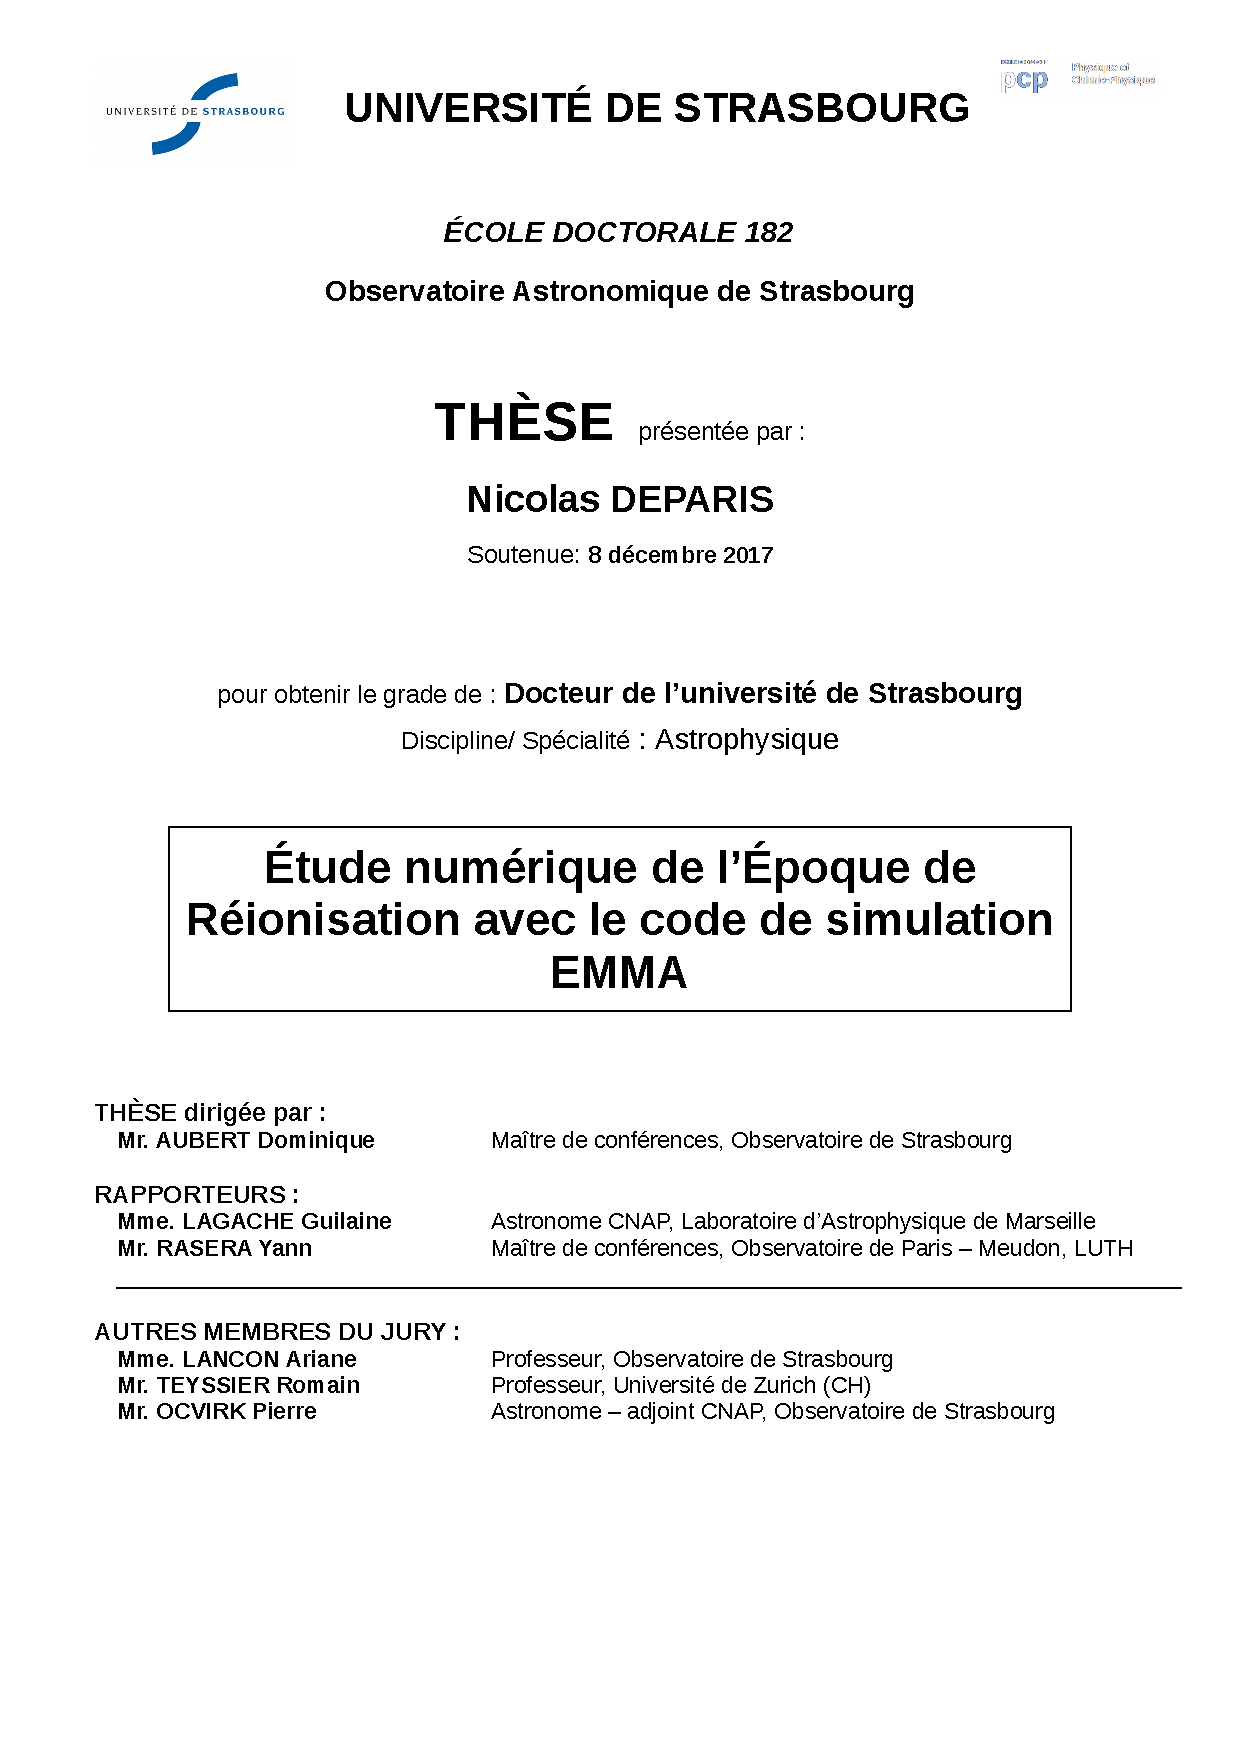
\includepdf{FrontBackmatter/couverture/1ere.pdf} 
%
%%%*******************************************************
% Little Dirty Titlepage
%*******************************************************
\thispagestyle{empty}
%\pdfbookmark[1]{Titel}{title}
%*******************************************************
\begin{center}
    \spacedlowsmallcaps{\myName} \\ \medskip                        

    \begingroup
        \color{Maroon}\spacedallcaps{\myTitle}
    \endgroup
\end{center}        

%%*******************************************************
% Titlepage
%*******************************************************
\begin{titlepage}
    % if you want the titlepage to be centered, uncomment and fine-tune the line below (KOMA classes environment)
    \begin{addmargin}[-1cm]{-3cm}
    \begin{center}
        \large  

        \hfill

        \vfill

        \begingroup
            \color{Maroon}\spacedallcaps{\myTitle} \\ \bigskip
        \endgroup

        \spacedlowsmallcaps{\myName}

        \vfill

        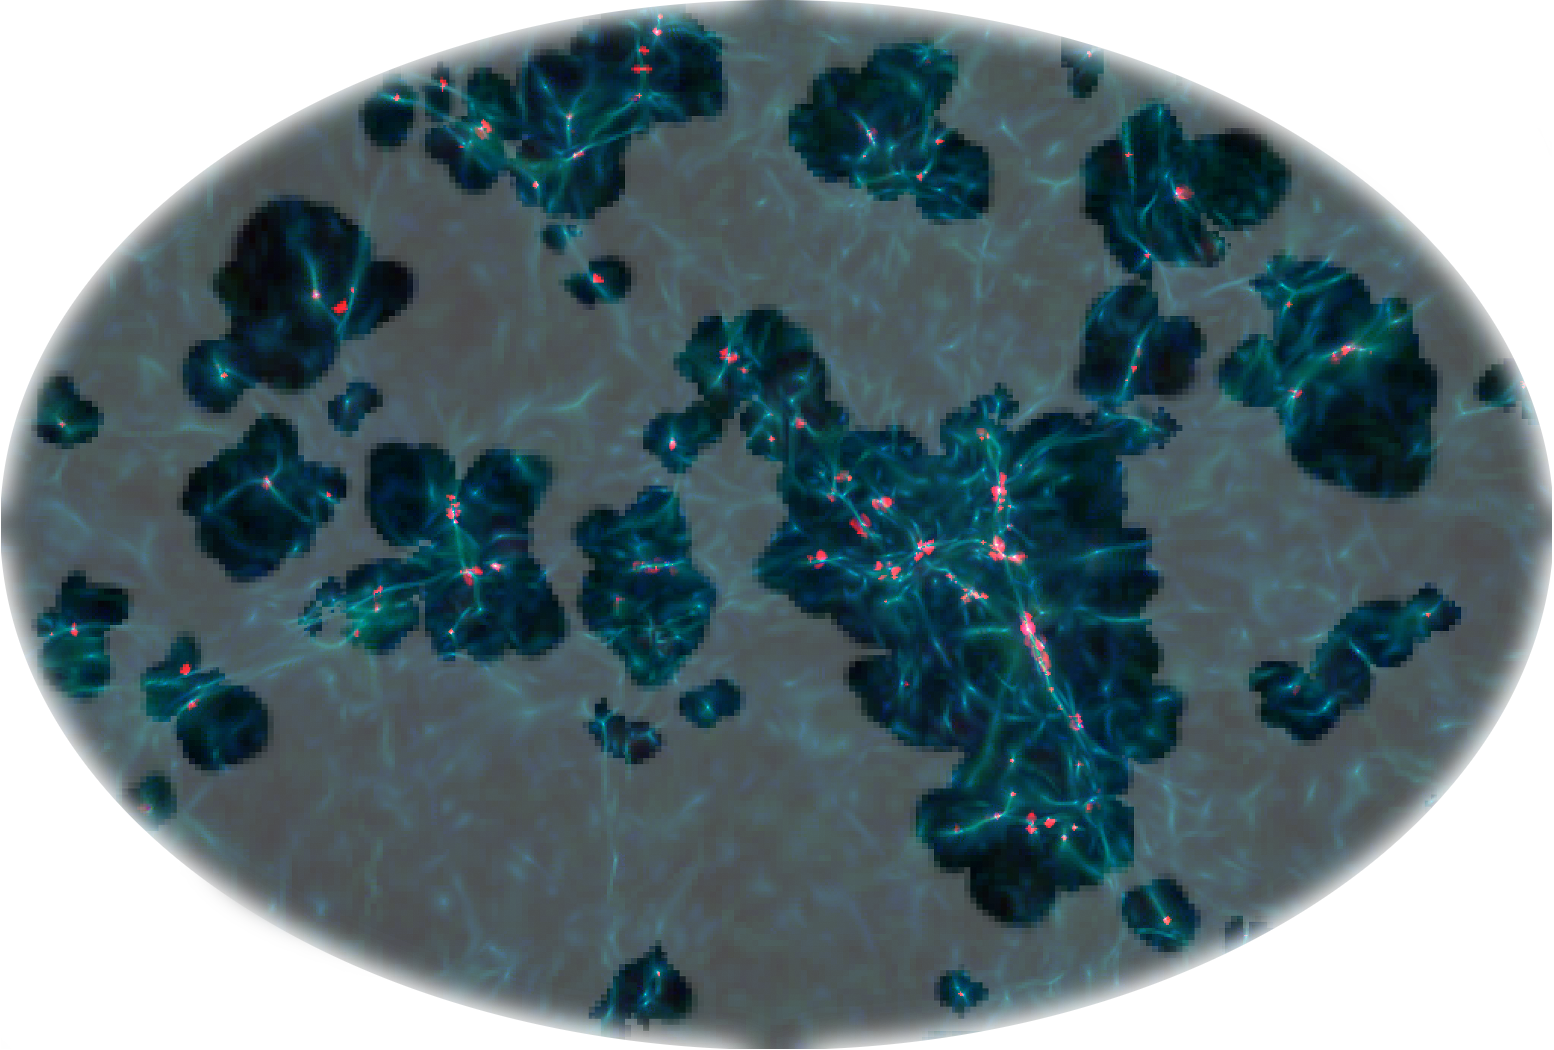
\includegraphics[width=12cm]{img/index.png} \\ \medskip

        \mySubtitle \\ \medskip   
        %\myDegree \\
        %\myDepartment \\                            
        %\myFaculty \\
        %\myUni \\ \bigskip

        \myTime\ -- \myVersion

        \vfill                      

    \end{center}  
  \end{addmargin}       
\end{titlepage}   
%\thispagestyle{empty}

\hfill

\vfill

\noindent\myName: \textit{\myTitle,} %\mySubtitle, %\myDegree, 
%\textcopyright\ 
\myTime

%\bigskip
%
%\noindent\spacedlowsmallcaps{Supervisors}: \\
%\myProf \\
%\myOtherProf \\ 
%\mySupervisor
%
%\medskip
%
%\noindent\spacedlowsmallcaps{Location}: \\
%\myLocation
%
%\medskip
%
%\noindent\spacedlowsmallcaps{Time Frame}: \\
%\myTime

%\cleardoublepage%*******************************************************
% Dedication
%*******************************************************
\thispagestyle{empty}
%\phantomsection 
\refstepcounter{dummy}
\pdfbookmark[1]{Dedication}{Dedication}

\vspace*{3cm}

\begin{center}
On fait la science avec des faits, comme on fait une maison avec des pierres; mais une accumulation de faits n'est pas plus une science qu'un tas de pierres n'est une maison. \\ \medskip
--- Henri Poincaré 
\end{center}

\vspace*{6cm}

\begin{flushright}
A Béatrice, Yann et Mariette.
\end{flushright}

%%\cleardoublepage\include{FrontBackmatter/Foreword}
%\cleardoublepage%*******************************************************
% Abstract
%*******************************************************
%\renewcommand{\abstractname}{Abstract}
\pdfbookmark[1]{Résumé}{Résumé}
\begingroup
\let\clearpage\relax
\let\cleardoublepage\relax
\let\cleardoublepage\relax

\chapter*{Résumé}
L’époque de réionisation (EoR) est une phase de grands changements qu’a subi l’Univers dans son premier milliard d’années. 
Suite à l’apparition des premières sources et à l’émission de photons énergétiques par ces dernières, l’hydrogène a été réionisé. 
Cette transition à eu un impact sur la formation des galaxies et leur contenance stellaire.

J’ai activement participé au développement d’EMMA, un code de simulation numérique aillant pour objectif d’étudier les processus a l’œuvre durant l’EoR. 
J’y ai développé et implémenté un modèle de formation et d’évolution stellaire et ces travaux ont contribué à la réalisation de "CoDa I AMR" une simulation dédiée à l’étude de l’EoR parmi les plus grandes réalisées à l’heure actuelle. 
J’ai également contribué au développement d’outils dédiés à l’exploration de simulations de ce type.

J’ai étudié la façon dont le rayonnement s’échappe des galaxies en fonction des paramètres du modèle stellaire, et montré qu'aux résolutions d’intérêt les supernovae peuvent augmenter la fraction de photons libérés.

J’ai également étudié la propagation des fronts d’ionisation et montré qu’il était possible de réduire la vitesse de la lumière par 3 (et ainsi diminuer le temps de calcul du transfert du rayonnement par 3), tout en conservant des résultats corrects.
CoDa I AMR a permis d'étudier le lien entre l'histoire de réionisation des halos et leurs masses actuelles.
Cette étude tend à confirmer l'hypothèse d'une réionisation précoce et interne du Groupe Local.


\vspace{0.5cm}

Mots clefs : Cosmologie, age sombres, réionisation, premières étoiles, méthodes numériques.
\vfill

\newpage

\begin{otherlanguage}{english}
\pdfbookmark[1]{Abstract}{Abstract}
\chapter*{Abstract}
The epoch of reionization (EoR) is a phase of big changes in the first billion years of the Universe history. After the apparition of the first stars and the emission of energetic radiation by thoses ones, the hydrogen was reionized. This transition has an impact on the galaxies formations.

I was part of the development team of EMMA, a numerical simulation code who aimed to study the  processes happening during the EoR. I developed and implement a stellar formation and evolution model. These works contributed to the realisation of "CoDa I AMR" one of the biggest simulation dedicated to the study of the EoR yet. I contribute to the development of a tool dedicated to the exploration of this kind of simulations.

I study how the radiation escaped the galaxies as a function of the parameters of the stellar model, and showed that supernovae could increase the ratio of escaping photon.

I also studied the ionization fronts propagation and showed that the speed of light could be reduced by a factor 3 (and then divide the computational cost of the radiative transfer by 3), while keeping corrects results.
CoDa I AMR was used to study the link between reionization histories and presents halos masses.
This study tends to confirm the hypothesis of an early and internal reionization of the Local Group.

\vspace{0.5cm}

Keywords : Cosmology, dark ages, reionization, first stars, numerical methods
\end{otherlanguage}

\endgroup			

\vfill





%%\cleardoublepage%*******************************************************
% Publications
%*******************************************************
\pdfbookmark[1]{Publications}{publications}
\chapter*{Publications}\graffito{This is just an early --~and currently ugly~-- test!}
This might come in handy for PhD theses: some ideas and figures have appeared previously in the following publications:

%\noindent Put your publications from the thesis here. The packages \texttt{multibib} or \texttt{bibtopic} etc. can be used to handle multiple different bibliographies in your document.

\begin{refsection}[ownpubs]
    \small
    \nocite{*} % is local to to the enclosing refsection
    \printbibliography[heading=none]
\end{refsection}

\emph{Attention}: This requires a separate run of \texttt{bibtex} for your \texttt{refsection}, \eg, \texttt{ClassicThesis1-blx} for this file. You might also use \texttt{biber} as the backend for \texttt{biblatex}. See also \url{http://tex.stackexchange.com/questions/128196/problem-with-refsection}.
%\cleardoublepage%*******************************************************
% Acknowledgments
%*******************************************************
\pdfbookmark[1]{Acknowledgments}{acknowledgments}

%\begin{flushright}{\slshape    
%    We have seen that computer programming is an art, \\ 
%    because it applies accumulated knowledge to the world, \\ 
%    because it requires skill and ingenuity, and especially \\
%    because it produces objects of beauty.} \\ \medskip
%    --- \defcitealias{knuth:1974}{Donald E. Knuth}\citetalias{knuth:1974} \citep{knuth:1974}
%\end{flushright}



\bigskip

\begingroup
\let\clearpage\relax
\let\cleardoublepage\relax
\let\cleardoublepage\relax
\chapter*{Acknowledgments}
Put your acknowledgments here.

Many thanks to everybody who already sent me a postcard!

Regarding the typography and other help, many thanks go to Marco 
Kuhlmann, Philipp Lehman, Lothar Schlesier, Jim Young, Lorenzo 
Pantieri and Enrico Gregorio\footnote{Members of GuIT (Gruppo 
Italiano Utilizzatori di \TeX\ e \LaTeX )}, J\"org Sommer, 
Joachim K\"ostler, Daniel Gottschlag, Denis Aydin, Paride 
Legovini, Steffen Prochnow, Nicolas Repp, Hinrich Harms, 
 Roland Winkler, Jörg Weber, Henri Menke, Claus Lahiri, 
 Clemens Niederberger, Stefano Bragaglia, Jörn Hees, 
 and the whole \LaTeX-community for support, ideas and 
 some great software.

\bigskip

\noindent\emph{Regarding \mLyX}: The \mLyX\ port was intially done by 
\emph{Nicholas Mariette} in March 2009 and continued by 
\emph{Ivo Pletikosi\'c} in 2011. Thank you very much for your 
work and for the contributions to the original style.


\endgroup




%\pagestyle{scrheadings}
%\cleardoublepage%*******************************************************
% Table of Contents
%*******************************************************
%\phantomsection
\refstepcounter{dummy}
\pdfbookmark[1]{\contentsname}{tableofcontents}
\setcounter{tocdepth}{2} % <-- 2 includes up to subsections in the ToC
\setcounter{secnumdepth}{3} % <-- 3 numbers up to subsubsections
\manualmark
\markboth{\spacedlowsmallcaps{\contentsname}}{\spacedlowsmallcaps{\contentsname}}
\tableofcontents 
\automark[section]{chapter}
\renewcommand{\chaptermark}[1]{\markboth{\spacedlowsmallcaps{#1}}{\spacedlowsmallcaps{#1}}}
\renewcommand{\sectionmark}[1]{\markright{\thesection\enspace\spacedlowsmallcaps{#1}}}
%*******************************************************
% List of Figures and of the Tables
%*******************************************************
\clearpage

\begingroup 
    \let\clearpage\relax
    \let\cleardoublepage\relax
    \let\cleardoublepage\relax
    %*******************************************************
    % List of Figures
    %*******************************************************    
    %\phantomsection 
    \refstepcounter{dummy}
    %\addcontentsline{toc}{chapter}{\listfigurename}
    \pdfbookmark[1]{\listfigurename}{lof}
    \listoffigures

    \vspace{8ex}

    %*******************************************************
    % List of Tables
    %*******************************************************
    %\phantomsection 
    \refstepcounter{dummy}
    %\addcontentsline{toc}{chapter}{\listtablename}
    \pdfbookmark[1]{\listtablename}{lot}
    \listoftables
        
    \vspace{8ex}
%   \newpage
    
    %*******************************************************
    % List of Listings
    %*******************************************************      
      %\phantomsection 
    \refstepcounter{dummy}
    %\addcontentsline{toc}{chapter}{\lstlistlistingname}
    \pdfbookmark[1]{\lstlistlistingname}{lol}
    \lstlistoflistings 

    \vspace{8ex}
       
    %*******************************************************
    % Acronyms
    %*******************************************************    
    \phantomsection 
    \refstepcounter{dummy}
    \pdfbookmark[1]{Acronymes}{Acronymes}
    \markboth{\spacedlowsmallcaps{Acronymes}}{\spacedlowsmallcaps{Acronymes}}
    \chapter*{Acronymes}
    \begin{acronym}[UMLX]
    \acro{AMR}{Adaptive Mesh Refinement}
	\acro{EoR}{Epoch of Reionization}
	\acro{DM}{Dark Matter}
	\acro{CIC}{Cloud In Cell} 
	\acro{SFR}{Star Formation Rate} 
	\acro{SFH}{Star Formation History} 
	\acro{IGM}{InterGalactic Medium} 
	\acro{UV}{UltraViolet} 
	\acro{IMF}{Initial Mass Function} 
	\acro{CRTA}{Coarse Radiative Transport Approximation} 
	\acro{DMP}{Dark Matter Particles} 
	\acro{IC}{Initial Condition} 
	\acro{OTSA}{On The Spot Approximation} 
    \acro{API}{Application Programming Interface}
    \acro{SPH}{Smooth Particle Hydrodynamic}
    \acro{GPU}{Graphical Processing Unit}
    \acro{CPU}{Central Processing Unit}
    \acro{RSLA}{Reduced Speed of Light Approximation}
    \acro{FOF}{Friend Of Friend}
    \acro{FOV}{Field Of View}
    \acro{FPS}{Frame Per Second}
    \acro{CMB}{Cosmic Microwave Background}
    \acro{RGB}{Red Green Blue}
    \acro{HDD}{Hard Drive Disk}
    \acro{SSD}{Solid State Drive}
    \acro{MUSCL}{Monotonic Upstream-Centered Scheme for Conservation Laws}
    \acro{HMF}{Halo Mass Function}
    \acro{GMF}{Galaxy Mass Function}
    \end{acronym}
\endgroup

%%********************************************************************
%% Mainmatter
%%*******************************************************
%\cleardoublepage\pagenumbering{arabic}
%%\setcounter{page}{90}
%% use \cleardoublepage here to avoid problems with pdfbookmark
%\cleardoublepage

%%%%%%%%%%%%%%%%%%%%%%%%%%%%%%%%%%%%%%%%%%%%%%%%%%%%%%%%%%%%%%%
%%%%%%%%%%%%%%%%%%%%%%%%%%%%%%%%%%%%%%%%%%%%%%%%%%%%%%%%%%%%%%%

%
\chapter*{Avant-Propos}

\begin{flushright}{\slshape    
	Une civilisation sans la science \\
	c'est aussi absurde qu'un poisson sans bicyclette.} \\ \medskip 
	--- Pierre Desproges
\end{flushright}

\vspace{0.5cm}
%\begin{itemize}
%\item la révolution industrielle
%\item migration vers les villes (50\% de la population mondiale depuis pas longtemps)
%\item déconnexion de la terre a cause du béton
%\item déconnexion du ciel a cause des éclairages publique
%\item étudier l'astrophysique est essentiel pour que l'Homme reste humble et considère sa place dans l'univers pour ne pas courir a sa perte.
%\end{itemize}

La question de la place de l'Humanité dans l'Univers a toujours été centrale et au cœur des préoccupations de toutes les civilisations.
De nombreuses cosmologies ont vues le jours au fil des siècles et des peuples.

%Toutes ont en commun 

Il fut un temps ou l'Homme n'avait d'autre choix que de cultiver les champs le jour et vivre dans l'obscurité la nuit.
Il existait un lien fort entre ce qui se passait sur terre (Humanité vient de Humus après tout) et dans le ciel.
Il ne pouvait que constater le ciel étoilé et se poser la question de la provenance des lueurs qui remplissent la voûte céleste.

Absence de lumière a toujours créer une peur de l'inconnu, cette fameuse peur du noir.
Depuis le XIX ème siècle et la revolution industrielle, il est devenu possible de s'affranchir de la nuit.
Et nous ne nous en sommes pas privé.

Nous vivons dans un monde ou plus de la moitié de la population mondiale vie dans des villes ou l'obscurité n'a pas sa place.
L’éclairage publique agis comme un écran qui nous bloque la vue du ciel, et par la même occasion inhibe cette sensation de vertige que l'on peu ressentir en le regardant.

Cette migration urbaine à aussi pour conséquence de nous couper du lien a la terre
Les villes sont presque intégralement étanchéifiée par du béton.

L'étude de la cosmologie et sa vulgarisation est une nécessité si l'on veux retrouver une certaine humilité vis a vis de notre seul et unique lieu de vie.


\vspace{0.5cm}


\begin{flushright}{\slshape    
	You devellop an instant global consciousess, \\
	a people orientation,\\
	an intense dissatisfaction with the state of the world,\\
	and a compulsion to do something about it.\\
	From out there on the moon, internationnal politic look so petty. \\
	You want to grab a politician by the scuff of the neck\\
	and drag him a quarter of a million mile out and say: \\
	'Look at that you son of a bitch'\\ \medskip 
	--- Edgar Mitchell Appolo 14 astronaut }
\end{flushright}
%\chapter{Introduction}
%Besoin des simu car contraintes observationnelles sur IGM mais impact fort sur les galaxies, pas le même timing, physique complexe il faut simulaer
%
%D'une manière générale, la méthode scientifique repose sur 3 piliers: 
%\begin{enumerate}
%\item L'observation
%\item La théorie
%\item L'expérience
%\end{enumerate}
%L'astrophysique moderne n’échappe pas à cette règle.
%
%\paragraph{L'observation} est le plus ancien des piliers, et constitue le point de départ de toute démarche scientifique.
%L'Homme a toujours regardé le ciel, et avant même de chercher à le comprendre, il a recueilli des informations à son sujet. %le regarder et l'analyser.
%Contrairement aux autres discipline scientifique, le point de vue que nous avons sur notre sujet d'analyse est unique, il nous est impossible d'observer l'Univers sous un autre angle.
%%Les techniques d'observations ont fait d’énormes progrès ces dernières années, mais observer ne suffit pas.
%
%%Il celui sur lequel repose le plus de poids puisque tout en découle.
%%De plus il est commun a toute les disciplines scientifique.
%%Il n'est pas de science possible sans observation.
%
%\paragraph{La théorie} est le deuxième piliers.
%%Lorsque l'on voit ces lumière sur la voûte céleste, nous sommes obligé de nous poser la question essentielle de leur provenance.
%%Cette question mène a l'élaboration de diverse formulation tentant d'expliquer comment (et pourquoi) le ciel s'illumine la nuit.  
%%Dans le cadre de l'étude de l'univers dans sont ensemble, cette théorie est nommée cosmologie et repose sur des concept mathématiques complexes
%L'objectif est ensuite de réussir à donner un sens aux informations récoltées et de prédire les prochaines observations.
%%Au fil des siècles, diverses théories ont été élaborées pour expliquer le comportement de l'Univers observable.
%En effet, la force d'une théorie est jugée à sa capacité à faire des prédictions.
%%A partir de la théorie, on réalise un modèle, un ensemble de règles  permettant de définir l'évolution d'un système connaissant son état actuel.
%
%\paragraph{L'expérience} est le dernier pilier.
%D'une manière générale, l'expérience a pour but de mettre a l’épreuve la théorie, et représente un ensemble d'actions, réalisées en suivant un protocole, permettant d'obtenir des résultats reproductibles.
%A l'inverse d'autres domaines scientifique, en astrophysique notre portée d'interaction est réduite.
%Il ne nous est ni possible d'effectuer des expériences sur l'Univers, ni de changer notre point d'observation.
%Les simulations numériques permettent de palier à ces problèmes en créant virtuellement des portions d'espace respectant un certain modèle.
%Un modèle, étant un ensemble de règles, issues de la théorie et permettant de définir l'évolution d'un système en connaissant son état actuel.
%%Pilier le plus récent il est sensé palier au problème des deux autres : l'impossibilité de changer de point de vue ou de tester les théories élaborées.
%%Ici sous entendue la simulation numérique, il est beaucoup plus récente et dépend grandement de la technologie.
%%C'est celui vers lequel j'ai choisis de me diriger.
%
%%observation, modélisation et test de la théorie or en astro on ne peut pas tester directement donc on simule.
%
%\paragraph{}
%
%Cette thèse est articulée principalement autour du dernier pilier.
%Une grande partie de cette thèse a été consacrée à l'élaboration d'un modèle numérique dédié à l'étude de la réionisation.
%Puis, dans le but d'explorer ce modèle, un nombre important d'expériences (de simulations) ont été réalisées.
%Dans cette première partie, je vais introduire quelques grands concepts liés a l'étude numérique de la réionisation, puis je présenterai la structure du présent manuscrit en m'appuyant sur ces concepts.
%
%\subsection*{Le modèle standard}

Notre compréhension actuelle de l'Univers s'inscrit dans le cadre du modèle standard de la cosmologie.
Ce modèle repose sur un Univers non statique et en expansion, ayant une origine, le Big-Bang.
Très tôt dans son évolution, l'Univers était extrêmement chaud et dense, il n'y avait alors ni étoiles ni galaxies.
Après l'émmission du fond diffus cosmologique 380000 ans Big-Bang, l'Univers était froid et majoritairement composé de gaz neutre.
%Mais sous l'effet de l'expansion, le plasma primordial s'est refroidi, les premiers atomes se sont formés lors de ce que l'on nomme la recombinaison, qui a mené à l'émission du fond diffus cosmologique.
%L'Univers était alors extrêmement homogène que ce soit en densité ou en température, mais cette homogénéité n'était pas parfaite.
%S'en suit une période où les in-homogénéités primordiales se sont effondrées sur elles même du fait de la gravité.
%Puis, environ trois cents millions d'années après le Big-bang ces in-homogénéités sont devenues suffisamment denses pour former les première étoiles.
%Ces étoiles ont émis un rayonnement suffisamment énergétique pour séparer les électrons et les protons liés au moment de la recombinaison.
%L'univers c'est alors retrouvé une nouvelle fois dans un état majoritairement ionisé : c'est ce que l'on nomme la réionisation.
%\subsection*{La réionisation}
%La réionisation constitue le dernier grand changement que l'univers ai subit lorsqu'il était âgé de moins d'un milliard d'années.
L'effondrement gravitationnel du gaz qui a permit par endroits une élévation de densité et de température suffisante pour réamorcer des réactions de fusion thermonucléaire est à l'origine de la formation des premières générations d'étoiles,
%Il s'agit de la première génération d'étoiles.
%Le matériaux disponible pour leurs formations était alors abondant.
%On pense que ces étoiles étaient beaucoup plus massives, et donc beaucoup plus énergétique que les étoiles observées actuellement.
%Cette première génération 
qui ont émis un rayonnement ultraviolet ionisant qui a grandement impacté le milieu environnant : c'est cette étape que l'on nomme la réionisation.%, en le chauffant et en l'ionisant. % par effet thermique et en le déplaçant par effet de pression de radiation.
La réionisation n'est pas un processus instantané, et il est estimé aujourd'hui que les premières étoiles sont apparues alors que l'Univers était âgé d'environ 300 millions d'années. 
Il fallut alors 700 millions d'années supplémentaires pour que le rayonnement remplisse l'Univers, situant ainsi la fin de la période de réionisation à environ un milliard d'années après le Big-bang.

%
%De plus, à la fin de leur vie, ces étoiles massives ont explosé en supernovæ, effectuant alors un puissant chauffage ainsi qu'un fort brassage du gaz.
%En changeant la configuration du milieu, ces premières étoiles ont modelées les lieux d'apparition des générations suivantes et par effet de cascade a eu un impact sur la distribution de matière observée aujourd'hui.
%
%%La vitesse de la lumière étant finie, il fallut un certain temps pour que les premiers rayons ionisant puisse atteindre tous les recoins de l'Univers. 
%
%%C'est cette transition entre un univers neutre et froid vers un univers chaud et ionisé que l'on appel l'époque de réionisation.
%%L'apparition des première sources lumineuse a eu un impact sur la façon dont la matière c'est organisée pour former les galaxies.
%%Il est probable que l'univers que l'on observe aujourd'hui, ai conservé les traces de cette grande époque de transition.
%
%Une des difficulté à l'étude de la réionisation est l'époque à laquelle elle s'est produite. %on considère actuellement qu'elle a eu lieu dans le premier milliard d'année de l'univers.
%Pour observer l'Univers jeune, il faut regarder loin, et les meilleurs télescopes actuels ne sont pas encore assez performants pour atteindre des époques aussi lointaines.
%Il faudra attendre encore au moins une décennie avant la mise en place des prochaines générations de télescopes assez puissants pour observer les environnements de formation de ces premières sources lumineuses.
%
%\subsection*{Les simulations numériques}
%
%Les premières simulations cosmologiques ne considéraient l'évolution que de la matière noire. %la composante non collisionnelle de la matière, ie .
%Comme celle ci constitue la masse la plus abondante de l'Univers, ces simulations permettent de suivre l'évolution de la distribution de matière sur les grandes échelles. 
%Mais comme la matière noire est invisible, il manquait une composante importante : les baryons.
%Lorsque l'intérêt fut porté sur la formation des galaxies, le calcul de l'hydrodynamique du gaz fut alors introduit, puis avec lui les premiers modèles de formation stellaire apparurent.
%Mais la communauté a vite été confrontée a un important problème: le gaz refroidissait trop.
%Ce qui menait à une formation d'étoile trop abondante car rien n’empochait le gaz de s’effondrer sur lui même.
%Pour palier à ce problème, il fut proposé d'injecter de l'énergie dans les endroits les plus denses.
%Cette énergie, introduite par les supernovæ, permet de chauffer le gaz et ralenti son effondrement. 
%%Depuis très récemment, une troisième physique est devenue  dans les simulations l'influence de la radiation sur le milieu est également prise en compte.
%Aujourd'hui, l'intérêt est porté sur l'introduction d'une nouvelle physique, celle du rayonnement.
%Le rayonnement émit par les étoiles, va changer les propriétés physico-chimique et thermique du gaz qui les environnent et ainsi modeler les lieux d'apparitions des générations futures d'étoiles.
%
%Même si les possibilités d'observations sont restreintes, nous pouvons utiliser les simulations numériques pour tenter de comprendre les phénomènes en cours à cette époque.
%En effet, les phénomènes en action pendant la réionisation sont nombreux et les modèles analytique trouvent leurs limites.
%Avec l'avancée exponentielle des capacités de calculs, les ordinateurs se transforme petits a petit en véritable laboratoire pour les astrophysiciens.


\paragraph{}
Voici un aperçu de ces questions que nous allons aborder dans cette thèse: 

\begin{itemize}
\item Quelles sont les physiques nécessaires à la bonne modélisation de l'époque de la réionisation ?
\item À quelles échelles ces phénomènes interviennent t il ?
\item Comme la formation stellaire des premières générations d'étoiles à impactée l'apparition des générations suivantes ? %le déroulement de la réionisation ?
\item Quel impact la réionisation a elle eu sur la formation des galaxies ?
\item Comment s'est propagée l'ionisation dans l'Univers ?
\item Y a t-il des marques de la réionisation dans l'Univers local ?
\item L'Univers a t-il été réionisé par quelques grosses sources très lumineuses ou par de nombreuses sources moins énergétiques ?
\end{itemize}

Pour étudier des phénomènes aussi fortement couplés que ceux considérés dans le cas de l'époque de réionisation, il est nécessaire d'avoir recours à des simulations numériques. 
%Le but de ces simulations est de reproduire les observations sur la distribution de matière dans l'Univers.
A l'heure actuelle, il commence à être possible de simuler de manière auto cohérente, l'effondrement de structures cosmologiques, contenant du gaz, formant des étoiles, qui émettent du rayonnement.
%Ces simulations ont pour objectif d'aider à comprendre quelques unes des grandes questions en suspend dans l'étude de la réionisation.
Mais l'utilisation de simulation introduit également quelques question : 

\begin{itemize}
\item Comment simuler la réionisation efficacement ?
\item Comment modéliser au mieux les différents physiques à l’œuvre ?
\item De quelle résolution à t-on besoin ?
\item Comment tirer profit au maximum du matériel disponible ?
\item Quels sont les compromis nécessaire ?
\end{itemize}

%\begin{itemize}
%\item Quand sont apparues les premières sources lumineuses?
%Nous verrons que les observations imposent certaines contraintes sur la fin de la réionisation mais nous n'avons actuellement que très peu de contraintes sur la durée du processus.
%
%\item L'Univers a t-il été réionisé par quelques grosses sources très lumineuses ou par de nombreuses sources moins énergétiques ?
%La question reste ouverte de savoir si se sont les quasars, sources relativement rares mais pouvant être extrêmement énergétiques, ou les galaxies plus modestes mais beaucoup plus nombreuses?
%Dans le cas où se serait les galaxies, serait-ce les plus légères, extrêmement nombreuses ou les plus massives?
%
%\item Comment ces premières générations d'étoiles ont influencées l'apparition des suivante, et ont elles laissées des traces encore visibles dans l'environnement proche?
%
%\end{itemize} 

%En répondant à certaines de ces questions, les simulations numériques permettent de mieux cibler les futures missions d'observations, et augmentent les chances de réussites.

%En étudiant au préalable ce que l'on cherche à observer, on a plus de chance d'observer au bon endroit et de la bonne facon.

%Au stade actuel de notre compréhension de l'univers, les simulations numériques ont a la fois de très belles réussites mais souffres également de 

%\subsection*{Le groupe local}
%Le groupe local est un ensemble de quelques dizaines de galaxies, dont les principales représentantes sont la Voie Lactée et notre voisine Andromède.
%Il s'agit de notre environnement galactique proche.
%Ce qui le rend facilement observable.
%L'observation de cet environnement nous fournis des informations essentielles sur la cosmologie de l'Univers.
%
%Plus la precision des observations augmente, plus il est nécessaire d'avoir des simulations résolues disposant de toutes la physique nécessaire pur expliquer globalement les échelles considérées.
%Les premières simulations de matière noires ont permit d'expliquer les observations réalisées sur la distribution de la matière aux grandes échelles.
%Lorsque les capacité de calcul se sont révélées suffisantes pour explorer des résolutions plus fines, il est vite apparu un certain décalage entre simulation et observation. 
%L'introduction de l'hydrodynamique a permis d'augmenter l'accord entre les deux, jusqu'à un second palier de résolution.
%Aujourd'hui, l'introduction de la physique du rayonnement va certainement permette de diminuer encore les échelles auxquelles les simulations sont sont en accord avec les observations.
%L'ordre de grandeur de ces échelles est celui de la taille du groupe local.
%
%De plus, les échelles que l'on considère dans les simulations cosmologiques a rayonnement couplé se rapproche de plus en plus des échelles considérés dans les simulations d'évolution de galaxies.
%L'objectif est ici de faire le lien entre la physique de l'univers dans son ensemble (la cosmologie) et de la physique régissant l'évolution de notre galaxie ou de sa voisine (la physique galactique).


\section{Mes travaux}

Dans l'objectif de répondre à certaine de ces questions, il est nécessaire de développer des outils.
EMMA, un code de simulations cosmologiques dédié à l'étude de la réionisation, à été mon principal outil durant cette thèse.
J'y ai apporté différentes contributions, allant de l'ajout de nouvelles fonctionnalités jusqu'à la simple résolution de conflits, en passant par l'optimisation de certaine parties.

Une de mes principales contributions a été l'implémentation d'un modèle de formation et d'évolution stellaire et une étape importante de cette thèse a été sa calibration..
Ce modèle dispose de plusieurs paramètres libres, et leurs valeurs étant directement fonction de la résolution, il a naturellement été choisi d'utiliser la résolution des plus grosse simulations à l'heure actuelle.
Cette calibration a été une étape préliminaire à la réalisation de la simulation CODA I-AMR une des plus grosse simulation de la réionisation à l'heure actuelle.
% une simulation représentant un volume de $(100 cMpc)^3$ échantillonné par $2048^3$ éléments de résolutions et une résolution adaptative allant jusqu'à 500pc.
%Les ressources de calculs étant limitées, il est nécessaire de faire certaines concessions, le choix doit être fait entre volume physique et résolution.
Les ressources de calculs étant limitées, il n'est pas possible de réaliser plusieurs de ces simulations.
Or la calibration nécessite un grand nombre de tests, j'ai pour cella exécuté des simulations de taille réduite à $(12 cMpc)^3$ avec une résolution comparable à celle de la simulation CoDa I AMR. 
L'objectif est d'explorer une partie de l'espace de paramètres du modèle, et de comprendre, sur des échantillons, quel est l'influence des paramètres libres sur les résultats obtenus, et leur interprétation dans des simulations plus grandes.

%Pour analyser les nombreuse simulations obtenues dans de bonnes conditions, j'ai développé une librairie pour d'analyse et la gestion des données.
%Cette librairie rassemble une grandes part des outils d’analyse que j'ai développé et est en accès libre, pour faciliter l'accès d'EMMA à ses nouveaux utilisateurs.
%visu

Dans l'objectif de diminuer les concessions à réaliser sur la taille et la résolution des simulations, il existe différentes pistes : soit augmenter l'accès aux ressources de calculs, soit optimiser les codes de simulations.
Un des mes objectif a été de mieux cerner l'ensemble des techniques utilisées dans un tel code pour être en mesure de cibler au mieux les points à améliorer.

Il existe entre autre une technique consistant à diminuer numériquement la vitesse de la lumière pour réduire artificiellement, la charge de calcul.
Je me suis posé la question du domaine de validité de cette approximation, et du gain maximum que l'on peut espérer grâce à cette technique tout en restant dans un domaine d'approximation raisonnable.

%\textit{Quels sont les facteurs qui limitent la performance globale de EMMA et comment les améliorer?}
%
%Une autre piste n'est pas algorithmique mais matérielle.
%L'utilisation de processeurs graphique permet dans certain cas des accélération considérable (jusqu’à deux ordre de grandeurs).
%Cependant l'utilisation de ce matériel impose certaines précaution et si une grande partie d'EMMA l'utilise déjà, le potentiel d'accélération reste grand.


\section{Organisation du manuscrit}
%\begin{itemize}
%\item Introduction au   cosmologique $\Lambda$ CDM et a la période de réionisation.
%\item Présentation du model numérique (Papier emma)
%\item Présentation du model d'étoiles (papier SN)
%\item Présentation de l'outils des cartes de reionization (papier c)
%\item 
%\end{itemize}

Ce manuscrit est articulé autour de différents travaux auxquels j'ai contribué durant ma thèse.
Après le présent chapitre introductif, la première partie sera consacrée à la mise en place du contexte.
Une fois les grandes lignes du modèle physique introduites, et le contexte de la réionisation posé, j'aborderai plus spécifiquement mes travaux.
Je m'appuierai sur chacune des publications auxquelles j'ai contribué, et articulerai un chapitre autour de chacune d'elles. 

\paragraph{Contexte :}
Le chapitre \ref{ch:introduction_physique} constitue une introduction aux concepts utiles en cosmologie.
Ces concepts seront nécessaires pour aborder le chapitre \ref{sec:introreio} qui explore plus spécifiquement la période de réionisation.

\paragraph{Méthodes numériques :}
Une partie sera consacrée à EMMA l'outil central de cette thèse.
%, un code capable de simuler l'évolution de la matière noire, du gaz et de la radiation à des échelles cosmologiques de manière entièrement couplé, et ayant pour principal objectif l'étude de la période de réionisation.
Dans le chapitre \ref{ch:introduction}, je commencerai par présenter les grandes lignes de \emma, et introduirai sa maille adaptative qui contraindra plusieurs choix par la suite.
Le chapitre \ref{sec:solvers} sera consacré au développement des différents moteurs physiques et de leurs concepts numériques associés.
Puis dans le chapitre \ref{sec:materiel}, l'accent sera mis sur les techniques de parallélisation utilisées dans EMMA qui a la particularité d'être massivement parallèle et d'être accéléré par processeurs graphiques.
Cette approche permettra au lecteur de mieux appréhender les résultats obtenus à partir des simulations générées ensuite avec ce code.

\paragraph{Modèle stellaire :}
Comme l'étude du rayonnement émis dans l'Univers passe immanquablement par l'étude de la formation stellaire, je consacrerai le chapitre \ref{sec:etoiles} à détailler le modèle de formation et d'évolution stellaire de EMMA, ainsi que ses contraintes, ses limites, et les différents tests qui ont été exécutés pour sa calibration.
Je présenterai ensuite dans le chapitre \ref{sec:galaxies} une étude que j'ai menée à l'aide de ce modèle, visant à mieux comprendre la physique à l'œuvre dans les grandes simulations de la réionisation.
L'objectif est de comprendre quelles sont les galaxies qui contribuent à la réionisation dans nos modèles et quel est l'impact du feedback stellaire sur cette contribution.

\paragraph{Cartes de réionisation :}
Le chapitre \ref{sec:intre:zreio} sera consacré à une étude sur l'influence de l'approximation de la vitesse de la lumière réduite sur la propagation des fronts d'ionisation.
Nous verrons que dans les simulations de la réionisation, la vitesse de la lumière peut être changée de manière à économiser du temps de calcul.
J'ai cherché a quantifier dans quelle mesure celle ci peux être réduite avant que cela ai un impact sur les résultats des simulations.
Pour cela j'ai développé un méthode pour calculer la vitesse des fronts d'ionisation, en utilisant les cartes de réionisation, outils qui sera également introduit dans cette partie.

Le chapitre \ref{sec:CODAEMMA} sera dédié à la présentation de la simulation "CoDa II AMR". %, une des plus grosse simulation de la réionisation à l'heure actuelle.
J'y présenterai les premiers résultats obtenus à propos du liens entre la masse des halos contenus dans la simulation aujourd'hui et leurs histoires au moment de la réionisation.
Cette étude sera menée à l'aide des cartes de réionisation.

\paragraph{Visualisation : }
Nous verrons ensuite un court chapitre  \ref{sec:visu}, consacré à la présentation de travaux liés à la visualisation des simulations cosmologiques.
J'y aborderai différentes méthodes de visualisations ainsi que quelques détails technique liés à leurs implémentations.

%Ce modèle constitue une de mes principale contributions à \emma.
%J'ai implémenté dans \emma, un modèle de transformation du gaz en particule stellaire.
%Ce modèle se base sur un critère de densité pour 
%Lorsque, sous l'effet de la gravitation, une cellule devient suffisamment dense, celle ci devient autorisée à former des étoiles.
%Toute les cellules autorisées vont alors transformer une certaine quantité du gaz en particule stellaire, en fonction de l'état local de la cellule, et suivant une loi empirique issue de l'observation : la loi de Schmidt-Kennicutt.
%Les particules nouvellement créées vont alors émettre du rayonnement ionisant pendant un certain temps.
%A la fin de leurs vie, ces particules stellaires vont exploser en supernovæ, injectant ainsi une quantité non négligeable d'énergie dans le milieu environnant.
%Cette énergie supplémentaire perturbe le milieu et régule la formation stellaire.
%J'ai implémenté différents modèles d'injection d'énergie dans le solveur hydrodynamique d'\emma{ } et comparé ces modèles entre eux. 

%Comme ces modèles nécessite l'introduction de plusieurs paramètres libres, une partie importante du temps a été consacrée à l'exploration et à la calibration de ces paramètres.


%Ce modèle considère deux types d'énergie. 
%La première, thermique, va dissiper une certaine partie de l'énergie disponible dans le chauffage du gaz.
%La seconde, cinétique, va mettre en mouvement le gaz environnant avec le reste de l'énergie.
%Une certaine proportion de la masse de la particule stellaire est retournée dans le milieu. 
%L'énergie totale et la masse des éjectas étant contrainte par un autre modèle, Starburst99.



%J'ai contribué à différents aspects du code mais une de mes 
%Au moment de mon arrivé en thèse,
%D'une manière plus générale j'ai contribué à divers aspect du code, comme la gestion des paramètres utilisateur, l'écriture des données de sorties ou encore la documentation.
%Dans la première partie de ma thèse, ma tache principale a été d'implémenter un scénario de formation stellaire, ainsi qu'un modèle de feedback de supernovae.
%Je développe également une librairie d'analyse des fichiers générés par \emma.


%J'ai également contribué au développement d'un code de visualisation et d'exploration de simulations astrophysique.


%
%\subsection*{Mod\`ele de formation stellaire}

%
%\subsection*{Mod\`ele de supernovae}
%
%Historiquement, les modèles de formation stellaire se sont rapidement confronté à un problème majeur : ils n'arrivaient pas à reproduire les observations en terme de quantité d'étoiles crées.
%Une réponse à ce problème fut l'introduction des supernovaes. 

%
%De la même manière que précédemment, l'implémentation de ce modèle a introduit plusieurs paramètres libres qu'ils a fallut calibrer.
%
%A partir de ce modèle numérique j'ai ensuite réalisé plusieurs études:
%
%\begin{itemize}
%\item en faisant varier le modèle de feedback stellaire j'ai tenté de quantifier son influence sur le déroulement du processus de réionisation.
%\item J'ai étudié la vitesse de propagation des fronts d'ionisations et montré que le reionisation s'éffectue en 2 phases. 
%\item Le develloppement de ce modèle a conduit a la réalisation de l'une des plus grosses simulations de la réionisation a l'heure actuelle la simulation CODA-EMMA.
%J'introduirais cette simulation ainsi que les premiers résultats obtenus.
%\item Enfin, je présenterai mes travaux concernant la visualisation de données de simulations.
%\end{itemize}
%


%%%%%%%%%%%%%%%%%%%%%%%%%%%%%%%%%%%%%%%%%%%%%%%%%%%%%%%%%%%%%%%
%%%%%%%%%%%%%%%%%%%%%%%%%%%%%%%%%%%%%%%%%%%%%%%%%%%%%%%%%%%%%%%

%\part{Contexte}
%
\chapter{Le modele standard de la cosmologie moderne}
 \label{ch:introduction_physique}

Cette thèse s'inscrit dans le cadre du modèle standard de la cosmologie.
Ce modèle, aussi appelé modèle du Big-Bang, ou $\Lambda$CDM, considère un univers en expansion et composé essentiellement d'énergie noire ($\Lambda$) et de matière noire froide (Cold Dark Matter). 
Ce chapitre a pour objectif de présenter les grandes lignes de ce modèle.

\section{Émergence de l'idée d'un Univers non statique}

%découverte des galaxies\\
%découverte de l'expansion de l'univers

%\subsection{Cadre théorique}

L'idée d'un univers non statique a pris forme dans le début du XXème siècle suite à deux événements majeurs.
D'un coté l'élaboration de la théorie de la relativité générale d'Einstein en 1915 à permis la mise en place d'un cadre théorique propice.
%La notion d'un univers non statique a ete introduite par Einstein en 1917 en rapport avec ses travaux sur le relativité générale. 
D'un autre coté, plus d'une décennie plus tard les observations de Hubble ont confirmées l'expansion de l'Univers.

\subsection{Les observations de Hubble}

Entre 1923 et 1929 Hubble observe deux phénomènes qui vont mener à une redéfinition de notre notion de cosmologie.
Il bénéficie à l'époque de l'accès au plus puissant télescope du monde (le télescope Hooker du mont Wilson).
Cet instrument lui a permis, dans une publication de 1926, d'observer que des nébuleuses situées hors de notre galaxie présente des caractéristiques identiques à des système d'étoile \citep{1926ApJ....63..236H}.
Il en déduit qu'il existe d'autres galaxies que notre Voie Lactée (voir figure \ref{fig:hubbl_deep_field}).

%Avec les moyens observationnels dont nous disposons aujourd'hui l’existence d'un grand nombre de galaxies en dehors de notre voie lactée est bien établie.
%Le "Hubble Ultra Deep Field"  (voir figure \ref{fig:hubbl_deep_field}) une image prise en 2004 et publiée en 2006 \citep{1538-3881-132-5-1729} montre un grand nombre de galaxies dans une portion réduite du ciel.
%On estime aujourd'hui le nombre de galaxies à $\approx 2 \cdot 10^{11}$ dans l'Univers observable.

\begin{figure}
        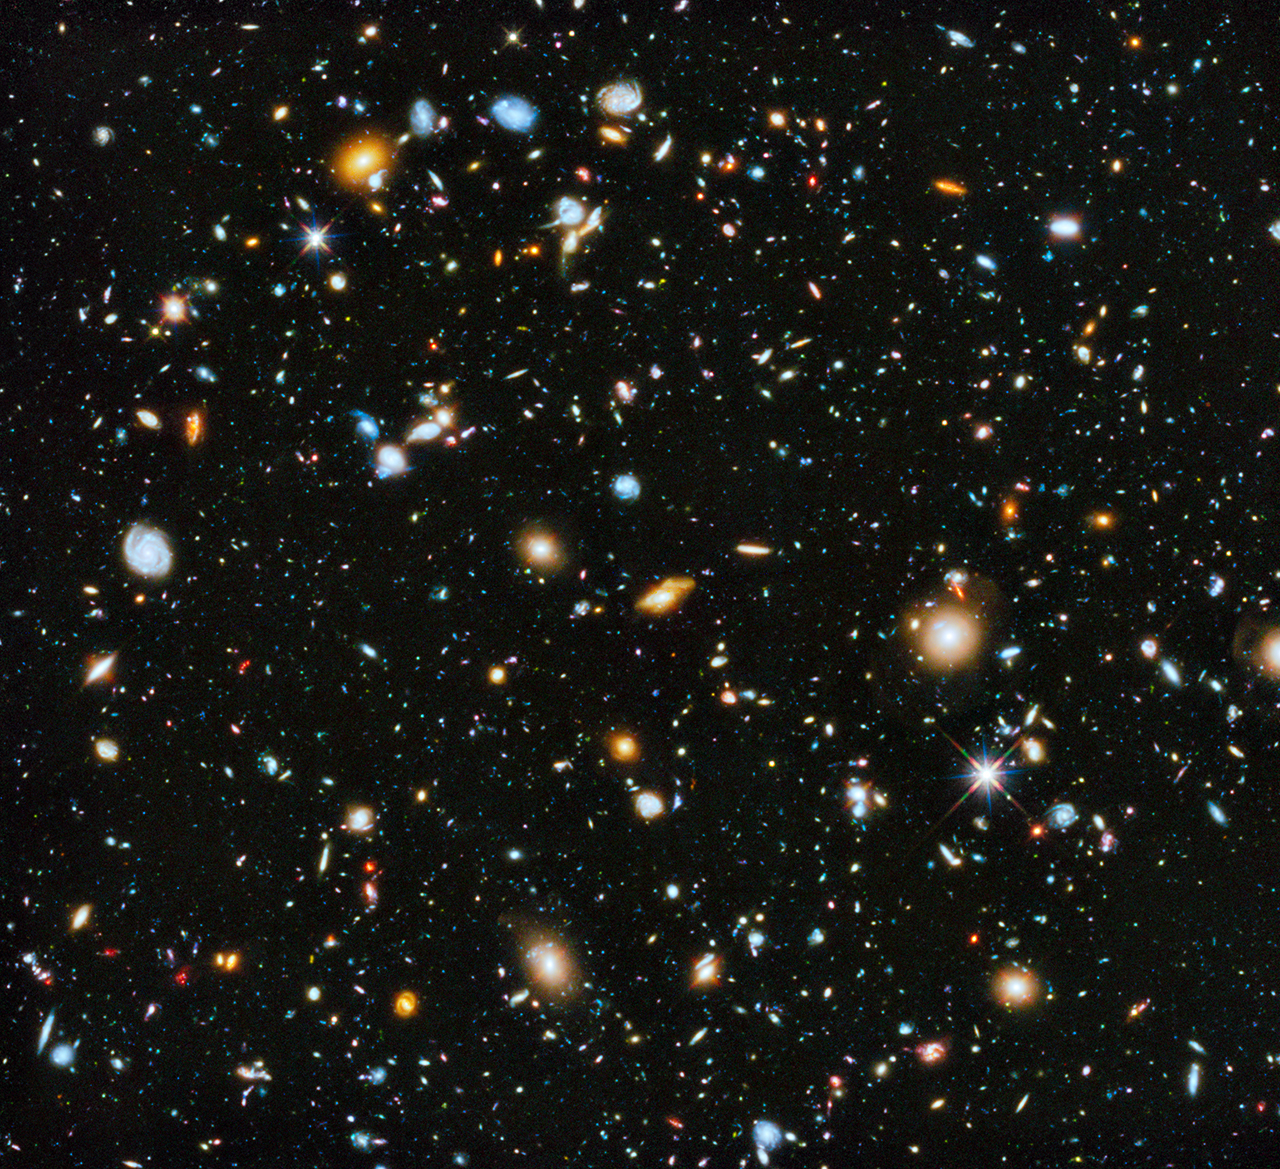
\includegraphics[width=.9\linewidth]{img/01/hudf.jpeg} 
        \caption[Hubble Ultra Deep Field]{Hubble Ultra Deep Field \citep{1538-3881-132-5-1729}.
        %2014.
        %Image NASA.
		En 1926 E. Hubble observe pour la première fois qu'il existe d'autre galaxies.
		Leur nombre est estimé aujourd'hui à $\approx 2 \cdot 10^{11}$ dans l'Univers observable.
 		\label{fig:hubbl_deep_field}}
\end{figure}

\subsection{La loi de Hubble}
Hubble observe également une relation entre la distance de ces nouvelles galaxies et leurs spectres lumineux \citep{1929CoMtW...3...23H}.
Plus une galaxie est éloignée de l'observateur, plus son spectre est décalé vers le rouge.
%Ce redshift noté $z$ est une notion qui sera beaucoup utilisée par la suite car nous verrons dans la prochaine section qu'il existe un lien direct entre âge de l'univers et redshift.
%Il interpréta ce décalage comme un effet Doppler et montra que ces galaxies s'éloignent de l'observateur avec une vitesse radiale directement proportionnelle à leur distance.
%Cette corrélation entre la distance et le décalage vers le rouge observé est aujourd'hui bien établie (voir figure \ref{fig:hubble_law}).
%Une série d'observations récentes est présenté sur la .
%
%\begin{figure}
%        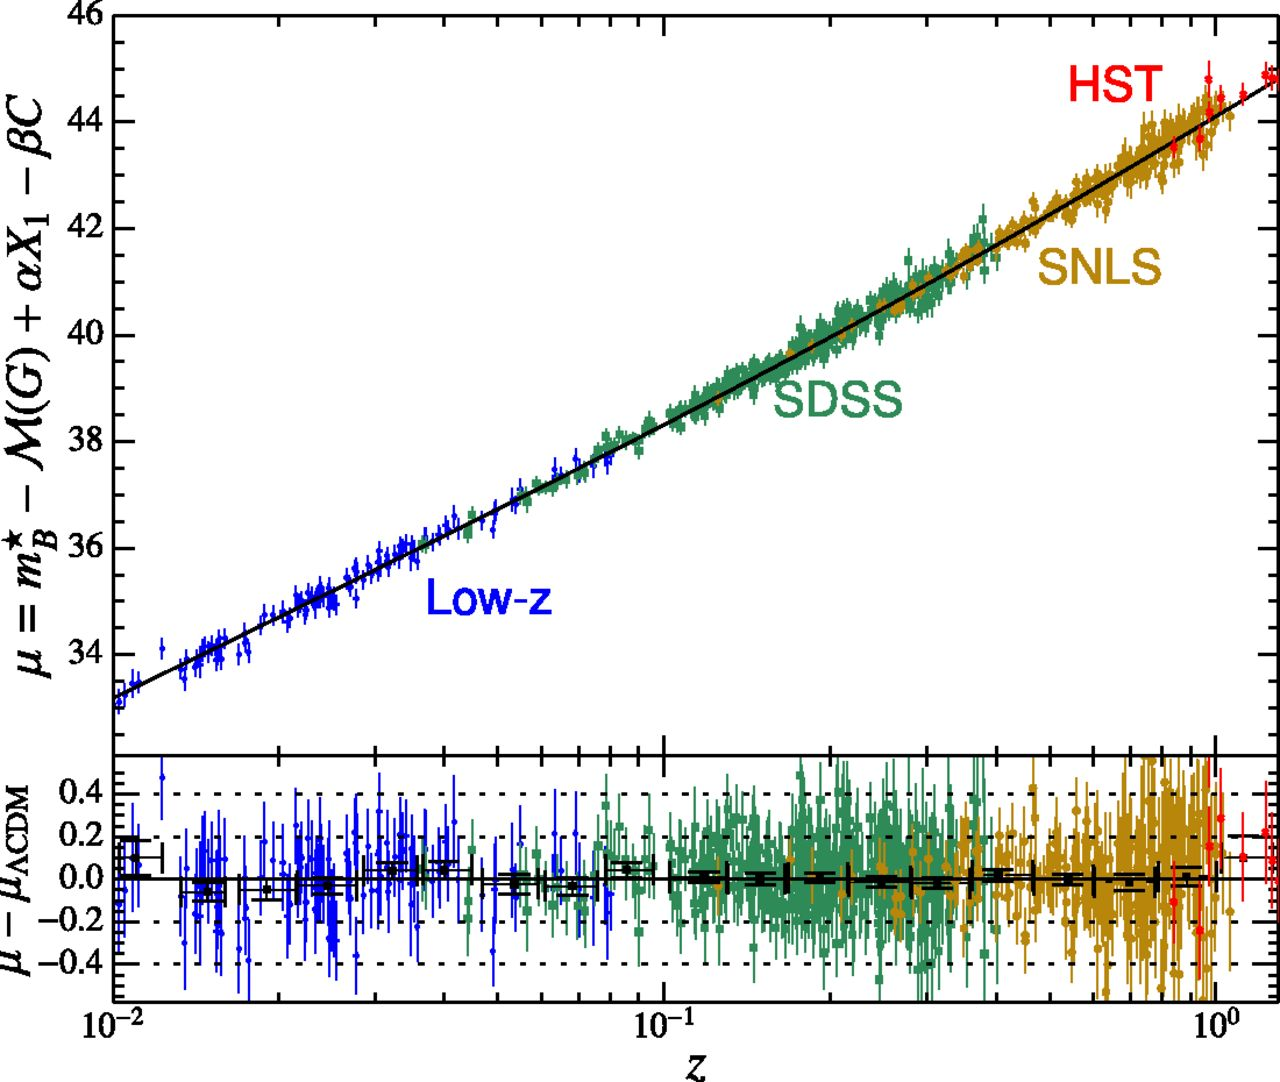
\includegraphics[width=.9\linewidth]{img/01/hubble_law.jpg} 
%        \caption[Loi de Hubble]{Loi de Hubble à partir d'observations actuelles. 
%        Figure extraite de \citep{2015PNAS..112.3173B}.
%%http://www.pnas.org/content/112/11/3173/F2.expansion.html
%%        Image ESO
%        }
% 		\label{fig:hubble_law}
%\end{figure}

La loi de Hubble est la relation entre la distance des galaxies $D$ et leur vitesse radiale d'éloignement $V$ : %est aujourd'hui appelée  et peux être résumé par :

\begin{equation}
V = H_0 D,
\end{equation}
où la constante de Hubble est aujourd'hui estimée à $H_0 = 67 \mathrm{ \left[ km.s^{-1}.Mpc^{-1} \right ] }$ \citep{planck_collaboration_planck_2016}.

%Conventionnellement, le sous script $0$ désigne le fait que la valeur de la variable qui lui est associé est celle prise aujourd'hui.
%Cette distinction est nécessaire car malgré son nom, la valeur de la constante de Hubble n'est pas constante dans le temps.
D'une manière plus générale la constante de Hubble représente la vitesse de variation relative de la distance entre deux points.
Elle s'exprime sous la forme:
\begin{equation}
H=\frac{1}{a} \frac{da}{dt} = \frac{\dot{a}}{a},
\end{equation}

où $a = a_{(t)}$ est le facteur d'expansion.
$a_0=1$ représente par définition la valeur de $a$ prise aujourd'hui.

%Comme la longueur d'une onde lumineuse est aussi impactée par l'expansion, 
Le redshift, s'exprime en fonction du facteur d'expansion de la manière suivante:
\begin{equation}
z= \frac{1}{a}-1
\end{equation}

\subsection{Équations de Friedmann}
\label{sec:friedman}

Les observations de Hubble ont permises de confirmer ce qui avait été pressentis par \cite{1916AnP...354..769E} plus d'une décennie plus tôt, lorsqu'il introduisit théoriquement le concept d'expansion de l'Univers. 
La théorie de la relativité générale introduit la célèbre equation de champ décrivant le lien entre densité d'énergie et déformation de l'espace-temps:

%Equation d'Einstein 
%http://cdsads.u-strasbg.fr/abs/1915SPAW.......844E
\begin{equation}
R_{\mu\nu} - \frac{1}{2} g_{\mu\nu}R + \Lambda g_{\mu\nu}  = \kappa T_{\mu\nu}.
\label{eq:einstein}
\end{equation} 

Dans cette équation apparaît le terme $\Lambda$ (de $\Lambda$CDM), appelée \textit{constante cosmologique}, et également :
%Cette constante représente mathématiquement le fait que l'espace-temps peut être en expansion ou en contraction.
$R_{\mu \nu}$ le tenseur de Ricci, $R$ la courbure scalaire, $g_{\mu \nu}$ le tenseur métrique, $T_{\mu \nu }$ le tenseur énergie-impulsion et $\kappa$ la constante d'Einstein.

%Metrique de Friedmann-Lemaître-Robertson-Walker (FLRW)

Quelques années plus tard, Alexandre Friedmann entreprend de trouver des solutions exactes à l'équation d'Einstein en l'appliquant a un Univers homogène et isotrope \citep{1922ZPhy...10..377F}.
Il arrive à ce système d'équations indépendantes permettant de modéliser l'Univers dans son ensemble :

%Recriture de l equation d'Einstein en considerant un univers homogene et isotrope.
% 
%Alexandre Friedmann Über die Krümmung des Raumes, Zeitschrift für Physik 10, 377-386 (1922). 
%Première écriture des équations de Friedmann, dans le cas d'une coubure spatiale positive. http://cdsads.u-strasbg.fr/abs/1922ZPhy...10..377F 
%
%(de) Alexandre Friedmann, Über die Möglichkeit einer Welt mit konstanter negativer Krümmung des Raumes, Zeitschrift für Physik 21 326–332 (1924). 
%Écriture des équations de Friedmann dans le cas d'une courbure spatiale négative. 
% 
%univers de Friedmann-Lemaître-Robertson-Walker  
%http://dictionnaire.sensagent.leparisien.fr/%C3%89quations%20de%20Friedmann/fr-fr/
 
%Équations de Friedmann : 

\begin{equation}
3 \left( \frac{H^2}{c^2} +\frac{K}{a^2} \right) = \frac{8 \pi G }{c^2} \rho
\label{eq:friedman1}
\end{equation}

\begin{equation}
-2 \frac{ \dot{H}}{c^2} -3 \frac{H^2}{c^2} -\frac{K}{a^2} = \frac{8 \pi G }{c^4 P}
\label{eq:friedman2}
\end{equation}

L'équation \ref{eq:friedman1} relie le taux d'expansion H, la courbure spatiale K et le facteur d'échelle a à la densité d'énergie $\rho$.
L'équation \ref{eq:friedman2} relie la pression P à la dérivée temporelle du taux d'expansion.
 
  
En manipulant l'équation \ref{eq:friedman1} il est possible de montrer que :
% cf 
% http://dictionnaire.sensagent.leparisien.fr/%C3%89quations%20de%20Friedmann/fr-fr/
% https://en.wikipedia.org/wiki/Friedmann_equations
% pour la demonstration

%TODO introduire les differents fluides cosmologiques

\begin{equation}
H = \frac{\dot{a}}{a} = H_0 \sqrt{ \Omega_{r,0} a^{-4} +  \Omega_{M,0} a^{-3} + \Omega_{K,0}a^{-2} + \Omega_{\Lambda,0}  } 
\label{eq:scale_t}
\end{equation}


\begin{figure}
        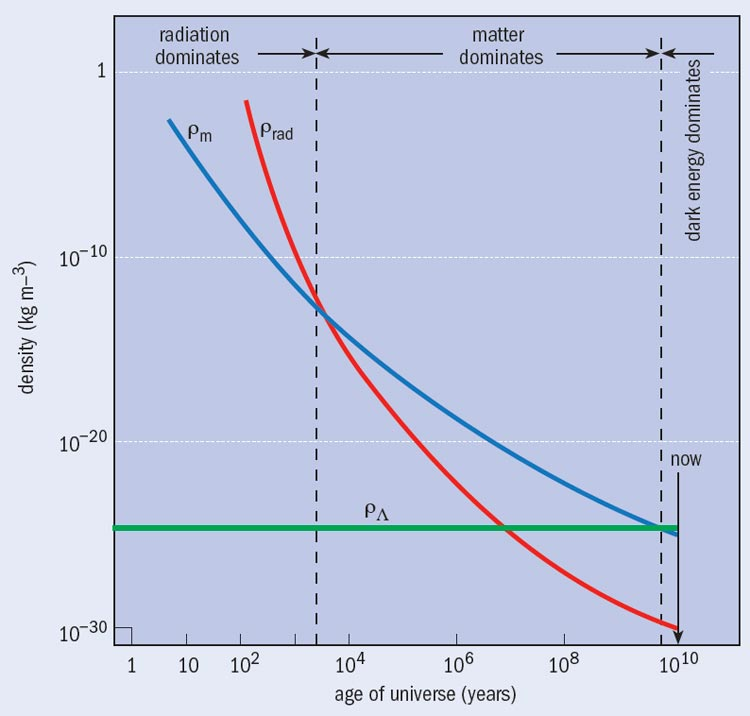
\includegraphics[width=.9\linewidth]{img/01/dark4.jpg} 
        \caption[Densités d'énergies]{Importance respective des différentes densité d'énergie en fonction de l'age de l'Univers (et donc de sa taille). Image extraite de \citep{2005univ.book.....F}
 		\label{fig:cosmoparamt} }
\end{figure}


Où les paramètres $\Omega_{i,0}$ représentent la densité d'énergie associée aux différents constituants, 
\begin{equation}
 \Omega_{i,0} = \frac{\rho_{i,0}}{\rho_{c,0}},
 \end{equation}

en fonction de la densité critique de l'Univers:

\begin{equation}
\rho_{c,0} = \frac{3H_0^2}{8\pi G}
 \end{equation}
Nous verrons dans la partie dédiée à la détermination des paramètres cosmologiques (cf Sec \ref{cosmoparam}) que les mesures actuelles sont en faveur d'un Univers plat (sans courbure).
Ce qui s'exprime par $\Omega_{K,0} = 0$ et $\Omega_{\lambda,0} +  \Omega_{M,0} + \Omega_{r,0} =1$.
La valeur de $\rho_c$ est déterminée avec l'équation \ref{eq:friedman1}, en considérant un Univers plat et statique ($\Lambda=0$).

\paragraph{$\Omega_{M,0}$} est le paramètre de densité d'énergie associée à la matière. % (matière noire que nous introduiront dans la suite et la matière baryonique)
Par simple effet de dilution, cette densité décroît avec le cube du facteur d'expansion.
Un Univers dominée par cette énergie est nommé "Univers poussière".
%C'est le cas actuellement.

\paragraph{$\Omega_{r,0}$} représente le paramètre de densité d'énergie relativiste.
La densité de photon décroît avec le cube du facteur d'expansion, mais du fait de l'allongement de la longueur d'onde avec $a$, la densité d'énergie associée au rayonnement décroît avec la puissance $4$ de $a$.
Un Univers dominée par cette énergie est nommé "Univers lumière".
%Cette approximation est valable pour un Univers majoritairement remplis de matière relativiste.
%C'était le cas avant l’émission du fond diffus cosmologique.

\paragraph{$\Omega_{\Lambda,0}$} est le paramètre de densité d’énergie du vide.
Cette énergie est associée à la constante cosmologique et à l'expansion de l'Univers et est constante dans le temps.

\paragraph{$\Omega_{K,0}$} est le paramètre de densité de courbure spatiale ou la densité d'énergie associée a la courbure de l'espace.
Selon l’équation \ref{eq:einstein}, l'énergie peut courber l'espace, mais si l'espace possède une courbure intrinsèque, elle est équivalente à une densité d'énergie.
\begin{equation}
\Omega_{K,0} = 1 - \Omega_{r,0} - \Omega_{M,0} - \Omega_{\lambda,0} 
\end{equation}

Comme ces densités d'énergies sont liées au facteur d'expansion, celles-ci évoluent avec le temps (cf Fig. \ref{fig:cosmoparamt}) est dominent à différentes époques,

\begin{figure}
        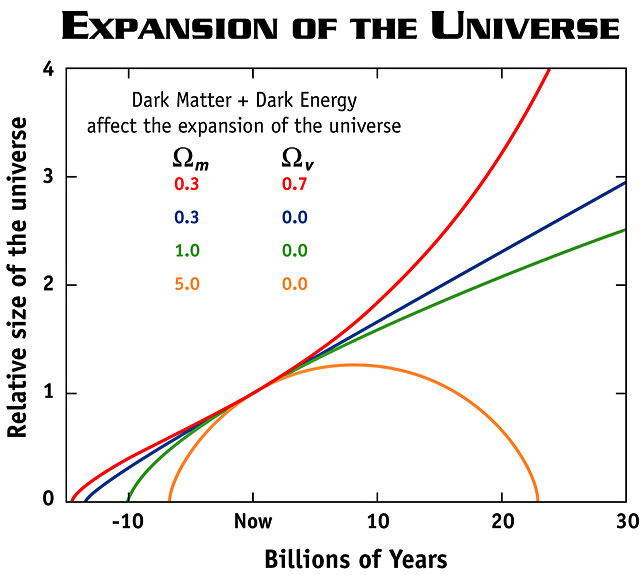
\includegraphics[width=.9\linewidth]{img/01/scale_t.jpg} 
        \caption[Taille de l'Univers]{Taille de l'Univers en fonction du temps pour différents paramètres cosmologiques.
		Image \href{https://map.gsfc.nasa.gov/universe/bb_concepts_exp.html}{NASA/WMAP Science Team}.
 		\label{fig:scale_t}}
\end{figure}

En intégrant l’équation \ref{eq:scale_t}, il est possible de déterminer l'évolution de la taille de l'Univers en fonction de la densité respectives de ses différents constituants.
La figure \ref{fig:scale_t} présente quelques évolutions possibles.
%Toutes les courbes passent par le point (Now,1) car par définition $a_0 = 1$.
%TODO expliquer cette histoire de tangente
%Toutes les courbes ont la même tangente au point (Now,1) du fait que $\Omega_{K,0}=0$
%TODO dire que nous somme la courbe rouge
Nous observons ici que la valeur des paramètres cosmologique contraint l'age actuel de l'Univers (le point où la courbe passe l'axe horizontal).
%La valeur des paramètres contraint aussi l'avenir de l'Univers.
%Par exemple, la courbe orange représente un Univers dit fermé.
%Ce type d'Univers est voué à s'effondrer sur lui même à cause de la gravité de la matière qu'il contient.
%A l'inverse, la courbe rouge représente un Univers dit ouvert.
%La gravitation n'est pas suffisante pour contrer l'expansion, et ce type d'Univers est voué a grandir indéfiniment.
%TODO dire que nous somme dans la courbe rouge
%\cite{2003PhT....56d..53P}

Le scénario actuellement admis est en faveur d'un Univers en accélération (courbe rouge).
L'accélération de l'expansion de l'univers a été découverte à la fin du XXème siècle par 2 équipes simultanément, chacune ayant reçue le prix Nobel en 2011 :
\begin{itemize}
\item  High-Z supernovae search team \citep{1998AJ....116.1009R} %http://cdsads.u-strasbg.fr/abs/1998AJ....116.1009R
\item  Supernova Cosmology Project \citep{1999ApJ...517..565P} % http://cdsads.u-strasbg.fr/abs/1999ApJ...517..565P
\end{itemize}

%\subsection{Énergie noire}
%\label{sec:dark_egy}
%
%%Dans un Univers, ou seule la gravité agit a grandes échelles, l'expansion ne peux que décélérer.
%
%Si nous avons vu que la taille de l'Univers évolue avec le temps, il reste la question de l'accélération de cette évolution.
%Si l'on considère que l'univers s'étend suite à une impulsion initiale (cf section \ref{sec:BB}), et que la gravité est la seule force qui agit à grande échelle, l'expansion devrait décélérée.
%%En effet comme la gravité est une force purement attractive, elle agit comme un ressort qui devrait ramener toute la masse à l'origine (scénario de la courbe orange sur la figure \ref{fig:scale_t}, ou la courbe retombe sur l'axe horizontal signifiant que la taille de l'univers tend à nouveau vers zero).
%Or ce n'est pas ce qui est observé: l'accélération de l'expansion de l'univers a été découverte a la fin du XXème siècle par 2 équipes simultanément, chacune aillant reçu le prix Nobel en 2011 :
%\begin{itemize}
%\item  High-Z supernovae search team \citep{1998AJ....116.1009R} %http://cdsads.u-strasbg.fr/abs/1998AJ....116.1009R
%\item  Supernova Cosmology Project \citep{1999ApJ...517..565P} % http://cdsads.u-strasbg.fr/abs/1999ApJ...517..565P
%\end{itemize}
%
%L'accélération de l'expansion de l'Univers pose un problème majeur.
%Il est établi depuis les travaux de Newton que pour accélérer une masse une force est nécessaire.
%Or nous ne disposons actuellement d'aucune théorie permettant d'expliquer cette force répulsive.
%Il a fallu seulement quelques mois après cette découverte pour qu’apparaisse pour la première fois la mention d'énergie noire \citep{1999PhRvD..60h1301H}.
%
%%échelle gigaparsec\\
%%Facteur d'expansion


\clearpage
\section{Le modèle du Big-bang}
\label{sec:BB}
%le big bang\\
%l'inflation\\
%la nucléosynthèse\\
%le CMB\\
%la reionization

Une fois établi que les galaxies s'éloignent de nous dans toutes les directions, plusieurs constats s'imposent.
Premièrement, en remontant le temps elles devaient être plus proches les unes des autres, et en poussant ce constat à l’extrême, à un certain instant dans l'histoire de l'Univers, toute la matière était extrêmement dense.
\cite{1927ASSB...47...49L} propose une théorie de l'atome primitif.
Cette singularité a été baptisée Big-bang et donne son nom au modèle cosmologique actuel.

%\subsection{Température de l'Univers}
%
%Il existe un lien direct entre la taille de l'Univers et sa température.
%Dans la conception actuelle de l'Univers, celui ci est par définition l'ensemble de ce qui existe, il ne lui est pas possible d'échanger de l’énergie avec l’extérieur : c'est donc un système isolé adiabatique.
%Or, la thermodynamique nous dit qu'il existe une relation entre le volume et la température d'un tel système : la température (la densité d'énergie interne) diminue au fur et à mesure que l'Univers se dilate.
%Plus l'on se rapproche temporellement du BigBang, plus l'Univers est dense et chaud.

\subsection{Nucléosynthèse primordiale}
\label{sec:nucleosynthese_primordiale}
%Dans le modèle du Big Bang, le début de l'Univers est suivis par une phase d'expansion rapide appelé inflation.
Après le Big-bang, l'Univers est suffisamment chaud pour présenter une soupe de particules élémentaires (quarks, gluons, leptons) qui vont former en se refroidissant les premiers protons et neutrons, qui vont à leur tour s'assembler pour former les premiers noyaux atomiques.
La théorie de la nucléosynthèse primordiale a été présentée par \citep{PhysRev.73.803} dans un article surnommé $\alpha \beta \gamma$ en référence aux initiales des noms de ses auteurs.
Cette théorie permet d'expliquer avec precision l'abondance observée des différents atomes présent dans l'Univers.
Il est aujourd'hui admis que l'abondance en masse de l'Univers est : 

\begin{itemize}
\item 73,9\% d’hydrogène,
\item 24\% d’hélium,
\item et 2.1\% de l'intégralité des autres éléments du tableau périodique (nous nommerons ces éléments "métaux" par convention).
\end{itemize}

L'hydrogène est largement majoritaire et l'hélium et les métaux seront négligés dans la suite de cette étude.

\subsection{Le fond diffus cosmologique}
\label{sec:CMB}

Tôt dans l'histoire de l'Univers, les noyaux atomiques sont découplés des électrons et l'Univers est dans un état ionisé. % correspondant à un plasma proche de celui que l'on peut trouver dans une étoile.
Il faudra attendre $\approx 380 000$ ans pour que la température diminue suffisamment pour permettre l'apparition des premiers atomes neutres.
Cette période est appelée "époque de recombinaison" (voir \cite{2009AN....330..657S} pour plus d'informations sur le sujet) et a donnée lieu à l'émission du fond diffus cosmologique ou \ac{CMB}.
Durant cette transition, l'Univers a connu un changement d'état majeur puisque celui ci est passé d'un état globalement ionisé à un état globalement neutre.
%Comme nous venons de le voir, l’émission du \ac{CMB} marque la transition entre deux états distincts de l'Univers.
Robert Herman et Ralph Alpher ont été les premiers à proposer l’existence du \ac{CMB} en 1948 avant même sa découverte.
%Le \ac{CMB} étant la plus ancienne lumière que nous pouvons observer, il contient actuellement l'information que nous pouvons obtenir sur l'état de l'Univers lorsqu'il était le plus jeune possible.
%
%\subsection{Surface de dernière diffusion}
%
%En raison du grand nombre d'électrons libres avant la recombinaison, la lumière était soumise à un grand nombre de diffusions.
%À la manière de la surface d'une étoile, où nous ne voyons que les photons qui ont pu s’échapper de celle ci et non ceux qui ont été émis en son centre, nous ne pouvons pas observer de lumière émise avant le \ac{CMB}.
%Le \ac{CMB} étant la plus ancienne lumière que nous pouvons observer, il contient actuellement l'information que nous pouvons obtenir sur l'état de l'Univers lorsqu'il était le plus jeune possible.

%La quête de l'état de l'Univers à ses début a commencé de manière fortuite en 1964 quand Penzias et Willson ont observé, lors de travaux sur un nouveau type d’antenne radio, un signal radio inexpliqué.
%Ce signal était constant et extrêmement homogène. 
%(l'anisotropie du CMB est remis en cause recement 
%http://www.ca-se-passe-la-haut.fr/2013/09/lanisotropie-du-fond-diffus-cosmologique.html)
Penzias et Willson ont observé le \ac{CMB} en 1964 et obtiennent le prix Nobel en 1978 pour la \cite{PenziasWilsonNobel}.
Cette observation constitue un argument de poids en faveur de la théorie du Big-bang et une série de missions spatiales lui ont été consacrées.
%dans le but d'améliorer les mesures faites sur le \ac{CMB}.

\begin{itemize}
\item 1989 - le satellite COsmic Background Explorer COBE 
\item 2001 - le satellite Wilkinson Microwave Anisotropy Probe WMAP
\item 2009 - le satellite Planck
\end{itemize}

%\subsection{Température}
%Le \ac{CMB} se présente sous la forme du corps noir à une température de T=2.73°K.
%La figure \ref{fig:cmb_thermal_spectrum} compare le spectre thermique observé à celui d'un corps noir théorique. 
%La correspondance est presque parfaite.
%
%Le \ac{CMB} a été émis lorsque l'Univers était à une température de $T \approx 3000$ K.
%Le signal reçu est donc redshifté d'un facteur $z\approx1100$ par rapport à celui émis lors de la recombinaison.
%
%\begin{figure}[htbp]
%        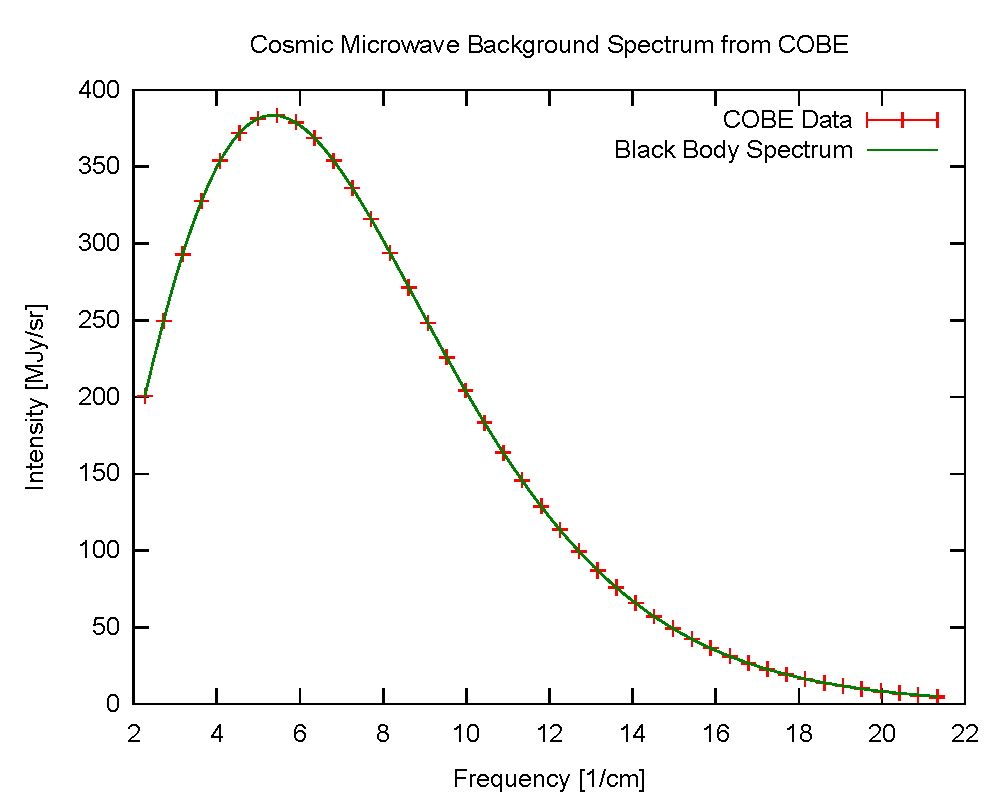
\includegraphics[width=.95\linewidth]{img/01/Cmbr.pdf} 
%        \caption[Température CMB]{Spectre thermique du \ac{CMB} vue par le satellite Cosmic Background Explorer (COBE). 
%        Image Wikipédia
% 		\label{fig:cmb_thermal_spectrum}}
%\end{figure}

Lors de sa découverte, le \ac{CMB} était considéré comme uniforme mais, John C. Mather et George F. Smoot ont conjointement obtenus le prix Nobel de physique en 2006 pour la \cite{CMBanisotropiesNobel} grâce aux observations réalisées par le satellite  COBE.
Ce léger défaut d'uniformité (de l'ordre de $10^{-5}$ en relatif) nous renseigne sur l’état de l'univers au moment de son émission.
Par la suite, les satellites WMAP et Planck ont grandement amélioré la précision des mesures des anisotropies du fond diffus (Fig. \ref{fig:cmb}).

\begin{figure}
%        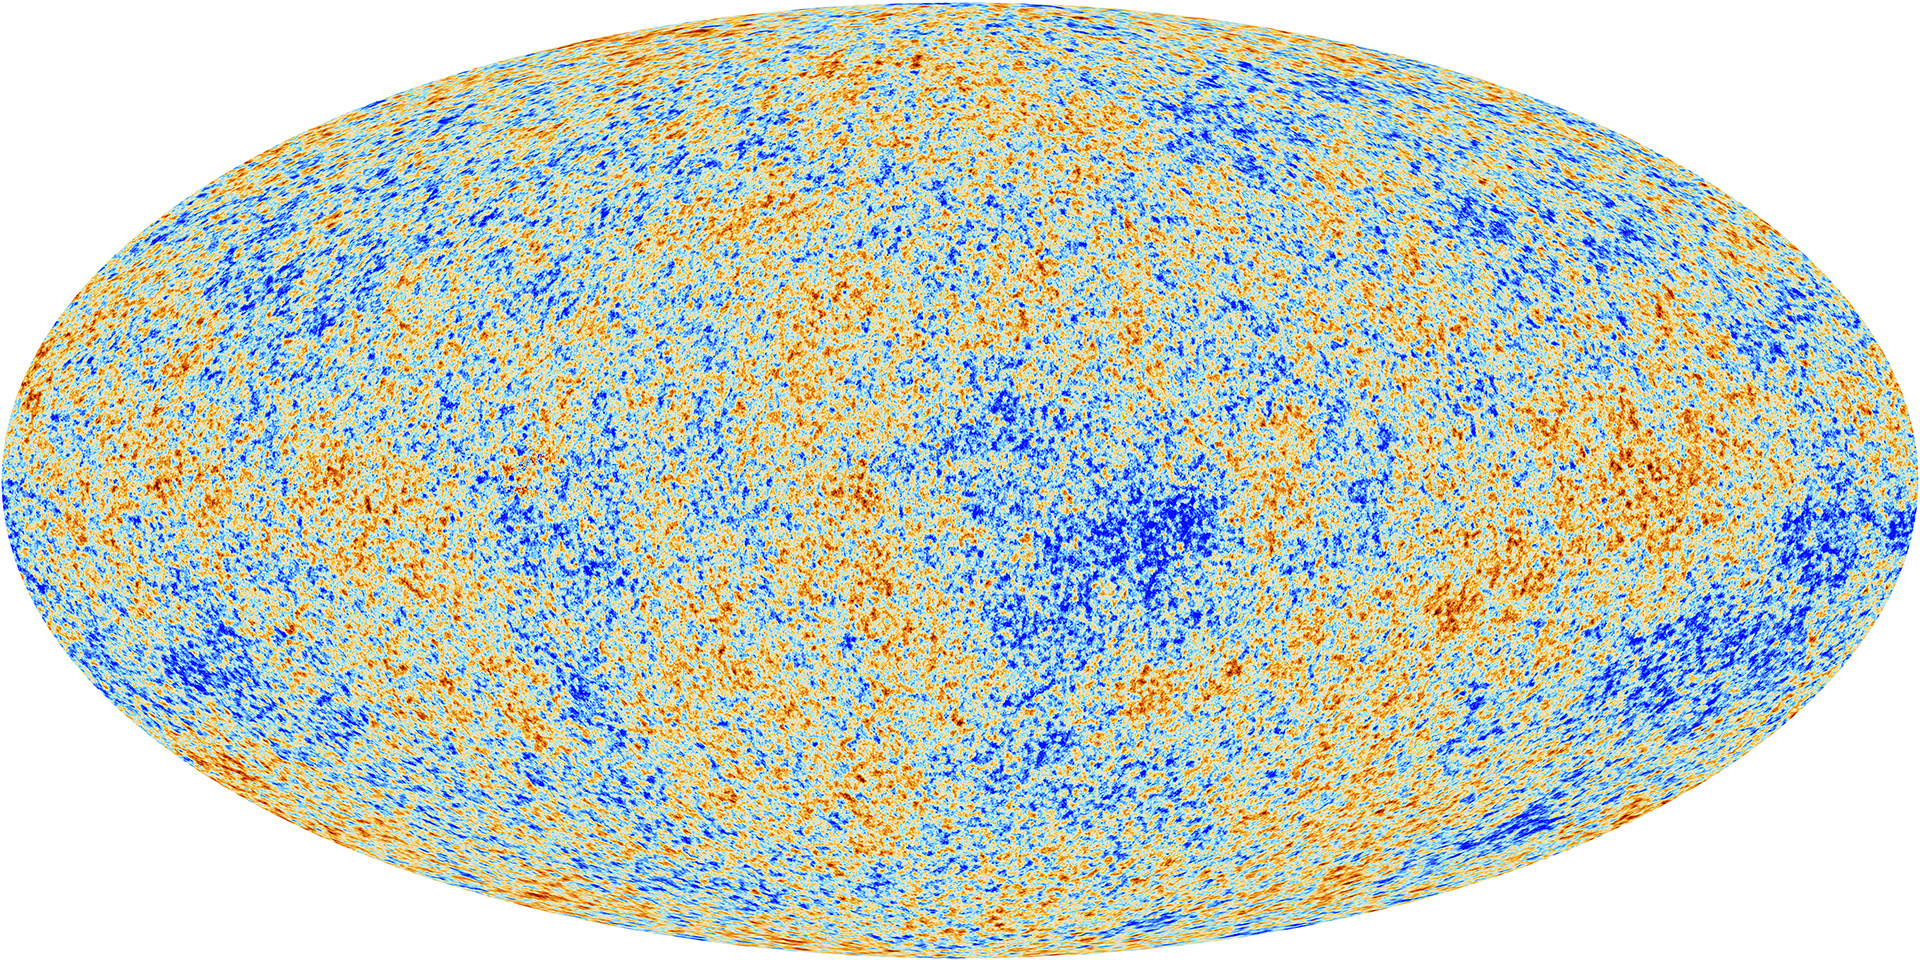
\includegraphics[height=.95\textheight]{img/01/CMB.jpeg} 
        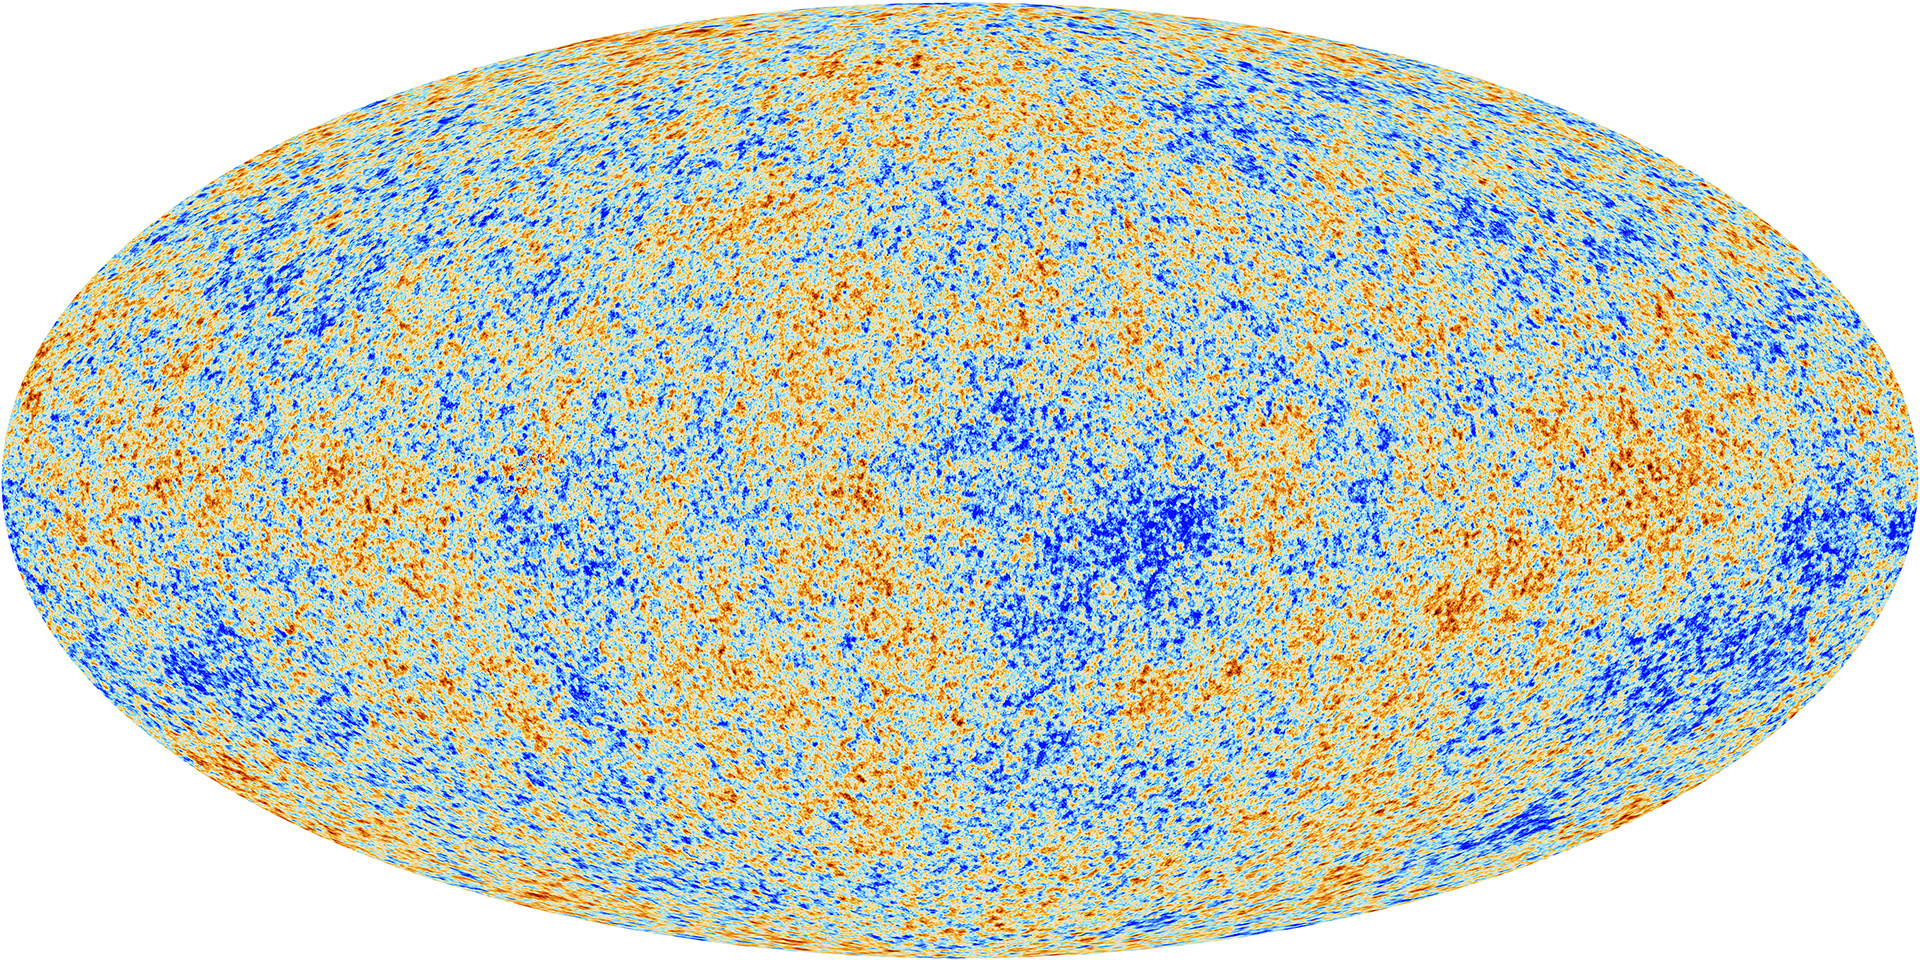
\includegraphics[width=0.95 \textwidth]{img/01/CMB.jpeg} 

        \caption[CMB]{Les fluctuations du \ac{CMB} vues par le satellite Planck. 
        Image ESA}
 		\label{fig:cmb}
\end{figure}

%Les anisotropies du \ac{CMB} sont étudiées en décomposant les fluctuations relatives de température en harmoniques sphériques.
%Un spectre de puissance, correspondant à la transformée de Fourrier de sa fonction de corrélation a deux points, caractéristique est obtenu (cf figure \ref{fig:cmb_power_spectrum}).

%%decomposition en multipoles
%%https://www.physicsforums.com/threads/can-someone-explain-angular-power-spectrum.309483/
%\begin{equation}
% \frac{\Delta T(\theta,\phi)}{T} = \sum_{l>0} \sum_{m=-l}^l a_{lm} Y(\theta,\phi)_{lm}
%\end{equation}
%
%avec : 
%
%\begin{equation}
%a_{lm}= \int d\Omega(\theta,\phi) \Delta T (\theta,\phi) Y(\theta,\phi)_{lm}
%\end{equation}
%
%%Fig\,\ref{fig:harmoniques_spheriques}
%%\begin{figure}[bth]
%%        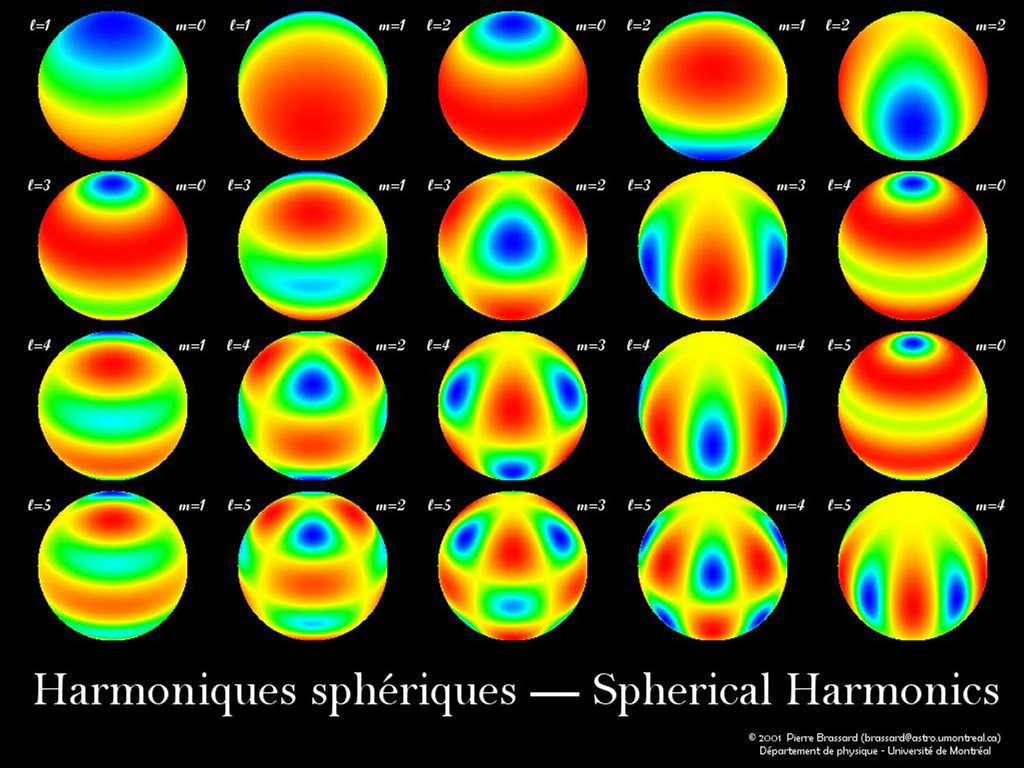
\includegraphics[width=.95\linewidth]{img/01/harmoniques_spheriques.jpeg} 
%%        \caption{
%%        représentation des $Y(\theta,\phi)_{lm}$
%% Pierre Brassard, université de Montréal 
%%%Spectre thermique du CMB vue par le satellite Cosmic Background Explorer (COBE). 
%%        Image Wikipédia}
%% 		\label{fig:harmoniques_spheriques}
%%\end{figure}
%
%\begin{equation}
%C_l = \frac{1}{2l+1} \sum_{m=-l}^l a_{lm} a_{lm}^*
%\end{equation}
%
%Et finalement, on obtient le spectre de puissance représenté Fig.\,\ref{fig:cmb_power_spectrum}:
%
%\begin{equation}
%D_l = \frac{l (l+1) C_l }{2 \pi} 
%\end{equation}


\begin{figure}
        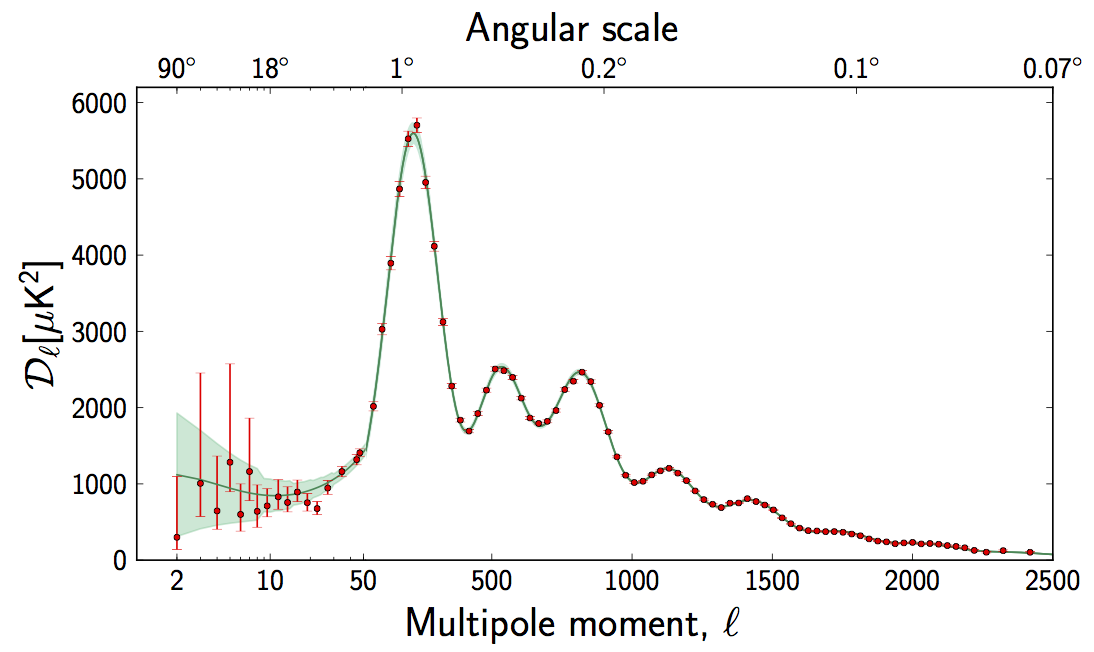
\includegraphics[width=.95\linewidth]{img/01/CMB_power_spectrum.png} 
        \caption[Spectre de puissance des fluctuation du CMB]{Spectre de puissance des fluctuation du \ac{CMB}.
        Image ESA}
 		\label{fig:cmb_power_spectrum}
\end{figure}

%Fig. \ref{fig:cmb_power_spectrum}

Le spectre de puissance du \ac{CMB} contient de l'information sur la distribution de la matière au moment de l'émission du \ac{CMB}, et ces fluctuations de température sont essentielles pour expliquer la formation des grandes structures observées aujourd'hui.
En effet, comme il existe un lien direct entre la température et la densité, il est possible de déterminer la distribution de matière à l'époque de l'émission de \ac{CMB}.
%les régions aillant une température légèrement plus élevées correspondent aux régions légèrement plus denses, et réciproquement. 
%Nous verrons plus tard (cf section \ref{sec:IC}) que cette distribution de matière à très haut redshift permet la génération des conditions initiales nécessaire pour effectuer des simulations.

\section{Le contenu de l'univers}
\label{cosmoparam}

\begin{figure}
        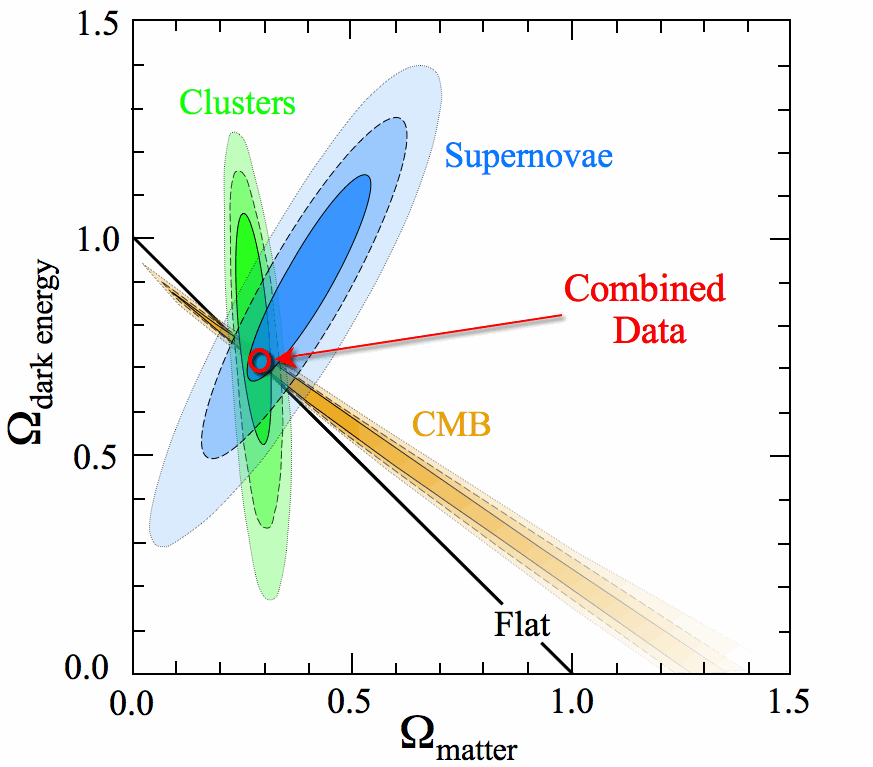
\includegraphics[width=.95\linewidth]{img/01/cosmoparam.png} 
        \caption[Determination des paramètres cosmologique]{Détermination des paramètres cosmologique a partir de différents observables. Figure extraite de \cite{2008ApJ...686..749K}}
 		\label{fig:cosmoparam}
\end{figure}


La distribution des fluctuations de densité n'est pas la seule information contenue dans le \ac{CMB}, nous verrons dans la prochaine section que se spectre contient également de l'information sur l'abondance des différents constituants de l'Univers.
%La première étape pour comprendre l'univers, est de déterminer ce qu'il contient, et quelles sont les physiques dominante à considérer, en fonction de ce que l'on cherche à étudier.
Il est possible de créer un modèle théorique du plasma primordial capable de prédire le spectre de puissance de l'émission de recombinaison.
En comparant le spectre de puissance théorique obtenu à celui du \ac{CMB} observé, il est possible de déterminer les paramètres libres du modèle par ajustement.
La figure \ref{fig:cmb_power_spectrum} représente la comparaison entre le meilleur ajustement actuel et les observations, 

La détermination des abondances respectives des différents constituants, utilise conjointement plusieurs observables.
%Chacune de ces observables va pouvoir être lier à un modèle disposant de plusieurs paramètres libres.
Les supernovæ considérées comme chandelle standard, suffisamment lointaines permettent d'obtenir de l'information sur l'accélération de l'expansion de l'Univers (un gamme de valeurs pour $\Omega_\Lambda$) (voir par exemple \cite{1999ApJ...517..565P} pour plus d'informations sur le sujet).
%Ou encore la distribution actuelles des galaxies, en partie reliquat des oscillations acoustiques dans le plasma primordial, permet de contraindre les paramètres cosmologique.
Ou encore l'abondance observée des amas de galaxies permettent de contraindre $\Omega_m$.

%A partir de différents observables,
%En recoupant les données obtenues a partir d'observations comme , 

%Le spectre de puissance du fond diffus cosmologique permet de déterminer les quantité respectives des différents constituants de l'univers.
%En recoupant ces données a d'autre observables, comme la distribution des amas de galaxies ou les supernovae lointaines, il est possible de contraindre les paramètres cosmologiques (Fig. \ref{fig:cosmoparam}).

Une représentation de ces différentes contraintes sur l'abondance des densités d'énergie noire et de matière est visible sur la figure \ref{fig:cosmoparam},
Ces paramètres de densités ne sont pas les seuls paramètre libres du modèle standard et une compilation de ces paramètres est présenté sur la figure \ref{fig:planck_parameters}.
Ces paramètres ont été obtenus par \cite{planck_collaboration_planck_2016} et sont actuellement les plus récents disponibles.

%A partir du spectre de puissance, on peut déterminer les différentes composantes de l'univers (paramètres cosmologique).
%univers infini, homogène, isotrope


%https://ned.ipac.caltech.edu/level5/Freedman2/Freed6.html


\begin{figure}
        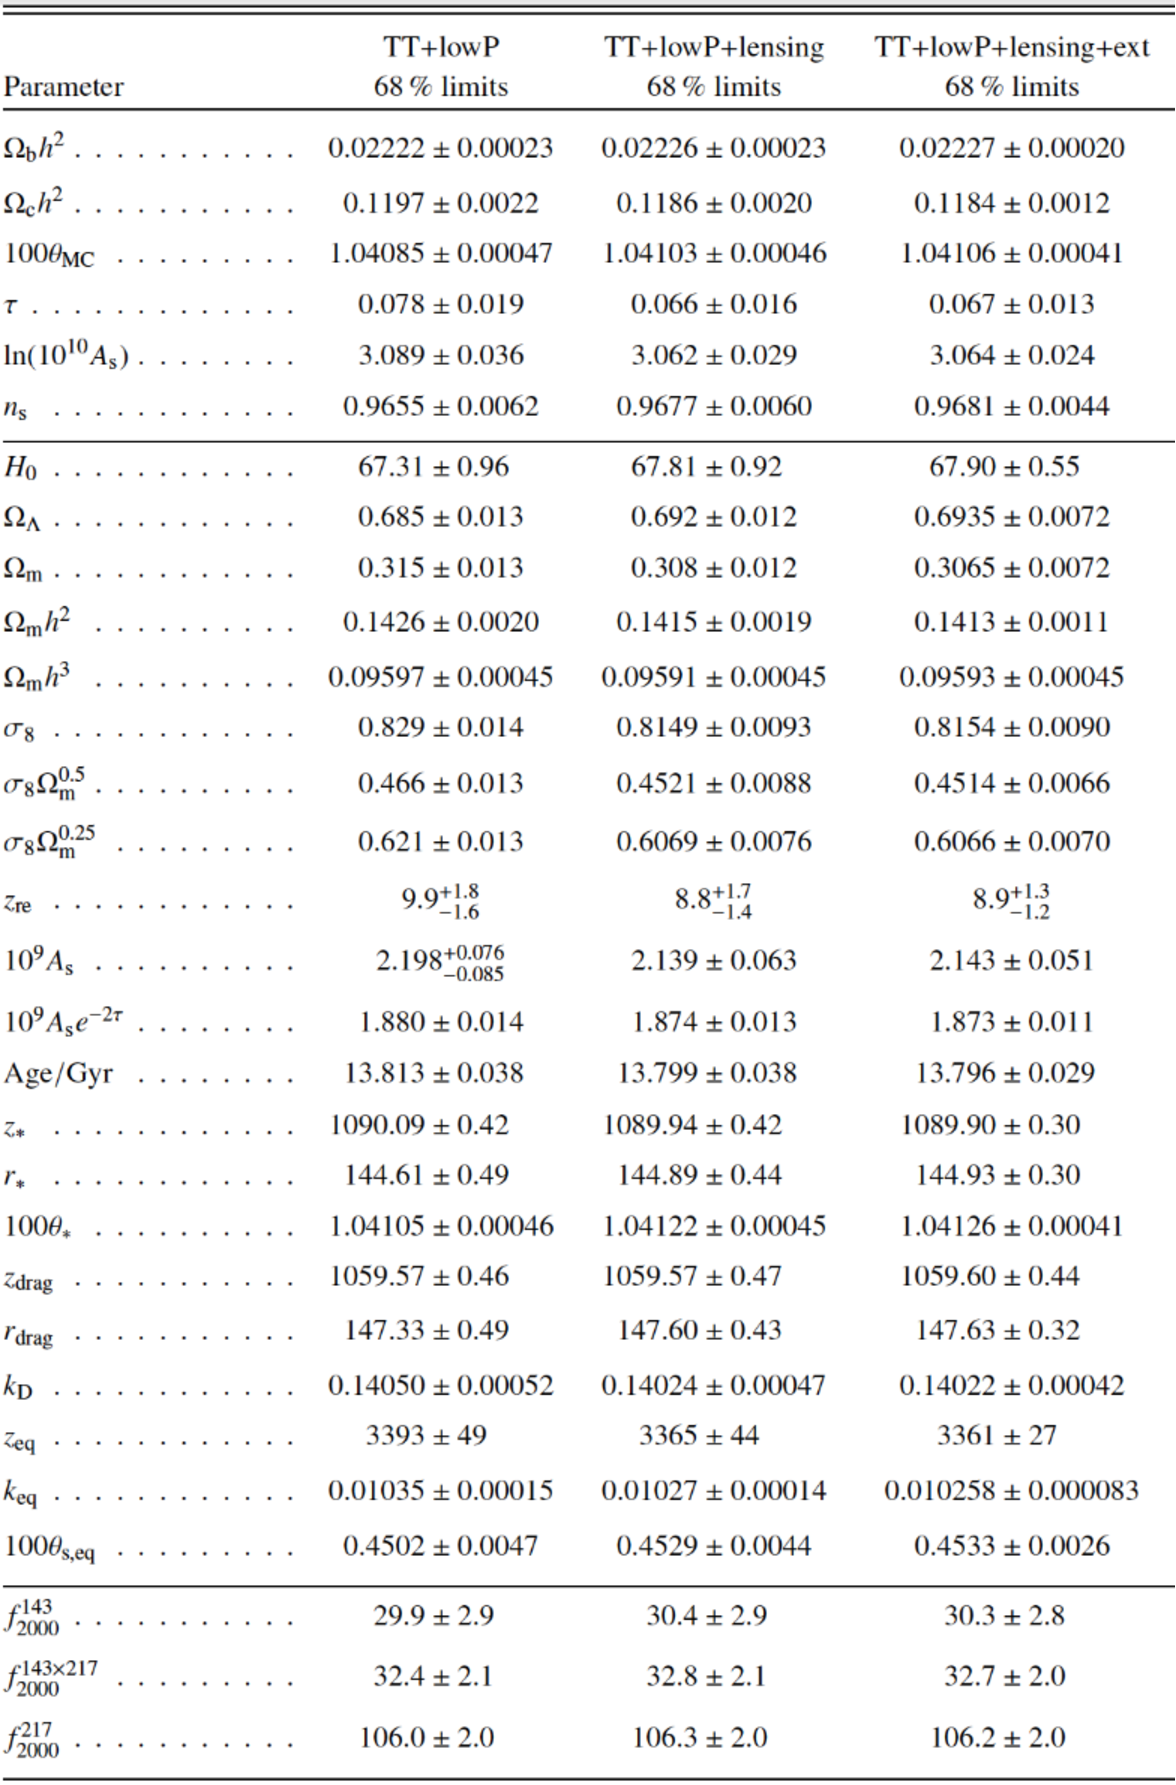
\includegraphics[width=.95\linewidth]{img/01/table_planck2.pdf} 
        \caption[Tables paramètres cosmologique]{Détermination des paramètres cosmologiques par \cite{planck_collaboration_planck_2016} }
 		\label{fig:planck_parameters}
\end{figure}
%
%
%
%\subsection{Énergie noire}
%Nous avons déjà abordé le sujet de l'énergie noire dans la section \ref{sec:dark_egy}.
%Avec une abondance relative de près de 70 \%, l'énergie noire est le principal constituant de l'Univers.
%Elle a été introduite pour expliquer l'accélération de l'expansion l'Univers.
%Elle contraint la distribution de matière sur les plus grandes échelles (de l'ordre du Giga parsec).
%Nous n'avons pas d'idée sur sa provenance mais des future missions comme EUCLID \citep{2016PhRvD..94l3515T} permettront d'obtenir plus d'information à son sujet.
%
%\subsection{Matière noire CDM}
%
%La matière noire est un vaste sujet.
%Le modèle $\Lambda$CDM nécessite une certaine quantité de matière pour expliquer les interactions gravitationnelles observées.
%Cette quantité de matière n'est pas en accord avec les observations réalisées sur la matière visible.
%Il a donc été nécessaire d’introduire une matière invisible appelée matière noire.
%La matière noire représente 26\% du bilan énergétique total et gouverne les échelles de l'ordre du Mega parsec.
%Elle est la principale source de gravitation et présente des propriétés non collisionnelles.
%
%Entre autres indications de la présence d'une matière non détectée, il y a:
%\begin{itemize}
%
%\item Les courbes de rotation des galaxies.
%Il est possible d’estimer la masse d'une galaxie à partir de sa luminosité (masse lumineuse).
%Il est également possible de déterminer sa masse en étudiant sa vitesse de rotation en fonction de son rayon (masse dynamique).
%La comparaison entre la masse dynamique et la masse lumineuse montre que les galaxies tournent plus vites que prévu et que la masse lumineuse est plus faible que la masse dynamique.
%
%\item Le bullet cluster.
%Il s'agit de la collision entre deux amas de galaxies dont les caractéristiques semblent actuellement présenter la meilleur piste en faveur de la présence de matière noire.
%
%\item Le spectre de puissance du \ac{CMB} (voir section \ref{sec:cmb_power_spectrum}), et plus particulièrement son troisième pic, est sensible au ratio matière/rayonnement et indique la présence de matière noire.
%
%\end{itemize}
%
%%\subsubsection{CMB}
%
%
%%\subsubsection{Bullet cluster}
%
%%echelle mega parsec\\
%%gouverne la gravité\\
%%non collisionnelle\\
%%
%%
%%\begin{figure}[bth]
%%        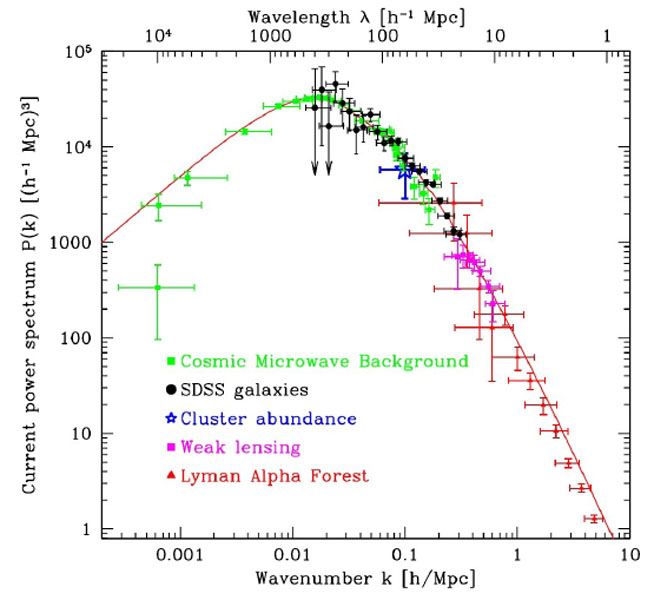
\includegraphics[width=.95\linewidth]{img/01/matter_power_spectrum.jpeg} 
%%        \caption{Spectre de puissance de distribution de la matière a grande échelle
%%        %http://adsabs.harvard.edu/cgi-bin/bib_query?2004PhRvD..69j3501T
%%        }
%% 		\label{fig:matter_power_spectrum}
%%\end{figure}
%
%\subsection{Baryon}
%
%Les baryons correspondent à la matière connue, avec laquelle la lumière interagis.
%Ils ne représentent qu'environ 5\% du bilan énergétique global.
%Les baryons interagissent également entre eux, et ont une physique collisionnelle.
%Leur introduction dans les simulations a été nécessaire lorsque l'on a commencer à étudier des échelles de l'ordre du kiloparsec et la formation stellaire.
%
%%echelle kilo parsec
%%collisionnelle
%%interagit avec la radiation
%%La matière visible
%
%\subsection{Radiation}
%
%La radiation ne représente aujourd'hui que $10^{-4}$ de l'énergie totale.
%Elle représente notre seul source d'information sur l'univers (Ce n'est plus le cas depuis la récente découverte des ondes gravitationnelles) %TODO ref
%Elle est centrale dans le processus de réionisation.
%La radiation est capable d'impacter a la fois les petites échelles de l'ordre du parsec (en interagissant avec la formation stellaire)
%et aux grandes échelles de l'ordre de la centaine de Méga parsec en changeant les propriétés optiques de l'\ac{IGM}.
%
%%A la fois les grandes échelles et les petites.
%%Son introduction dans les simulations 
%
%%seulement E>13.6 eV
%
%
%%\subsection{Bilan}
%%
%%plot en camembert avec les différents constituants
%
%%perturbation lineaires:
%%https://ned.ipac.caltech.edu/level5/Sept11/Norman/Norman2.html


\section{Formation des structures}
\label{sec:formationgalaxie}

%Nous avons vu dans la partie dédiée au fond diffus cosmologique que  
L'Univers n'était pas parfaitement homogène lors de l'émission du \ac{CMB} et la croissance de ces perturbations primordiales va mener, sous l'effet de la lutte entre l'expansion et la gravitation, à un effondrement de la matière sur elle même \citep{1968ApJ...151..459S}.
%C'est dans ces surdensités locales que vont se former les premières galaxies.
La première étape à la formation d'une galaxie est donc l'effondrement d'une surdensité et cet effondrement est largement dominé par la matière noire \citep{1985ApJ...292..371D}.

Pour qu'une surdensité s'effondre, il faut que sa masse soit supérieure à la masse de Jeans.
Après le découplage matière/rayonnement cette masse chute brutalement \citep{2010gfe..book.....M}, autorisant la contraction de structures de $M \approx 10^6 M_\odot$.
Cette masse évolue en fonction du redshift \citep{2016PhR...645....1B} : 
\begin{equation}
M_j \approx 6 \cdot 10 ^3 \left( \frac{1+z}{10} \right)^{3/2} M_\odot
\end{equation}


Pour étudier la croissance des fluctuations primordiales on utilisera la théorie des perturbations linéaires.
On remplacera la densité par la densité perturbée $\rho(x) = <\rho> + \delta(x)$ où $\delta$ sera appelé le contraste de densité :

\begin{equation}
\delta(x) = \frac{\rho(x)}{<\rho>} -1.
\end{equation}

On cherchera alors une solution des équations régissant le fluide primordial, en utilisant l'approximation au premier ordre \citep{1999coph.book.....P}.
Cette approche permet de prédire les oscillations acoustiques des baryons ou Baryonic Acoustic Oscillations (BAO) observées dans la distribution des galaxies \citep{2005ApJ...633..560E}.
Pour rester dans le domaine linéaire, le contraste doit rester faible et représenter l'homogénéité de l'Univers aux grandes échelles.

A partir de cette solution perturbée, \cite{1970A&A.....5...84Z} propose une approche dynamique (voir \cite{2014MNRAS.439.3630W} pour une revue récente) permettant la génération de conditions initiales utilisées dans les simulations numériques.
En effet, arrivée à la fin du régime linéaire, il devient nécessaire d'utiliser des simulations numériques pour étudier la formation des structures en détails.
Les simulations de croissances des structures réalisées avec les considérations exposées dans cette section donnent une excellente similarité avec les observations (voir figure \ref{fig:sdss}).

\begin{figure}
        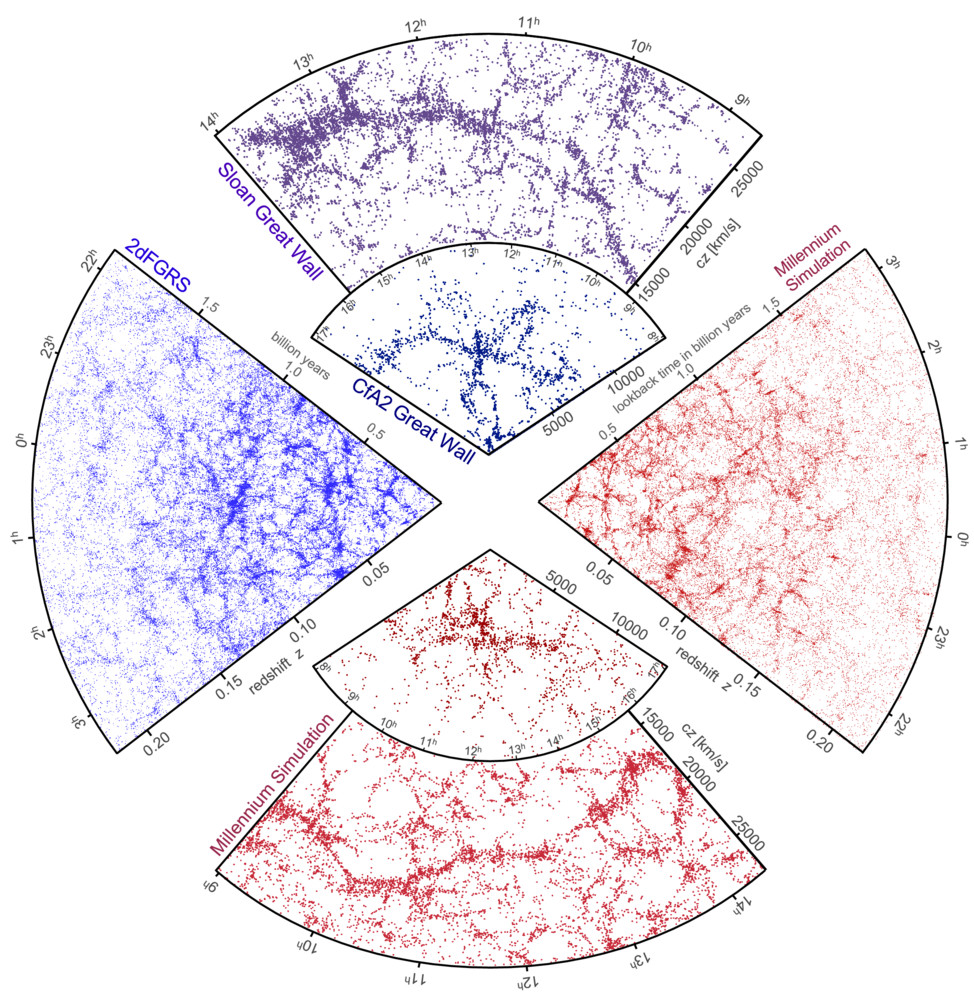
\includegraphics[width=.95\linewidth]{img/02/sdss_millenium.jpeg} 
        \caption[SDSS - Millennium]{Comparaison entre les structures à grandes échelles observées par le SDSS (en bleu) et celles reproduite dans la simulation Millennium \citep{2005Natur.435..629S} (en rouge).
%http://wwwmpa.mpa-garching.mpg.de/millennium/
 		\label{fig:sdss}}
\end{figure}

\clearpage
Malgré la forte non-linéarité de la croissance des structures, il est tout de même possible de faire quelques prescriptions analytiques.
Notamment en considérant le cas idéal de l'effondrement d'une surdensité sphérique dans le cas d'un Univers en expansion.
En cherchant les solutions de:
\begin{equation}
\frac{d^2r}{dt^2} = -\frac{GM}{r^2} + \frac{\Lambda}{3}r, 
\end{equation}
ou $M$ est la masse contenue au sein d'une coquille sphérique de rayon $r$, et en y appliquant le théorème du Viriel:
\begin{equation}
2T+U=0
\end{equation}
où $T$ est l'énergie cinétique et $U$ l'énergie interne, il est possible de déterminer $\Delta_{vir}$ la densité moyenne des structure en effondrement \citep{2010gfe..book.....M}.
Dans le cas d'un Univers plat cette sur densité s'exprime :
\begin{equation}
\Delta_{vir} \approx (18 \pi ^2 + 82 (\Omega_m-1) - 39 (\Omega_m-1)^2)/ \Omega_m
\end{equation}

En pratique $\Delta_{vir}$ est de l'ordre de $\approx 200 \bar{\rho}$.
Dans la suite on considérera $R_{200}$ le rayon d'une surdensité de $200 \bar{\rho}$ comme une approximation du rayon de Viriel $R_{vir}$:
\begin{equation}
R_{200} \approx R_{vir}
\end{equation}

Cet effondrement va mener à la formation de structures majoritairement composée de matière noire.
Ces halos de matière noire vont former des puits de potentiel et entraîner les baryons qui formerons les galaxies.

Ces halos auront différentes masses en fonction des fluctuation de densités initiales
On définis le spectre de puissance des fluctuation de densité comme :

\begin{equation}
P(k) = \left< | \delta(x) |^2 \right>
\end{equation}

En analysant la variance de $P(k)$, \cite{1974ApJ...187..425P} ont déterminé $n$ le nombre halos ayant une masse comprissent en $M$ et $M+dM$
\begin{equation}
\frac{dn_{(M,t)}}{dM} = \sqrt{\frac{2}{\pi}} \left| \frac{\rho_0}{M^2} \right| \frac{d ln \sigma}{d ln M} \frac{\delta_0}{\sigma_{(M)}} exp \left[ - \frac{\delta_{0c}^2}{2\sigma_{(M)}^2} \right].
\end{equation}

Cette grandeur est appelée fonction de masse des halos ou \ac{HMF} et est représentée sur la figure \ref{fig:hmfpress}.

\begin{figure}
        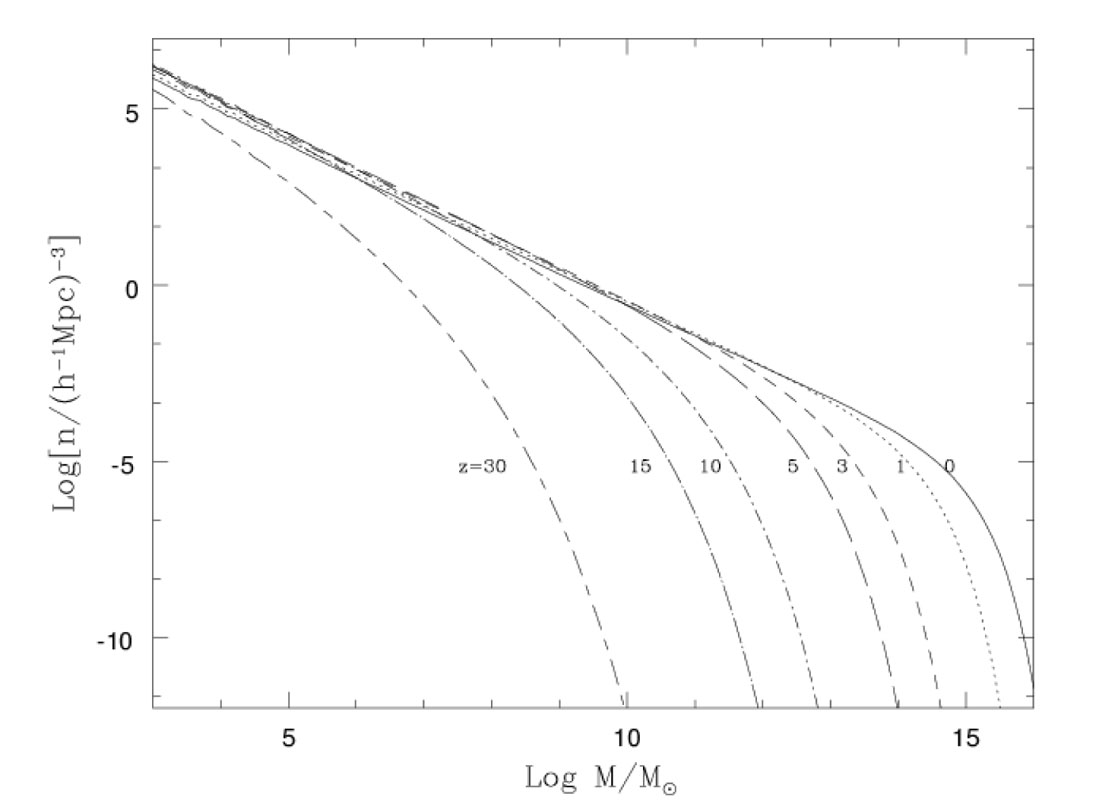
\includegraphics[width=.95\linewidth]{img/01/press.jpg} 
        \caption[HMF théorique]{Fonctions de masses théoriques de halos déterminées par \cite{1974ApJ...187..425P} à différents redshift.
        Image issue de \href{ned.ipac.caltech.edu}{ned.ipac.caltech.edu}
 		\label{fig:hmfpress}}
\end{figure}

%\chapter{La reionisation} 
\label{sec:introreio}
%réionisation et non rayonnisation!
%\section{Observation -> la reionization}
%%\section{Théorie -> La reionization}
%
%
%Qu'est ce que c'est?
%
%fin des âges sombres
%apparition des première sources de rayonnement
%Pourquoi étudier la réionisation
%
%Dernier processus impactant l'ensemble de l'univers.
%Importance pour le "missing satellite problem"
%%le manque d'observations
%%la difficulté des observations

Nous avons vu dans le chapitre précédent que lors de la recombinaison, l'Univers est passé d'un état globalement ionisé à un état globalement neutre.
%De cette transition, qui a eu lieu a environ 380000 ans après le Bigbang, en a résulté L’émission du CMB.
Suite a cette étape, l'univers était alors très homogène et ne disposait pas de source lumineuse, c'était les "ages sombres".

Sa dynamique était régie essentiellement par la lutte entre l'expansion et la gravitation et la compétition entre ces deux forces, couplée à de très légères perturbations a menée a l'effondrement de certaines certaines parties.
Il faudra alors attendre plusieurs centaine de million d'année pour voir apparaître des surdensité de gaz suffisamment compactes pour former les première étoiles.
Ces premières sources lumineuses ont émis un puissant rayonnement ionisant qui a a nouveau séparé les protons et les électron formé lors de la recombinaison.
Il a fallut encore plusieurs centaine de million d'année pour que les première sources de rayonnement soient suffisamment nombreuses pour que leurs photons remplissent l'univers, et le fasse passer d'un état majoritairement neutre, a un état a nouveau majoritairement ionisé. 
Cette transition s'appelle l’époque de la réionisation.

%à l'apparition des premières des premières étoiles.
%L'Univers va alors subir un changement d'état majeur, puisque le rayonnement énergétique des premières étoiles va de nouveau ioniser le gaz.
%C'est l'époque de la réionisation.

%Du fait que l'univers était neutre, le rayonnement n’était pas en mesure de se propager librement.
%A la suite de l'émission du fond diffus cosmologique, commence une période appelée "les ages sombres".
%L'Univers est alors composé de gaz froid soumis principalement à deux forces : la gravité et l'expansion de l'Univers.
%Ces étoiles ont émis du rayonnement suffisamment énergétique pour arracher les électrons du gaz environnant.



L'objectif de cette section est de présenter les grandes lignes des principes physique qui ont eu lieu durant cette période.
Je présenterai également quelques des preuve observationnelles qui confirme que la réionisation a bien eu lieu.
%Dans cette section, je vais présenter quelques unes des preuve observationnelles de la réionisation. 

%Une des difficultés de l’étude de la période de réionisation est que celle si a eu lieu tôt dans l'histoire de l'univers lors de son premier milliard d'années.
%Cette distance temporelle impose de regarder loin spatialement et donc de disposer de moyen observationnels important.
%Nous somme au balbutiement des observation de la réionisation.

\section{Principe général}

Lorsqu'une étoile se forme dans un environnement d'hydrogène neutre, son rayonnement va être capable d'ioniser l'hydrogène autour d'elle dans une zone définie.
Ces zones forment des bulles, et quand plusieurs bulles apparaissent proches les unes des autre, elles percollent pour en former un plus grande.
Ces région sont nommées régions HII et une grande partie de l'étude de l'époque de réionisation consiste à étudier leurs croissance.
Dans le but d’appréhender les principes de base à l’œuvre pendant la réionisation, nous allons commencer par nous placer dans un cas simple et idéal.

\subsection{Sphère de Strömgren}
\label{sec:stromgren}

Une source lumineuse ponctuelle apparaît instantanément dans un milieu infini, avec une densité et une température homogène et composé exclusivement d’hydrogène neutre.
Les questions sont alors : 
\begin{itemize}
\item Comment va évoluer l’état d'ionisation du gaz autour de cette source ?
\item Quelle région cette source va ioniser autour d'elle?
\end{itemize}

En considérant l'équilibre entre $\dot{N_\gamma}$ le nombre de photons ionisant émis par la source et le taux de recombinaison du milieu, \cite{stromgren_physical_1939} a exprimé l'évolution du rayon de la sphère ionisée $r_i(t)$:

\begin{equation}
\frac{dr_i(t)^3}{dt} = -n_H \alpha_B(T)r_i (t)^3 + \frac{3 \dot{N_\gamma} }{4 \pi n_H},
\end{equation}

où $\alpha_B(T)$ est le coefficient de recombinaison, fonction de la température et $n_H$ la densité d'hydrogène neutre.
La solution de cette équation est de la forme :

\begin{equation}
r(t) = r_s \left( 1 - e^{-t\cdot \alpha_B(T) n_H } \right)^{1/3}
\end{equation}

%
%\begin{equation}
%t_{rec} = \left( \alpha_B(T) n_H \right) ^{-1}
%\end{equation}

Le rayon de Strömgren est défini comme étant la solution stationnaire de cette équation:

\begin{equation}
r_s = \left( \frac{3 \dot{N_\gamma} }{4 \pi \alpha_B(T) n_H^2} \right)
\end{equation}

Nous voyons ici que connaissant l'émissivité de la source et la densité et température du milieu environnant, il est possible d'estimer la taille de sa région HII.

\subsection{Le cas non idéal}
Nous venons de voir un modèle théorique sensé représenter la croissance des régions HII.
En réalité : 
\begin{itemize}
\item les sources ne sont pas d'intensité constante. %Les étoiles évoluent et meurent, si il n'y a 
\item la densité n'est pas homogène,% (motif en papillon autour des filament)
\item les sources ne sont pas isolées,
\end{itemize}

%C'est ce dernier point qui va permettre a 
%l'Univers de réionise en entier car les sources sont nombreuses et c'est la percolation des régions HII des régions successives d'étoiles 

Se sont les générations successives d'étoiles et l'augmentation du taux de formation stellaire qui permet a l'Univers de reioniser en entier.
Les régions HII croissent de manière asymétrique en fonction de la géométrie du milieu, et forment des motifs en "papillons" autour des amas et des filaments.
La percolation de ces régions augmente petit a petit le taux d'ionisation de l'univers, jusqu'a ce qu'il ne reste plus que une fraction de neutre de l'ordre de $10^{-4}$.
Il est possible d'estimer l'évolution de la fraction d'hydrogène ionisé globale en utilisant :
\begin{equation}
\frac{dQ_{HII}}{dt} = \frac{\dot{N}_{ion}}{ <n_H>} - \frac{Q_{HII}}{t_{rec}},
\end{equation}

où, $\dot{N}_{ion}$  est le taux d'émission de photon ionisant et dépend du taux de formation stellaire et du profile d'emmisivité des sources.
%taux d'effondrement des structures.

\section{Preuves observationnelles}
\label{sec_contraintes_obs}

Dans cette section nous verrons quelles sont les principales observations montrant que la réionisation a effectivement eu lieu.

\subsection{Spectre de quasar et épaisseur optique Lyman alpha}

Historiquement, les spectres de quasar lointains ont été les premières preuves que l'Univers était fortement neutre dans le passé.
Les quasars sont des objets suffisamment brillants pour être observé à très grandes distance.
En 1965 il est observé \citep{1965ApJ...141.1295S} que le spectre des plus lointains d'entre eux présente une absorption caractéristique, appelée tunel Gun-Peterson \citep{1965ApJ...142.1633G}.
Avant de poursuivre, il est nécessaire  de revenir sur le spectre d’émission de l’hydrogène.

\subsubsection*{Raie Lyman alpha}

\begin{figure}
\centering
        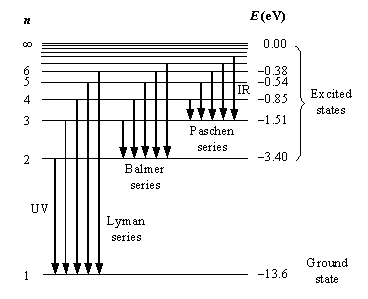
\includegraphics[width=.9\textwidth]{img/01/lyman.jpg} 
        \caption[Raies de l'hydrogène]{Changement de niveau d'énergie de l'atome d'hydrogène}
 		\label{fig:lyman}
\end{figure}

La série de Lyman correspond a la transition atomique menant au fondamental de l'atome d'hydrogène.
Il existe plusieurs série de transition autre que celle de Lyman (cf Fig. \ref{fig:lyman}) mais cette dernière est la plus énergétique et la plus fréquente, et donc la plus facile à détecter.
Il y a émission d'un photon Lyman-alpha pendant la transition de l'électron du premier état excité vers l’état fondamental (n2 -> n1).
L'énergie de cette transition est de 1216 $\AA$,  ce qui place l’émission dans l'Ultra Violet.
Réciproquement, la transition n1 vers n2 mène a l'absorption d'un photon Lyman-alpha.
C'est a dire que si un nuage de gaz neutre se trouve entre une source et l'observateur, le spectre réceptionné présentera une raie d'absorption à 1216 $\AA$.

\subsubsection*{Forêt Lyman alpha}

Maintenant considéreront des distances cosmologique entre la source et l'observateur.
Durant le parcours des photon, l'Univers aura subis une expansion et le spectre d'émission de la source sera redshifté.
Le spectre présentera des raie d’absorption à différents endroit suivant le moment de rencontre des différents nuages de gaz neutre.
C'est série de raies est très dense à haut redshift et est appelée forêt Lyman alpha.

\subsubsection*{Tunnel Gun Peterson}

Si nous considérons maintenant que la source est a l’intérieur d'une zone neutre, la série de raies absorbée ne sera plus discrète mais continue.
C'est ce continuum d’absorption que l'on nomme tunnel Gun-Peterson \cite{1965ApJ...141.1295S}

La figure \ref{fig:spectre_quasar} montre une série d'observations de spectres de quasars.
Ces spectres sont classés par redshift, et le tunnel GP des plus éloigné est particulièrement visible.

%Dans le cas de la reionisation, les sources sont des quasar.
%Les quasars sont des objets suffisamment brillants pour être observé a très grandes distance.
%Il est observé que plus leur redshift est important, plus leur foret lyman alpha est important.
%Les plus lointains d'entre eux présentent  un tunnel gun peterson.

\begin{figure}
        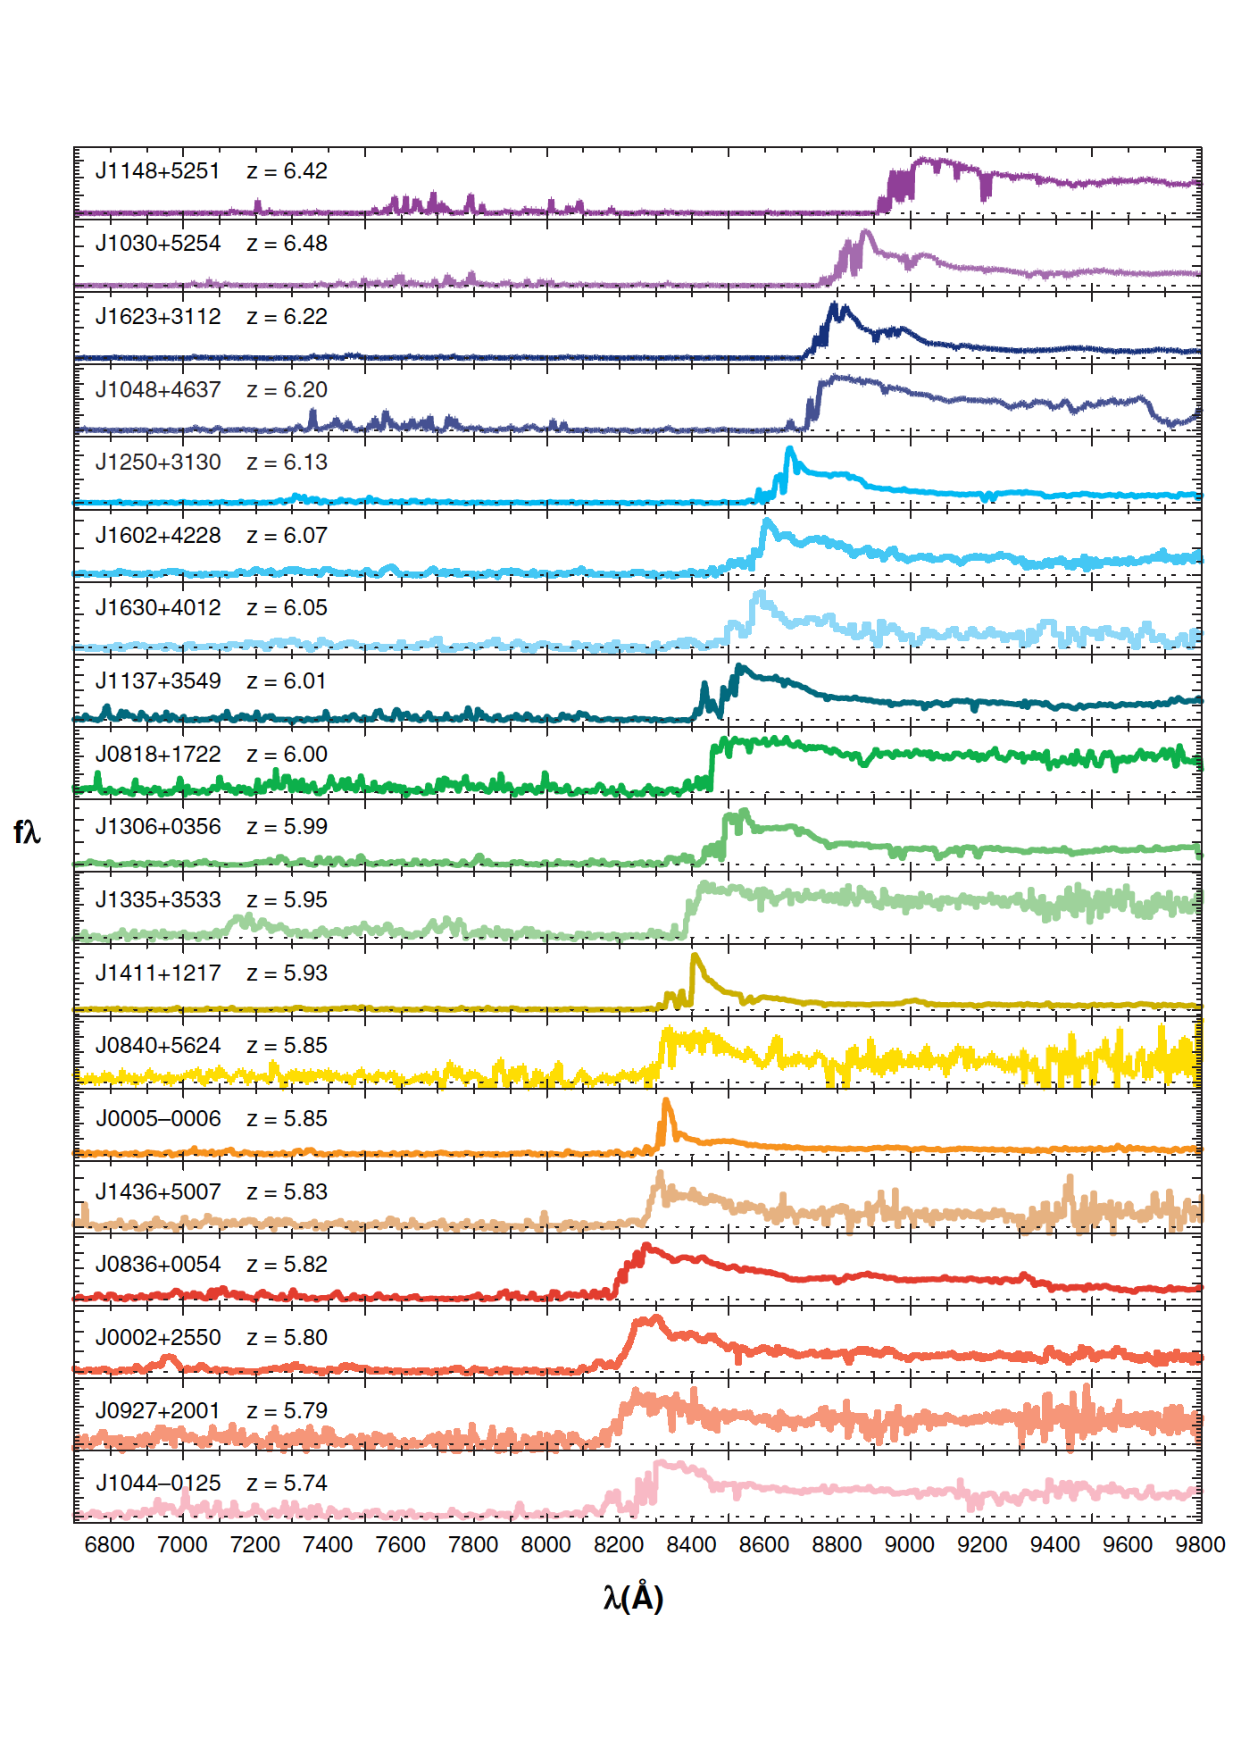
\includegraphics[width=.95\linewidth]{img/01/quasar_spectre.pdf} 
        \caption[Spectre de quasars]{Spectre de quasars à différents redshift présentant un tunnel Gunn Peterson.
		Image extraite de \cite{fan_constraining_2006}.}
 		\label{fig:spectre_quasar}
\end{figure}

\subsubsection{Épaisseur optique}

A partir des spectres obtenu il est possible de mesurer l’épaisseur optique traversée par les photons Lyman alpha à l'aide de la formule suivante:
\begin{equation}
\tau_{GP} = \frac{\pi e^2}{m_e c} f_\alpha \lambda_\alpha H^{-1}(z) n_{HI},
\end{equation}
où $f_\alpha$ est la force d'oscillateur de la transition Lyman alpha, $\lambda_\alpha = 1216 \AA$, $H(z)$ est la constante de Hubble, $n_{HI}$ la densité d'hydrogène neutre.

En appliquant cette formule aux différents spectres observés (figure \ref{fig:spectre_quasar}), \cite{fan_constraining_2006} ont mesurer la variation d'épaisseur optique en fonction du redshift.
Les résultats sont présentés sur la figure \ref{fig:epaisseur_optique_quasar}.
Il apparaît clairement que l'épaisseur optique augmente avec le redshift.

\begin{figure}
        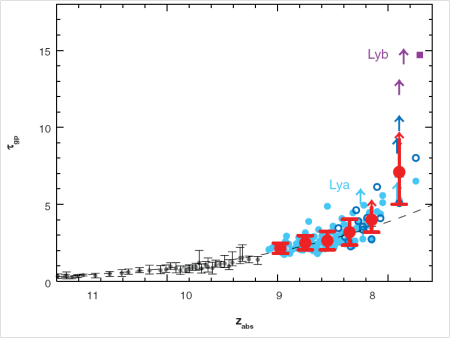
\includegraphics[width=.95\linewidth]{img/01/epaisseur_optique_quasar.png} 
        \caption[Epaisseur optique Lyman alpha]{%https://ism2009.wordpress.com/2009/04/28/on-the-density-of-neutral-hydrogen-in-intergalactic-space/
		Épaisseur optique calculée a partir des spectres de quasar de la Fig\,\ref{fig:spectre_quasar}
        Image extraite de \cite{fan_constraining_2006}.}
 		\label{fig:epaisseur_optique_quasar}
\end{figure}

\subsubsection{Les contraintes sur l'état d'ionisation}

A partir de l'épaisseur optique, il est possible de déterminer la fraction d'hydrogène neutre traversée.
Une compilation des contraintes sur la fraction d'hydrogène neutre a été réalisé par \cite{2015ApJ...811..140B} et est présenté sur la figure \ref{fig:compile_constrains}.
On y observe un brusque changement à redshift $z\approx6$.
Cette chute dans la fraction de neutre représente la fin de la période de réionisation.

\begin{figure}
        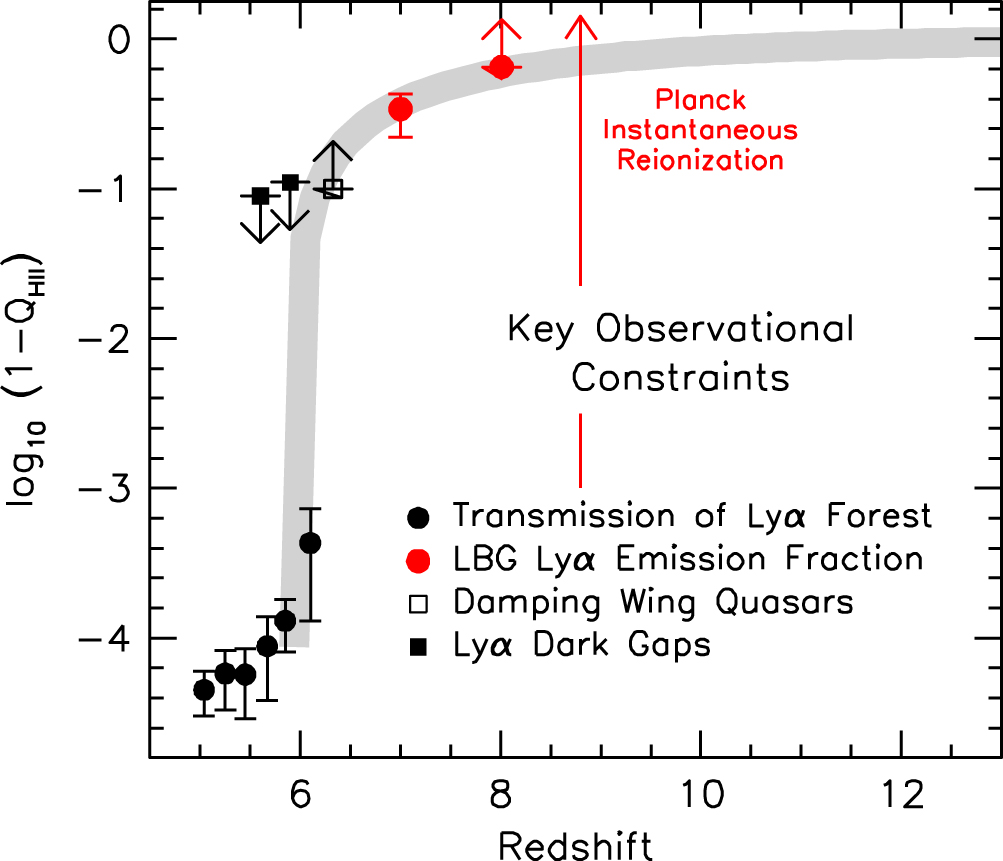
\includegraphics[width=.95\linewidth]{img/01/xionconstrains.jpg} 
        \caption[Fraction de neutre]{Fraction de neutre en fonction du redshift a partir d'observation lymann alpha.
        Compilation par \cite{2015ApJ...811..140B}}
 		\label{fig:compile_constrains}
\end{figure}


\subsection{CMB et épaisseur optique Thomson}

Une observation de la réionisation se trouve également dans les photons CMB, car la réionisation constitue un avant plan qui les a influencé. 
Les photons émis lors de la recombinaisons ont été diffusé, par le grand nombre d'électron libérer pendant la réionisation.
Cette succession de diffusions Thomson, se traduit par une épaisseur optique qui prend la forme : 

\begin{equation}
\tau_z = c \sigma_t \int_z^0 n_e (z) \frac{dt}{dz} dz,
\end{equation}
avec $\sigma_t$ la section efficace Thomson et $n_e (z)$ la densité d'électron libre.

L'épaisseur optique Thomson cesse d'augmenter à partir d'un certain redshift du à l’absence d'électrons libres permettant les diffusions.
Une représentation de cette contrainte, observée par le satellite Planck se trouve sur la figure \ref{fig:epaisseur_optique_thomson}.
Différent modèles réionisation y sont également présentés.
En utilisant un modèle de réionisation instantané, \cite{planck_collaboration_planck_2016} estime le redshift de réionisation à $z_r = 8.8 ^{+1.3}_{-1.2}$.

\begin{figure}
        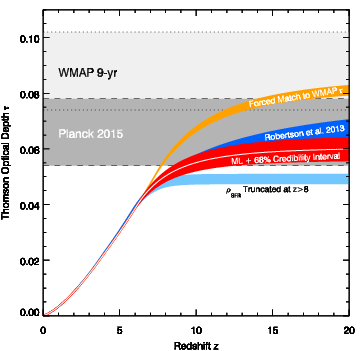
\includegraphics[width=.9\linewidth]{img/01/epaisseur_optique_thomson.png} 
        \caption[Epaisseur optique Thomson]{%https://inspirehep.net/record/1343310/plots
		Contrainte sur l'épaisseur optique Thomson.
        Image extraite de \cite{2015ApJ...802L..19R}
 		\label{fig:epaisseur_optique_thomson} }
\end{figure}

%\subsection{ligne 21 cm}
%
%Une raie a 21 cm est émisse par les nuages d'hydrogène neutre.
%Lorsque que le spin de l'électron et du proton sont opposée, le niveau d'énergie de l'atome est légèrement supérieur au cas ou les spins sont alignés.
%Ces deux niveaux ont des énergies très proches et la transition est dite hyperfine.


%Lors du changement de spin d'un électron 
%
%\subsection{polarisation du CMB)}
%
%\subsection{fonction de luminosité UV}

%\section{Les futures observations}
%\subsection{SKA}
%\subsection{LOFAR}

\section{Quelques questions en suspend}

%quand est ce arrivé?
%quelles sont les sources? -> débat galaxies vs quasars

%En utilisant la halo mass function presenté en TODO REF, 

La provenance des photons qui ont réionisé l'Univers est toujours indéterminée.
En étudiant la répartition du nombre de galaxies en fonction de leurs masses, on observe que les galaxies les moins massives sont nombreuse et que les galaxies les plus massives sont rare.
Or, plus une galaxie est massive, plus celle ci va créer des étoiles, et donc emmètres des photons.
La balance entre les nombreuses galaxies peu lumineuses, et les rare galaxies extrêmement lumineuse reste à déterminer.

De plus, les quasars, objet extrêmement lumineux, situé dans les galaxies les plus massives, augmente encore le budget de photon.
Les quasars ont contribué à réioniser l'Univers mais dans quelles proportion?
Il faut un certain temps pour mettre en place les conditions propices à l'apparition d'un quasar, est ce que ce temps a été suffisant avant z=6, pour en former suffisamment ?
Certain travaux soutiennent que c'est le cas (eg \cite{chardin_large-scale_2017}) cependant seul le rayonnement provenant des galaxies a été considérer lors de cette thèse.

Si ce sont les galaxies qui ont réionisé l'Univers, quelle est le ratio entre la quantité de rayonnement produite et la quantité de rayonnement capable d'atteindre l'\ac{IGM}?
La fraction d'échappement ($f_{esc}$) permet de faire le lien entre les observations et la physique réellement en place au sein des galaxies.
Elles dépend de nombreux paramètres comme la formation stellaire ou les propriétés du milieu.
Comment évolue t-elle en fonction de la masse des galaxies? 

%La figure \ref{fig:gal_AGN} présente le budget de photon plausible pour les galaxies ou les quasars.
%\begin{figure}
%        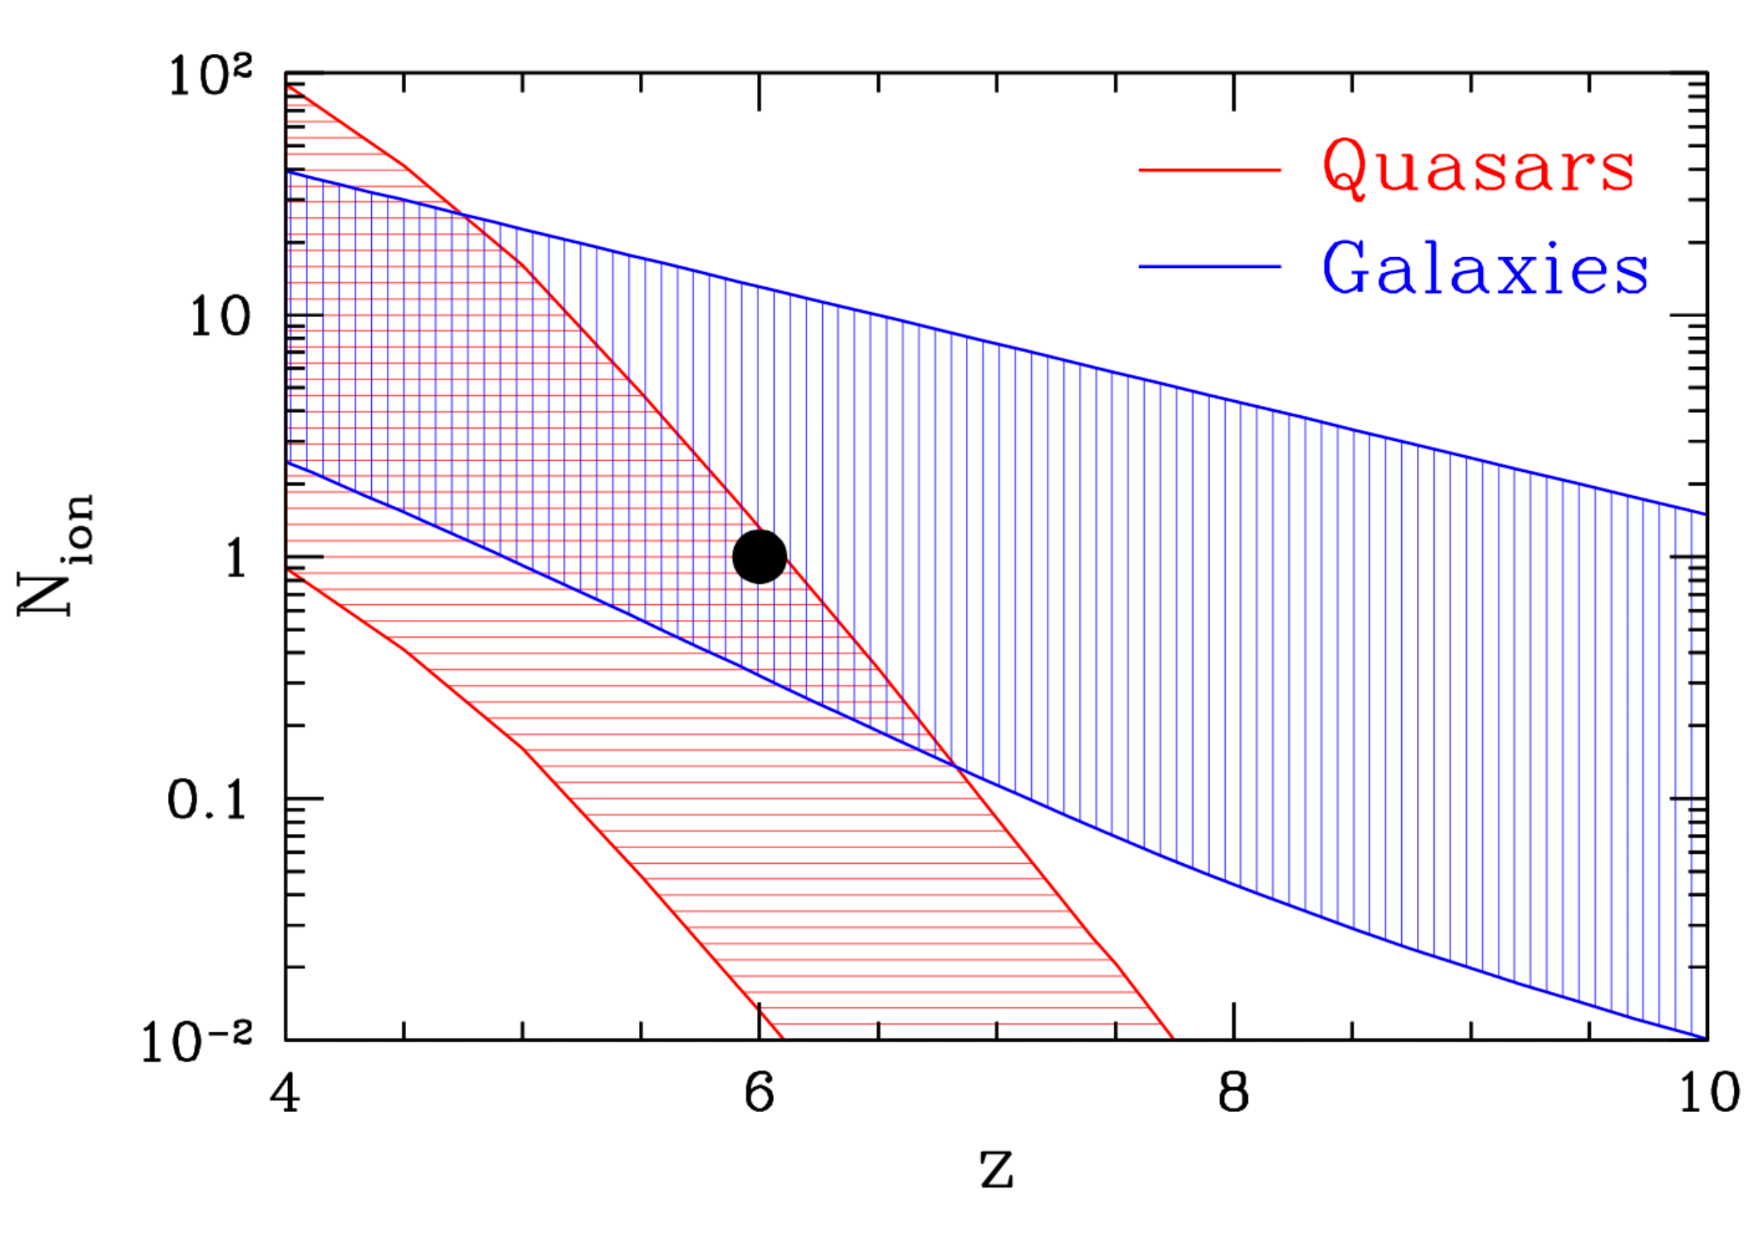
\includegraphics[width=.9\linewidth]{img/01/gal_AGN.pdf} 
%        \caption{Budget de photons provenant des galaxies et des quasars durant la reionization selon \cite{trac_computer_2011}.
% 		\label{fig:gal_AGN} }
%\end{figure}

%outlier dans l'épaisseur optique des quasars
%Le groupe local ?


%%%%%%%%%%%%%%%%%%%%%%%%%%%%%%%%%%%%%%%%%%%%%%%%%%%%%%%%%%%%%%%
%%%%%%%%%%%%%%%%%%%%%%%%%%%%%%%%%%%%%%%%%%%%%%%%%%%%%%%%%%%%%%%

%\ctparttext{\begin{flushright}{\slshape    
%	Premature optimisation is the root of all evil.} \\ \medskip 
%	-- Donald Knuth
%\end{flushright}
%}

%\cleardoublepage
%\ctparttext{Cette partie est liée a la publication présentée en annexe\,\ref{pap:EMMA}.\medskip
%
%\emph{"EMMA: an adaptive mesh refinement cosmological simulation code with radiative transfert"}\medskip
%
%Dominique Aubert, Nicolas Deparis et Pierre Ocvirk
%2015 MNRAS
%}
%\part{Methodes numeriques}
%\chapter{Introduction a EMMA}
\label{ch:introduction}
% (cf loi de \cite{moore1965cramming}). 
%\cite{THOMPSON200620}

%Les échelles de temps sont radicalement opposées entre la cosmologie qui considère les temps les plus long de l'univers et les progrès informatiques qui vont à une vitesse exponentielle.
%Du fait de l'avancée rapide des moyens de calculs, les simulations numérique sont des produits possédant une valeur se dépréciant rapidement et doivent être considérées comme éphémère.

Nous avons vu dans la partie précédente qu'elles étaient les principales physiques à l’œuvre durant l'époque de réionisation.
L'objectif de cette partie est d'expliquer comment ces physiques sont modélisées et quelles sont le contraintes sur leurs implémentations.
On se concentrera particulièrement sur le cas du code EMMA.


%Comment modéliser la reionization?

\section{Aperçu des différents modèles numériques}

Un code de simulation cosmologique a pour vocation principale de suivre l'évolution de différents "fluides", comme la matière noire, la gaz, les étoiles et la radiation (et parfois le champs magnétique).
Ces fluides sont de natures différentes et il n'y a pas de méthode unique permettant de suivre de manière optimale ces différentes physiques.
On distinguera principalement deux catégories de fluides: les collisionnels et les non-collisionnels.

\paragraph{La physique non-collisionnelle} concerne les phénomènes qui n'interagissent pas par collision.
Dans notre cas, il s'agit principalement la matière noire et les étoiles. 

\paragraph{La physique collisionnelle} concerne principalement le gaz.

Il existe conceptuellement deux principales façons de suivre un fluide dans l'espace.
%Ces deux approches sont dites \emph{Eulérienne} ou \emph{Lagrangienne}.
En lien direct avec ces deux familles de représentations physique, il existe deux principales familles de codes cosmologique% : les codes \ac{SPH} et les codes \ac{AMR}.

\paragraph{Représentation Lagrangienne : } 
consiste à se placer au point de vue du fluide.
Une série d'éléments de fluide de masse fixe pouvant se déplacer et/ou se dilater dans l'espace sera considérée.
Les codes utilisant ce type de représentation seront généralement associés avec une gestion de la physique sous forme de \emph{particules}.
Ces codes seront dit \ac{SPH}.

%\paragraph{\ac{SPH} : } représente le gaz sous forme de particule de masse constante mais de taille variable.
%Notion d'arbre -> KDtree

\paragraph{Représentation Eulérienne : } 
consiste à se placer au point de vue de l'espace.
On considère un élément d'espace et le bilan de matière entrant et sortant de chacune de ses interfaces.
On associera généralement les codes utilisant ce type de représentation avec une gestion de la physique sous forme de \emph{grille}.
Si la grille est de résolution variable, on parlera de grille \ac{AMR}.

%\paragraph{Code sur grille} : représente l'espace sous forme de cellules organisées sur une grille. 
%Notion d'arbre -> arbre AMR
%La représentation Lagrangienne la plus populaire (dans le domaine des simulations cosmologiques) est sans doute le \emph{Smouth Particle Hydrodynamics (SPH) }
%Les volumes cosmologiques étant généralement cubique, les éléments de grille le sont généralement aussi.
%historique
%avantage inconvénient AMR vs SPH
%introduction de la grille et de la méthode AMR

Un même code peux utiliser conjointement plusieurs des concepts qui viennent d'être introduits.
Dans le cas présent, EMMA utilise une représentation Lagrangienne pour simuler la physique non collisionnelle de la matière noire et des étoiles, et une représentation Eulérienne pour simuler le gaz et la radiation.

\section{TODO}

avantage inconvénient AMR vs SPH

%TODO
Comparaison a RAMSES


\section{Gestion de la grille}
\label{sec_gestion_grille}
%(nécessaire d'être positionné ici car la structure en arbre conditionne plusieur choix par la suite)

Un des concepts central de EMMA est sa grille adaptative.
Tout les moteurs physiques sont basés dessus et sa structure conditionne un certain nombre de choix par la suite.
C'est pourquoi nous allons la développer ici, avant de détailler la gestion de la physique. 

\subsection{Grille régulière et AMR}
Avant d'aborder le concept de grille adaptative faisons un léger détour par l'exemple d'une grille fixe et régulière.
Dans le cas des simulations sur grille fixe, les données sont réparties en mémoire de façon ordonnée.
Dans un espace en 3D, on accédera à une cellule contenant le point de coordonnées normées $(x,y,z)$ sur une grille de $N_x*N_y*N_z$ cellules, à l'aide de son identifiant Id dans le tableau en mémoire.
\begin{equation}
Id = i + j*N_x + k * N_x*N_y
\end{equation}
avec :
\begin{equation}
\begin{cases}
i=\lfloor x \rfloor \cdot N_x \\
j=\lfloor y \rfloor \cdot N_y \\
k=\lfloor z \rfloor \cdot N_z \\
\end{cases}
\end{equation}
ou $\lfloor a \rfloor$ représente la partie entière de $a$.

Nous voyons ici que l'organisation en mémoire et la recherche de voisin sont relativement simple à gérer.
Les vecteurs sont alloués de manière statique et la recherche de voisin est basée sur un jeu d'indice relativement simple.
Les choses sont plus complexes dans le cas d'une grille adaptative.
Étant amenée à évoluer, il faut introduire des mécanismes permettant de construire ou détruire certaines parties de la grille de façons dynamique.
Ces mécanismes vont totalement changer l'organisation de la grille.

Un exemple de grille \ac{AMR} générée par EMMA est présenté sur la figure \ref{fig:AMR}).
Un fonction de critères prédéfinis par l'utilisateur la résolution de la grille peut être arbitrairement augmentée localement.
L'avantage de ce type de grille est d'économiser des ressources de calcul par rapport au cas d'une grille fixe, ou il faudrait beaucoup plus de cellules pour obtenir une résolution équivalente.

\begin{figure}[bth]
        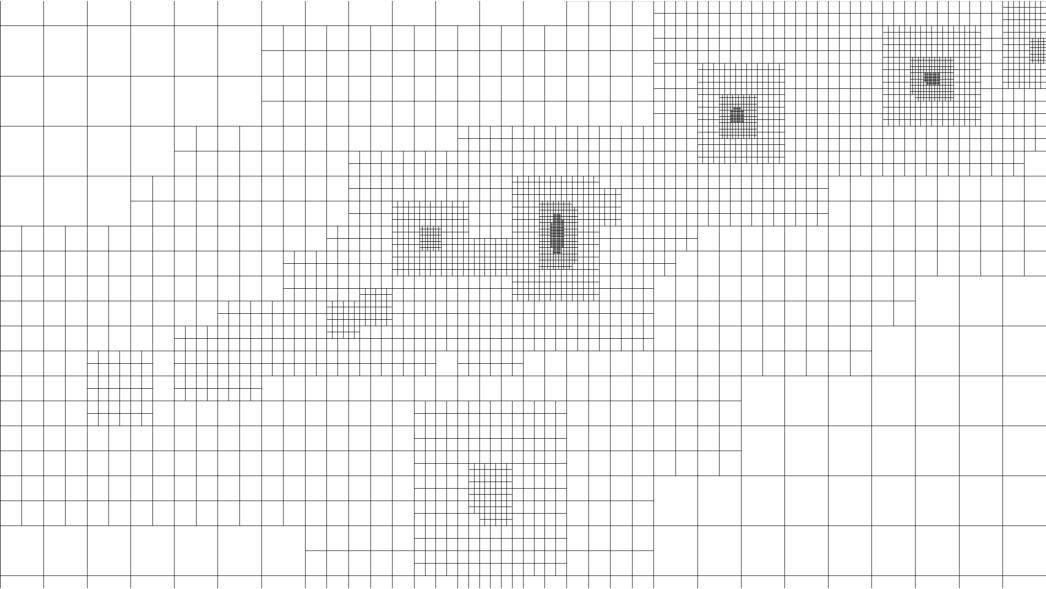
\includegraphics[width=.95\linewidth]{img/02/AMR.pdf} 
        \caption[Grille générée par EMMA]{Exemple de grille \ac{AMR} générée par EMMA. 
        La  résolution de la grille est augmentée arbitrairement dans les régions d'intérêts.
 		\label{fig:AMR}}
\end{figure}

\subsection{Octree}

Il existe deux grands groupe de maille adaptative.
Le premier groupe utilise une séries de grilles fixes imbriquées. %TODO ref
Chaque région raffinée sera une grille fixe de résolution plus importante spatialement liée a une grille de base.
Chaque nouvelle grille aura une résolution double par rapport a la précédente.
Il est possible d'ajouter autant de niveaux que voulu.

Le second est le groupe qu'utilise EMMA : fully threated tree description \citep{khokhlov_fully_1998-1}.
La base de cette représentation est de considérer que chaque cellule est associée à une grille fixe de taille 2x2x2 que l'on nommera un OCT, car décomposé en 8 cellules.
%sous parties qui sont elles même des cellules.
Et récursivement, chacune de ces cellules peuvent à leurs tour être divisée et associée à un OCT.
Il en résultera un arbre nommé Octree, représenté sur la figure \ref{fig:octree}.

\begin{figure}[bth]
        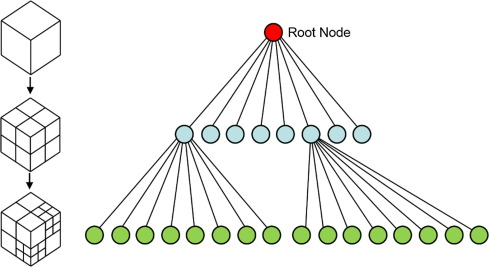
\includegraphics[width=.95\linewidth]{img/02/octree.jpg} 
        \caption[Grille AMR et son octree]{Représentation d'une grille AMR a gauche, et de son octree associé a droite. 
        Image extraite de \cite{SU201659}
     	\label{fig:octree}
}
\end{figure}

%TODO introduire construction de la grille et grille coarse
Pour créer une grille de départ, il faudra d'abord créer un OCT, appelé racine, et le forcer à raffiner.
Chacune de ces nouvelles cellules vont à leurs tours être raffinée.
Cette opération est répétée pour toutes les cellule jusqu'à obtention d'une grille régulière de la taille désirée.
A chaque nouveau raffinement de le nombre de cellule est multiplié par 8.
Le nombre de cellules d'un niveau entièrement raffiné est donc de:
\begin{equation}
N_{cells} = 2^{3L}
\end{equation}
où $L$ est le niveau de raffinement.

Il en résultera une grille régulière qui ne pourra pas être dé-raffinée par la suite.
Le niveau de cette grille de base sera appelé niveau \textit{coarse}.

\subsubsection{La structure OCT}
%et liste chainée

Il existe une bimodalité entre la représentation de la grille en mémoire et la représentation de l'espace physique.
Comme la grille est amenée à évoluer, il n'y a plus une position unique en mémoire associée à une position dans l'espace.
De plus, le nombre d'éléments de la grille change au cours du temps.
Il faut donc conserver à la fois l'information de la position dans l'espace physique et dans l'espace mémoire.

En principe, on allouera une certaine quantité d'OCT en mémoire qui constituerons une réserve.
On viendra ensuite piocher dans cette réserve pour ajouter des éléments à la grille.
Les OCT de la grille seront organisés sous forme de liste chainées, il est donc nécessaire d'avoir l'information de la position de l'OCT précédent et de l'OCT suivant en mémoire.

Pour créer un lien entre elle, il est nécessaire de stocker l'information de voisinage.
L'information spatiale est aussi contenue dans les OCT, ceux ci disposent de six pointeurs vers les cellules voisine.
Un OCT est également composé d'un tableau de huit cellules filles, ainsi que d'un pointeur vers sa cellule mère.
Un OCT qui n'a pas de cellule mère est appelé OCT racine, en pratique il n'y en a qu'un seul, de niveau 0, et il représente l'ensemble de l'espace de la grille..
La génération de conditions périodique (généralement utilisées en cosmologies) se fait de manière naturelle en faisant pointer tout les voisins de l'OCT racine vers lui même.
La structure minimal d'un OCT de EMMA est présenté sur le listing \ref{lst:oct}.

\begin{lstlisting}[float=bth,language=C,frame=tb,caption={La structure OCT de EMMA},label=lst:oct]
struct OCT{
  struct CELL cell[8]; // les 8 cellules de l'oct
  struct CELL *nei[6]; // pointeurs sur les cellule voisines
  struct CELL *parent; // cellule mere
  struct OCT *next;    // oct suivant dans la liste chainee
  struct OCT *prev;    // oct precedent dans la liste chainee
  int level;           // niveau de l'oct
};
\end{lstlisting}

\subsubsection{La structure CELL}
\label{sec:CELL}
Les cellules contiennent l'information physique (densité, pression, température, etc...).
Chaque cellule peut, sous certaine condition, être subdivisée en un OCT pour augmenter la résolution localement.
L'information de la position de la cellule dans l'OCT parent est contenue dans son identifiant (allant de 0 à 7).
Une CELL qui n'a pas d'OCT enfant est dite cellule feuille.
La structure minimal d'une CELL de EMMA est présenté sur le listing \ref{lst:cell}.

\begin{lstlisting}[float=bth,language=C,frame=tb,caption={La structure CELL de EMMA},label=lst:cell]
struct CELL{
  int id;            // permet de determiner la position de la cellule dans l'oct
  struct OCT *parent // l'oct pere de la cellule
  struct OCT *child; // si child est different de NULL alors la cellule est raffinee et child point vers l'oct enfant
  struct PHYSIC *data; // pointeur vers la partie physique
  struct PARTICLE *part; // pointeur vers la chaine de particules.
};
\end{lstlisting}


\subsubsection{La structure PARTICULE}
\label{sec:PART}

%TODO introduire liste chainée de particule

Nous verrons dans la section \ref{sec:solverDM} qu'une partie de la physique est résolue sous forme de particule.
Il est donc nécessaire d'ajouter un champs de particule à la grille \ac{AMR}
Comme les OCT, les particules utilisent une représentation sous forme de liste chaînée, et chaque cellule dispose de sa propre liste chaînée de particules.
Lors de raffinement cette liste devra être découpée et distribuée entre les nouvelles cellules crées.
Une particule est essentiellement caractérisée par sa position, sa masse et sa vitesse.
On ajoutera a ceci son statut, qui sera utilisé pour différentier les particules de matière noire des particules stellaires. 
Le listing \ref{lst:part} présente la structure minimale d'une particule dans EMMA.


\begin{lstlisting}[float=bth,language=C,frame=tb,caption={La structure PARTICULE de EMMA},label=lst:part]
struct PART{
  REAL3 x;  // vecteur position
  REAL3 v;  // vecteur vitesse
  struct PARTICULE *next;  // particule suivante
  struct PARTICULE *prev;  // particule precedente
  int idx;  // identifiant unique
  int  isStar;  // matiere noire ou etat de l'etoile
  REAL t;       // instant de creation
  REAL mass;    // masse
};
\end{lstlisting}



%TODO introduire la structure part

\subsection{Gestion du raffinement}
\label{sec:raffinement}
%différentes condition de raffinement.\\
%sur la matière noire\\
%semi Lagrangienne\\
%sur le gradient d'ionization\\
%sur le gradient de densité (shock)\\
\subsubsection{Condition de raffinement}
Il est possible de définir arbitrairement une condition de raffinement en fonction de la physique que l'on cherche a étudier.
Par exemple, dans des tests unitaires de type sphère de Stömgren (cf \ref{sec:stromgren}) ou explosion de Sedov (cf \ref{sec:sedov}), on marquera les cellules qui sont soumises à un gradient d'ionisation ou de densité supérieur à un certain seuil pour suivre l'évolution du front.
Dans le cas de simulations cosmologique, on utilisera généralement une condition en densité dite semi-Lagrangienne.
C'est a dire qu'une cellule sera marquée comme "à raffinée" si la masse de matière noire (ou de gaz) qu'elle contient est supérieur a huit fois la masse de matière noire (ou de gaz) moyenne d'une cellule de ce niveau.
%le deraffinement
On remarquera que la condition de raffinement ne prends pas en compte le fait qu'une cellule soit déjà raffinée ou non.
Si une cellule est raffinée, mais qu'elle n'est pas marquée comme "à raffinée" elle sera donc dé-raffinée.

\subsubsection{En pratique}
Le raffinement se fera en trois temps:

\begin{itemize}
\item Dans un premier temps le code va passer en revue toutes les cellules d'un niveau, et les marquer comme "à raffiner" si une première condition physique est respectée.

\item Une fois tout le niveau passé en revue, le code va ensuite faire une série de $N_{buffer}$ passages sur tout le niveau en marquant à chaque fois toues les cellules voisine des cellules précédemment marquées.
Cette zone de $N_{buffer}$ cellules autour des zones soumises à la condition physique de raffinement sera appelée le "buffer de raffinement".
Ce tampon a pour but d’élargir la zone de raffinement et ainsi permettre une transition douce entre les niveaux.
De plus il ne sera autorisé à n'avoir qu'un seul niveau de décallage au maximum lors des transitions.

\item Une fois les cellules respectant ces deux conditions marquées, le raffinement est effectué.
\end{itemize}

%En pratique le raffinement d'une cellule se fera en lui associant un OCT.
%*child pointera alors vers le dernier OCT libre de la liste chaînée.


\subsubsection{Opérateurs de changement de grilles} 
\label{Opérateurs de changement de grilles}

Les opérations de raffinement/dé-raffinement font intervenir des opérateurs de changement de grille.
Le changement de résolution peut avoir lieu dans les deux sens :

\begin{itemize}
\item La \emph{restriction} consiste à dégrader la grille en résolution. 
La restriction la plus directe consiste à moyenner les cellules à dégrader. 
Par exemple, sur une grille à deux dimensions, pour diviser la résolution par deux, quatre cellules de la grille de départ devront être moyennées pour obtenir une nouvelle cellule de la grille à base résolution.

\item La \emph{prolongation} consiste à augmenter la résolution d'une grille, la prolongation la plus directe consiste à injecter les valeurs de l'ancienne grille dans un certain nombre de cellules de la nouvelle grille. (fig \ref{Opérateurs de changement de grille})
\end{itemize}

\begin{figure}
\begin{center}
\subfloat[Restriction]{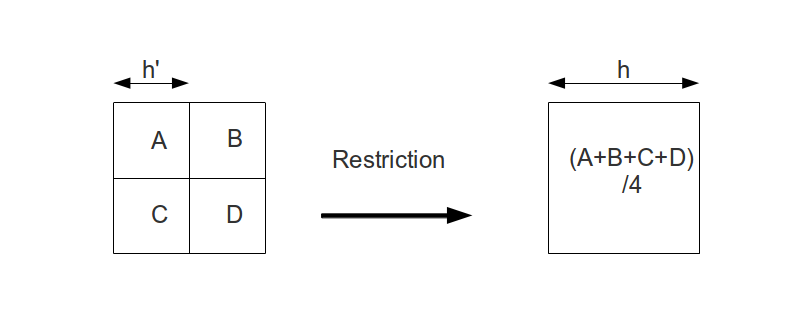
\includegraphics[width=.45\linewidth]{img/02/Restriction.png}}
\subfloat[Prolongation]{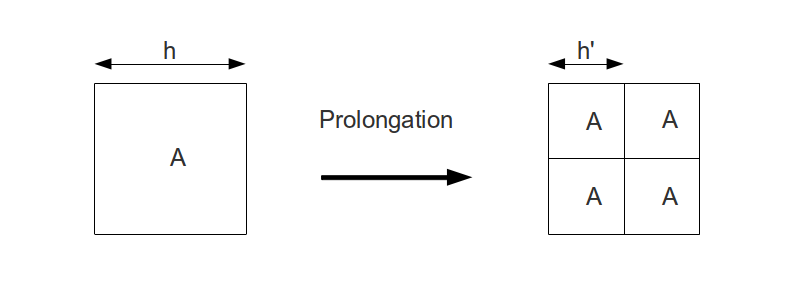
\includegraphics[width=.45\linewidth]{img/02/Prolongation.png}}\\
\subfloat[Niveau L  ]{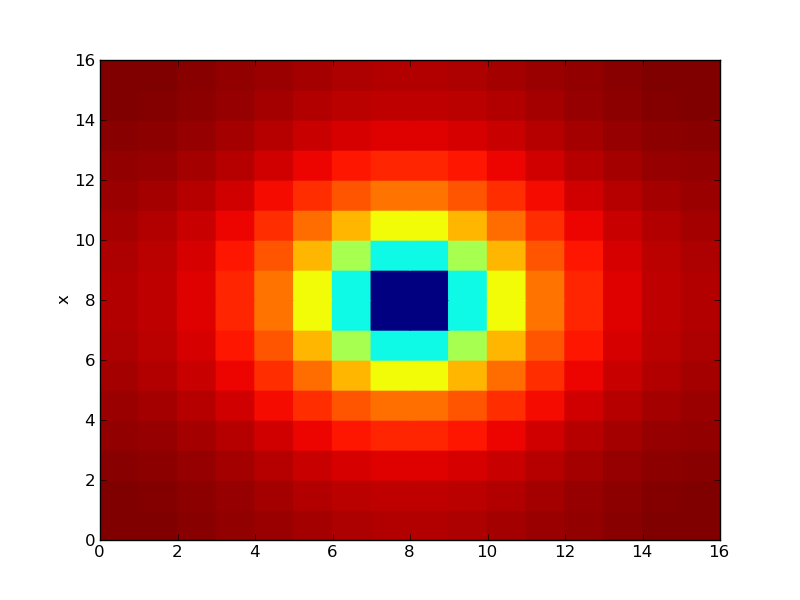
\includegraphics[width=.45\linewidth]{img/02/0090.png} \label{Opérateurs de changement de grille d}}
\subfloat[Niveau L+1]{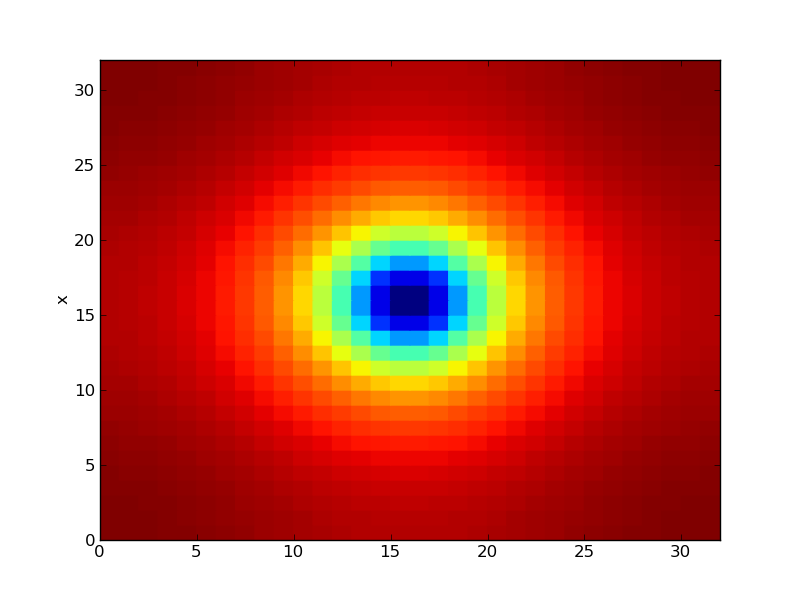
\includegraphics[width=.45\linewidth]{img/02/0088.png} \label{Opérateurs de changement de grille c}}
\caption[Opérateurs de changement de grille]{Opérateurs de changement de grille. 
Ils permettent de changer la résolution de la grille. 
Un exemple de restriction consiste à moyenner une valeur de plusieurs cellules, la prolongation associée consiste en une injection directe d'une valeur dans plusieurs cellules.
\label{Opérateurs de changement de grille}}
\end{center}
\end{figure}

%La prolongation et la restriction sont des opérateurs aisément parallélisables. Chaque cellule (ou paquet de huit cellules) est indépendante des autres et il est possible de ne changer la résolution que d'une partie de la grille sans en affecter le reste.

%Il existe principalement deux conditions sur les opérateurs de changement de grille. 
%La première impose une certaine réciprocité entre eux, les opérateurs doivent être adjoints: il est nécessaire qu'après une prolongation, suivie d'une restriction la grille d'arrivée soit la même que la grille de départ. 
%L'inverse n'est pas nécessairement vrai: après une restriction, de l'information est perdue et aucune prolongation ne pourra la recomposer.
%La seconde condition concerne la precision des opérateurs, il est nécessaire que la somme des ordres des opérations soit supérieure à l'ordre de l'équation à résoudre. 
%Ici, la restriction est d'ordre trois, la prolongation d'ordre un et le Laplacien d'ordre deux, cette condition est vérifiée.

\subsection{Gestion du pas de temps}

Sur une grille \ac{AMR}, le pas de temps n'est pas uniforme.
Du fait de la condition de Courant, un niveau raffinée aura un pas de temps plus court que le niveau de base.
Comme dans notre cas, une cellule est raffinée en divisant par 2 chacune de ces dimensions, le pas de temps sera lui aussi divisé par 2.
Il faudra donc réaliser 2 évolutions d'un pas de temps raffiné pour être synchronisé avec un niveau inférieur, et ce de manière récursive.
L'évolution entre les niveaux se fera en suivant le schéma présenté sur la figure \ref{fig:timestep}.

\begin{figure}
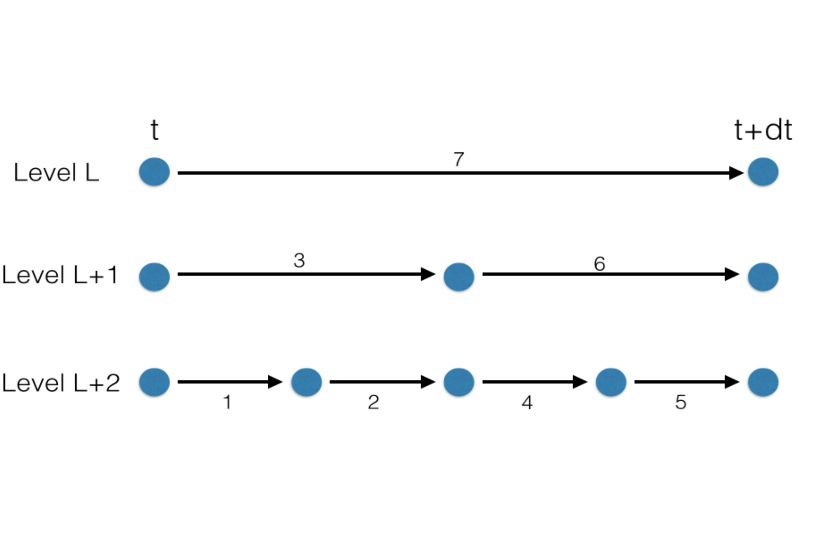
\includegraphics[width=.95\linewidth]{img/02/tstep.png}
\caption[Pas de temps AMR]{Gestion du pas de temps en fonction des niveaux raffinées.
Un niveau évolue par pas de temps deux fois plus court que celui de son niveau supérieur.
\label{fig:timestep}}
\end{figure}


\subsection{Gestion de l'expansion}
\label{sec:supercomobil}

%On parlera de simulations cosmologiques lorsque l'e volume considéré est en expansion.

Nous avons vu dans l'introduction à la physique de la reionisation que l'énergie noire représente la majore partie du contenu de l'univers (cf \ref{sec:dark_egy}) .
Nous allons voir dans cette partie comme cette composante est traitée numériquement.
Bien que nous ne sachions absolument pas ce que peux être physiquement l'énergie noire, nous en observons les effets : l'Univers est en expansion accélérée.
Le moteur gérant l'énergie noire n'est pas a proprement parler un moteur numérique, mais plutôt d'un système d'unité. % servant a normaliser la physique.
Il consiste a normaliser les grandeurs par une variable fonction du facteur d'expansion.

L'intégration de la cosmologie, régissant le lien en le temps et le facteur d'expansion sera réalisé une fois au moment de l'initialisation du code (cf Eq. \ref{eq:scale_t}).
Il en résultera une table, conservée en mémoire pendant toute l'exécution.
Le facteur d'expansion sera alors interpoler dans cette table en fonction de l'avancement de la simulation.% (cf partie calcul du pas de temps) %TODO ref

Il existe deux possibilités pour modéliser l'expansion de l'univers à l'aide d'une grille.
La première consiste a considérer un élément de volume $dx$ de taille fixe, et au fur et a mesure que l'univers grandis, à y ajouter des éléments.
Le problème et que le coût numérique de la simulation croit, entre autre, avec le nombre d'éléments que l'on considère.
La seconde possibilité est de faire varier la taille des éléments de calcul avec le facteur d'expansion.
On appellera les longueurs ainsi exprimées des longueurs comobile.

\begin{equation}
r=a r'
\end{equation}

ou $r$ représente une longueur en unités physique et $r'$ en unités comobile.
Ainsi un cube de 10 Mpc physique de coté, pris aujourd'hui, aura une taille de 10 Mpc comobile (cMpc) aujourd'hui, mais aussi a redshift z=9 ou sa taille physique ne sera plus que de de 1Mpc physique.
De plus, il est généralement pratique de normaliser les grandeurs que l'on considère. 

\begin{equation}
r'=\tilde{r}r*
\end{equation}
ou $\tilde{r}$ est la longueur normalisée et $r*$ le facteur de normalisation.

La généralisation de ce principe a d'autre unités que la longueur est appeler système d'unités supercomobiles \citep{martel_convenient_1998}.

\begin{table}
\begin{center}
\begin{tabular}{r l} \hline 
Longueur: & $\tilde{r}=\frac{r}{ar_*}$ \\ \hline 
Densité de matière: & $\tilde{\rho}=\frac{\rho a^3}{\rho_*}$ \\ \hline 
Vitesse: & $ \tilde{v}=\frac{av}{v_*}$ \\ \hline 
Pas de temps: & $\tilde{dt}=\frac{dt}{a^2t_*}$\\ \hline 
Densité d’énergie potentielle: & $\tilde{\Phi}=\frac{a^2 \Phi}{\Phi_*}$\\ \hline 
Pression: & $\tilde{p}=\frac{a^5 p}{p_*}$\\ \hline 
Densité d’énergie cinétique: & $\tilde{\epsilon}=\frac{a^2 \epsilon}{\epsilon_*}$\\ \hline 
Densité D’éléments: & $\tilde{N}=a^3 N r_*^3$\\ \hline 
Flux: & $\tilde{F}=a^4 r_*^2 t_* F$\\ \hline 
\end{tabular} 
\end{center}
\caption[Système d'unité supercomobile]{Passage du système d'unités physique vers le système d'unité supercomobile} 
\end{table}

\begin{table}
\begin{center}
\begin{tabular}{r l} \hline 
Longueur  & $r_*=L$\\ \hline 
Densité & $\rho_* = \bar{\rho} = \frac{3H_0^2 \Omega_m}{8\pi G}$\\ \hline 
Temps & $t_* = \frac{2}{H_0 \sqrt{\Omega_m}}$\\ \hline 
Vitesse & $v_* = \frac{r_*}{t_*}$\\ \hline 
Potentiel & $\Phi_* = \frac{r_*^2}{t_*^2} = v_*^2$\\ \hline 
Pression & $p_* = \frac{\rho_* r_*^2}{t_*^2} = \rho_* v_*^2$\\ \hline 
Énergie & $\epsilon_* = \frac{p_*}{\rho_*} = v_*^2$\\ \hline 
\end{tabular} 
\end{center}
\caption[Facteurs de normalisation]{Facteurs de normalisation des différents grandeurs physique} 
\end{table}

\subsubsection{Gestion du pas de temps}
L'évolution de la grille sera limité d'un pas de temps à l'autre.
La condition condition pour effectuer le calcul du pas de temps sera:
\begin{equation}
\frac{\delta a (\Delta t) } {a} < \epsilon
\end{equation}

\subsection{Recherche de voisin}
\label{sec:voisins}
Nous verrons par la suite que l'état d'une cellule dépend des états des cellules qui l'entoure.
La recherche de voisins est une étape importante dans la gestion de la grille et se fera en suivant les étapes présenté sur la figure \ref{fig:voisin}.
Dans le cas ou la voisine se trouve dans le même OCT la recherche est immédiate.
Mais dans le cas ou la voisine n'est pas dans le même OCT, il faut trouver l'OCT voisin, vérifier que celui ci est géré par le même processus et vérifier si il est raffiné.
Cette recherche peut être complexe et couteuse, on prendra donc garde à minimiser les appels de la fonction de recherche. 

\begin{figure}[bth]
        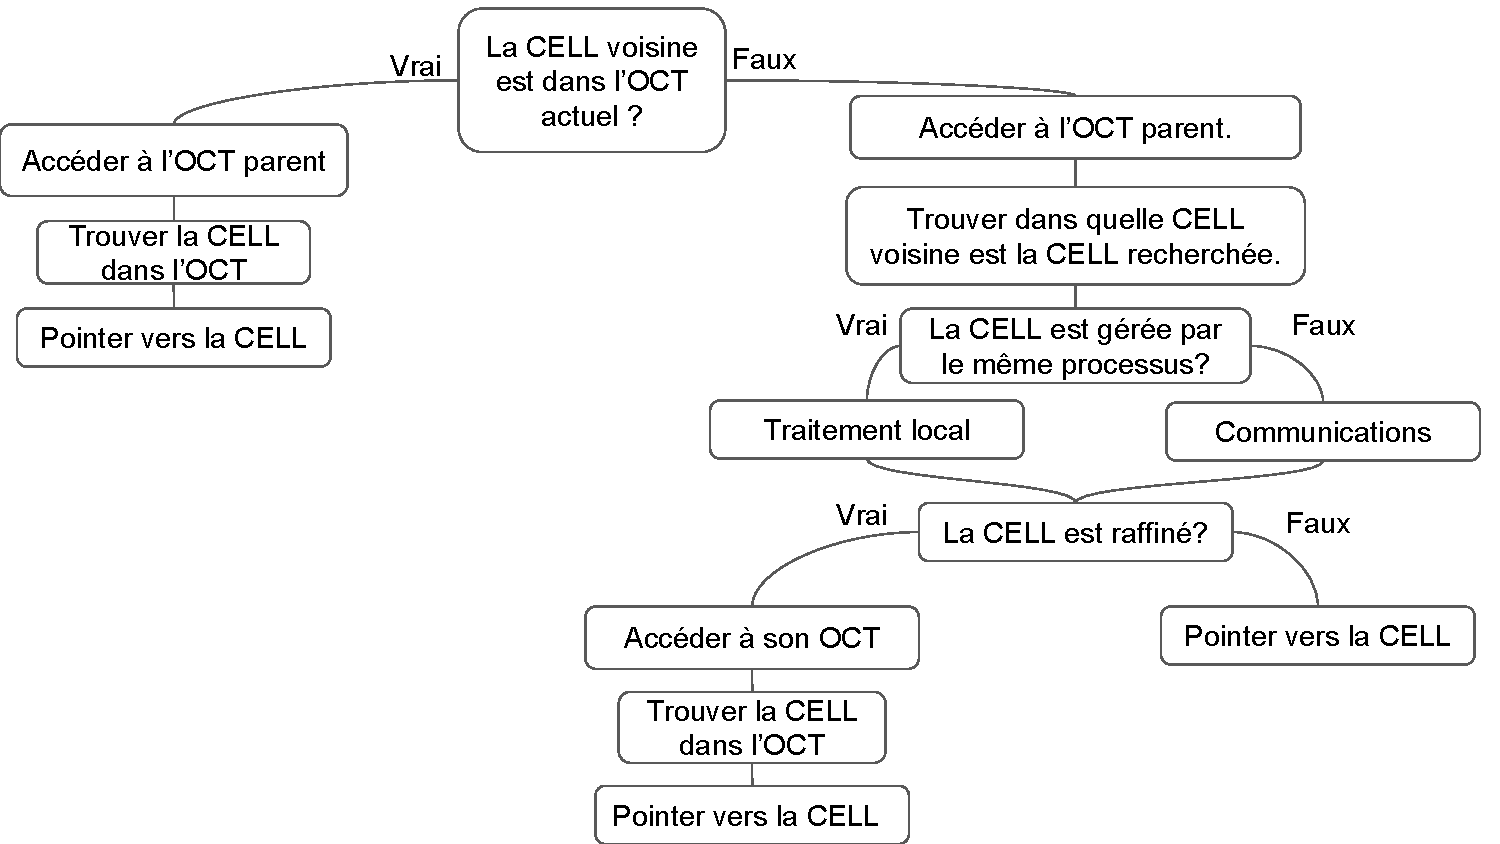
\includegraphics[width=.95\linewidth]{img/02/voisins.pdf} 
        \caption[Recherche de voisin dans l'octree.]{Arbre décisionnel pour la recherche de voisin dans l'octree.
        La recherche de voisins n'est pas triviale et peu avoir un coût non négligeable.
     	\label{fig:voisin} }
\end{figure}

%\begin{itemize}
%\item en fonction de l'ID de la cellule courante, déterminer si la voisine recherchée est dans le même OCT parent.
%
%\item
%\begin{itemize}
%\item Si c'est le cas: accéder à l'OCT parent, et à l'aide de l'indice du tableau de cellule, retrouver le voisin en question.
%\item Si ce n'est pas le cas, accéder à l'OCT parent, à l'aide des pointeurs sur les voisins, localiser l'OCT voisin et s'y rendre. Si l'OCT est raffiné déterminer 
%\end{itemize}
%
%\end{itemize}
%\include{Chapters/part_02/solver}
%
\chapter{Matériel et parallélisme}
\label{sec:materiel}
%Nous avons a ce stade un aperçu du type de calcul a effectuer, essayons d'estimer . 
%De plus, les simulations cosmologiques ont pour principal défi de simuler d'important volume d'espace avec la meilleure résolution possible.

Le défis des simulations de la réionisation est qu'elles doivent simuler un volume d'Univers suffisant grand pour être représentatives de la variance cosmique et converger sur la taille des régions HII ($\approx 100$ Mpc selon \cite{iliev_cosmological_2006}) tout en résolvant la formation stellaire (échelle $<1$ pc).
En première approximation, il nous faudrait donc échantillonner un tel volume par $\left( \frac{100Mpc}{1pc} = 10^7 \right) ^3 = 10^{21}$ éléments.
Ce qui est totalement impossible à l'heure actuelle.
%Nous verrons dans la prochaine partie que nous sommes encore loin de pouvoir résoudre la formation stellaire dans ce type de simulations. %TODO ref
Nous avons vu que l'amélioration de certains algorithmes (passage de grilles fixes à grilles adaptatives, intégration du potentiel plutôt que somation N-corps directe, etc... voir chapitre \ref{ch:introduction}) a permis d'augmenter significativement la taille des simulations à puissance de calcul identique, mais le principal facteur limitant reste au niveau du matériel.

\section{Calcul hautes performances}

Le calcul hautes performance ou \ac{HPC} est un domaine visant à utiliser au mieux les ressources de calculs disponibles.
Ces ressources peuvent être multiples et les utiliser conjointement de manière efficace représente un challenge en soit.
Dans cette partie nous allons aborder une série de concepts liés au \ac{HPC}, utiles à la compréhension des simulations cosmologiques.


\subsection{Loi de Moore et simulations}
La loi de Moore \citep{moore1965cramming} propose un doublement du nombre de transistor par circuit intégré tout les 18 mois environs. (Fig \ref{fig:moore})
Comme la puissance de calcul est étroitement liée à cette évolution, la taille -- le nombre d'éléments de résolution -- des simulations, suit également cette croissance exponentielle (Fig. \ref{fig:taillesimu}).

\begin{figure}
        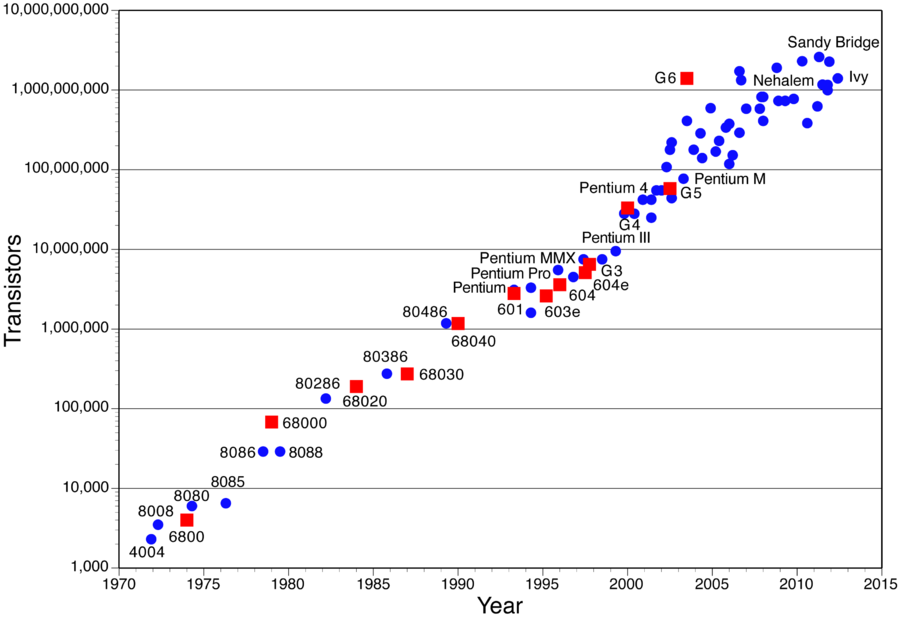
\includegraphics[width=.95\linewidth]{img/02/moorelaw.png} 
        \caption[Loi de Moore]{Nombre de transistor par processeur en fonction du temps ou loi de Moore}
 		\label{fig:moore}
\end{figure}

\begin{figure}
        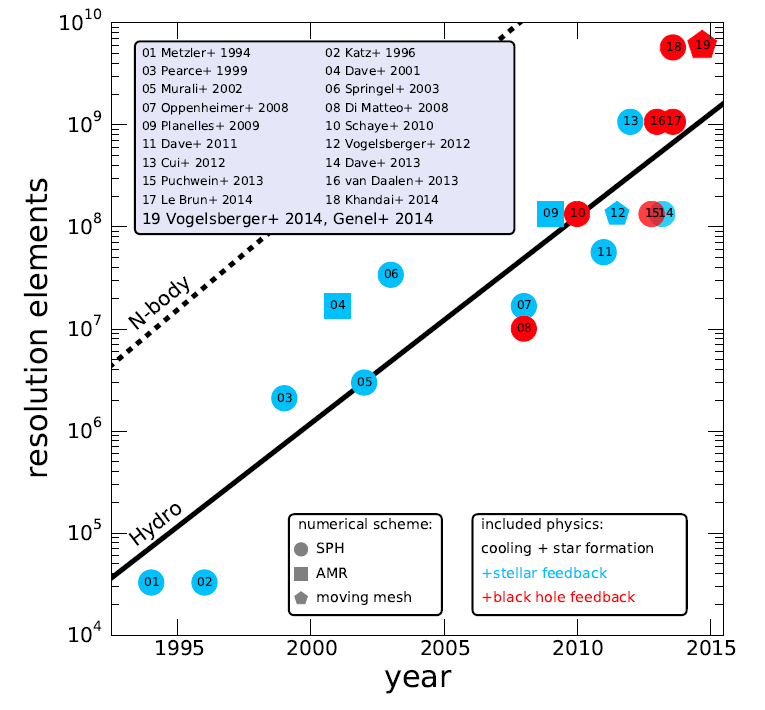
\includegraphics[width=.95\linewidth]{img/02/figure_simulations_with_time.png} 
        \caption[Évolution de la taille des simulations]{Évolution de la taille des simulations en fonction du temps.
        Il existe un lien direct avec la loi de Moore.
        Image illustris}
 		\label{fig:taillesimu}
\end{figure}


\subsection{Principes de parallélisation}

A cause de limitations physiques comme la taille des atomes ou la capacité de refroidissement du silicium, on ne peut pas créer des processeurs arbitrairement denses en transistors et aussi puissants que ce que l'on souhaite.
La technique utilisée pour continuer à augmenter la puissance de calcul consiste à en utiliser plusieurs en même temps.
Dans le cas des simulations cosmologiques, la parallélisation est effectuée en découpant l'espace à simuler en un certain nombre de sous-domaines chacun associé à une unité de calcul.
Comme chaque sous-domaine n'est pas isolé, mais appartient au même ensemble, les domaines vont devoir communiquer entre eux sur l'état de leurs voisins.
Nous verrons en détails comment est effectué ce découpage dans la section \ref{sec:parasoft}.
Mais voyons d'abord un aperçu des contraintes techniques de la parallélisation.

Il existe différents types de parallélisations définis par la taxonomie de Flynn \citep{Flynn:1972:COE:1952456.1952459}: 

\begin{itemize}
\item SISD Single Instructions on Single Data.
Aucun parallélisme, exécution d'une unique série d'instructions sur un unique flux de données.

\item SIMD Single Instructions on Multiple Data.
Exécution d'une unique série d'instructions sur différents flux de données.
C'est le principe de fonctionnement des GPU.

\item MISD Multiple Instructions on Single Data 
Exécution de différentes série d'instructions sur un seul flux de données.

\item MIMD Multiple Instructions on Multiple Data.
Exécution de différentes série d'instructions sur différents flux de données.
C'est l’architecture la plus utilisée aujourd'hui, et celle qui nous intéresse ici.
Le type MIMD est lui même découpé en deux sous ensembles : 

\begin{itemize}
\item On dit que la mémoire est \textit{distribuée} quand les processus ont leurs propres espaces mémoires dédiés.
Les principales machines que j'ai pu rencontrer utilise un modèle MIMD à mémoire distribuée.

\item On dit que la mémoire est \textit{partagée} quand plusieurs processus ont accès au mème espace mémoire.
Ce type de gestion mémoire est généralement associée à des systèmes plus petits que le modèle de mémoire distribuée.
\end{itemize}
\end{itemize}


\subsection{Les calculateurs}
\label{sec:titan}

Il existe plusieurs niveaux de parallélisation, au niveau matériel.
Par exemple, un processeur actuel dispose de plusieurs cœurs, capable de gérer chacun un processus (parfois plusieurs dans le cas de l'hyperthreading).
Il est possible d'avoir plusieurs processeurs au sein d'un même ordinateur.
Et il est possible d'utiliser conjointement plusieurs ordinateurs.
Ce qui nous mène à la notion de centre de calcul.

La production de simulations cosmologiques à haute valeur scientifique se fait sur des centres de calcul.
%A la manière d'un télescope pour les observateurs, les supercalculateur sont les outils principaux des simulateurs.
%Et a la manière des plus gros télescopes, ces calculateurs sont gigantesques.
La figure \ref{fig:titan} présente le calculateur TITAN du Oak Ridge Leadership Computing Facility sur lequel ont été exécutées les simulations CoDa \citep{ocvirk_cosmic_2015} et CoDa I AMR (voir section \ref{sec:CODAEMMA}).
En novembre 2015, TITAN a été classé deuxième plus puissant calculateur au monde selon le cite top500.org (cf \ref{tab:top500}), il est aujourd'hui quatrième.

\begin{figure}
        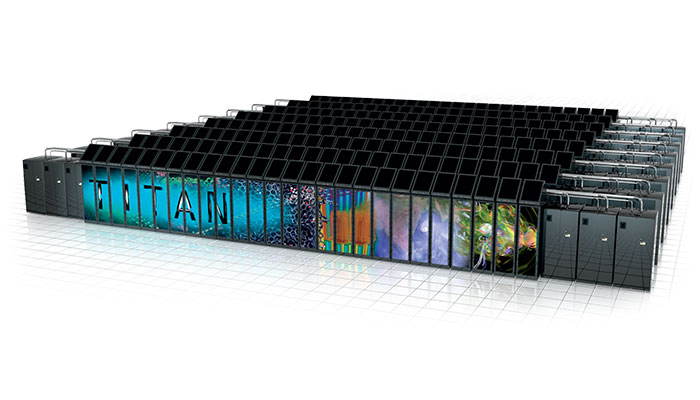
\includegraphics[width=.95\linewidth]{img/02/titan.jpg} 
        \caption[Titan]{Supercalculateur Titan OLCF.
        La calculateur sur lequel ont été exécutés les simulations CODA}
 		\label{fig:titan}
\end{figure}

\begin{table}
\begin{tabular}{ l l l l }
\hline 
Système & Pays & nb de cœurs & TFlop/s (peak) \\
\hline 
Sunway TaihuLight & Chine & 10,649,600 & 125,435.9 \\ 
Tianhe-2  & Chine & 3,120,000 & 54,902.4 \\ 
Piz Daint  & Suisse & 361,760 & 25,326.3 \\ 
Titan  & États unis & 560,640 & 27,112.5 \\ 
Sequoia  & États Unis &1,572,864 & 20,132.7 \\ 
\end{tabular} 
\caption[TOP500]{Les 5 super calculateurs les plus puissants du top500 de Juin 2017, source : www.top500.org}
\label{tab:top500}
\end{table}

Ce type de calculateur est composé d'un certain nombre de nœuds qui communiquent entre eux par l'intermédiaire d'un réseau.
Un nœud est un élément conceptuellement proche d'un ordinateur personnel puisqu'il dispose d'une carte mère, avec un (ou plusieurs) processeur ou \ac{CPU}, de la mémoire RAM, un SSD/HDD et parfois un \ac{GPU}.
D'une manière générale, plus des composants sont physiquement éloignés, plus leurs communications seront lentes (cf \ref{tab:debits}).
La quantité d'informations passant par une interface représente un certain coût et on cherchera à minimiser ce coût en optimisant le transfert des données à différents niveaux.

\begin{table}
\begin{tabular}{ l l }
\hline 
Interface  & Débit théorique \\
\hline 
Cache L1 & $\approx$ 700Go/s \\
RAM & $\approx$ 20 Go/s \\ 
PCIE 16x & $\approx$ 16 Go/s \\
InfiniBand & $\approx$ 5 Go/s \\
SSD & $\approx$ 600 Mo/s \\
HDD & $\approx$ 100 Mo/s
\end{tabular} 
\caption[Débits interfaces HPC]{Ordre de grandeur des débits théorique des différentes interface rencontrées lors de l'exécution d'un code \ac{HPC}.
On cherchera à optimiser les communications utilisant les interfaces les plus lentes.}
\label{tab:debits}
\end{table}

%Les cœurs au sein d'un même CPU pourront communiquer entre eux de faible quantité de données par l’intermédiaire du cache, ou en passant par la RAM pour les volumes plus importants.

%Proche d'un ordinateur personnel un nœud est composé d'une carte mère sur laquelle est relié entre autres, un ou plusieurs processeurs (CPU), une certaine quantité de mémoire RAM et parfois une carte graphique (GPU)
%Chaque CPU dispose d'un certain nombre de cœurs, et chaque cœurs est capable d'exécuter un certain nombre de processus ou thread (généralement 1, parfois 2 dans le cas de l'Hyperthreading)

%Une fois les processus et les domaines identifiés il existe différentes facons de faire dialoguer les processus entre eux.
%La principale distinction viendra généralement de si les threads sont exécutés par un meme noeud ou non.
%
%, cad par exemple que si le thread 0 déclare une variable X, le thread 1 aura aussi accès a cette variable . 
%OpenMP est une API permettant ce  genre partage de mémoire.

%Si les threads sont exécutés sur un même nœud on aura tendance a utiliser un schéma a base de mémoire partagée.
%
%Dans le cas ou les threads sont exécutés par des processeurs étant physiquement éloigné, ie sur des noeuds différents, les communications doivent passer par un réseau de communication reliant les noeuds.
%Il faudra utiliser dans ce cas une autre API pour explicitement envoyer et recevoir des paquets d'information
%L'API la plus communément utilisée pour ce genre de communication est Message Passing Interface MPI.
%
%\paragraph{Nœud :} Élément du centre de calcul relier par un réseau.
%
%La difficulté est de géré la façon dont les threads travaillent ensemble.
%En effet a chaque thread sera associé un domaine de calcul représentant une partie de l'espace a modéliser.
%De plus les domaine ne sont pas isolés et partage de l'information. 
%
%Nous sommes alors confronté a plusieurs problèmes: comment associer les threads aux domaines de calculs  et comment faire communiquer ces threads entre eux.
%
%Ces machines se composent d'un certain nombre de nœuds.

Généralement, la mémoire est partagée au sein d'un nœud et distribuée sur le réseau.
C'est-à-dire que tous les processus au sein d'un même nœud pourront communiquer par l'intermédiaire de la RAM, ce type de communications est donc rapides.
Pour les communications entre les nœuds, l'information devra passer par le réseau et ce type de communications est donc plus lent.
Et ce d'autant plus que les nœuds sont physiquement éloignés entre eux.

\section{Implémentation du parallélisme}


\subsection{Courbe de Peano-Hilbert}
\label{sec:parasoft}

%https://books.google.fr/books?id=sbQqBgAAQBAJ&pg=PA26&lpg=PA26&dq=peano+hilbert+mpi&source=bl&ots=HgSw0Jpf7d&sig=vXTb2JkDixd1gcDGANoARIYHAG0&hl=fr&sa=X&ved=0ahUKEwilofzKoerSAhUF6RQKHXzQDC4Q6AEIGjAA#v=onepage&q=peano%20hilbert%20mpi&f=false

Dans EMMA la distribution des domaines utilisés pour la parallélisation est réalisée à l'aide d'une courbe de remplissante d'espace.
%Durant le développement d'un code HPC, on cherchera a minimiser les communications
%, et plus spécifiquement celle par le réseau qui sont nombreuse et relativement lentes.
%Warren et Salmon
Dans le but de garder une certaine proximité spatiale, le découpage des domaines de calcul correspondants aux différents processeurs, utilise une courbe de Peano-Hilbert.
Ce type de courbes fractale a la particularité de remplir l'espace en passant par tout les points d'une grille, et donc d'obtenir une représentation 1D d'un espace 3D.
Ainsi si l'on applique ce pavage aux cellules de notre grille, en associant un indice reliant une cellule à sa position sur la courbe de Hilbert, il suffit ensuite de découper la courbe en parties identiques pour définir quelles cellules seront associées à quels processus.
Si l'on a par exemple 32 cellules à assigner sur 4 processeurs, la courbes sera découpée en 4 parties de 8 cellules.
Chacune de ces parties sera en suite assignée à un processeur.
Ce type de découpage minimise les interfaces entre domaines, en s'assurant d'une certaine proximité spatiale entre tout les points de la courbe.

\begin{figure}
        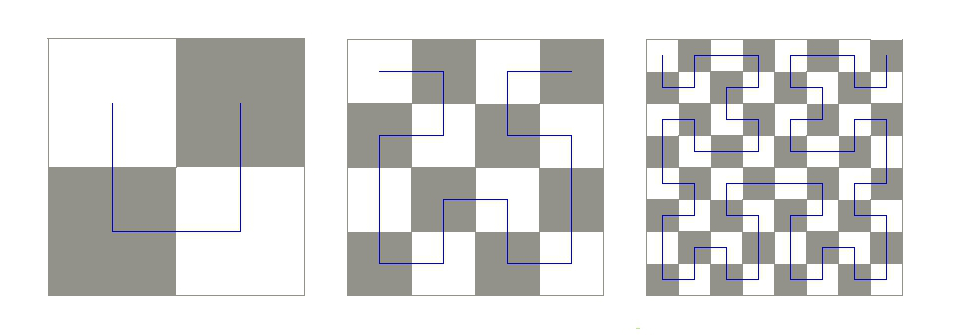
\includegraphics[width=.95\linewidth]{img/02/courbe_Hilbert.jpeg} 
        \caption[Courbe de Hilbert]{Principe de la courbe de Hilbert.
        Ce type de courbe est utilisée pour gérer le découpage des domaines utilisés pour la parallélisation.
        %http://www.lifl.fr/~pmathieu/transform/fractales.html
 		\label{fig:hilbert}}
\end{figure}

%
%\begin{figure}[bth]
%        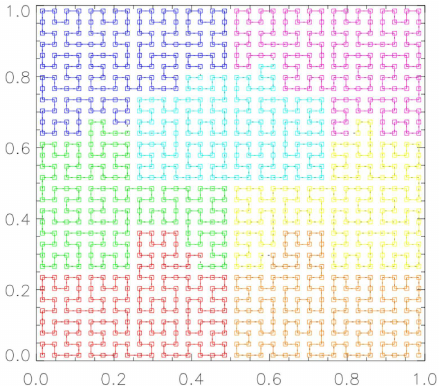
\includegraphics[width=.95\linewidth]{img/02/hilbert2.png} 
%        \caption{exemple de courbe de Hilbert. 
%%http://iopscience.iop.org/article/10.1086/590370/pdf 
%}
% 		\label{fig:hilbert2}
%\end{figure}

Dans l'état actuel de EMMA, la courbe est calculée au début de la simulation, et seule la grille de base est prise en compte.
La répartition des domaines est statique et n'évolue pas au cours de la simulation.
Dans le cas où un domaine raffine plus qu'un autre, la charge de travail y est plus importante.
Dans le futur, l'objectif serait de calculer la courbe de Hilbert sur la totalité des cellules feuilles, pour ainsi pouvoir refaire le découpage et équilibrer la charge entre les processeurs.
%, et réaliser un équilibrage de charge.


\subsection{Les domaines}

Chaque processus dispose d'un domaine de calcul correspondant à une sous partie de la grille.
Cependant, les domaines doivent communiquer entre eux et doivent être sensible a la structure \ac{AMR} de leurs voisins.
Pour répondre à ce problème, EMMA utilise le "Local essential tree decomposition" \citep{Warren:1993:PHO:169627.169640}.
Chaque processus dispose d'une vue globale de toute la grille ( cf Fig. \ref{fig:domaine}) mais la partie de la grille qui n'appartient pas au processeur est vue a résolution dégradée.
Ceci facilite grandement le gestion des conditions de bords.

\begin{figure}
        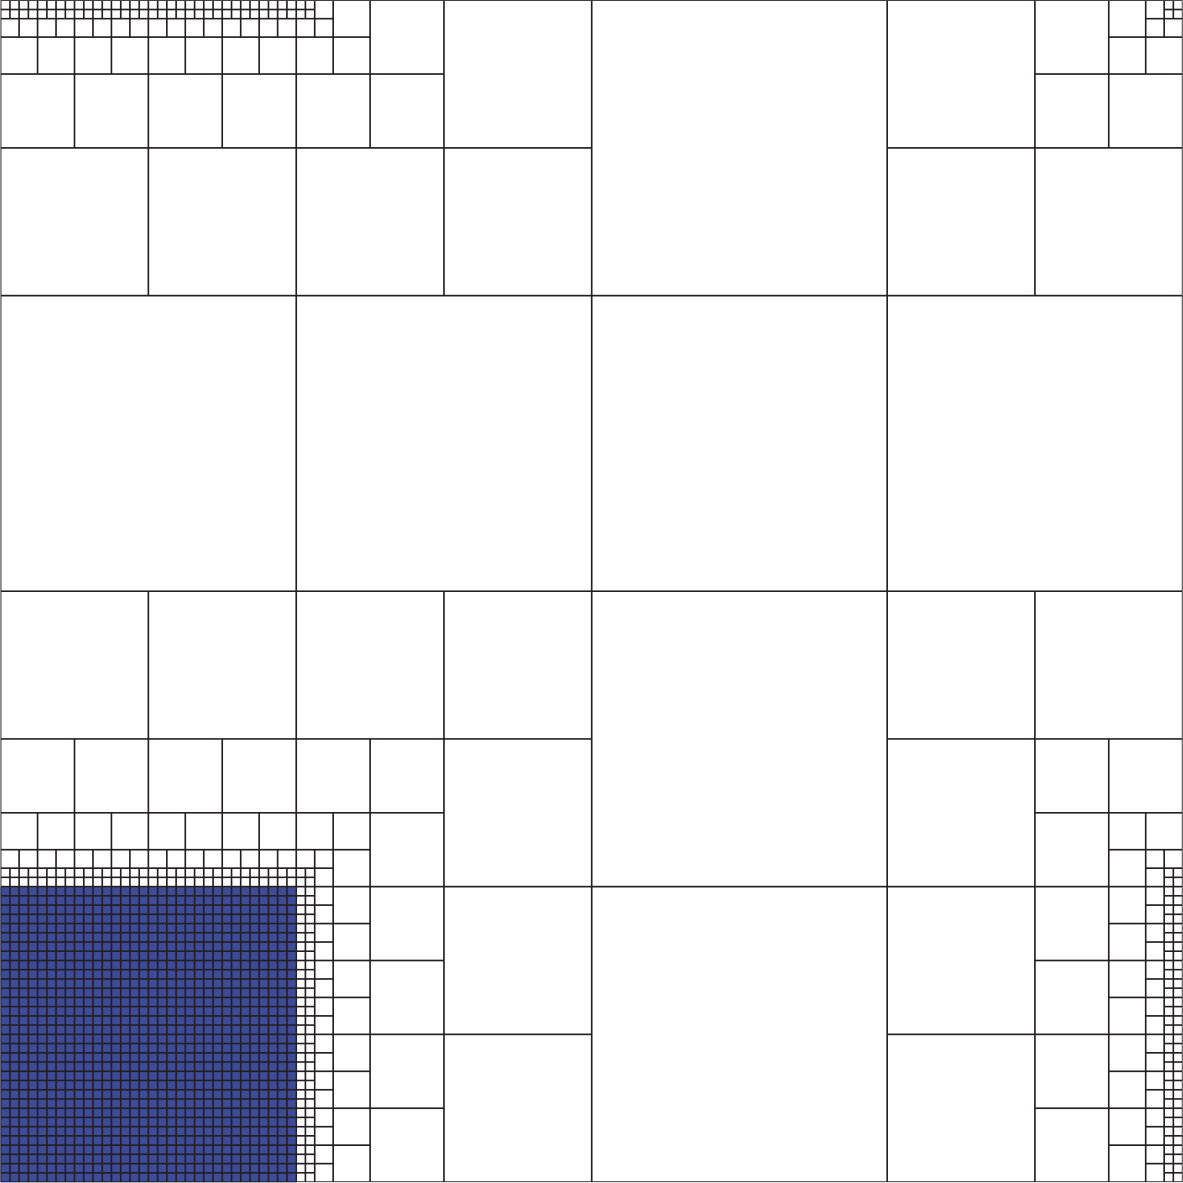
\includegraphics[width=.95\linewidth]{img/02/secteur.png} 
        \caption[Domaine associé à un processus]{Exemple de domaine de processeur généré par EMMA. 
        Chaque domaine représente une vue d'ensemble de la grille, à résolution dégradée.
}
 		\label{fig:domaine}
\end{figure}



\section{Calcul accéléré par processeurs graphiques}
\label{sec:gpu}

EMMA utilise un degré supplémentaire de parallélisation.
Les calculs de chaque domaines sont accélérés en utilisant les capacités parallèles des processeurs graphiques récents.
Les cartes graphiques, ou \ac{GPU} ont été détournées de leur utilisation principale d'affichage il y a une dizaine d'années et offre une capacité de parallélisation importante. 

À l'inverse des \ac{CPU} actuels qui disposent d'un nombre réduit de cœurs, les \ac{GPU} disposent d'une nombre beaucoup plus important de cœurs.
Par exemple un AMD Opteron 6300 de TITAN dispose de 16 cœurs, contre 2880 cœurs pour une NVIDIA Tesla k40c.
Un \ac{CPU} peut exécuter des taches différentes sur chacun de ses cœurs (MIMD) tandis ce que les \ac{GPU} utilisent un mode de parallélisation de type SIMD (Fig \ref{fig:cpugpu}).
Ce mode de parallélisation en font des unités de calculs efficaces dans l'application d'un traitement identique sur un grand nombre d'informations en parallèle.
Elle sont donc toutes indiquées dans le cas des simulations numériques où l'objectif est justement d'appliquer un traitement identique à un grand nombre de cellules.

\begin{figure}
        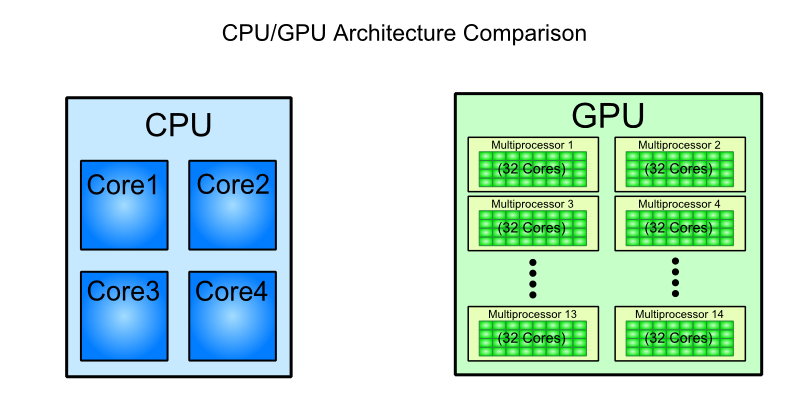
\includegraphics[width=.95\linewidth]{img/02/cpu_vs_gpu.png} 
        \caption[Comparaison CPU/GPU]{Comparaison CPU/GPU. Un \ac{CPU} dispose d'un nombre réduit de cœurs capables d’exécuter des opération complexe. 
        A l'inverse un \ac{GPU} dispose d'un grand nombre de cœurs pouvant exécuter un grand nombre d'opérations simples en parallèle}
 		\label{fig:cpugpu}
\end{figure} 

De plus, il existe au niveau matériel, deux avantages des \ac{GPU} par rapport aux \ac{CPU}.
\begin{itemize}
\item Premièrement leurs meilleurs ratio puissance de calcul sur coup (flop/€).
\item Et également un meilleur ratio puissance de calcul sur puissance électrique (flop/W) ce qui réduit les besoins de refroidissement et permet des économies supplémentaires.
\end{itemize}

% utilise une approche proche du concept de mémoire distribuée, c'est à dire que leurs espaces mémoire ne sont pas commun.


%On tirera le maximum des capacités d'accélération d'un \ac{GPU} avec un code qui est hautement parallélisable.

%Il faut donc que la quantité de calcul effectués par la carte soit suffisante pour rentabilisé la communication.
%plus dur a programmer, performance dépends du problème.


%Or a l'heure actuelle cette communication utilise une interface relativement lente (PCI express) qui rend coûteuse la communication. 

% et de 12Go de mémoire et a une puissance de calcul de 4.3 Tflop/s en simple precision.
%
%
%Intel® Xeon® X7560 -> TDP 130 W -> 76 Gflop/s (crete)
%
%
%IBM A2 (sequoia) -> 204 Gflop/s -> TDP 55W


\subsection{Les communications CPU/GPU}
\label{sec:cpugpu}

\ac{CPU} et \ac{GPU} sont indissociables est doivent être utilisé conjointement pour tirer le meilleurs parti des capacités de calcul offertes par une machine hybride.
Une code hybride est découpé en deux parties, une partie séquentielle exécutée sur le \ac{CPU} et une partie parallèle exécutée sur le \ac{GPU}.
La programmation sur carte graphique impose de gérer les différents espaces mémoire le passage de \ac{CPU} à \ac{GPU} va nécessiter des communications.

Les \ac{CPU} sont capable d'accéder rapidement aux informations en mémoire, quel que soient leurs organisations.
Le \ac{GPU} sont quant à eux sensibles à la segmentation des données.
C'est à dire que les calculs sur \ac{GPU} seront plus performants si les données sont organisées de façons à ce que leurs accès mémoire consécutifs soient physiquement proches.
%Prenons l'exemple d'une différence finie. 
%Pour calculer le nouvel état d'une cellule, il est nécessaire de connaitre sont état actuel, et celui de sa voisine.
%L'accès mémoire sera plus rapide si l'information est situer sur un espace mémoire adjacent.
%Ce choix est motivé par le fait qu'une structure mémoire bien organisée peux amener a des gains conséquents.
Par exemple dans CUDATON \citep{aubert_radiative_2008} un code de transfert radiatif sur grille fixe, le gain de la parallélisation \ac{GPU} est de l'ordre de $80$ car la structure mémoire est optimisée.

La difficulté est que l'arbre \ac{AMR} ne respecte pas cette organisation, et la mémoire peut être extrêmement fragmentée à cause de la liste chaînée (voir section \ref{sec:listechainee}).
Pour limiter l'impact de la fragmentation, le choix a été fait d'organiser les données sur le CPU, avant de les envoyer dans l'espace mémoire du \ac{GPU}.
Cette opération sera appelée "gather" (cf Fig. \ref{fig:gatherscatter}).
Les données organisées sont envoyés sur le \ac{GPU}, pour effectuer les calculs.
Le résultat est ensuite copié sur le \ac{CPU} et remises dans l'arbre par le \ac{CPU} (opération de "scatter").
Dans le cas où les calculs sont réalisés sur le \ac{CPU}, cette opération est quand même réalisée, dans le but de conserver une certaine cohérence entre les versions.

\begin{figure}
        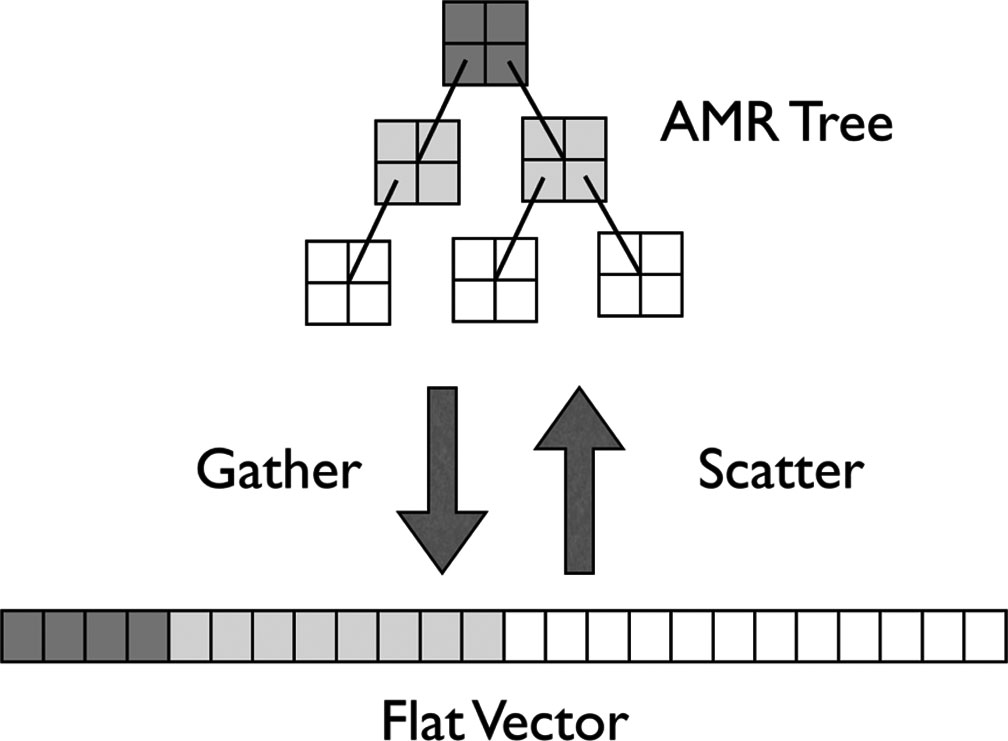
\includegraphics[width=.95\linewidth]{img/02/gatherscatter.jpg} 
        \caption[Passage AMR / vecteur]{Transition entre la structure en arbre de l'AMR et la structure en vecteur de calcul.
        L'arbre est sur le CPU, le vecteur est sur le GPU.
 		\label{fig:gatherscatter}
 		}
\end{figure}

Le pari est ici que la perte de temps générée par les opérations de gather/scatter sera compensé par l'accélération du \ac{GPU} .

En pratique l'opération de gather consiste à rassembler toutes les informations nécessaire au calcul de l'état d'une cellule.
Par exemple pour le calcul du potentiel (cf sec. \ref{sec:solverDM}) les données nécessaires seront: la densité locale, le potentiel local, le potentiel des 6 cellules voisines suivant les axes principaux.
Ces données sont rassemblées dans une structure, puis une série de structures est stockée dans un tableau.
Cette opération sera réalisée par paquet de $N$ cellules pour chaque cellule de la grille.

On peut observer ici que les copies ont beaucoup de redondance.
La copie est composée d'une cellule centrale et des 6 cellules voisines, le ratio information utile sur information nécessaire est de $1/6$.
En passant à la cellule suivante, la cellule précédente sera de nouveau copiée et au final le potentiel d'une cellule sera donc copié sept fois sur le \ac{GPU}.
Ces multiples copies diminuent grandement les performances et en font l'une des principales limitations à l'accélération globale du code.
Toute fois, même dans cet état, l'exécution s'en trouve accélérée d'un facteur $\approx 3$ par rapport à la version \ac{CPU}.
En pratique, l'exécution sur \ac{GPU} permet de significativement réduire la part du calcul dans le cout globale de la simulation.
La principale limitation ne provenant plus de la quantité de calculs mais des opérations tierces comme le gather, le scatter (voir figure \ref{fig:fracgatherscatter}).


\begin{figure}
        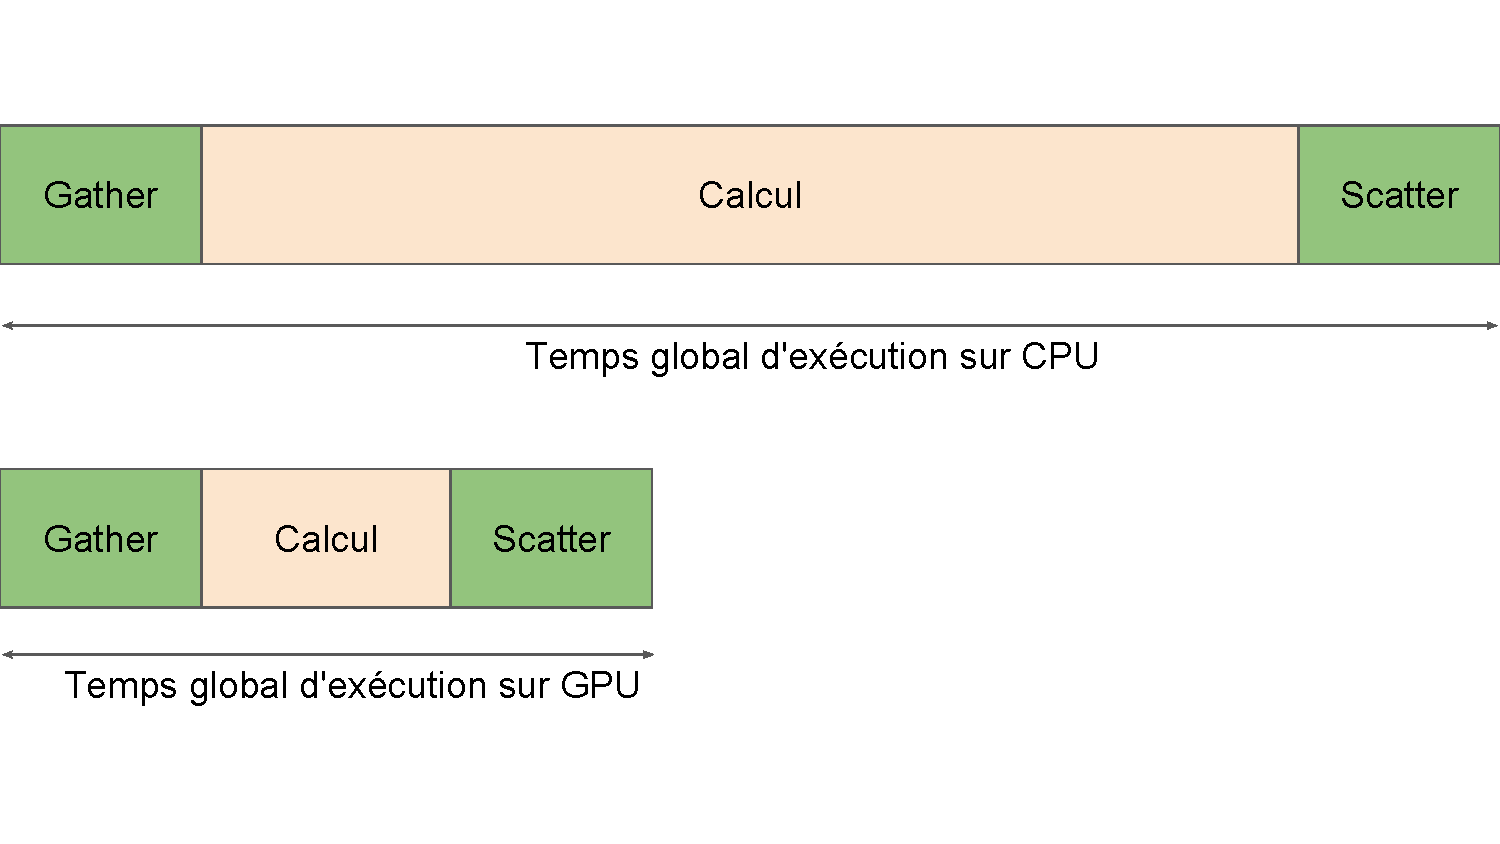
\includegraphics[width=.95\linewidth]{img/02/gsCPUGPU.pdf} 
        \caption[Comparatif coût CPU et GPU]{Comparatif des coûts relatif des opération de gather et scatter en fonction de l'exécution sur CPU ou GPU.
        L'exécution sur GPU permet de réduire fortement le cout du calcul, cependant le coût des opérations tierces est peu impacté, ces dernière deviennent alors les principales limitations de l'accélération globale.
 		\label{fig:fracgatherscatter}
 		}
\end{figure}


Dans le but de réduire le nombre de copies et d'accélérer l'exécution du code, j'ai modifié les opérations de gather/scatter pour diminuer la redondance des copies.
Au lieu de traiter les cellules unes par unes, l'idée est de traiter les octs.
Dans ce cas les cellules sont alors traitées par 8 et les voisinages au sein d'un oct n'ont pas besoin d'être copiés plusieurs fois.
On copie donc 8 cellules d'intérêt et 4 cellules de bord par face du cube, soit 24 cellules.
Le ratio utile/nécessaire passe donc à $8/24 = 1/3$.
La quantité de copies redondantes a donc été divisée par 2 par rapport au cas précédent.

Vu que la surface d'un cube augmente avec le carré de son coté, alors que son volume augmente avec son cube, plus grand sera la nombre de cellules d'intérêts, meilleur sera le ratio.
En étendant ce principe, j'ai développé une méthode qui permet de manière récursive d'envoyer une portion d'\ac{AMR} contenue dans un OCT de niveau arbitraire.
Cependant les résultats ne sont pas à la hauteur des espérances, et l'accélération n'est pas proportionnelle au ratio de données utiles.

Il existe cependant des pistes pour améliorer ce goulot d'étranglement.
Une possibilité est de séparer la gestion de l'arbre de la physique.
En l'état actuel, les données physiques sont stockées en mémoire avec la même structure que l'arbre.
L'idée serait de stocker dans l'arbre, des indices de cellules permettant de retrouver l'information physique dans des vecteurs plats (cf Fig. \ref{fig:gatherscatter}).
Ainsi les vecteurs pourraient être en permanence sur le \ac{GPU}, et seule l'information sur leurs positions dans l'\ac{AMR} devrait être transmise.
Un grand nombre de copies seraient alors évitées. 

Une autre possibilité serait de placer l'intégralité de l'arbre sur le \ac{GPU}.
Dans ce cas, toutes les copies seraient supprimées mais c'est le \ac{GPU} qui devra gérer l'évolution de l'arbre. 
%Il existe des techniques optimisé de gestion d'arbre sur \ac{GPU} à base de "Z-order curves"

\subsection{Courbe de Morton}

Une des évolutions en cours de EMMA, est l'utilisation de courbe de Morton ou Z-order curve \citep{morton1966computer} pour géstion de la structure de l'arbre \ac{AMR}.
La courbe de Peano-Hilbert présente le désavantage d'être relativement complexe à calculer.
C'est a dire que l'opération nécessaire pour déterminer l'indice d'une cellule sur la courbe est coûteuse, et ce particulièrement sur \ac{GPU}.
L'avantage la courbe de Morton est que la détermination de l'indice de la cellule est bien adaptée aux \ac{GPU} et est réalisé avec des lois triviales reliant niveaux de raffinement, positions et lien hiérarchiques entre les cellules.
Il existe d'ores et déjà des codes \ac{AMR} exécutés intégralement sur \ac{GPU} (voir eg \cite{2012ASPC..453..325B}) et présentant un facteur d'accélération important.
Grâce à ce type de techniques, la gestion de l'\ac{AMR} devient accessible aux \ac{GPU}, évitant ainsi les coûteuses copies entre le \ac{CPU} et le \ac{GPU}.
Cette courbe perd cependant l'avantage de la compacité de la courbe de Hilbert pour le découpage des domaines (sauts spatiaux parfois importants),
Une technique hybride Hilbert/Morton pourrait être envisagée, mais son implémentation nécessite une refonte en profondeur du code.

\begin{figure}
        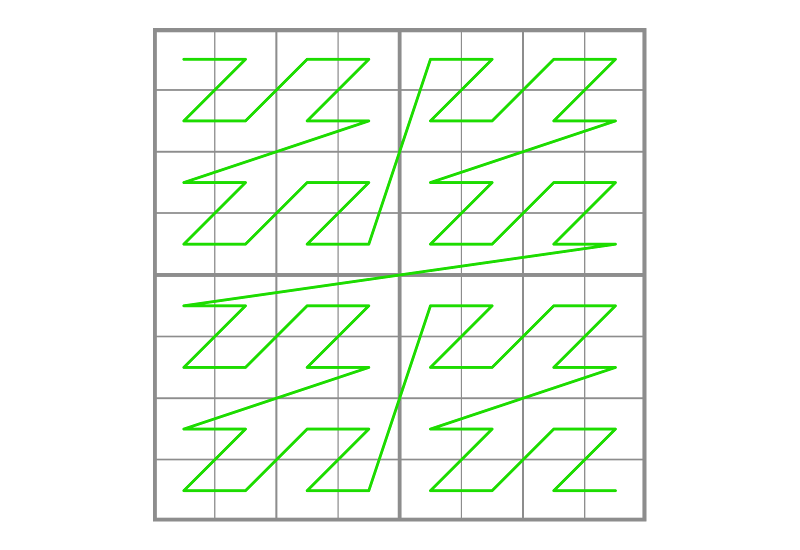
\includegraphics[width=.95\linewidth]{img/02/ZCurve.png} 
        \caption[Courbe de Morton]{Principe de la courbe de Morton.
        Ce type de courbe est mieux adaptée à l'utilisation de \ac{GPU} que la courbe de Hilbert.
 		\label{fig:hilbert}}
\end{figure}



%optimisation matérielle -> les prochaines générations de GPU


%est de séparer la gestion de l'arbre de la physique.
%La plus prometteuse semble être de supprimer complètement les copies en plaçant la totalité de l'arbre directement sur la carte.
%Le CPU étant tres efficace pour ce genre d'opération, il semble

%Copies asynchrones

\section{Gestion des entrées/sorties}
\label{sec:io}

Durant ma thèse la simulation CoDa I AMR (voir partie \ref{sec:CODAEMMA}) a été réalisée avec EMMA.
Cette simulation fait partie des plus grosse simulation de la réionisation exécutée à l'heure actuelle avec un nombre de particules de matière noire, et donc une grille de base, de $2048^3$ éléments.
Ces données devront être stockées et écrites sur disque dur or si l'on se réfère à la table \ref{tab:debits} on observe que les débits d'accès disques font partie des débits les plus faibles.

Pour se faire une idée de la quantité de données en jeu faisons une estimation : 

\begin{itemize}
\item Pour les particules:
En considérant qu'un flottant est codé sur 4 octets, chaque champs représente $2048^3 \cdot 4 = 32$Go.
Comme il y a une dizaine de champs en sortie (3 positions, 3 vitesses, etc) les particules représentes environs $320$Go par pas de temps.

\item Pour la grille :
En considérant que la quantité de cellules peut être multipliée par 3 à cause du raffinement, chaque champ (densité, température, vitesse, etc..) représente environ $32 \cdot 3 \approx 100$Go.
Il y a au total un cinquantaine de champs calculés à l'exécution de la simulation mais en pratique environ une vingtaine en sortie.
Chaque écriture de la grille représente donc $100\cdot 20 =2$To.

\item Pour les étoiles:
C'est très variable car dépend directement du nombre d'étoile à l'instant donné, qui dépend lui même du paramètre de résolution en masse.
\end{itemize}

Ce qui représente au total environ 2,3 To de données générées par pas de temps de sortie.
Mais on voudrait évidemment avoir accès à l'état de la simulation à différents instant, cette simulation a au final écrit 170 pas de temps, représentent au final un volume de données de près de 400 To.
%De plus, ces données sont stockées sur \ac{HDD}, et si l'on se réfère à la table \ref{tab:debits} on observe que les débits d'accès disques sont les plus faibles.
Étant donné la quantité de données en jeu, une bonne gestion des Entrées/Sorties peut donc permettre un gain de temps appréciable.
De plus, ces données sont généralement calculées sur des machines distantes et améliorer leur compacité peut permettre de gagner du temps au moment du transfert vers des machines locales, ou simplement au moment de la lecture pour analyse.

%Les entrées/sorties sont des étapes relativement longues et l'écriture sur disque d'une telle quantité de données demande du temps et ralentit l'exécution de la simulation.
% leurs rapatriement sur des machine locales peut également être coûteux en temps.
%Il a fallu plusieurs mois pour rapatrier localement les données générées par la simulation CODA.
%Il a fallut plusieurs mois pour rapatrier les données de CODA de TITAN aux états unis vers Strasbourg
%De plus améliorer la compacité des données permet également de gagner du temps au moment du transfert vers des machines distante, ou simplement au moment de la lecture
%analyse a distance
%le feedback CODA\\
%grosse quantité de données\\

Dans l'ancien modèle de données d'EMMA, l'intégralité de l'octree était écrit (cf figure \ref{fig:data}).
Les OCTs étaient écrit les uns à la suite des autres avec toute l'information qu'ils contenaient.
L'information étaient exacte et complète, mais le volume de données était considérable.
De plus chaque processeur écrivait un fichier indépendant, ce qui pouvait rapidement faire exploser le nombre de fichiers et être problématique selon le système de fichiers des calculateurs car il est possible d'avoir une limite sur le nombre de fichiers par utilisateur.

Dans la même optique que ce qui a été abordé dans la section \ref{sec:cpugpu}, j'ai mis en place un modèle visant à manipuler les données avant leurs transferts.
L'objectif est de sortir les données de l'arbre en se basant sur une notion de tableau de champs pour faciliter leurs traitement.
Dans ce nouveau modèle, seules les feuilles (les cellules non raffinées) sont écrites sur le disque, ce qui permet de réduire le volume et la redondance des données.

Les champs sont maintenant traités individuellement (cf figure \ref{fig:data}) et il est possible de choisir de les écrire ou non en fonction des besoins.
Les champs sont séparés dans des fichiers distincts, et les processeurs écrivent conjointement dans le même fichier grâce à l'utilisation de la librairie HDF5.
Le nombre total de fichiers ne dépend plus du nombre de processeurs sur lequel a tournée la simulation.
Et lors d'un transfert entre machines, il est possible de ne rapatrier que les données nécessaires, et ainsi économiser du temps et de la bande passante.

Malgré la quantité de données réduite, le temps passé dans la fonction de sortie n'en est que très peu affecté.
Le gain réalisé au moment de l'écriture est compensé par la charge de calculs supplémentaires due à l'extraction des données de l'arbre.
Par contre un gain appréciable est réalisé au moment de l'analyse des données.

\begin{figure}
        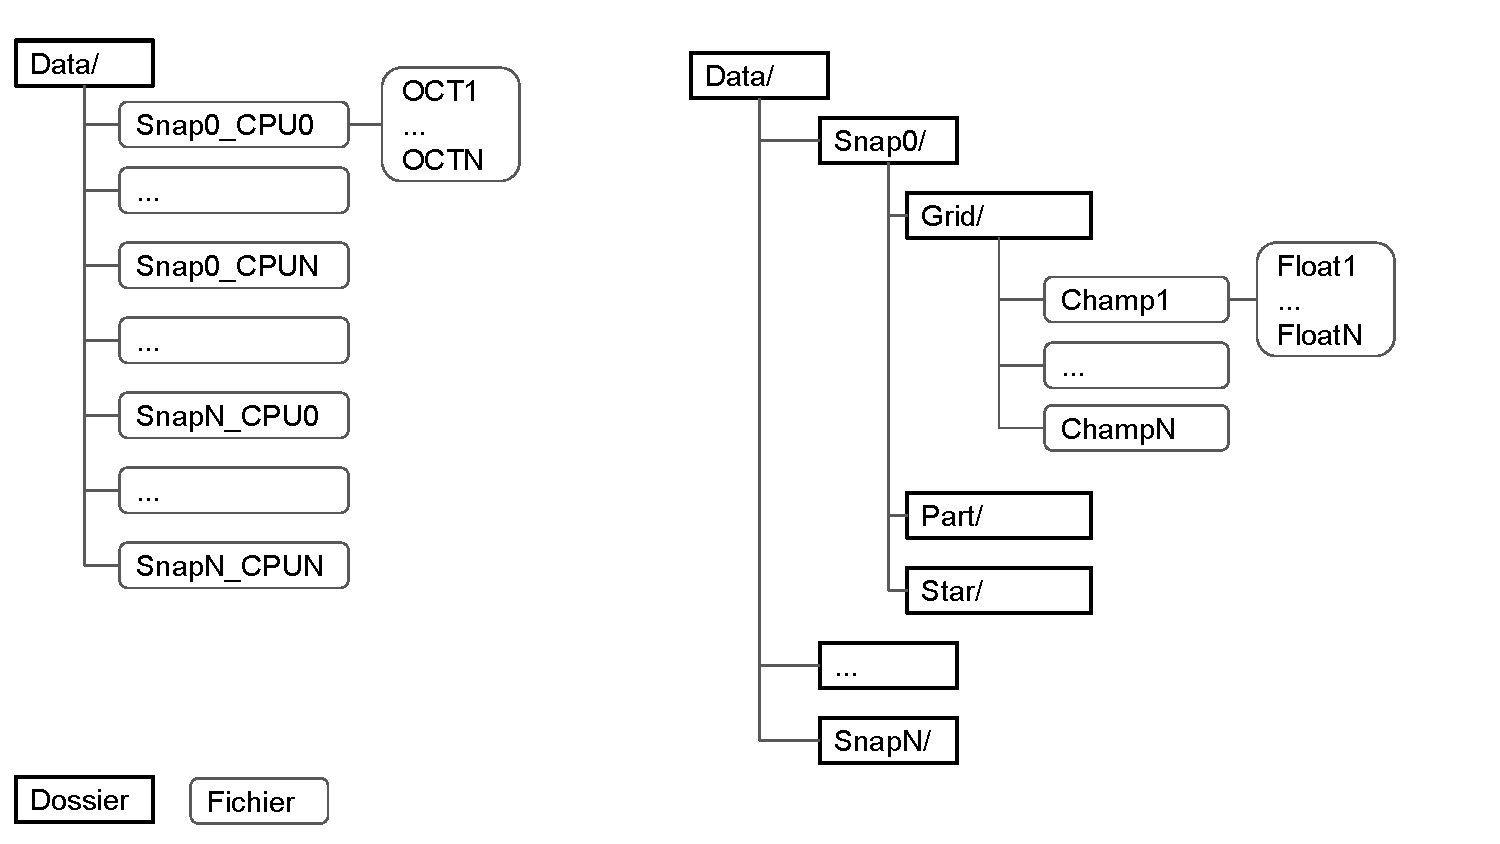
\includegraphics[width=.95\linewidth]{img/02/data.pdf} 
        \caption[Gestion des IO]{Différence entre ancienne gestion des données à gauche et nouvelle version à droite.
        Une meilleur hiérarchisation facilite l'accès aux données .
 		\label{fig:data}
 		}
\end{figure}


%En contrepartie, il est nécessaire de reprojeter la grille dans le cas d'une analyse sur un niveau intermédiaire.

%Chaque cellule est considérée comme une particule d'une certaine taille.

%Architecture des données 
%conception d'une organisation des données
%séparation des champs
%structure imposé par la gestion de l'AMR
%écriture parallèle

%\subsection{Potentiel d'optimisation EMMA}
%
%la forme des gathers/scatter
%optimisation matérielle -> les prochaines générations de GPU
%Opérations coarse sur grille non AMR.
%reformatage de l'arbre et découplage de la physique




%%%%%%%%%%%%%%%%%%%%%%%%%%%%%%%%%%%%%%%%%%%%%%%%%%%%%%%%%%%%%%%
%%%%%%%%%%%%%%%%%%%%%%%%%%%%%%%%%%%%%%%%%%%%%%%%%%%%%%%%%%%%%%%

%%\cleardoublepage
%\ctparttext{Cette partie est liée a la publication présentée en annexe\,\ref{pap:feedback}.\medskip
%
%\emph{"Radiation and supernovae feedback during the epoch of reionization with EMMA"} \medskip
%
%Nicolas Deparis, Dominique Aubert, Pierre Ocvirk et Nicolas Gillet.
%Soumis à MNRAS.
%
%\vspace{1cm}
%Ainsi qu'au proceeding de conférence présenté en annexe\,\ref{pap:feedback_proceeding}.\medskip
%
%\emph{"Stellar feedback during the reionization with EMMA"} \medskip
%
%Nicolas Deparis.
%SF2A-2016.
%
%}
%\part{La composante stellaire}
%\chapter{Mise en place d'un modèle de formation et d'évolution stellaire}
\label{sec:etoiles}

Dans les parties précédentes nous avons rapidement présenté quelles étaient les différentes physiques à l’œuvre dans les simulations de la réionisation et la façon dont elles sont modélisées numériquement.
Il manque encore une composante essentielle au problème qui est la modélisation des sources de rayonnement ionisant.
L'objectif de cette section est d'exposer le modèle de sources que j'ai développé, implémenté et calibré.
Comme nous avons vu en introduction (cf section \ref{sec:introreio}), il existe deux types de sources, les étoiles et les quasars.
Dans la suite de cette étude, je n'ai considéré que la partie stellaire sans me préoccuper des quasars.
Dans cette section je vais présenter le modèle de formation stellaire que j'ai implémenté dans EMMA.
Dans ce modèle, la formation stellaire a lieu en trois temps.
Nous allons définir les différentes phase de la vie d'une étoile, et ses différentes évolutions possible.
Il faut d'abord localiser les régions de formation, puis calculer la quantité d'étoiles à former, et enfin former les particules.
Nous verrons comment les contraintes imposées par les échelles cosmologique que l'on cherche à étudier vont imposer certains choix au niveau numérique.
Une attention particulière sera mise sur la modélisation des supernovae, puisque une étude comparative entre deux modèles d'injection d'énergie suivra.
Lors de cette comparaison, il s'est avéré que dans nos modèles, les supernovæ étaient capable de réguler le \ac{SFR}, sans changer l'histoire de la réionisation.

%\section{Les différentes phases de la vie d'une étoile}
%
%L'objectif est ici de définir les différentes phases de la vie d'une étoile.
%Nous allons aborder sa naissance, sa vie et sa mort de manière générale dans un premier temps.
%Et nous verrons ensuite l'implémentation de ces trois phases dans EMMA.

%\section{Modèle sous grille et population stellaire}

\section{Considérations de résolution}
%En fonction des echelles de travail, nous considererons soit les etoiles individuelles soit une population stellaire.

Une des difficulté majeurs dans les simulations de la réionisation, est l'impossibilité d'obtenir des résolutions suffisante pour suivre la formation des sources de radiation individuellement, tout en simulant un volume suffisamment important.
%Il existe toujours ce conflit en réionisation entre simuler des grands volume, et obtenir la meilleur résolution possible.
Actuellement les simulations capables de suivre un volume d'Univers de l'ordre de $(100Mpc)^3$ atteignent un résolution de l'ordre du kilo-parsec.
Or les échelles de formation stellaire sont de l'ordre de l'unité astronomique, soit un facteur $\approx 10^8$ plus petit.
Il est donc actuellement impossible de résoudre les deux cotés du spectre d'échelles spatiales.
%de suivre la formation des étoiles individuellement.
Il est nécessaire de créer un modèle qui va tenter de prendre en compte au mieux la physique non résolue.
Ce type de modèle est appelé modèle \textit{sous grille}.
Dans le cas présent le modèle sous grille consiste à transformer une partie du gaz en particule stellaire, cette particule ne représentant pas une étoiles mais une population stellaire de manière statistique.
%On appelle ces particules des particules puits.
Toute la difficulté du modèle de formation stellaire sera de déterminer la façon dont est réalisée cette conversion.
Malgré tout, nous verrons qu'il est possible d'obtenir un modèle statistiquement viable à grandes échelles assez facilement.

% Un second type de modèle intervient au moment de l'explosion en supernovae.
% Les processus de diffusion de l'énergie libérée aux échelles plus petite que la grille sont complexe et il en résulte une série de paramètres libres assez conséquente.

%lien entre les différents solveurs en fonction du stade évolutif
%Les étoiles se trouvent aux centre de la simulation.
%En effet, créer une étoiles consiste a transformer une partie du gaz en particule.
%Cette particule sera ensuite gérée par le solveur Ncorps, et servira de source au solveur radiatif.
%Puis a la fin de sa vie, l'étoile va injecter de l'énergie dans le solveur hydrodynamique.
%Une particule stellaire va donc devoir interagir avec tout les solveurs du code.

%Seul la partie du spectre capable de ioniser l'hydrogène est considérée. E>13.6eV



\section{La formation stellaire}

\subsection{Critère de Jeans}

%lien avec la densité\\
%Formation dans l'H moléculaire mais pas dans les simu

Les étoiles se forment au sein de nuage de gaz, par effondrement gravitationnel.
Si les conditions sont réunies, cet effondrement ne s'arrête quand les réactions thermonucléaire s'enclenchent et que le gaz forme une étoile.
En première approximation, un nuage de gaz s'effondre, si le temps de chute libre : 
\begin{equation}
t_{ff} =  \sqrt{\frac{3\pi}{32G\rho_g}} \propto \frac{1}{\sqrt{G \rho}},
\label{eq:tff}
\end{equation}
est supérieur au temps de réaction à une perturbation.
Considérant que cette perturbation est d'origine mécanique, le temps de réaction sera équivalent au temps de traversée du nuage par une onde sonore :
 \begin{equation}
t_{sound} = \frac{R}{C_s},
\end{equation}
avec $R$ la taille du nuage et $C_s$ la vitesse du son dans ce nuage.
Si le temps de réaction est plus long que le temps de chute libre
\begin{equation}
t_{ff} < t_{sound},
\end{equation}
alors le milieu n'a pas le temps de résister et le nuage s'effondre sur lui même.

$t_{ff}$ fait intervenir la densité, plus le milieu est dense plus il aura tendance à s'effondrer sur lui même.
Et de l'autre coté intervient aussi la vitesse du son $C_s$, elle même dépendante de la température $C_s \propto \sqrt{T}$.
Plus le gaz sera chaud, plus le nuage va résister a son effondrement.
%\subsection{Population III}
%tres peu de ligne de refroisdissment
%étoiles plus grosse
% temps de vie court
A haut redshift, au moment de l'apparition des premières étoiles, les métaux étaient très peu disponible (voir :\ref{sec:nucleosynthese_primordiale}).
De ce fait, le gaz disposait de relativement peu de possibilité de refroidissement, menant à une température plus élevée.
Les étoiles primordiales devaient donc être plus grosses que les étoiles de notre voisinage (plus de $100M_\odot$).
Ce type d'étoiles est appelées étoiles de population III ou popIII.

%La nucléosynthèse primordiale a créer peu de métaux. 
%A haut redshift, les metaux etaient peu disponible.
%les métaux permettent une meilleur emmission radiative, et donc un meilleur refroidissent.
%si le refroidissment est meilleur, l'equilibre hydrostatique penche an faveur de plus grosse étoiles.
%POPIII, IMF top Heavy, étoiles  primordiales
%
%plus un étoiles est grosse, plus son spectre sera énergétique et plus la portion de spectre ionisant sera important.




\subsection{Localisation des zones de formation stellaire}

Il est admis que les étoiles se forment dans les nuages d'hydrogène moléculaire (voir eg \cite{krumholz_universal_2012}).
Ces nuages se trouvent eux même dans des zones suffisamment denses pour que des molécules puissent se former.
En pratique dans EMMA, la physique de l'hydrogène moléculaire n'est pas encore prise en compte, et les zones autorisées à former des étoiles sont localisées à l'aide d'un seuil en densité.
Toutes les cellules plus dense qu'un certain seuil sont autorisées à créer des particules stellaire.

%Seuil en densité \\
\begin{equation}
	flag = 
  \begin{cases}
      True, & \text{if } \rho > \rho_{thresh}\\
      False,              & \text{otherwise}
  \end{cases}
\end{equation} 

Ce type de critère est utilisé par la grande majorité des codes de simulations cosmologique \citep{kay_including_2002}.
Cette densité de seuil $\rho_{thresh}$ peux être définie arbitrairement, et comme toute densité, elle est dépendante de la résolution.
De plus il en possible de définir une densité en unité physique ou en unité commobile (voir section \ref{sec:supercomobil}).
Un seuil en densité physique sera plus représentatif de se qui se passe réellement.
Mais à haut redshift, la densité était importante en tout points, et un seuil en unité comobile est utile pour limiter l'apparition des premières étoiles à un redshift donné.
En pratique on pourra définir ces deux seuils, et le seuil final sera le plus contraignant des deux.

%TODO figure du seuil en fonction du redshift

\begin{equation}
	\rho_{thresh} = max\left(  \delta_{in} \bar{\rho}, \rho_{in} a^3 \right)
\end{equation} 

ou $\delta_{in}$ et $\rho_{in}$  sont respectivement les paramètres de surdensité et de densité physique.
$\delta_{in}$ est exprimé en unité comobile et est donc constant dans le temps en unités du code,
 $\rho_{in}$ est exprimé en unité physique (en atome par mètre cube), sa valeur évolue dans le temps du point de vue des unités du code (cf section \ref{sec:supercomobil}).

% determination de la valeur de 55\\ 
%TODO quells valeurs sont prisent et pourquoi?

\subsection{La loi de schmidt-kennicut}
\label{sec:schmidt-kennicut}
 %conversion densité surfacique vers densité 3D\\
%rho 1.5\\
%temps de free fall\\

Maintenant que nous avons définis où former des étoiles, il nous faut calculer la quantité à former.
La loi de Schmidt \citep{1959ApJ...129..243S}  est une loi observationnelle qui lie la densité surfacique de gaz dans les galaxies au taux de formation stellaire (\ac{SFR}) dans cette galaxie.
\cite{1998ApJ...498..541K} a utilisé un modèle de galaxie pour dé-projeter la densité surfacique observée et ainsi déterminer une loi qui lie le \ac{SFR} à la densité volumique de gaz.
Cette loi a la forme:
\begin{equation}
SFR \propto \rho ^{\alpha},
\end{equation}
avec $\alpha \approx 1.4 \pm 0.15$

Le taux de formation stellaire s'exprime généralement en $M_\odot \cdot cMpc^{-3} \cdot yr^{-1}$  
Ce qui est homogène à une densité divisé par un temps.
En pratique divisera $\rho_g$ la densité locale de gaz par le temps de chute libre (equation \ref{eq:tff}), qui est en théorie le temps nécessaire à un nuage de gaz pour s'effondrer si il n'y avait aucune résistance.
Au final, le \ac{SFR} prend la forme:
\begin{equation}
	SFR = \epsilon_{sf} \frac{\rho_g}{t_{ff}} \propto \rho_g^{1.5}
    \label{eq_sfr}
\end{equation}
avec  $\epsilon_{sf}$ le paramètre d'efficacité de formation stellaire.
Observationellement, $\epsilon_{sf}$  est de l'ordre du \%. %TODO ref
Ce qui signifie que la formation stellaire est relativement inefficace.
Il est également possible de considérer le temps caractéristique de formation stellaire:
\begin{equation}
t_{sf} =  \frac{t_{ff}}{ \epsilon_{sf} },
\end{equation}
qui est de l'ordre de quelques milliards d'années.



\subsection{Implémentation}

A partir du taux de formation, on obtient la masse de gaz à convertir en étoiles dans chaque cellule en multipliant par $dv$ le volume de la cellule en question et $dt$ le pas de temps entre deux passage dans la fonction de formation stellaire:
\begin{equation}
	M_{star} = SFR \cdot dv \cdot dt .
\end{equation}

%resolution en masse\\
Nous avons donc à ce stade la masse totale de gaz à convertir en étoile.
Il devient rapidement coûteux de générer pour chaque cellule éligible, et à chaque pas de temps, une nouvelles particule stellaire (le nombre de particule peux rapidement exploser).
Nous adoptons une approche probabiliste.
Nous définissons une masse d'étoiles $m_{star}$ qui correspondra à notre "quanta stellaire".
Toutes les étoiles aurons donc la même masse et cette masse est calculée d'une manière comparable à celle d'une particule de matière noire.
La masse d'une étoile correspond à la masse moyenne de gaz dans une cellules d'un certain niveau :
\begin{equation}
 m_{star} = M_{DM} \frac{\Omega_b}{\Omega_m}\cdot 2^{-3L},
\end{equation}
où $L$ peux varier du niveau de base à niveau plusieurs niveaux raffinés.

Le nombre de quanta à ajouter est ensuite tiré aléatoirement dans une loi de Poisson \citep{rasera_history_2006}.
\begin{equation}
	P(N) = \frac{\lambda^N}{N!} e^{-\lambda}
\end{equation}

Où $\lambda$ correspond au nombre de particules moyen à créer dans la cellule :
\begin{equation}
\lambda = \frac{ M_{star}}{m_{star}}
\end{equation}
On obtiendra au final $N_{star}$ le nombre de quanta de masse d'étoiles à créer.
Étant donné le grand nombre de tirage cette loi est en moyenne valide.

En pratique j'ai implémenté deux méthodes de transformations.
Si  $N_{star}>1$ il est possible de créer : 
\begin{itemize}
\item  $N_{star}$ particules aillant chacune une masse  $m_{star}$.
\item une seule particule de masse  $N_{star} \cdot m_{star}$.
\end{itemize}

Dans le premier cas le nombre de particules sera plus élevée et la résolution stellaire meilleure, mais en contrepartie le coût numérique sera plus important.
Le choix de la méthode est laissé à l'utilisateur et dépend de la situation.
Dans tout les cas la masse nouvellement convertie est retirée de la cellule.


%En pratique la création d'une particule stellaire consistera a 
%\begin{itemize}
%\item prendre dans la réserve, une nouvelle particule %un maillon de la liste chainée
%\item ajouter ce nouveau maillons a la liste chainée de particule de la cellule.
%\item initialiser cette nouvelle particule avec : 
%\begin{itemize}
%\item un état
%\item un temps de création
%\item une vitesse 
%\item une masse
%\item un identifiant
%\end{itemize}
%\end{itemize}

%TODO resolution masse stellaire
%TODO conservation de la masse

\subsection{Quelques détails techniques}

En pratique la création d'une particule stellaire consistera à prendre une nouvelle particule vierge dans la réserve (cf section \ref{sec:PART}), ajouter ce nouveau maillons à la liste chaînée de particule de la cellule et initialiser cette nouvelle particule.

On associera un instant de création à la particule stellaire et non un age, ceci permet de ne pas avoir à remettre à jour cette valeur à chaque pas de temps.
Pendant les analyses post-simulations, on prendra garde à définir l'age des étoiles comme étant l'instant associé au snapshot courant moins l'instant de création de la particule.

Les étoiles créées auront une vitesse correspondant à la vitesse du gaz au moment de leurs création.
Pour éviter les effets de "collier", à cette vitesse sera ajoutée une composante aléatoire, aillant une direction aléatoire et une amplitude aléatoirement comprise entre $\pm c_s$ la vitesse du son dans la cellule \citep{rasera_history_2006}.

Il est utile d'associer un identifiant unique aux nouvelles particules pour pouvoir suivre leurs évolutions et les retrouver entre les différentes sorties.
La technique la plus simple est d'associer la valeur d'un entier que l'on incrémente à chaque création d'une nouvelle particule.
Du fait de la parallélisation cette incrémentation demande des communications à chaque création de particule.
Pour minimiser les communications, la pratique retenue consiste à former toutes les particules de toutes les processus, en leur assignant un identifiant caractéristique (eg -1) et d'assigner les identifiants finaux dans un second temps.
Une fois les particules créées, chaque processus compte son nombre de nouvelles particules et le transmet aux autres, ce qui permet d'allouer une plage d'identifiants par processus, et ainsi allouer les identifiants finaux.


%\begin{figure}
%        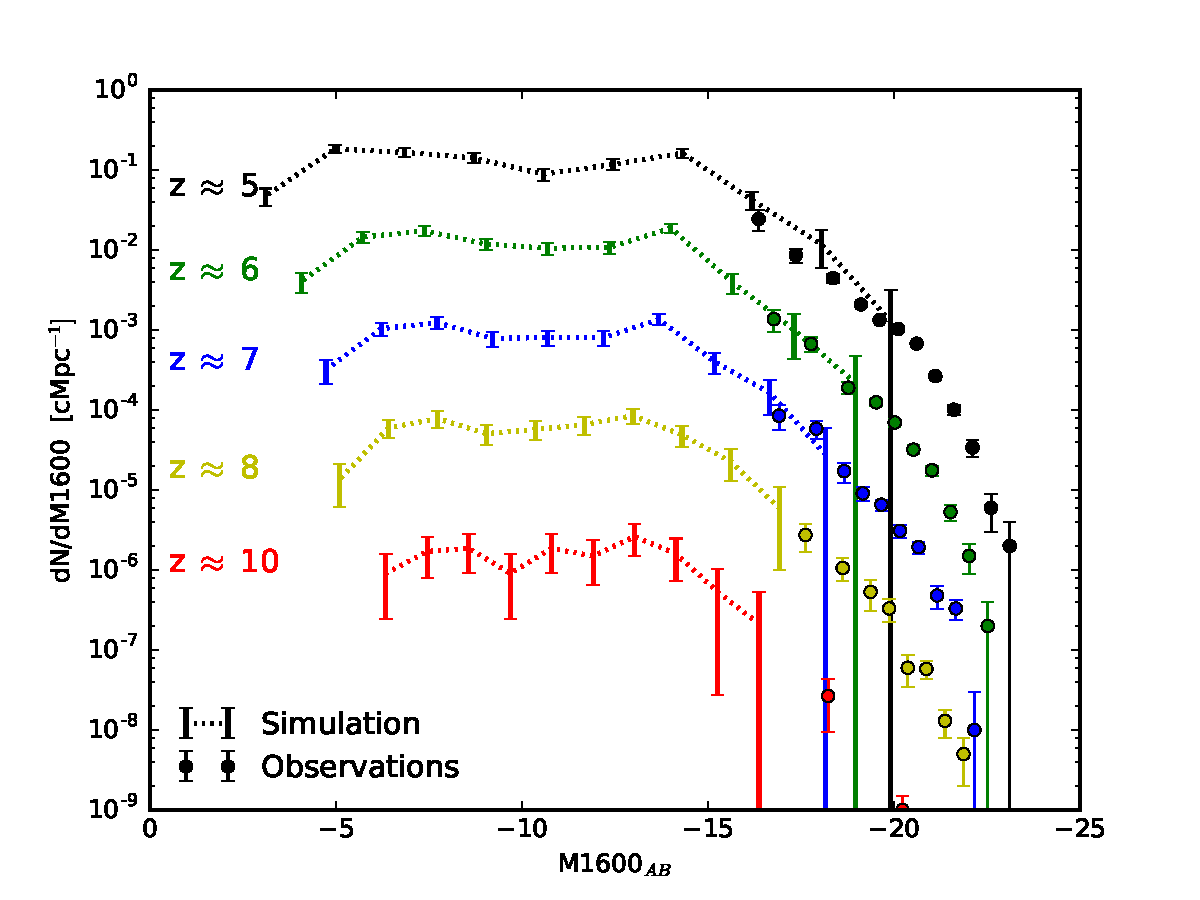
\includegraphics[width=.95\linewidth]{img/02/luminosity_function.pdf}
%        \caption{Fonction de luminosité dans la bande $M_{1600}$.
%}
% 		\label{fig:test_SFH}
%\end{figure}

%Des test plus poussés seront développés plus loin.

%\clearpage
\section{La vie radiative}
\label{sec:etoilerad}

%\subsection{Vie}
%le diagram HR

Une fois le nuage de gaz effondré et les réactions thermonucléaires amorcées, l'étoile amorce sa séquence principale.
C'est la phase qui représente la majeure partie de la vie d'une étoile.
Elle consiste en un équilibre hydrostatique entre gravitation et pression interne, maintenue par les réactions de fusion nucléaire.
L'étoile va consommer son hydrogène pour résister à l'effondrement gravitationnel, il en résultera une formation d'hélium.
%develloper le cycle proton proton ?
L'équation simplifié du processus de fusion, appelé cycle proton-proton (PP) est :
\begin{equation}
4p \leftrightarrow He^4 + 2e^+ + 2\nu + E.
\end{equation}

Plus une étoile est grosse plus le taux de réaction doit être élevé pour lutter contre la gravité.
Il en résulte que les grosse étoiles sont plus énergétique, et émettent donc plus de rayonnement ionisant.
En contre partie, ce taux de réaction élevé mène à une durée de vie plus courte.
Du fait de leurs masses, les popIII, émettaient un fort rayonnement ionisant, et avaient une vie relativement courte.

%materiaux de base est l'hydrogene\\
%plasma donc hydrogène ionisé 


\subsection{Fonction de masse Initiale}

Les étoiles naissent en groupe, et toutes ne sont pas identique.
Pour caractériser cette diversité, il existe la notion de fonction de masse initiale (\ac{IMF}), qui exprime la probabilité de former une étoile d'une certaine masse dans un population.

\begin{equation}
A_{(M)} = a_0 \cdot m^{-\alpha}
\end{equation}

Parmi les \ac{IMF} plus connues il y a :

\begin{itemize}
\item \cite{1955ApJ...121..161S}
\item \cite{1979ApJS...41..513M}
\item \cite{2001MNRAS.322..231K}
\item \cite{2003PASP..115..763C}
\end{itemize}

Chacune d'elles présentant des pentes $\alpha$ différentes, et certaine avec plusieurs intervalles.
%TODO Quelles sont les différences

%Comme nous l'avons abordé plus haut, les étoiles de population III avaient tendance a être très massive.

Des travaux comme \cite{2003MNRAS.344L...7C} suggère que lors de la réionisation, il y avait formation d'une forte proportion d'étoile massive, j'ai donc utilisé par la suite une \ac{IMF} Top-Heavy avec les caractéristiques suivantes :

\begin{equation}
	\alpha = 
  	\begin{cases}
	1.3 & si 0.1 < m/M_\odot \leq 0.5\\
	2.3 & si 0.5 < m/M_\odot \leq 1 \\
	1.6 & si 1   < m/M_\odot \leq 100 \\
	\end{cases}
\end{equation} 

%: difficulté a reioniser avec Salpeter -> passage a top heavy -> justification 
%Fonction de masse IMF Top Heavy

\subsection{Starburst99}
\label{sec:staburst}
%Pour modeliser 
%paramètre d'entrée
%sorties

Une fois les étoiles formées, il est nécessaire de les faire rayonner.
Pour ce faire il faut, à partir de leurs masses et de leurs ages, calculer leurs émissivité.
Pour déterminer quel est le lien entre age, masse et luminosité d'une particule stellaire on utilisera un modèle de population stellaire.


Les étoiles d'une population ayant des masses et des évolutions différentes, l'émission résultante sera la somme des contributions individuelles.
La modélisation de population stellaire est complexe, et il existe différent modèles dédiés à cette tache.
On peut citer entre autres :

\begin{itemize}
\item Starburst99 \cite{leitherer_starburst99:_1999} 
\item \cite{2003MNRAS.344.1000B}
\item FSPS \cite{2009ApJ...699..486C}
\end{itemize}

A partir d'informations caractéristiques d'une population stellaire, comme sa masse, son \ac{IMF} ou sa métallicité, ces modèles retournent un spectre d'émission et son évolution en fonction du temps (cf Fig \ref{fig:spectre_starburst}).
Le choix a été fait d'utiliser Starburst99, car en plus des spectres, il retourne plusieurs informations utiles au modèle comme l'énergie et la masse injectées par les supernovae (section \ref{sec:sncali}).

\begin{figure}
        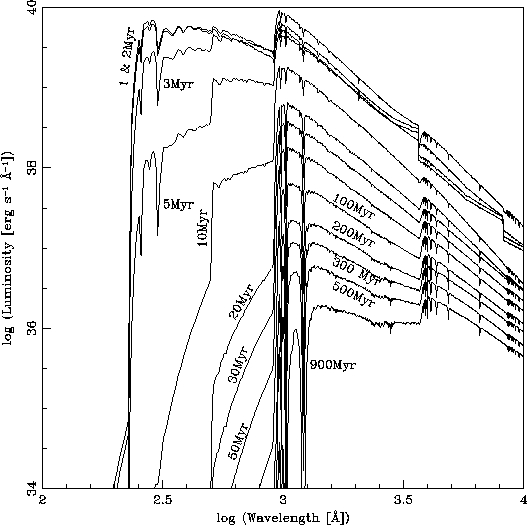
\includegraphics[width=.95\linewidth]{img/03/spectre_starburst.jpg} 
        \caption[Spectres Starburst99]{Spectre d'émission d'une population stellaire généré par Starburst99.
        Ici avec les paramètres sont $M_{pop}=10^6 M_\odot$, \ac{IMF} de Salpeter ($\alpha=2.35$ et intégration de 1 à 100 M$_\odot$ 
 		\label{fig:spectre_starburst}}
\end{figure}

%injection d'énergie dans le solveur radiatif, ok mais combien?\\
%calibration energetique et Starburst99\\

%J'ai commencé mes calibrations avec une \ac{IMF} de Salpeter, mais il s'est vite avéré que les sources n’émettaient pas assez de photons ionisant et que les boites n'arrivaient pas a reioniser.
%La majorité des simulations que j'ai réalisées ensuite utilisent une \ac{IMF} Top-Heavy.


A partir des spectres obtenus avec Starburst99 (cf section \ref{sec:staburst}), nous n'allons garder que la partie capable de ioniser l'hydrogène (toutes les longueurs d'onde plus courte que 912$\AA$) :

\begin{equation}
E_{ion (t)} = \int_{13.6eV}^{+\inf} h \nu_{(t)} d\nu
\end{equation}

En divisant l'énergie totale obtenue à partir de cette intégration, par l'énergie moyenne des photons obtenue à partir des spectres (cf section \ref{sec:groupedephotons}), on obtient l'évolution du flux de photons ionisant, présenté sur la figure \ref{fig:flux}.
\begin{figure}
        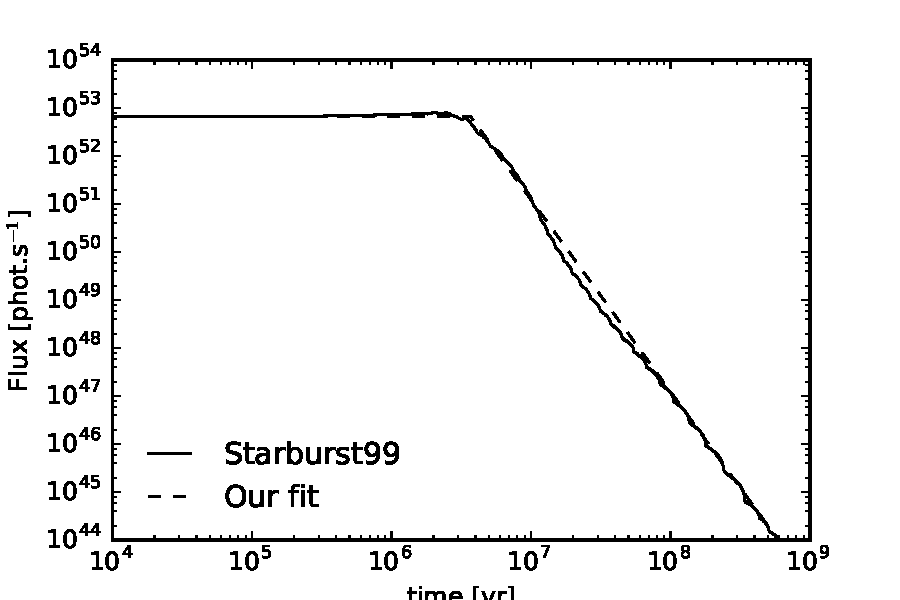
\includegraphics[width=.95\linewidth]{img/03/flux.pdf} 
        \caption[Émissivité ionisante]{Émissivité ionisante intégrée en fonction du temps.
        La population présente deux phases d'émission, une phases constante suivie d'une rapide décroissance.
 		\label{fig:flux}}
\end{figure}
Le profil obtenu présente un plateau d'émissivité constante suivie d'une rapide décroissance.
Ce profil peut être raisonnablement approximé par:

\begin{equation}
    S = 
\begin{cases}
    S_0 ,         & \text{if } t < t_{life}\\
    S_0.t^{-4},   & \text{if } t_{life} \leq t < 100t_{life} \\
    0,   & \text{if } 100t_{life} \leq t
\end{cases}
\end{equation}

où $t_{life}$ est définis comme étant l'age de la population au moment de changement de régime.
Par la suite nous utiliserons la valeur de $t_{life} = 3.7$Myrs.

Étant donné la rapide décroissance en luminosité, les étoiles sont arbitrairement éteintes après $100 \cdot t_{life}$.

Le flux obtenu correspond au flux d'une population de $10^6M_\odot$, et ces valeurs seront pondérées au prorata de la masse de la particule stellaire : une particule de $10^5M_\odot$ émettra  simplement 10 fois moins de photons ionisant qu'une population de $10^6 M_\odot$.

Cette émissivité sera ensuite pondérée par un paramètre d'efficacité.
Ce paramètre libre reflète l'impact d'une grande partie de la physique sous grille, sur le rayonnement.
En effet, nous ne résolvons pas certains processus, comme par exemple l'absorption par la poussière, qui va empêcher la radiation de sortir de l’environnement de la population.
Ce paramètre est analogue à une fraction d'échappement intrinsèque et ne doit pas être confondu avec la fraction d'échappement des galaxies que nous aborderons par la suite (voir section \ref{sec:fesc}).

Il nous reste encore à caractériser le type de photons à émettre.
La gestion des groupes de photons a été abordée dans la section \ref{sec:groupedephotons}, nous ne travaillerons par la suite qu'en émission mono-groupe.
%Les caractéristiques des photons émis dans le cas d'une \ac{IMF} Top-Heavy sont présentés sur la table \ref{tab_photon}.

%\begin{table}
%\begin{tabular}{l l }
%	$<h\nu>$	&  $23.42$ eV \\
%	$\alpha_e$	&  $2.35.10^{-22}$ m$^2$ \\
%	$\alpha_i$	&  $1.82.10^{-22}$ m$^2$ \\
%\end{tabular}
%\caption[Propriété des photons]{Propriété des photons émis par les sources.
%Ces valeurs ont été calculées à partir des spectres obtenus avec Starburst99.
%\label{tab_photon}}
%\end{table}


\subsection{Quelques détails techniques}

En pratique, il faudra calculer l'émissivité sur toute la grille.
Cette opération est simplifiée par l'utilisation de la liste chaînée de particules (cf section \ref{s}).
En effet, on passera en revue toutes les cellules, et pour chaque cellules on passera en revue toutes ses particules.
On testera alors si une particules est une étoiles (la liste chaînée contient également les particules de matière noire), et si cette étoiles est dans un stade où elle émet de l'énergie lumineuse.
Si c'est le cas, on calculera son émissivité et on injectera cette énergie sous forme de source dans l'équation \ref{eq:densite_energie}.
Le calcul de $\dot{N}_\nu^*$ sera effectué dans toutes les cellules.


%TODO intégration de l'énergie et de la section efficace


%We found a mean energy of $<h\nu> = 23.42$ eV,
%an energy weighted cross section of
%$\alpha_e = 2.35.10^{-22}$ m$^2$
%and a number weighted cross section of
%$\alpha_i = 1.82.10^{-22}$ m$^2$


%Masse de la population\\
%produit en croix pour correspondre a la masse dans simu\\
%integration seulement sur energy ionisante\\
%
%Multigroupe frequence\\
%multigroup temporel\\



%\section{Le problème de la masse des étoiles}
%
%%le paramètre de masse des étoiles change la reionization\\
%%effet numérique\\
%%le rayonnement est piégé dans les cellules\\
%
%Durant mes calibrations, il s'est avéré que le paramètre de résolution de la masse des particules stellaire avait une grande importance dans l'évolution de la fraction ionisée.
%Même si celui ci n'a pas d'impact sur la SFR globale, le taux d'ionisation moyen est fortement dépendant de ce paramètre (cf Fig .\ref{fig:mstar}).
%Plus la résolution stellaire est élevée, plus la boite réionise tard.
%Les "grosse" particules stéllaire mènent a un taux d'ionisation plus important.
%
%\begin{figure}[bth]
%        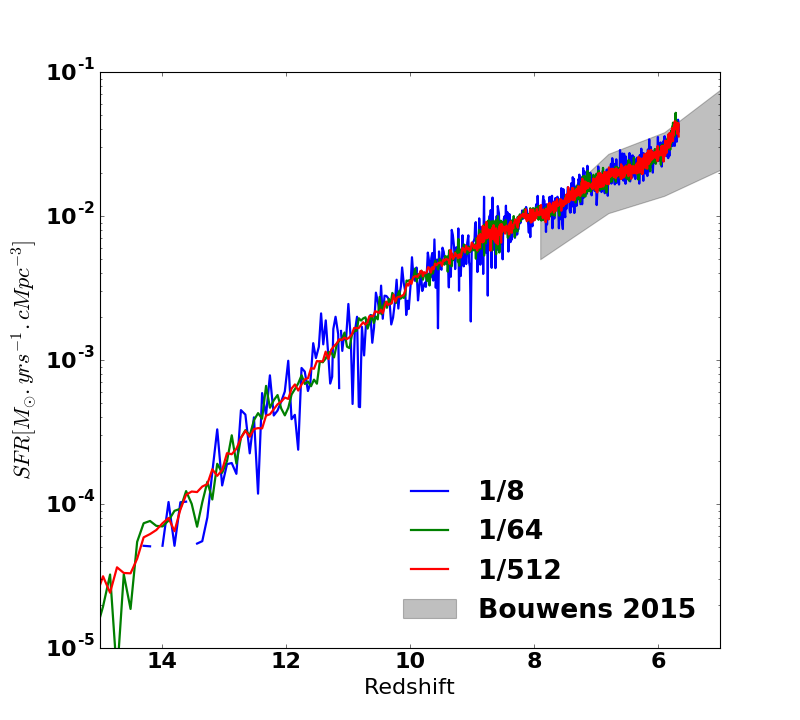
\includegraphics[width=.45\linewidth]{img/02/Mstar_SFH.png} 
%        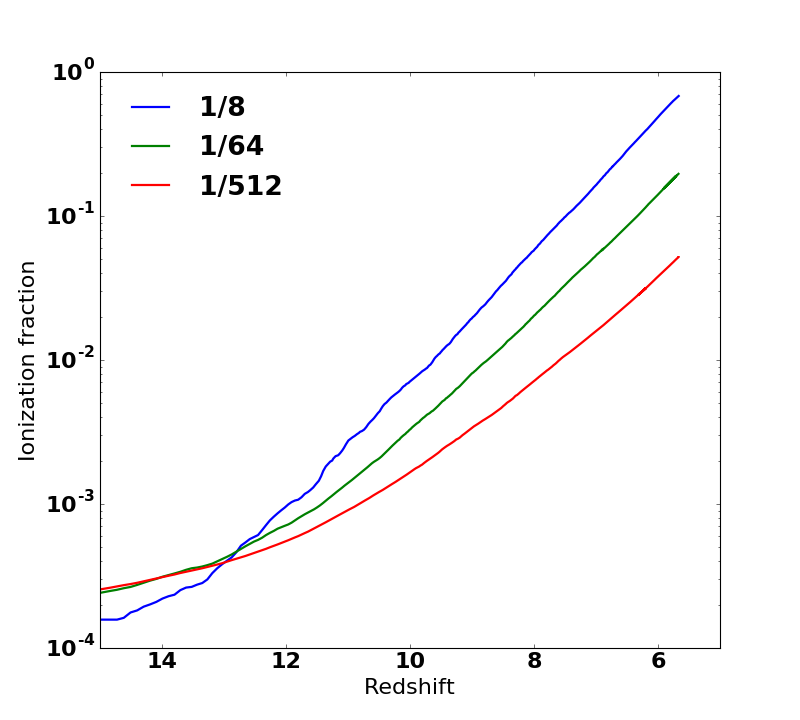
\includegraphics[width=.45\linewidth]{img/02/Mstar_xion.png} 
%        \caption{
%        En changeant le parametre de résolution en masse des particules stellaire, la SFH moyenne reste constante mais l'histoire d'ionisation s'en trouve impacté.
%}
% 		\label{fig:mstar}
%\end{figure}


%\clearpage
\section{Les supernovæ}

Dans cette section, nous allons aborder la modélisation des supernovae dans les simualtion cosmologiques.
Je présenterai deux des modèles que j'ai implémenté, ainsi que les tests numériques qui permettent de les valider.
Nous verrons que ces modèles sont équivalent dans un cas idéal mais divergent lors de l'introduction de la physque du refroidissment.
Nous aborderons également la problématique de la calibration de ces modèles.

%Il a fallut trouver un mécanisme d'introduction d'énergie dans le gaz.
%Les supernoavae ont été proposées comme mécanisme.

Les supernovae ont été introduites dans les simulations cosmologiques pour réduire l'effondrement du gaz sur lui même.
Sans l'introduction d'énergie dans le gaz par les supernovæ, le gaz s'effondre de manière importante et créer un nombre élevé d'étoiles.
Cela mène à un taux de formation stellaire trop important par rapport à ce qui est observé.
Ce problème est connus sous le nom de "overcooling problem"
L'objectif est de casser les structures pour diminuer les surdensité et limiter la formation stellaire.
Une fois que la supernovae a explosé, il en résulte une onde de choc qui va se propager dans le milieu environnant.


%\subsection{Le modèle théorique}
%Il existe principalement deux événement pouvant mener a un explosion de supernovæ : 
%
%\begin{itemize}
%\item soit l'étoile est a l'origine suffisamment massive (plus de 8Mo) pour s'effondrer a la fin de sa vie.
%\item soit l'étoile n'est pas suffisamment massive (elle va donc mourir en naine blanche) mais dispose de suffisamment de matière a proximité (généralement étoiles double ou le compagnon pas en phase géante rouge) pour que sa masse augmente avec le temps.
%la matière accreté va faire passer la masse de cette étoile au dessus de la limite.
%\end{itemize}
%
%Les étoiles de plus de 8mo exploses en SN en injectant 1e51 erg dans le milieu\\
%Cette injection limite fortement la formation stellaire dans le milieu.\\
%modèle sous grille\\

\subsection{Les différentes phases}
L'évolution du front d'onde à lieu en plusieurs phases, on en distinguera principalement deux : 

\begin{itemize}
\item Expansion adiabatique.
Dans la phase d'expansion adiabatique, l'énergie cinétique est conservée, le choc est violent et le gaz n'a pas le temps de perdre de l'énergie par radiation.
Dans cette phase, l'expansion est suffisamment rapide pour que la dissipation d'énergie par radiation soit négligeable.
%C'est par exemple le cas du test de Sedov.

\item Snowplow.
Dans la phase snowplow, le choc a suffisamment ralentis pour que le gaz commence à dissiper de l'énergie par rayonnement.
Dans ce cas, il se forme un bourrelet de compression dans lequel le gaz est poussé, comme dans le cas d'un chasse neige. 
Les pertes par radiation deviennent importantes et l'énergie cinétique n'est plus conservée.
\end{itemize}

\subsection{Les Superbubles}
%A la manière de la percolation des bulles de HII, les bulles de supernovae 

Dans les endroits de formation stellaire, les étoiles ne sont pas isolées mais apparaissent ensemble au sein d'un même nuage de gaz.
L'effondrement gravitationnel du nuage mène à créer une génération d’étoiles en un cours laps de temps.
Toutes ces étoiles vont mourir dans un laps de temps rapproché et ainsi, les différentes supernovæ vont injecter de l’énergie dans le milieu dans un laps temps rapproché.
Les différentes ondes de chocs vont se cumuler et la résultante va mener à la création d'une bulle de gaz chaud pouvant englober les galaxies.
On appelle ces régions des  superbubble.

\subsection{Considérations d'échelles}
La façon de gérer les supernovae sera donc fonction de l'échelle que l'on considère.
Dans des simulations détaillées de galaxies, il sera nécessaire de résoudre la phase adiabatique des explosions d'étoiles individuelles. %TODO ref simu de galaxie zoom
Dans les simulations cosmologiques de la réionisation qui nous intéresses ici, l’intérêt sera plus porté sur la phase snowplow des superbubbles.

%\subsection{ Différentes implémentations existantes}
%\subsubsection{Navaro and white}
%\subsubsection{Stinson et al}
%\subsubsection{dubois et Teyssier}
%Utilisation de particule fantômes pour simuler les différentes phase
%
%\subsubsection{Dalla Veccia et Schaye}
%Modèle probabiliste, injection d'énergie seulement si l'énergie est suffisante pour générer un mouvement suffisant.

\subsection{Mes Implémentations}
\label{sec:SNmodel}

\subsubsection{Modèle thermique}
Le modèle thermique consiste à injecter l’énergie de l'explosion sous forme d’énergie interne.
Il existe 2 variables d’état liées à l’énergie interne : la pression et la température.
Modifier l'une ou l'autre est équivalent et dans l’implémentation actuelle, le choix a été fait de travailler sur la pression.
Elle est modifiée de la façon suivante :

\begin{equation}
P^{0+} = P^{0-}  + E_0 \cdot  (\gamma-1)
\end{equation}

L'injection de l'énergie va donc résulter en une augmentation de la pression dans la cellule et le gaz sera mis en mouvement par conversion de l'énergie interne en énergie cinétique. 
L'avantage de cette méthode est que l'injection ne nécessite la modification que d'une seule cellule.
Cependant il est connu pour avoir de fortes pertes de d'énergie dans le cas ou le refroidissement est autorisé.

\subsubsection{Modèle cinétique}

Le modèle cinétique a pour objectif d'éviter le conversion entre énergie interne et énergie cinétique en modifiant directement cette dernière.
Le modèle cinétique consiste à modifier directement la vitesse du gaz autour de l'explosion dans le but de shunter la conversion de l'énergie interne en mouvement.
%Ce type de model a été utilisé pour 
Il n'est plus possible ici de ne modifier qu'une seule cellule.
Plus le nombre de cellules dont la vitesse sera modifiée autour de l'explosion sera important, meilleure en sera la sphéricité de l'onde choc.
Le choix a été fait de limiter le nombre de cellules utilisées à 8 correspondant a 1 oct de la structure \ac{AMR} d'\emma .
Ceci à deux conséquences.
Premièrement la recherche de voisin est réduite à l'exploration de l'OCT parent de la cellule ou a lieu l'explosion, le cout numérique est donc réduit à son strict minimum (voir section \ref{sec:voisins}).
Deuxièmement, un OCT ne peut pas être divisé entre les processeurs, ce qui assure que l'explosion a lieu au sein d'un processeur unique et permet d'éviter les communications.

En pratique l'énergie de l'explosion sera uniformément répartie sur les 8 cellules de l'OCT, ainsi chaque cellule recevra : 

\begin{equation}
e_{SN} = E_{SN}/8.
\end{equation}

Cette énergie est utilisée pour changer la vitesse du gaz de chaque cellule en utilisant : 

\begin{equation}
    \Delta \overrightarrow{v_{gas}} = \sqrt{\frac{2e_{SN}}{\rho_g.dV}} \overrightarrow{u}
    \label{eq_sn_direct}
\end{equation}

Où les vecteurs $\overrightarrow{u}$ sont les directions radiales au centre de l'OCT (cf figure \ref{fig:kin}).

\begin{figure}
        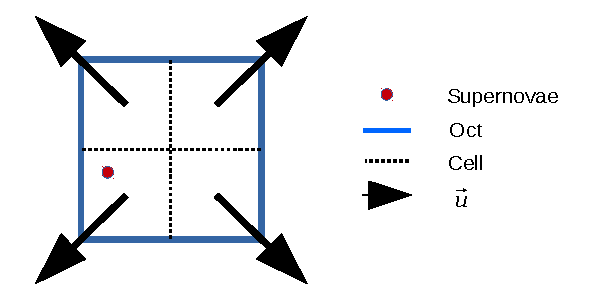
\includegraphics[width=.95\linewidth]{img/03/oct_kinetic.pdf} 
        \caption[Injection d'énergie cinétique]{Avec le modèle cinétique l'explosion a lieu au sein d'un OCT, et radialement au centre de celui ci.
 		\label{fig:kin}}
\end{figure}

\subsection{Calibration}
La quantité d'énergie injectée est calibrée en utilisant les informations en sortie de Starburst99.
Celui ci retourne également la quantité de masse perdue lors de l'explosion.
Le modèle actuel ne considère pas la possibilité d'une explosion continue, avec un retour de masse ou d'énergie s'étalant dans le temps.
L'injection est réalisée instantanément quand la quantité d’énergie théorique de Starburt99 représente 50\% de l’énergie totale.
La comparaison entre les sorties de Starburst99 et le modèle implémenté est présenté sur la figure \ref{fig:SNloss}.
Dans ce modèle, un particule stellaire injectera $9.7\cdot 10^{11} J.kg^{-1}$ et perdra 53\% de sa masse dans le milieu environant, $17.6$ millions d'années après sa formation.

\begin{figure}
        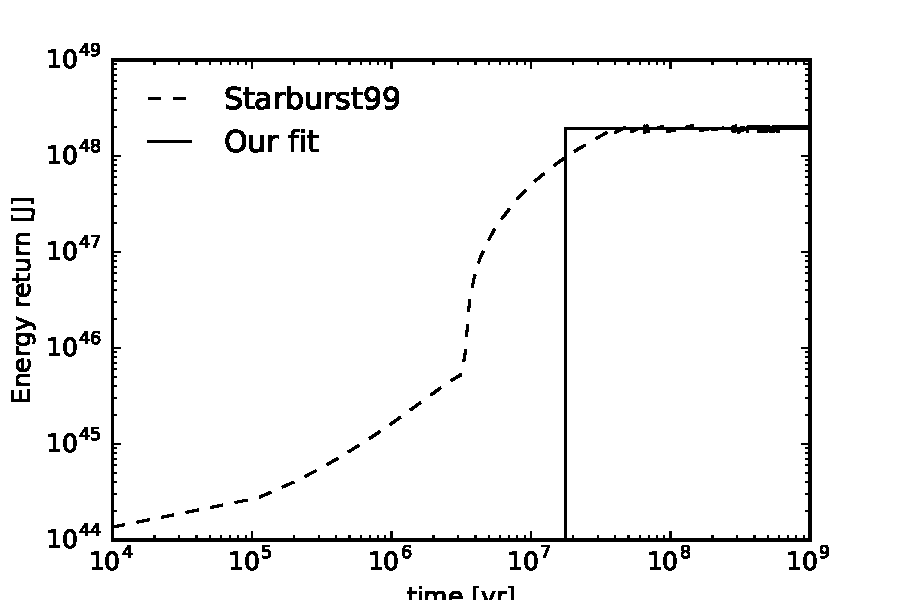
\includegraphics[width=.95\textwidth]{img/03/energy_loss.pdf} 
		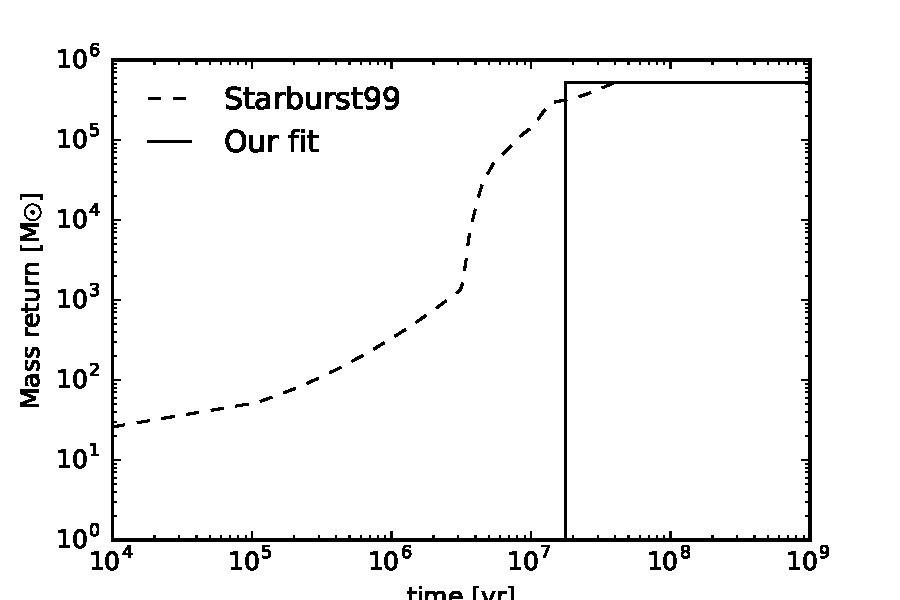
\includegraphics[width=.95\textwidth]{img/03/mass_loss.pdf} 
        \caption[Calibration des supernovæ]{ Quantité d'énergie et de masse injectés par les supernovae. Comparaison entre le modèle théorique de Starburst99 et le modèle d'injection instantané implémenté dans EMMA.
 		\label{fig:SNloss}}
\end{figure}


\subsection{Test numérique - Explosion de Sedov}
\label{sec:sedov}

%la dérivation des solutions du test de Sedov se trouve :
%chapitre 17 de Shu the physique of astrophysic Volume 2.\\

Dans le but de tester l'implémentation des différents modèles d'injection d'énergie, je les ai soumis au test de Sedov.
Ce test est utilisé pour tester le cas d'une explosion parfaite et a l'avantage de posséder une solution analytique.
Il consiste a relâcher instantanément une quantité d'énergie $E_0$ dans un milieu homogène d'indice adiabatique $\gamma$, de densité $\rho_0$ et de pression $P_0$ (ou de température $T_0$).
Ce brusque changement dans l'état du système créer une discontinuité que le solveur va devoir gérer.
\cite{sedov_similarity_1959} a exprimé le rayon de l'explosion en fonction du temps  : 

\begin{equation}
r_{(t)}=\left( \frac{E_0}{\alpha \rho_0 }\right)^{1/5} t^{2/5}
\end{equation}

%TODO expression analytique du profil

\subsubsection{Évolution temporelle }

%parametre du test :
%rho=1
%p=1e-5
%v=0
%gamma=5/3

Ce premier test consiste à injecter l'énergie dans le milieu et à suivre l'évolution du profil et de la position de l'onde de choc dans le temps.
%On s'assure alors que son profil et sa position sont correct 
%On calcul pour chaque cellule sa distance au centre de l'explosion, puis en utilisant un histogramme sur les rayons, pondéré par la valeur du champ que l'on veux analyser, on obtient rapidement le profil radial moyen.
Le résultats présentés utilisent l'injection thermique dans une seule cellule.
Le domaine de calcul est en une grille régulière décomposé en $256^3$ éléments  de calcul et le raffinement n'est pas autorisé.

La colonne de gauche de la figure \ref{fig:sedov_profil} présente les profils radiaux de densité, de pression et de vitesse radiale à trois instant différents, comparé a la solution analytique.
On observe un très bon accord entre la simulation et la théorie, l'implémentation de la méthode d'injection d'énergie thermique est donc correcte et bien dimensionnée.

\subsubsection{Comparaison des modèles}

Le test présenté ici consiste à vérifier la validité de différentes méthodes d'injection, nous allons en comparer trois : 
\begin{itemize}
\item l'injection thermique dans une cellule,
\item l'injection thermique dans un cube de huit cellules,
\item l'injection cinétique dans un cube de huit cellules.
\end{itemize}

Les trois simulations utilisent cette fois ci un espace discret de $128^3$ éléments, mais en autorisant le raffinement sur 3 niveaux.
Dans le but de concentrer le raffinement sur le front de l'onde choc, le raffinement est effectué sur le gradient de densité : une cellule est raffinée si son gradient de densité est supérieur à un seuil donné.

La colonne de droite de la figure \ref{fig:sedov_profil} présente les profils obtenus a un instant donné pour les différentes méthodes d'injection d'énergie et pour les différents champs.
On observe que le front est bien situé au même endroits indépendamment de la méthode.
Les profils sont identiques 
%Le profil de densité est présenté en échelle logarithmique pour accentuer les difference au niveau du centre. 

Même si les profils radiaux moyens sont comparables, on observe des différences sur la forme de l'explosion.
La figure \ref{fig:sedovslice} présente une coupe suivant l'axe z de la grille, contenant la cellule d'injection, pour les trois méthodes.
Ces différence sont dues a la grille et a la façon dont les flux sont calculés.
Dans le cas de l'injection thermique, les flux auront tendance à être suivant les axes principaux de la grille.
Ce qui donne ce motif en forme de "+" bien particulier.
Dans le cas de l'injection cinétique, les vitesses sont forcées à être dans des directions obliques, à 45° par rapport à la l'axe de la grille.
Nous avons cette fois si une figure en forme de "x".

Le panneau inférieur droit de la figure \ref{fig:sedovslice} présente le motif de raffinement obtenu pour le test d'injection thermique sur une cellule.
Le motif de raffinement est similaire pour les trois simulations.

\begin{figure}
   \begin{minipage}[c]{.5\linewidth}
        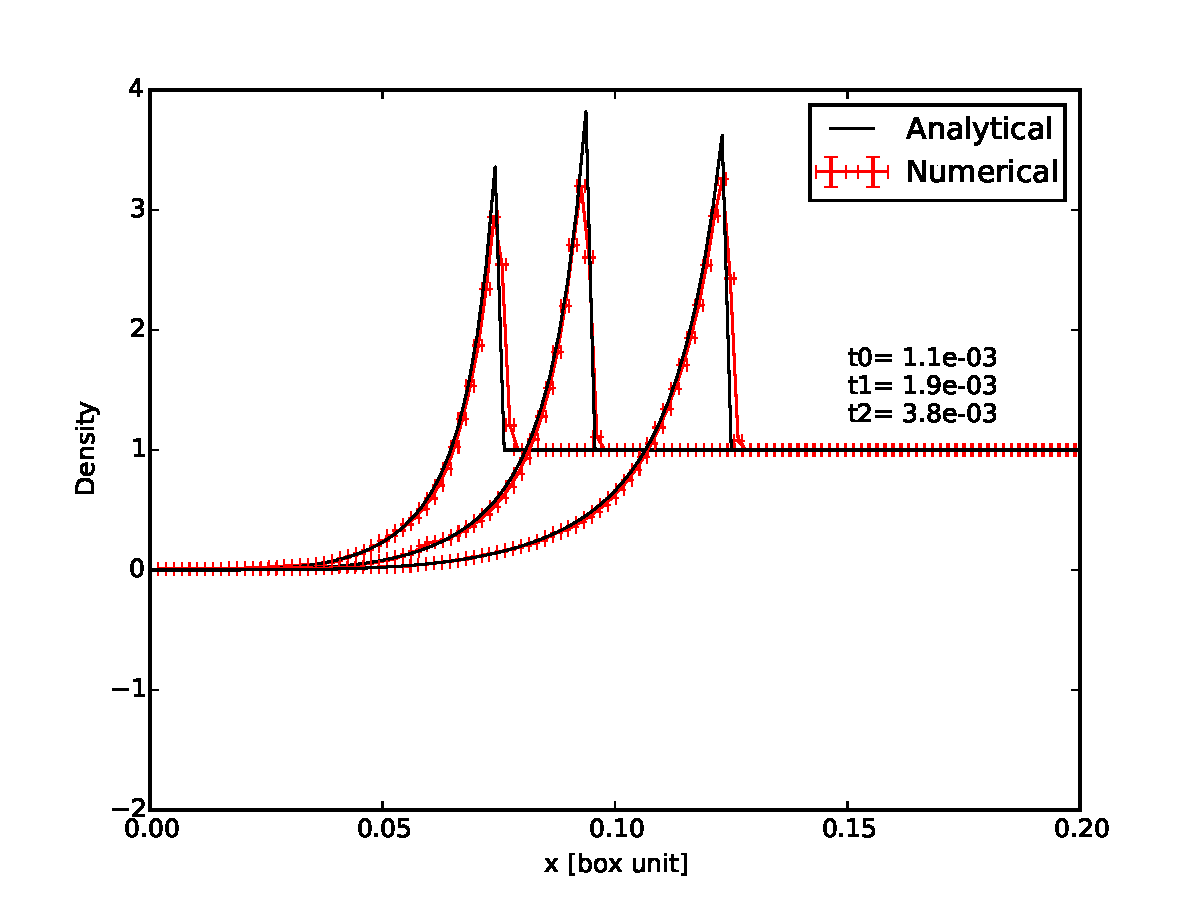
\includegraphics[width=\textwidth]{img/03/sedov/sedov_evol_8_den_lin.pdf} 
		\includegraphics[width=\textwidth]{img/03/sedov/sedov_evol_8_pres.pdf} 
		\includegraphics[width=\textwidth]{img/03/sedov/sedov_evol_8_vel.pdf} 

   \end{minipage} \hfill
   \begin{minipage}[c]{.5\linewidth}
		
		\includegraphics[width=\textwidth]{img/03/sedov/sedov_comp_profile_den.pdf} 
		\includegraphics[width=\textwidth]{img/03/sedov/sedov_comp_profile_pres.pdf} 
		\includegraphics[width=\textwidth]{img/03/sedov/sedov_comp_profile_vel.pdf} 

   \end{minipage}

        \caption[Test de Sedov - Profils]{Profils radiaux des différentes variables d'états lors du test de Sedov, . 
        La densité en haut, la pression au milieu et la vitesse radiale en bas.     
        Colonne de gauche :
        Comparaison des profils à différents instants avec le méthode d'injection thermique.
        L'accord avec la théorie est excellent.
        Colonne de droite :    
        Comparaison en fonction des méthodes d'injection. 
        La position et la forme du front d'onde ne dépendent pas de la méthodes d'injection utilisée.
 		\label{fig:sedov_profil}
 		}
\end{figure}

\begin{figure}

	\centering
	\subfloat[]{ \includegraphics[width=.45\linewidth]{img/03/sedov/slice_therm1.pdf}} 
	\subfloat[]{	\includegraphics[width=.45\linewidth]{img/03/sedov/slice_therm4.pdf}} \\

	\subfloat[]{	\includegraphics[width=.45\linewidth]{img/03/sedov/slice_kin.pdf} }
	\subfloat[]{	\includegraphics[width=.45\linewidth]{img/03/sedov/slice_th_1raf_cut.pdf}}

    \caption[Test de Sedov - Tranches]{Différents motif d'explosion en fonction de la méthodes d'injection.
    Chaque figure représente une tranche d'une cellule d'épaisseur contenant le site de l'explosion.
    (a), (b) et (c) représente le log de la densité avec une colormap quantitative.
    A cause de la grille de calcul, il existe des axes privilégiés pour les flux, il en résulte des motif en croix et ou en losange.
    La figure (d) représente les niveaux de raffinements, l'échelle est différent et le niveau 10 est aligné sur le front d'onde.
    }
 	\label{fig:sedovslice}
\end{figure}

%\subsubsection{Conclusion}
%
%La conclusion de ses tests est que les différentes méthodes d'injection sont équivalentes, au moins dans le contexte du test de Sedov.
%OK\\
%mais pas en cosmo
%le pas de temps\\

\section{Tests en conditions de production}

Dans le but de tester ces différentes méthodes d'injections dans un contexte cosmologique j'ai réalisé une série de simulations.


\subsection{Présentation des simulations}
\label{sec:pres_simu}
Chacune de ces simulation est strictement identique a l'exception de la méthode d'injection d'énergie.
Les paramètres communs a toutes les simulations qui vont suivre sont les suivants:
Elles représentes un volume de $8h^{-1}$ cMpc cube échantillonnées par $256^3$ éléments de résolutions. % particules de matière noire.
Ce qui mène à une résolution en masse de $3.4 \cdot 10^6 M_\odot$ et une résolution spatiale de $46$ ckpc sur le niveau de base.
La grille est raffinée suivant une méthode semi-lagrangienne (voir Sec. \ref{sec:raffinement}) avec une limite de résolution de 1 kpc.
Les condition initiales ont été générées avec MUSIC \citep{hahn_multi-scale_2011} avec une cosmologie de Planck \citep{planck_collaboration_planck_2016} : 
$\Omega_m=0.3175$, 
$\Omega_v=0.6825$,
$\Omega_b=0.0490$,
$H_0=67.11$,
$\sigma_8=0.830$. 
Les simulations commencent à redshift $z=150$.

\subsection{Influence de la méthode d'injection}

Le premier test consiste à essayer les différents feedback avec la même quantité d'énergie injectée, et a mesurer leur impact sur la \ac{SFH} cosmique.
La figure \ref{fig:sfr_methode} présente les résultats obtenus.
La méthode d'injection cinétique a plus d'impact en condition cosmologique.
Ceci est du à l'introduction de la physique du refroidissement.
La méthode thermique repose sur le principe de conversion de l'énergie interne en énergie cinétique.
La méthode thermique est connue %TODO ref
pour subir d'importante perte d'énergie.
La méthode cinétique outre passe cette conversion et mets directement le gaz en mouvement.

%TODO parler du feedback radiatif

\begin{figure}
        \includegraphics[width=.95\textwidth]{img/03/sedov/SFRmethode.pdf} 
        \caption[SFH cosmique en fonction de la méthode d'injection d'énergie]{SFH cosmique en fonction de la méthode d'injection d'énergie.
        Contrairement au test de Sedov, les différents méthodes n'impactent pas le milieu de la même manière.
        }
 		\label{fig:sfr_methode}
\end{figure}

Nous aurons donc tendance préférer la méthode cinétique par la suite, vu que celle ci est plus efficace pour mettre le gaz en mouvement à nos échelles à nos échelles.

\subsection{Influence de la quantité d'énergie injectée}
Le deuxième test consiste à utiliser la méthode cinétique et à varier la quantité d'énergie injectée.
La figure \ref{fig:sfr_egy} présente les résultats obtenus.
On y observe que plus on injecte d'énergie, plus le \ac{SFR} instantané diminue.
Ce qui est le comportement attendus puisque plus les supernovae sont puissante, plus les sur-densités de gaz sont "cassées", et donc plus difficile il devient de former de nouvelles étoiles.

\begin{figure}
        \includegraphics[width=.95\textwidth]{img/03/sedov/sneff_SFR.pdf} 
        \caption[SFH cosmique en fonction de la quantité d'énergie injectée]{SFH cosmique en fonction de la quantité d'énergie injectée. 
        Plus la quantité d'énergie injecté est importante, plus le taux de formation stellaire diminue.
        }
 		\label{fig:sfr_egy}
\end{figure}

\subsection{Couplage entre feedback et efficacité de formation stellaire}
Le couplage entre feedback et formation stellaire n'est pas clair et mérite d'être exploré.
En effet, plus on forme d'étoiles et plus le feedback devient important, mais plus il y a de feedback, moins il est facile de former de nouvelles étoiles.
Un troisième test consiste à injecter une quantité donnée d'énergie par supernovae, et à faire varier l'efficacité de formation stellaire.
L'idée est de tester si la diminution du SFR observé lors de l'injection d'énergie peut être compensée par l'augmentation de l'efficacité de formation stellaire.
La figure \ref{fig:sfr_sfe} présente ce test pour trois efficacité de formation stellaire avec un modèle de feedback cinétique et une efficacité de supernovae de 100 \%.
On observe un fort couplage entre feedback et formation stellaire, à tel point que pour une efficacité de formation stellaire de 10\% le feedback mène à une SFH décroissante.

\begin{figure}
        \includegraphics[width=.95\textwidth]{img/03/sedov/SFR_sfeff.pdf} 
        \caption[SFH cosmique en fonction de l'efficacité de formation stellaire]{SFH cosmique en fonction de l'efficacité de formation stellaire.
        Toutes les simulations utilisent la même méthode d'injection et la même quantité d'énergie.
		L'effet du couplage est bien présent.
        }
 		\label{fig:sfr_sfe}
\end{figure}

\subsection{Impact sur la fraction d'ionisation}
\label{sec:pbfesc}
Une observation importante par rapport au deuxième test est qu’indépendamment de la quantité d'énergie injectée, et que même si le \ac{SFR} est significativement impacté, l'histoire d'ionisation reste quasiment constante (cd fig \ref{fig:xion_sneff}).

\begin{figure}
        \includegraphics[width=.95\textwidth]{img/03/sneff_xion.pdf} 
        \caption[Fonction d'ionisation en fonction de la quantité d'énergie injectée]{Malgré une SFH différente (voir figure \ref{fig:sfr_egy}), l'histoire d'ionisation est conservée en changeant la quantité d'énergie injectée.
        }
 		\label{fig:xion_sneff}
\end{figure}

Cet effet est inattendu car si la quantité d'étoiles diminue, la quantité de radiation diminue d'autant, et donc la fonction d'ionisation globale devrait être impacté.
Or ce n'est pas ce qui est observé ici.
Dans le but d'explorer cet effet, nous allons nous concentrer dans la suite a une étude galaxies par galaxies.

\chapter{Les galaxies}
\label{sec:galaxies}

Les étoiles se forment rarement de manière isolée mais généralement par paquet dans des régions bien définies.% que l'on nomme galaxies.
Ces zones ont une densité de gaz particulièrement élevée, et disposent donc de suffisamment de matériaux pour amorcer la formation stellaire.
Comme la densité de gaz suit la distribution de matière noire, c'est grâce à cette dernière que l'on détecte les galaxies.
L'idée est d'utiliser un "détecteur de halo" (ou "halo finder") pour détecter les surdensités de matière noire, auquel on cherchera ensuite à associer la composante baryonique.

Cette partie a pour objectif de présenter les méthodes de détection des galaxies, pour pouvoir ensuite mener une série d'études statistiques.
Nous analyserons différentes propriétés des galaxies en fonction de la masse de leur halo hôte.
Nous nous intéresserons à des propriétés telle que la fraction de masse baryonique, le taux de formation stellaire, le taux d'éjection de matière en fonction des supernovæ, ou encore la fraction d'échappement du rayonnement.

%L'étude des simulation se fait souvent halos par halos.
%Quand on cherche a déterminer es propriétés des galaxies, un paramètre important est leur masse.
%Comme le gaz suit la dynamique des baryons, les galaxies sont situées dans les surdensités de matière noire.

\section{La détection des halos}
La première étape consiste à détecter les halos.
Comme nous l'avons vu plus tôt (voir sec \ref{sec:solverDM}), le champ de matière noire utilise une représentation sous forme de particules.
L'objectif d'un halo finder est de détecter les surdensités dans ce champs de particule.


Il existe différents techniques, mais j'ai principalement utilisé l’algorithme \ac{FOF} pour détecter les sur-densités et plus particulièrement \textit{pFOF} une implémentation parallèle de \ac{FOF} \citep{2014A&A...564A..13R}.
\textit{pFOF} lie les particules regroupées en surdensité, en utilisant une taille de lien caractéristique.
Il retourne ensuite une liste de groupes de particules et une liste de positions déterminées par le centre de masse des particules de chaque halos.
%FOF retourne une liste de position de halo, une liste permettant de lier les particules détecté aux halos.
%Il existe plusieurs possibilités pour ensuite déterminer l'étendue spatiale des halos.

\subsection{Le rayon de Viriel}
La possibilité la plus directe pour déterminer l'étendue spatiale d'un halo consiste à utiliser l'approximation du $R_{200}$ \citep{1997ApJ...490..493N}.
Elle consiste à considérer autour du centre de masse, une sphère aillant une densité moyenne de $200$ fois la densité moyenne de l'univers $\bar{\rho}$.
Le $R_{200}$ est défini comme : 
\begin{equation}
R_{200}= \left( \frac{3\cdot M_{FoF} }{4\pi\cdot 200 \bar{\rho}} \right)^{1/3}
\end{equation}


\subsection{Association dans le R$_{200}$}

%Il faut ensuite y associer les autres champs physique contenus par la grille 
%La première méthode consiste a utiliser l'approximation du R200.
%Il faudra associer, la matière noire, le gaz et les étoiles compris a l'intérieur d'une sphere de rayon R200.

%Il faut ensuite y associer les autres champs physique contenus par la grille 

%Le méthode est la suivante:
%
%\begin{itemize}
%\item générer un KDtree sur les particule de matière noire / les étoiles / la grille AMR
%\item Faire une recherche sphérique autour de la positions des halo, sur un rayon de R200
%\item stocker les indices dans une structure
%\end{itemize}

Nous avons donc à ce stade une position et une étendue pour chaque halo.
On cherchera ensuite à y associer les baryons formant les galaxies.
Pour se faire j'ai utilisé un KD-tree, qui est un arbre permettant d'effectuer des recherches spatiales de manière optimisées.
A l'aide d'un arbre généré sur les étoiles, j'ai associé a chaque halo toutes les étoiles présentes a l'intérieur de son $R_{200}$.
Nous chercherons également a obtenir des informations sur les champs physique contenus pas la grille AMR.
Il sera possible d'utiliser un KD-tree pour déterminer quelles sont les cellules qui se trouvent dans le $R_{200}$ du halo.
Il suffit pour cela de générer un arbre sur les centres des cellules à la place de la position des étoiles.
%Comme les particules de matière noire  données par FoF ne represente pas le meme volume, dans un soucis de cohérence, on appliquera cette méthodes a la matière noire également.
A ce stade nous avons donc la possibilité, pour chaque halo, de connaître n'importe qu'elle grandeurs comprissent dans son $R_{200}$.

\subsection{Le problème de la forme des halos}

%Fortement non viriallisé a z=6\\
%beaucoup de dynamique et merger dans les filemments

L'approximation du $R_{200}$ est valide et a fait ses preuves dans le cas de halos virialisés.  %TODO ref
Cependant, à haut redshift (z>5) les halos sont encore en formation et peuvent être fortement non virialisé.
Il devient alors difficile pour \ac{FOF} de séparer les différentes sous parties d'une même sur-densité.
La figure \ref{fig:part_halo} illustre particulièrement bien ce problème de détection.
La sur-densité détectée par \ac{FOF} est loin d'être sphérique, et l'approximation du $R_{200}$ n'est pas valide dans ce cas.
Du fait de l'effondrement hiérarchique de la matière noire, changer la longueur de lissage ne changera pas le problème et ne ferait que le reporter à d'autres échelles.

\begin{figure}
	\centering
	\includegraphics[width=.75\textwidth]{img/03/part_halo_R200.pdf} 
    \caption[Détection des halos]{La détection des halos par \ac{FOF} peux être difficile au moment de la réionisation car les structure peuvent ne pas être virialisée.
    Les points bleus représentent les particules de matière noire et le cercle le $R_{200}$.
 	\label{fig:part_halo}}
\end{figure}


\subsection{Association "fine"}

Dans le but d'améliorer ces problèmes d'identification dans les halos fortement asphérique, j'ai développé une méthode pour associer plus précisément la grille aux halos.
Cette méthode consiste à rechercher pour chaque particule de matière noire, sa plus proche cellule.
Malgré la recherche effectué à l'aide d'un KD-tree, cette méthode est évidemment bien plus longue qu'une simple recherche dans la sphere.
La figure \ref{fig:R200_fine} présente la détection des cellules entre les deux méthodes pour le halo de la figure \ref{fig:part_halo}.

%\begin{itemize}
%\item générer un KDtree sur la grille
%\item pour chaque particule d'une halo, trouver la plus proche cellule
%\item filtrer les cellules doublons
%\end{itemize}



\begin{figure}
	\subfloat[$R_{200}$]{\includegraphics[width=.45\linewidth]{img/03/part_cells.pdf} }
	\subfloat[\textit{fine}]{\includegraphics[width=.45\linewidth]{img/03/part_cells_fine.pdf} }
    \caption[Méthodes d'association matière noire - grille]{Cellules associées au halo présenté sur la figure \ref{fig:part_halo} dans le cas de l'estimation du $R_{200}$ à gauche et dans le cas de la méthode fine à droite.       
 	\label{fig:R200_fine}}
\end{figure}


\subsection{Association des petits halos}
Pour les petits halos, peu résolus, la taille des cellules peu être grandes par rapport au $R_{200}$.
Pour minimiser l'erreur commise, il est nécessaire d’estimer l'intersection entre le cube de la cellule et la sphère du halo.
J'ai résolu ce problème géométrique en projetant la grille \ac{AMR} sur une grille régulière de résolution arbitraire.
Cette méthode permettra d'associer des sous parties de cellules aux halos en approximant l'intersection avec la cellule et améliorera la precision globale de l'association (cf figure \ref{fig:intersec}).

\begin{figure}
	\centering
	%TODO refaire cette image
	\includegraphics[width=.45\linewidth]{img/03/intersec.png}
    \caption[Projection des petits halo]{Les plus petits halos peuvent avoir des tailles comparable aux cellules.
    Il est nécessaire d’estimer l'intersection cube/sphère.
 	\label{fig:intersec}}
\end{figure}

\clearpage
\section{Étude de la composition des halos en fonction du feedback de supernovae}

A ce stade, nous avons définis la position et la taille de tout les halos et définis les galaxies par associations.
%Maintenant que nous pouvons associer toutes la physique au sein de chaque halo, 
Nous pouvons étudier l'influence du feedback de supernovae sur différentes caractéristiques des galaxies.
%différentes caractéristiques en fonction du type de feedback.

Pour ce faire réalisé quatre simulation de $\left(8/h cMpc \right)^3$ avec des caractéristiques identiques à celles présentées en section \ref{sec:pres_simu}.
Parmi ces simulations, il y en a :
\begin{itemize}
\item une sans rayonnement ni supernovae (NoFEED),
\item une sans supernovae (NoSN),
\item une avec supernovae - modèle thermique (Thermal),
\item une avec supernovae - modèle cinetique (Kinetic).
\end{itemize}


\subsection{Approche visuelle}

Réaliser des cartes de champs permet d'aborder la problème.
La figure \ref{fig:halo} présente le halo le plus massif ($M\approx10^{11} M_\odot$) extrait des trois simulations avec rayonnement et un modèle de supernovæ différent (cf section \ref{sec:SNmodel}).
On y observe que le modèle cinétique est capable de générer bulles de gaz chaud significativement plus grande que le modèle thermique.
De plus on observe dans la densité des coquilles dues aux vents généré, autour du halo central dans le cas du modèle cinétique.

\begin{figure}
		\includegraphics[width=.95\linewidth]{img/03/halos.pdf}
        \caption[Influence du modèle de supernovae sur la forme des halos]{Influence du modèle de supernovae sur la distribution de densité et de température d'un halo.
        le cercle représente le $R_{200}$.
        Le modèle cinétique permet la création de vents formant des coquilles autour du halo.
        De plus la région chaude est bien plus large que dans le cas du modèle thermique.
 		\label{fig:halo}}
\end{figure}


\subsection{Les fonctions de masse}
\label{sec:hmf}

Sur la figure \ref{fig:ghmf} sont présentés les fonction de masses des halos et des galaxies, en cumulative (n>M).
La fonction de masse des halos n'est pas impactée par le feedback de supernovae dans nos modèles.
Par contre, la fonction de masse des galaxies est significativement réduite avec le feedback.

\begin{figure}
		\includegraphics[width=.95\linewidth]{img/03/ghmf.pdf}
        \caption[Fonctions de masses G/HMF]{Fonction de masse des galaxies (\ac{GMF}) et des halos (\ac{HMF}) pour différents type de feedback de supernovae.
        Le feedback n'a pas d'influence directe sur la function de masse des halos, mais a un impact mesurable sur la formation stellaire.
 		\label{fig:ghmf}}
\end{figure}

%\subsection{La masse d'étoiles en fonction de la masse du halo}
%Plus un halo est massif, plus celui ci va contenir d'étoiles.


\subsection{La formation stellaire en fonction de la masse du halo}
\label{sec:sfr_halo}
Connaissant, à un instant donné, les étoiles appartenant à chaque halo, il est possible de déterminer leurs ages, et donc de connaître l'histoire de formation stellaire de chaque halo.
%Nous allons voir que la masse 
%Il existe deux facons de voir 
Ce problème peux être abordé de deux façons.
Dans un cas l'objectif est de déterminer la \ac{SFR} moyenne d'un halo d'une certaine masse.
Dans l'autre, on cherche à mesurer la contribution d'une classe de masse a la \ac{SFR} globale.
Le lien entre les deux, n'est autre que la \ac{HMF} présentée à la section \ref{sec:hmf}.
Les résultats obtenus sont présentés sur la figure \ref{fig:sfr_halo}.
On observe que pour le feedback cinétique, la \ac{SFR} moyenne est réduite pour les halos les plus lourd, ce qui n'est pas le cas pour le feedback thermique où la \ac{SFR} a tendance à être réduite pour les petites masses de halos.
Sur les courbes de \ac{SFR} totale, on observe que les halos de masses $M\approx10^{10}M_\odot$ contribues le plus a la formation stellaire dans ces simulations.

\begin{figure}
		\includegraphics[width=.95\linewidth]{img/03/SFR_halo_avg.pdf}
		\includegraphics[width=.95\linewidth]{img/03/SFR_halo_tot.pdf}
        \caption[SFR en fonction de la masse du halo]{SFR en fonction de la masse du halo moyenne en haut et total en bas.
        }
 		\label{fig:sfr_halo}
\end{figure}



\subsection{La fraction baryonique}
\label{sec:baryon_frac}
La fraction baryonique est une grandeur importante pour caractériser un halo.
En effet, le rayonnement n'interagit qu'avec les baryons et plus un halo aura de baryon, plus le rayonnement aura de difficulté a s'en échapper.

\begin{equation}
f_b = \frac{M_* + M_{gas} }{M_{DM} + M_* + M_{gas} }
\end{equation}

\begin{figure}
		\includegraphics[width=.95\linewidth]{img/03/baryon_frac.pdf}
        \caption[Fraction baryonique]{Fraction baryonique en fonction de la masse du halo et des feedback.
 		\label{fig:bfrac}}
\end{figure}

La figure \ref{fig:bfrac} présente les résultats obtenus.
On y observe une décroissance de la fraction baryonique pour les halos les plus massifsavec le feedback cinétique.
Cette décroissance est similaire à celle observée sur la figure \ref{fig:sfr_halo}.
La \ac{SFR} est réduite car les baryons sont expulsés par le feedback.


\clearpage
\section{Étude à la surface des halos}

Nous venons d'observer que le feedback de supernovae a un impact sur la composition interne des halos et nous avons interprété ce changement par une expulsion du gaz en dehors des halos.
Nous cherchons ici a quantifier les flux entrants et sortant des halos en fonction de leurs masses.
Je présenterai la méthodologie utilisé pour la détection des flux, ainsi que les résultats obtenus pour les flux hydrodynamiques.
Dans le but de comprendre pourquoi l'histoire d'ionisation n'est pas impactée par le feedback (voir section \ref{sec:pbfesc}), une étude similaire sera réalisée sur les flux radiatifs.

%, nous verrons .

%\subsection{Détermination des flux au $R_{200}$}
%\label{sec:healpix}

Une question importante dans l’étude de réionisation est la quantité de rayonnement ionisant sortant des halos.
Nous avons vu que le rayonnement interagis les baryons, et nous verrons qu'il existe un liens entre la fraction baryonique déterminée plus haut (sec. \ref{sec:baryon_frac}) et les flux radiatif.

Nous cherchons a déterminer les flux a la surface des halos.
Par soucis de simplicité, nous utiliserons l'approximation du $R_{200}$.
Il faut donc discrétiser la sphère de rayon $R_{200}$.


\subsubsection{Healpix}
\label{sec:healpix}

Cette discrétisation de sphère sera réalisée grâce a Healpix \citep{gorski_healpix:_2005}.
Healpix est un outils qui permets de répartir des points de manière uniforme sur la sphere (c.f. figure \ref{fig:HealPix}).
L'avantage de cette méthode est que toutes les cellules ont la même pondération.

%L'association Healpix/grille sera réalisée par recherche de plus proche voisin 
Par la suite, les halos seront discrétisé en utilisant $3072$ point Healpix.
Une fois la sphère générée, on la centrera sur la position du halo, et on la redimensionnera de telle manière a ce qu'elle corresponde aux R200 du halo en question.
Puis, pour chaque point de la sphère Healpix, on effectuera une recherche de plus proche voisin à l'aide d'un KD tree, pour déterminer avec qu'elle cellule l'associer.


Nous avons donc accès aux cellules correspondant a la surface du halo.
%Nous connaissons maintenant l'ensemble des cellules au R200 de chaques halos.
Nous pouvons donc travailler directement avec les grandeurs scalaires.
Mais nous cherchons a réaliser une étude sur les flux.
Il sera donc nécessaire de projeter les vecteurs de flux sur la normale des cellules de la sphere.




%Pour déterminer les flux autours de chaque halo, il est nécessaire de les englober d'une sphère.
%Cette sphère serra discrétisée a l'aide de Healpix (TODO ref) un outils qui permets de répartir des points de manière uniforme sur une surface sphérique .
\begin{figure}
	\centering
    \includegraphics[width=.45\linewidth]{img/03/healpix.jpg} 
    \caption[Sphère HealPix]{Exemple de sphère HealPix. Toutes les cellules sont uniformément réparties et de surfaces identiques.}
 	\label{fig:HealPix}
\end{figure}

\subsection{La vitesse du gaz au $R_{200}$}

Dans le but de mettre en évidence l'efficacité des supernovae à expulser le gaz des halos, j'ai quantifié la vitesse moyenne du gaz autour des halos au niveau de leur R200.
Par convention, la normale a la sphère pointe vers l'extérieur.
Donc si la vitesse moyenne est positive, le halo perd de la matière baryonique, et sinon il en accrète.


Figure \ref{fig:R200speed}.

\begin{figure}
	\centering
	\includegraphics[width=.95\linewidth]{img/03/flux_speed_noFEED.pdf} 
	\includegraphics[width=.95\linewidth]{img/03/flux_speed_noSN.pdf} 
    \caption[Vitesse du gaz au $R_{200}$ 1]{Vitesse moyenne du gaz au $R_{200}$ en fonction de la masse du halo. L'introduction de la radiation fait apparaître des flux sortants aux petites masses.}
 	\label{fig:R200speed1}
\end{figure}

\begin{figure}
	\centering
	\includegraphics[width=.95\linewidth]{img/03/flux_speed_therm.pdf} 
	\includegraphics[width=.95\linewidth]{img/03/flux_speed_kinetic.pdf} 
    \caption[Vitesse du gaz au $R_{200}$ 2]{Vitesse moyenne du gaz au $R_{200}$ en fonction de la masse du halo. le feedback cinétique est capable de générer des flux sortants pour des halos plus massifs que dans le cas du feedback thermique.}
 	\label{fig:R200speed2}
\end{figure}

Dans le cas idéal, la matière chute sur le halo à la vitesse de chute libre.

\begin{equation}
v_{lim} = \sqrt{\frac{2 GM (r<R_{200})} {R_{200}} } 
\end{equation}

A l'inverse, si de la matière est expulsé plus rapidement que cette vitesse limite, elle n'est plus gravitationnelement liée au halo.

En absence de feedback, la quasi totalité des halos se trouvent sur cette relation limite.
De part la nature collisionnelle des baryons, cette vitesse est une limite superieure, les baryons accrétés étant ralentit par la présence des baryons initialement prsent au sein du halo.

Un des résultat obtenu est qu'au moment de l'introduction de la radiation dans les simulation, il y a apparition d'une population de halo de faible masses avec des vitesses moyenne positives.
Dans ce cas, la radiation est en mesure de générer des flux sortant, et donc de diminuer la fraction baryonnique de cette classe de masse. $M<qq 10^8$.
Cette population ne possède pas d'étoile, ce qui suggère un effet extérieur au halo.
La vitesse d'expulsion moyenne est significativement plus faible que la vitesse d'échappement (1 ou 2 ordres de grandeurs).

De plus dans la partie accrétante du diagramme on observe que la vitesse limite est globalement plus faible (la population s'est légèrement écartée de la ligne limite).
Également, la dispersion des valeurs moyennes est plus grande, signifiant que la radiation n'agit pas de la même façon sur tout les halos.

Avec l'introduction des supernovae, il y a apparition d'une nouvelle population dans la partie haute du diagramme.
Cette population possède des étoiles aillant déjà exposées en supernovae, ce qui suggère un effet provenant de l'intérieur.
On observe que les halos possédant des vitesses positives peuvent avoir des masse plus élevées que dans le cas du simple feedback radiatif.
De plus, le feedback cinétique permet de générer des outflows sur des halos plus massif que dans le cas du feedback thermique.
Les vitesses moyennes sont proches de la vitesse d'échappement.

\subsection{Le flux radiatif au $R_{200}$}
%TODO inserrer figure flux

Comme dans ces simulations, la lumière est décrite comme une fluide (cf Sec. ) %TODO ref
Un travail identique a celui de la section précédente peux être réalisé sur les flux radiatif.

Nous observons que la quantité de photon s'échappant des halos ne dépend pas (ou tres peux) de la méthode de feedback de supernovae.

problème du coarserad %TODO ref
Résolution plus faible que pour l'hydro.
(résolution des CODA)




\subsection{Fraction d'échappement}

Par contre nous avons vu que le taux de formation stellaire et donc le taux de production de photon, dépend du modèle de supernovae (Sec. \ref{sec:sfr_halo}).
En comparant les flux radiatif sortant, a la production de photon interne au halo, il est possible de quantifier une grandeur centrale dans l'étude de la réionisation : la fraction d'échapement des photons.

Les emmisivité sont corrigées du temps necessaire au parcours des photons entre le centre du halo et son $R_{200}$.
%fonction de luminosité 


\section{Conclusion}


Nous avons vu dans cette partie différentes méthodes pour gérer les supernovae dans les simulations cosmologique.
Nous avons vu que la formation stellaire est fortement couplée a la méthode d'injection d'énergie.
Une injection d'énergie sous forme cinétique sera plus efficace pour réguler la formation stellaire qu'une methode thermique.
La régulation de la formation stellaire se fait par l'intermédiaire de l'expulsion des baryons des halos, privant ainsi les zone de formation de matière première.
Or, cette diminution de la quantité de baryon, permet a la radiation de s'échapper plus facilement.

Au final, la compétition entre la diminution du taux de production de photon et l'augmentation de la fraction d'échappement semble neutre.

Cette conclusion n'est valable qu'au résolution considérées dans cette étude, c'est a dire la résolution des plus grosses simulations de la réionisation comme CODA ou CROC. %TODO ref.

De plus nous observons que le budget de photons est principalement gouverné par les halos de masses intermédiaire. $10^{10} M_\odot$










%%%%%%%%%%%%%%%%%%%%%%%%%%%%%%%%%%%%%%%%%%%%%%%%%%%%%%%%%%%%%%%
%%%%%%%%%%%%%%%%%%%%%%%%%%%%%%%%%%%%%%%%%%%%%%%%%%%%%%%%%%%%%%%

%\cleardoublepage
%\ctparttext{Cette partie est liée a la publication présentée en annexe\,\ref{pap:c}.\medskip
%
%\emph{"Influence of reduced light speed approximation on reionization fronts speed in cosmological RHD simulation"\\}\medskip
%
%Nicolas Deparis, Dominique Aubert et Pierre Ocvirk.
%En  préparation.
%}
%\part{Influence du l'approximation de vitesse de la lumière réduite sur la propagation des fronts d'ionisation}
%\chapter{Introduction au calcul des cartes de reionisation}


Nous avons abordé dans la partie précédente une étude centré sur les halos.
Cependant les contraintes observationnelles sur la reionization sont sur l'\ac{IGM}

Les cartes de redshift de reionization sont de outils important pour l'étude de la reionization dans son ensemble.
Ces cartes sont constituée en chaque point de l'espace, du redshift au quel chaque cellule et passer au dessus d'un certain niveau d'ionisation moyen.

Il est possible de définir deux façons d'allouer un redshift.
Il est possible de considérer la première, ou la dernière ionization.

Dans le cas de la première ionisation, la valeur ne devra être mise a jour qu'une seule fois au moment du passage du seuil.
Pour ce faire, toutes les cellules seront initialisées a une valeur impossible (prenons -1 pour l'exemple).
La mise a jour ne se fera donc qu'a la condition que la fraction d'ionisation soit superieure au seuil ET que la valeur actuelle du redshift d'ionisation soit -1.
Ainsi la valeur ne sera pas remise a jour a chaque pas de temps ou la cellule sera ionisée. 

Dans le cas de la dernière ionisation, la valeur du redshift sera mise a jour, tant que la fraction d'ionisation de la cellule est inférieure au seuil.
Ainsi, si un cellule recombine, le valeur de son redshift associé sera de nouveau mise a jour, et la mise a jour stoppera a chaque passage au dessus du seuil.

L'implémentation est présenté sur le Listing \ref{lst:majz}.

\begin{lstlisting}[float=bth,language=c,frame=tb,caption={Mise a jour du redshift de reionisation},label=lst:majz]
  #define THRESH_MAP (0.5)

  if(cell.xion<THRESH_MAP)
    cell.t_last_xion=current_z;

  if( (xion>=THRESH_MAP) && (cell.t_first_xion==-1) )
    cell.t_first_xion=current_z;
\end{lstlisting}


Dans le cas d'une grille AMR, l'organisation de la grille est ammenée a évoluer.
La question du raffinement/deraffinement  se pose alors.
Si dans le cas du raffinement, l'injection directe du redshift de la cellule mère ne pose pas de problème particulier, les choses sont différentes lors du déraffinement.
En effet, dans EMMA, quand une cellule est deraffinée la valeur moyenne des 8 cellules filles est injectée dans la cellule mère.
Le problème est que les redshift ne doivent pas être moyennés.
La simulation, et les processus physiques qui y ont lieu, sont calculé par rapport au temps.
Nous avons vu dans la partie \ref{sec:friedman} qu'il existe un lien non trivial entre le redshift et temps (l'age de l'Univers).
Pour répondre a ce problème, j'ai fait le choix de travailler non pas avec le redshift mais avec l'age de l'Univers au moment de l'ionisation de la cellule.
Les cartes de temps seront converties en cartes de redshift en post traitement en utilisant les mèmes paramètres cosmologique que ceux utilisés en interne de la simulation.

%TODO DECRIRE LES CARTES


Motifs concentrique autour des sources\\

forme de papillon.\\

trace des fillemmment\\


\begin{figure}[htpb]
        \includegraphics[width=.95\linewidth]{img/04_mapreio/map_z_c1.pdf} 
        \caption{Exemple de carte de redshift de réionisation généré par EMMA.
        Il s'agit d'une tranche d'une cellule d'épaisseur.
        }
 		\label{fig:zmap}
\end{figure}

\section{Cartes de vitesse d'ionization}

A partir des cartes de redshift de reionisation, il est possible d'annalyser la vitesse de propagation de l'ionisation dans la simulation.
L'idée est la suivante:
En utilisant le fait que les cartes de temps nous donnent un temps pour chaque point de l'espace, il est possible quel est le temps qu'il s'est ecoulé entre la reionisation de deux cellules adjacente, et donc de connaitre la vitesse a laquelle le front d'ionisation les a traversées.

En pratique, la vitesse des fronts sera calculée en calculant le gradient de la carte de temps d'ionisation.
Une fois de plus il est necessaire de travailler avec le temps et non le redshift, ce qui ajoute un argument en faveur du choix de travailler en temps et non en redshift.
De plus en prenant diretement le gradient, on obtient le temps mis par le front pour parcourir une distance dx correspondant a la taille de la cellule.
Il faudra donc prendre l'inverse du gradient pour obtenir une vitesse.

La vitesse des fronts d'ionisation $V_{reio}$ est définis comme :

\begin{equation}
V_{reio}  = \left | \frac{1}{ \vec{\nabla} t_{reio}} \right| .
\end{equation}


Le calcul du gradient étant problématique au niveau des interfaces entre niveaux de raffinement, les études présentées ici ont été réalisée en projetant la grille \ac{AMR} sur le niveau coarse, de manière a n'avoir qu'un seul niveau, et a supprimer ces interfaces.

L'objectif est de comparer la vitesse des fronts d'ionisation a la vitesse de la lumière.
Or il reste un problème a régler, la carte de vitesse obtenue est en unité comobile, alors que la lumière voyage avec une vitesse physique.
Pour contrer ce problème, le gradient devra être pondéré par la valeur du facteur d'expansion de la cellule associée.
On obtiendra ce facteur par intégration de la cosmologie, de la même façon que pour transformer la carte de temps en carte de redshift.

Au final, le calcul du gradient sera discrétisé de la manière suivante:

\begin{equation}
\vec{\nabla} t_{reio}^i \approx \frac{t^{i+1}  - t^{i-1}}{2a^i \left( x^{i+1}  - x^{i-1} \right)}.
\end{equation}

ou $i$ est l'indice de la cellule, a le facteur d'expansion, $t$ le temps d'ionisation et $x$  la position de la cellule.

Un exemple de carte obtenue est présenté Fig. \ref{fig:vmap}.

\begin{figure}[htpb]
        \includegraphics[width=.95\linewidth]{img/04_mapreio/map_v_c1.pdf} 
        \caption{Exemple de carte de vitesse de fronts générée par la méthode du gradient.
		 Cette carte correspond a la même tranche que celle présenté Figure \ref{fig:zmap}
        }
 		\label{fig:vmap}
\end{figure}

TODO DECRIRE LES CARTES\\

\section{vitesse en fonction du redshift}
Nous avons associé a chaque cellule un redshift et une vitesse.
Regardons maintenant comment se comporte l'un par rapport a l'autre sur la Figure. \ref{fig:speedz}.

On observe que la gamme de vitesse est comprise entre 1e-4 et 1e-1 sur une grande partie du processus (avantz=8).
ceci est suivis d'un pic de vitesse puis d'une chute brutale correspondant a l'instant ou toutes les cellules sont reionisées.

\begin{figure}[htpb]
        \includegraphics[width=.95\linewidth]{img/04_mapreio/speedreio_z_c1.pdf} 
        \caption{Vitesse d'ionisation en fonction du redshift
        }
 		\label{fig:speedz}
\end{figure}


\section{accélération}
Il est possible de dériver une seconde fois la carte de temps d'ionisation pour obtenir une carte d'accélération des fronts.
Cette accélération est une accélération spatiale.
Il s'agit de la variation spatiale de vitesse.
La carte obtenue est présenté sur la figure \ref{fig:accz}.

\begin{figure}[htpb]
        \includegraphics[width=.95\linewidth]{img/04_mapreio/map_acc_c1.pdf} 
        \caption{Carte d'accélération des fronts d'ionisation.
        }
 		\label{fig:acc}
\end{figure}





De la même manière que précédemment, il est possible de lier les cartes de vitesses et d'accélération
\begin{figure}[htpb]
        \includegraphics[width=.95\linewidth]{img/04_mapreio/v_gradv_c1.pdf} 
        \caption{Accélération des fronts d'ionisation en fonction de leur vitesse.
        Plus un front va vite, plus il accélère.
        }
 		\label{fig:accspeed}
\end{figure}


figure \ref{fig:accspeed}
Je n'ai pas réussi a identifier l'origine de la bosse
On y observe que plus un front est rapide, plus il accélère.
Ce qui conforte l'idée que la reionisation est un processus qui s'emballe.




%\chapter{Influence du l'approximation de vitesse de la lumière réduite sur la propagation des fronts d'ionisation}
\chapter{Vitesse de la lumière et vitesse des fronts d'ionisation.}

J'ai utilisé l'outil développé dans la section précédente pour comparer des simulation identiques a l'exception de l'approximation de la vitesse de la lumière réduite (Reduce Speed of Light RSLA).

Comme abordé dans la section sur le solveur radiatif %TODO ref
le calcul de la radiation est couteux en terme de ressource de calcul.
Ceci car la condition de Courant impose d'exécuter un grand nombre de pas de temps.
L'idée de la RSLA est que la vitesse de la lumière est significativement plus rapide que la vitesse des autres processus a l'oeuvre dans la simulation.
Partant de ce constat, meme en la réduisant d'un facteur $N$, cette vitesse devrait rester significativement supérieure, et mener aux meme résultats.
En divisant la vitesse par un facteur $N$, on peux augmenter la taille du pas de temps par le meme facteur, et donc diminuer le nombre de pas de temps total et le cout global du solveur radiatif.
L'objectif de cette section est d'explorer l'impact de ce facteur sur la vitesse des fronts d'ionisation.
Nous verrons que la réionisation est un processus qui s'effectue en deux phases, et que en fonction de la RSLA, l'une ou l'autre est affectée.



\begin{figure}[htpb]
        \includegraphics[width=.95\linewidth]{img/04_mapreio/z_rsla.pdf} 
        \caption{REdshift de reionisation en fonction de la RSLA
        }
 		\label{fig:zrsla}
\end{figure}

Figure \ref{fig:zrsla}



\begin{figure}[htpb]
        \includegraphics[width=.95\linewidth]{img/04_mapreio/PDF_v_reio.pdf} 
        \caption{Densité de probabilité de trouver une vitesse dans la boite.
        }
 		\label{fig:pdfv}
\end{figure}

figure \ref{fig:pdfv}



\begin{figure}[htpb]
        \includegraphics[width=.95\linewidth]{img/04_mapreio/avg_reionization_speed.pdf} 
        \caption{Vitesse moyenne des fronts en fonction du redshift.
        }
 		\label{fig:vreioz}
\end{figure}


figure \ref{fig:vreioz}.




%%%%%%%%%%%%%%%%%%%%%%%%%%%%%%%%%%%%%%%%%%%%%%%%%%%%%%%%%%%%%%%
%%%%%%%%%%%%%%%%%%%%%%%%%%%%%%%%%%%%%%%%%%%%%%%%%%%%%%%%%%%%%%%


%\cleardoublepage
%\ctparttext{Cette partie est liée a la publication présentée en annexe\,\ref{pap:z0}.\medskip
%
%\emph{"Connecting the reionization history of galaxies to their $z=0$ properties"}\medskip
%
%Dominique Aubert, Pierre Ocvirk et Nicolas Deparis.
%En  préparation.
%
%}
%\part{COsmic DAwn EMMA}
%\label{sec:CODAEMMA}

\section{Intro}

%Lettre donc partie courte.

Cette partie repose sur une lettre qui s'inscrit dans une stratégie de travail a long terme.
Elle a pour vocation de présenter la simulation "CODA II EMMA" ainsi que les premiers résultats obtenus.
Ces résultats utilise deux simulation pour faire le lien entre la période de réionisation et l’époque actuelle.
Cette étude montre que les halos les plus massifs a z=0 sont réionisé plus tôt que le reste de l'Univers.

%Objectif connaitre le Z reio des halo en fonction de leur masse.
%Sur grosse simu donc beaucoup de stats

%\subsection{Présentation de la simulation CODA II EMMA}

\subsection{Conditions initiales}

Les conditions initiales ont été générée par la collaboration CLUES (Constrained Local UniversE Simulations).
L'objectif est de retrouver dans la simulation des structures aillant des caractéristiques proches de ce qui est observé dans l'univers local.
On cherchera par exemple a obtenir un couple Andromède - Voie Lacté avec des masses, distances et vitesses relative en accord avec les contraintes actuelles.

%cosmo

Le volume de $\left( 64/h cMpc \right) ^3$ est échantillonné par $2048^3$ particules de matière noire.
Ce qui mêne a une résolution en masse $3.4 \cdot 10^6 M_\odot$ et une résolution spatiale de 46 ckpc sur la grille coarse.
Ces paramètres permettent d'explorer la gamme de masse de halos compris entre $10^8 M_\odot$ et  $10^{13}M_\odot$.

Ces conditions initiales sont une version basse résolution de celles de la simulation CODA I%TODO ref
réalisé avec le code RAMSES CUDATON %TODO ref
initialement en $4096^3$.
La perte de un niveau de résolution est compensé par l'utilisation de l'AMR de EMMA.

L'objectif est de pouvoir faire une comparaison directe entre ces deux simulations (CODA I RAMSES CUDATON vs CODA II EMMA) dans un avenir proche.

%différences avec CODA I RAMSES CUDATON et future comparaisons
%8x moins résolue en masse 
%Mais mieux résolue en dx


\subsection{Présentation des simulations}

A partir de ces conditions initiales plusieurs simulations ont été réalisées:

\begin{itemize}
\item Une simulation matière noire pure réalisée avec Gadget %TODO ref
exécutée jusqu'à redshift z=0.
Cette première a pour objectif de suivre l'évolution des structures.

\item Et une simulation en RHD entièrement couplé avec EMMA poussée jusqu'à z=6 à la fin de la simulation.
Cette dernière a été exécutée sur 32768 cœurs CPU et 4096 GPU du calculateur TITAN.
Elle a pour but d'avoir une représentation complète de l'époque de réionisation.
\end{itemize}



\subsection{projection a z=0}

L'objectif est de créer un lien entre ces deux simulations.
La simulation matière noire a servi a créer un arbre de fusion (merger tree) des halos, permettant de suivre les histoires de formation des halos du début de la simulation jusqu'à nos jours.

En considérant que le couplage entre la matière noire et les baryons et faible, la comparaison entre les catalogues de halos des deux simulations pris a la même époque peux être réalisé directement.


les 2 méthodes :

- Centre de masse pris dans le merger tree
- moyenne du t des particules



\subsection{Résultats}




%%%%%%%%%%%%%%%%%%%%%%%%%%%%%%%%%%%%%%%%%%%%%%%%%%%%%%%%%%%%%%%
%%%%%%%%%%%%%%%%%%%%%%%%%%%%%%%%%%%%%%%%%%%%%%%%%%%%%%%%%%%%%%%

%\cleardoublepage
%\ctparttext{Cette partie est liée proceeding de conférence présentée en annexe\,\ref{pap:visu}.\medskip
%
%\emph{"Immersive 3D visualization of astronomical data"}\medskip
%
%A. Schaaff, J. Berthier, J. Da Rocha, N. Deparis, S. Derriere, P. Gaultier, R. Houpin, J. Normand et P. Ocvirk.
%}
%\part{Visualiser les  simulations}

\chapter{Introduction à la visualisation de données}
\label{sec:visu}

%Nous avons abordé en guise d'introduction un principe de base de la méthode scientifique: le cycle \textit{Observation -> Théorie -> Expérience}.
%La visualisation représente l'étape de bouclage de ce cycle  puisque qu'elle consiste à observer le résultat de l'expérience de simulation.
La visualisation de simulations numériques est importante car elle permet d'obtenir énormément d'informations facilement et rapidement.
Le cerveaux humain est efficace pour identifier les motifs qui se détachent visuellement de leur environnement.
Elle permet une première approche qualitative qui va ensuite permettre de cibler une seconde approche plus quantitative.

%Par exemple, on peux utiliser une visualisation de la distribution de gaz autour de certaine galaxie pour identifier leur environnement, et ensuite l'étudier un fonction de la masse du halo hôte.
%La visualisation représente la première étape dans l'observation de la simulation.
%leurs forme, pour ensuite chercher a quantifier leurs forme en fonction de leurs halo hote.
%On peut facilement observer a l'oeil les motifs en forme de papillon des bulles d'ionisation.
%Ou la structure en réseau de la matière a grande échelle.
%La visualisation de donnée scientifique 


%pour qui?
En fonction du public auquel s'adresse la visualisation, l'information utile sera différente et l'accent sera mis sur différents aspects.
%Il existe tout un panel de visualisations possible, et avant même de définir un but il faut définir une cible, car les outils ne seront pas les mêmes en fonction de la cible a laquelle ils s'adressent.
On distinguera principalement trois catégories :

\begin{itemize}
\item Le grand public. 
 
Il sera principalement touché par les images de vulgarisations que l'on peut trouver sur internet ou dans les magazines.
Ce type d'image n'a pour seul but que d'être artistique et agréable à regarder.

\item L'éducation.

Les images à vocation éducatives se doivent aussi d'être belles, mais elles doivent également comporter une partie informative.
Elle doivent contenir une certaine dose d'information supplémentaire par rapport aux images purement artistiques.

\item Les professionnels.

Enfin, les outils de visualisation pour les professionnels disposent généralement de tous les outils nécessaires à la quantification de l'information.
On pourra par exemple analyser différents champs physiques, sous différents angles, changer les échelles de couleurs, etc.
\end{itemize}


% L'éducation 
%Ratio équitable entre qualification et quantification

%/ La vulgarisation
%Qualification principalement 
%il est important de créer des belles image

%Aligner des 1 et des 0 sur des gros ordinateur, n'a vraiment de sens que si il représente quelque chose.
%Le mot important dans cette phrase est représentation.
%Il est nécessaire, en recherche de visualiser ce qui se passe dans les simulations pour comprendre et qualifier les phénomènes avant de pouvoir les quantifier.
%Cette cible aura besoin d'outils pointu aillant pour principal objectif la quantification.

Le principal défi de la visualisation des simulations cosmologiques est la quantité de données qu'elles représentent.
Si il est possible de faire des rendus pré-calculés d'images, il est encore impossible d'avoir une représentation en temps réel d'une simulation de taille moyenne.
Pourtant il existe des techniques (dans le monde des jeux vidéo par exemple) permettant d'afficher dynamiquement des univers en 3 dimensions gigantesque de manière fluide sur des machines grand public.
%Je pense qu'il y a de quoi s'inspirer de ce coté la.

Nous avons vu dans la section \ref{sec:gridpart} qu'il existe deux types de représentations de la physique dans la simulation : la grille et les particules.
Ces deux représentations utilisent chacune des techniques de visualisations particulières.
Dans la suite de cette partie nous allons aborder séparément ces types de représentations et survoler les contraintes et les techniques associées à chacune d'elles.

Nous commencerons par aborder la visualisation de données sur grille, puis dans un second temps nous nous concentrerons sur la représentation des particules.
%Pourquoi

%Le monde de la 3D.
%Les simus, les moteurs de jeux video, les SFX de films,
%La 3D est partout.
%Les monde des simulation peux s'en inspirer.

\section{Projeter une grille AMR}

%EMMA travail dans un espace en trois dimensions.
Nous cherchons ici à créer une image des résultats produit par EMMA.
En sortie d'EMMA, l'information est sous forme de liste de cellules \ac{AMR} disposant d'une position et d'une taille, dans un espace en trois dimensions (voir section \ref{sec:io}).
Une image est composée d'une matrice à deux dimensions de pixels, généralement réguliers en forme et en taille.
Il est donc nécessaire d'effectuer une transformation entre ces deux représentations.
Cette transformation (on parlera de projection) mène à la perte d'une dimension, qui sera réduite à l'aide de lignes de visées.

\subsection{Le tirage des lignes de visées}

%La représentation d'un environnement virtuel a 3 dimensions passe toujours par la création d'une image a deux dimensions.
Il existe différents types de méthodes de projections qui dépendent de la gestion des lignes de visées.
Dans la suite de ce chapitre nous allons développer deux d'entre elles: la projection en perspective et la projection orthogonale (Fig \ref{fig:raycast_projection}).

\paragraph{La projection orthogonale} correspond à l'approximation de grande distance.
Les rayons sont parallèles entre eux et le cube de données est comme "écrasé" ou "imprimé" suivant un axe donné.
Cette projection est moins naturelle, dans le sens où elle ne correspond pas à ce que nous avons l'habitude de percevoir, mais elle a l'avantage d'être relativement simple à mettre en œuvre.

\paragraph{La projection en perspective} correspond au cas où l'observateur est ponctuel et au centre d'une sphere, les rayons lumineux lui provenant radialement.
C'est la projection qui se rapproche le plus de la vision "naturelle".

\begin{figure}
    \center
    \subfloat[Orthogonale]{\includegraphics[width=0.45\textwidth]{img/04/raycast_ortho.png}}%
    \qquad
   	\subfloat[Perspective]{\includegraphics[width=0.45\textwidth]{img/04/raycast_perspective.png}}%
    \caption[Deux types de projections]{Les deux types de projections que nous allons aborder.
    La gestion des lignes de visée est différentes entre ces deux projections.}
 	\label{fig:raycast_projection}
\end{figure}

\subsection{La réduction des lignes de visées}

Avant d'aborder le tirage des lignes de visées à proprement parler, voyons rapidement comment leur assigner une valeur unique pour effectuer la projection.
Il existe différentes façons de réduire les lignes de visées, en voici quelques-une que j'ai pu utiliser:

\begin{itemize}
\item La moyenne ou la somme ont l'avantage d'être facilement implémentable et de garder l'information sur toute la ligne de visée.

\item Le maximum permet d'augmenter significativement le contraste, rendant les images visuellement plus intéressantes que la moyenne/somme mais en contrepartie certaines projections peuvent présenter des artefacts indésirables.

\item L'épaisseur optique permet de garder de l'information sur toute la ligne et d'être une représentation avec une signification physique car elle utilise les équations de transfert du rayonnement.
Cependant elle est plus gourmande en ressources.
Pour faire de la visualisation pure on pourra utiliser une expression du type:
\begin{equation}
v= \sum e^{-x}
\label{eq:epop}
\end{equation}
On pourra également être plus quantitatif en utilisant les vraies équations physiques de l'epaisseur optique faisant intervenir différents champs. % mais il faudra utiliser plusieurs champs simultanément. %TODO ref

\item Et d'une manière générale, toute transformation permettant d'obtenir une seule valeur à partir d'une série.

\end{itemize}

%Une des méthodes les plus facile consiste a prendre la moyenne ou la somme de la ligne, cette méthode présente l'avantage de représenter l'ensemble de la ligne.
%Il est également possible de prendre les maximum de la ligne, cette méthode augmente significativement le contraste, au point que certaines projections peuvent présenter des artefacts indésirables.

%Une troisième méthodes légèrement plus physique consiste a utiliser les équations de transfert du rayonnment pour determiner l'epaisseur optique de la ligne

%Enfin, il est possible d'utilisé la réelle expression de l'epaisseur optique, prenant en compte densité, température, ionization et vitesse du gaz.
%(TODO)

\section{Projection orthogonale}

La projection orthogonale est la plus directe car tout les rayons sont parallèles entre eux et suivent un axe de la grille.
Comme la grille est ici composée de cellule de différentes tailles, il est nécessaire de prendre en compte l'étendue spatiale de chaque cellule de manière individuelle.

J'ai développé une méthode de projection d'\ac{AMR} sur une grille (2D ou 3D) de taille arbitraire en utilisant des histogrammes.
Ces fonctions étant très bien optimisées, la performance de génération des cartes/cubes est généralement satisfaisante (de l'ordre de quelque secondes pour un cube de $1024^3$ avec les fonctions histogramme de Numpy).
L'idée est de considérer les cellules \ac{AMR} comme des particules et de les projeter sur un histogramme niveau par niveau.

%Prenons l'exemple de la densité sur une grille non raffinée utilisant le format de sortie d'EMMA.
%Une grille 2D quelconque est représenté par le couple $x,y$ étant les positions du bord inférieur gauche des cellules, $l$ étant le niveau des cellules et $d$ étant le champs a représenter (prenons par exemple la densité).

Par exemple, prenons comme objectif de projeter la densité de gaz provenant d'une grille \ac{AMR} 3D de niveau de base $L_{0}=8$ sur une matrice 2D $256^2$.
En réalisant un histogramme 2D, sur les positions $x$ et $y$ des cellules, on obtient directement un projection suivant l'axe $z$ de la grille \ac{AMR}.
Les valeurs de toutes les cellules ayant des positions comprises dans un intervalle (x+dx,y+dy) seront automatiquement ajoutées au pixel correspondant.

Cependant, dans le cas d'une grille \ac{AMR}, il est nécessaire de prendre en compte une pondération pour les cellules raffinées.
Le volume d'une cellule est défini en fonction de son niveau $dV= 2^{-3L}$ : son poids $w$ en fonction de la valeur $\rho$ à projeter sera $w = \rho \cdot dV$.
L'image finale sera alors obtenue en réalisant un histogramme pondéré par $w$.

%En réalisant un histogram 2d de x et y pondéré en masse.

%En considérant le centre des cellule $(x' = x+dx(L) /2)$ et en ajustant le bin de l’histogramme sur la taille de la grille on peux projeter un niveau rapidement.

%\begin{lstlisting}[float=bth,language=python,frame=tb,caption={lprojection de l'AMR par la méthode des histogramme Numpy},label=lst:useless]
% import numpy as np
% h,binX,binY=np.hystogram2d(x,y,weight=dv)
%\end{lstlisting}
%u h est une matrice 2d representant la projection.
%Lorsque l'AMR d'entrée contient plusieurs niveaux, il est possible de projeter les cellules niveau par niveau.


Ceci n'est valable que dans le cas d'une projection sur le niveau de base de la grille \ac{AMR}.
Cependant il est possible de projeter la grille à une résolution supérieure.
Prenons par example pour une grille de niveau $L_{0}=8$ raffinée une fois.
Pour obtenir une image $512^2$, on projettera d'abord toutes les cellules de niveau 8 (et seulement ces cellules) pour obtenir une matrice $256x256$.
On agrandira cette matrice avec des opérateurs de changement de grille (cf section \ref{sec_gridchange}).
%La méthode la plus naturelle consiste utiliser une projection directe.
Nous obtenons alors une première grille de taille $512x512$ présentant de l'information manquante aux emplacements des endroits raffinés.
On projettera ensuite de la même manière les cellules du niveau $L=9$ pour obtenir une seconde matrice de taille $512x512$.
Cette seconde matrice sera finalement utilisée pour combler les trous de la première.
%En prenant la moyenne des deux grille obtenues ont obtient finalement la projection sur le niveau $L=9$.
%On pourra utiliser ce principe de manière récursive jusqu'à avoir projeter tout les niveaux.

Dans le cas où le niveau de projection ne correspond pas au niveau maximum de l'\ac{AMR}, il suffira de modifier la pondération des niveaux supérieurs au niveau de projection en utilisant:
\begin{equation}
w = \rho \cdot \left( 2^{Lmax-L} \right)^3.
\end{equation}
Ainsi toute les cellules se trouvant sur des niveaux supérieurs au niveau de projection seront automatiquement prises en compte.

Le principal inconvénient de la méthode des histogrammes est qu'il n'est possible de réaliser que des projections utilisant la moyenne.
Or on voudra dans certain cas considérer d'autres réductions de lignes de visées.
Dans le cas de la création d'une carte 2D de maximum par exemple, il est nécessaire de générer un cube avant de réaliser la projection.
L'avantage est que cette méthode est aisément transposable à trois dimensions en utilisant des histogrammes 3D.


%Pour compenser ce problème on réalisera une projection 3D de la même manière que précédemment mais en utilisant de histogrammes a 3 dimensions.
%Il sera ainsi possible de réduire le cube obtenu de  
%La taille de l'histogramme augmentant en $2^{3L}$ les projections 3D seront généralement limité a $1024^3$ pour des questions de mémoire RAM. 


J'ai utilisé cette méthode pour projeter quelques champs de données de la simulation CODA I- AMR.
Un exemple d'image réalisée est présenté sur la figure \ref{fig:ortho}.
Pour réaliser cette image j'ai projeté une tranche de 8/h cMpc d'épaisseur sur le niveau de base (L=11).
Cette projection a été effectuée trois fois, pour la température, pour la densité et pour l'état d'ionisation du gaz.
L'image finale est une composition RGB de ces trois champs.

J'ai également généré des images de $16384^2$ pixels (256 Mégapixel), en découpant le cube en tranche sur lesquelles j'ai effectué une projection par moyenne sur le niveau maximum.
J'ai ensuite réalisé un maximum sur les tranches obtenues pour générer l'image finale.
Ces images sont visibles en ligne : \href{http://nicolasdeparis.github.io/maps/}{http://nicolasdeparis.github.io/maps/}.

%La quantité de données a gérée étant importante,

%Pour afficher l'image en ligne de manière fluide j'ai utilisé Openseadragon %TODO ref
%un logiciel permettant d générer des tuiles d'images et de les charger dynamiquement.
%Ces images sont disponibles en lignes a l'adresse %TODO ref

%\begin{figure}
%        \includegraphics[width=.95\textwidth]{img/04/rgb-compose.jpeg} 
%        \caption[Projection orthogonale]{Projection orthogonale de la simulation CODA I - AMR sur une matrice $2048^2$.
%        La projection correspond à la moyenne sur une tranche de 8/h cMpc d'épaisseur. 
%        La composition RGB est réalisée avec dans l'ordre la température, la densité de gaz et la densité de gaz ionisé.
%		Les vaste zones rouges correspondent aux vides qui ont reçut du rayonnement plus tard et n'ont pas encore eu le temps de refroidir par détente adiabatique.  
%        }
% 		\label{fig:ortho}
%\end{figure}


\section{Projection en perspective}
%opengl
%blender

Dans le cas de la projection en perspective, les lignes de visées ne sont plus parallèles, et il n'existe plus de façon directe de les récupérer.
Il devient nécessaire d'avoir recours au lancé de rayons.
Cette technique, permet de récupérer toute les cellules interceptées pas un segment de droite donné.
%Il existe différentes techniques de raycasting, j'ai pu en explorer plusieurs:

\subsection{Lancé de rayons}
\subsubsection{L'algorithme de bressenham}
J'ai utilisé l'algorithme de Bressenham (voir figure \ref{fig:bressenham}) pour lancer des rayons.
C'est une technique optimisée qui consiste à manipuler des indices de cellules pour déterminer quelles cellules interceptent un segment arbitraire.
Cette technique est rapide mais ne fonctionne cependant que sur grille régulière.
Il est donc nécessaire de projeter la grille à la résolution désirée avant de tirer les rayons.

\begin{figure}
        \includegraphics[width=.95\linewidth]{img/04/Bresenham_line.png} 
        \caption[Algorithme de Bressenham]{Algorithme de Bressenham.}
 		\label{fig:bressenham}
\end{figure}

\subsubsection{La méthodes KD-tree}

J'ai mis en place une autre technique dans le but d'explorer directement l'\ac{AMR} et éviter la projection sur grille régulière.
De la même manière que la technique de calcul des flux (voir partie \ref{sec:healpix}) cette technique repose sur l'utilisation d'un arbre KD-tree pour déterminer les cellules par lesquelles passe le rayon.
La première étape consiste à tracer une ligne de visée dans l'espace et de la discrétiser en un certain nombre de vertex.
Pour chaque vertex de cette ligne on recherchera dans l'arbre quelle cellule \ac{AMR} est la plus proche.
Enfin on associera la valeur de cette cellule au vertex en question.
Cette technique nécessite la génération de l'arbre sur la grille mais a l'avantage d'économiser le temps de projection de l'\ac{AMR} sur une grille régulière.

\subsection{Application}

%la mise en place de la camera
%la définition de la position et du champs de vue (FOV) et de la profondeur de vue.

\begin{figure}
        \includegraphics[height=.95\textheight]{img/04/equi.png} 
        \caption[Projection equirectangle]{Projection equirectangle d'une cube de densité.
        Ce type d'image représente une vue de 360° par 180° (d'où un ratio d'aspect de $2:1$) ici prise depuis le centre de la simulation.}
 		\label{fig:equirectangle}
\end{figure}

Indépendamment de la méthode de lancé de rayons, il est nécessaire de définir la caméra.
C'est à dire qu'il faut localiser le point de départ (la position de la caméra) et les points d'arrivés (angle de vue ou \ac{FOV} et profondeur de champs) des rayons.
Pour l'exemple présenté sur la figure \ref{fig:equirectangle}, la caméra est positionnée au centre d'un cube de densité de gaz $P_i = (0.5,0.5,0.5)$.
J'ai ensuite défini une caméra sphérique avec HealPix (see Sec. \ref{sec:healpix}) pour lancer les rayons dans la sphère inscrite au cube.
La projection a utilisée ici $786432$ rayons et chaque rayon à utilisé la réduction de l'équation \ref{eq:epop}.

Il est ensuite nécessaire de projeter la sphère sur une surface plane.
J'ai utilisé la projection equirectangle qui est la projection la plus utilisée en photographie et vidéo sphérique.
Elle présente un ratio d'aspect de 2:1 correspondant à un \ac{FOV} de 360x180°.

%L'association Healpix vers equirectangle est trivial puisque qu'elle consiste a associer les position x,y de la projection equirectangle, au angle $\theta$ et $\phi$ de la projection Healpix.
Cette projection est triviale puisqu'elle consiste à associer les positions cartésiennes des pixels aux angles des rayons:
\begin{equation}
x=\theta\\
y=\phi.
\end{equation}

La densité de points n’étant pas uniforme dans ce référentiel, il est nécessaire de réaliser une interpolation sur une matrice régulière pour obtenir l'image finale.
Ce type d'images se prête bien à la vulgarisation, car le résultat final est léger et peut être utilisé avec un visualisateur de type Google Cardboard par exemple pour obtenir une visualisation interactive facile à diffuser.

Il est également possible d'utiliser ce type de méthode à des fins plus quantitatives.
En fonction de la méthode de réduction des rayons, il peut être possible d'étudier pour des halos spécifiques, la fraction d'échappement des photons ou les flux hydrodynamiques en fonction de la direction. 
Il est également possible de créer des observatoires virtuels en simulant différents types d'instruments.

%\section{le compositing RGB (A)}
%Une fois les projections réalisées il est possibles de les combiner en créant des images en fausses couleurs.
%
%De manière naturelle, J'ai utilisé le rouge pour la température et la transparence pour l'ionisation.
%il reste le bleu et le vert.
%Dans une première série d'images j'ai utilisé le vert pour la densité de gas et le bleu pour la densité de matière noire.
%
%\subsection{le théorie des couleurs}
%Comment créer du noir et blanc?
%
%
%par la moyenne :
%\begin{equation}
%gray= (R+G+B)/3
%\end{equation}
%
%R,G,B=gray
%
%
%par une ponderation spéciale correspondant a la capacité de l'oeil a voir certaine couleur, conservation de la luminance:
%\begin{equation}
%gray = R*0.2989 + G*0.5870 +B*0.1140
%\end{equation}
%
%R,G,B=gray




\section{Movie}
%implementation du mode movie de EMMA
%c'est la même chose que précedemment mais a chaque pas de temps, il faut l'implementer en live (en c) pour ne pas avoir a sortir toute les info.

J'ai implémenté dans EMMA, la possibilité d'obtenir une matrice 2D par pas de temps, représentant la projection orthogonale suivant un axe donné.
La projection est réalisée de la même manière que précédemment mais à la volée et à chaque pas de temps.
Le choix a été fait de réaliser la projection à la fin de chaque pas de temps du niveau de base, ce qui limite la résolution temporelle à celle du niveau de base.

%Comme la résolution temporelle des niveaux raffinés est plus importante que le niveau coarse, la projection temporelle peux etre 
%En écrivant ces lignes je me rends compte que le dt de projection devrait être lié au dx de projection. 

Les simulations que j'ai pu réalisées comportaient environs un millier de pas de temps, et généraient donc autant d'images ($N_{dt} \approx 10^3$).
A 25 images pas seconde cela représente une durée d'environ 40 secondes de vidéo.

\section{Cône de lumière}

A partir des images générées par le mode movie, il est possible de créer une image composite appelée "cône de lumière" ou "light cone".
Un "light cone" est une image ayant une dimension spatiale sur un axe, et une dimension temporelle sur un second axe.

%En effet, il est possible de voir un film comme étant un parallélépipède avec deux dimensions spatiales et un dimension temporelle.
%En projetant ce parallélépipède sur un axe spatial, on obtient un "light cone"
%On parle de cone car en unités physique, la taille de la simulation augmente avec le temps, et donc, le parallélépipède s'élargit, formant un cone.

%La création d'un "light cone" se fait a partir des images générer par le mode movie.
En pratique, l'idée est de prendre des fines tranches successives dans les sorties movie et des les juxtaposer pour former une nouvelle image.
Considérons que les matrices en sorties ont une résolution $N_p=1024^2$ pixels.
On prendra alors une tranche d'une épaisseur $dx$ donnée suivant l'axe $y$ sur l'image du pas de temps $i_{dt}$, puis une deuxième tranche de la même épaisseur, mais décalée de $dx$ dans l'image $i_{dt+1}$, et ainsi de suite.
La position du début $S_i$ et de la fin $S_f$ de la tranche dans l'image sera :

\begin{equation}
S_i = (dx \cdot i_{dt}) \% N_p \\
S_f = S_i + dx .
\end{equation} 

Le modulo sur la taille de l'image permet de gérer les conditions périodiques simplement.
On prendra également garde à utiliser une épaisseur de tranche qui soit un multiple entier du nombre de pixels de l'image de manière à respecter l’alignement au niveau des conditions périodiques.
Le ratio d'aspect $\Phi$ est le rapport entre la hauteur et la longueur de l'image :
\begin{equation}
\Phi = \frac{ N_{dt} \times dx}{N_p}
\end{equation}
Étant donné que $N_{dt}$ et $N_p$ sont fixés par les paramètres de la simulation, il n'est possible de gérer le ratio d'aspect qu'en fonction de l'épaisseur de la tranche $dx$.
Plus le ratio d'aspect sera important, plus les structures vont se répéter sur le light cone.

Un light cone réalisé avec cette méthode et à partir d'une simulation présentée dans la partie \ref{sec:etoiles} est présenté sur la figure \ref{fig:lightcone}.
L'image résultante est un composite RGBA de la densité de matière noire, de la densité de gaz, de la température et de l'état d'ionisation.

\begin{figure}
	\centering
        \includegraphics[height=.95\textheight]{img/04/frise_wall2.png} 
        \caption[Light cone]{Light cone de la simulation CoDa I $(64/h Mpc)^3$. 
        Le temps se déroule de haut en bas sur plus de 700 Myrs.
        Le voile bleu représente l'état d'ionisation du gaz.
        L'apparition des bulles d'ionisation est localisée autour des structures les plus denses.
%        Le rouge représente les températures de plus de $2\cdot 10^4K$ pour accentuer le chauffage du gaz par les supernovae. 
 }
 		\label{fig:lightcone}
\end{figure}





\section{Projection interactive en 3D}
%\subsection{avec un frame work} 
%
%Blender 
%interface python
%Logiciel de visualisation 3d
%Possibilité de faire du rendu volumique de qualité professionnelle
%Pas adapté a la visu scientifique.
%
%
%Irlicht
%Moteur de jeu 3d open source 
%extremement simple d'utilisation
%les particules sont des bilboard : de texture 2d qui pointent tjrs vers la caméra
%posibilité de customiser les points
%deplacement en temps réel dans l'univers 3D a la manière d'un FPS
%(tres) mauvaise performance 
%\subsection{Sans Framework}


Les projections présentées jusqu'ici sont toutes des projections pré-calculées de grille \ac{AMR}.
Nous nous concentrons dans cette section sur la visualisation de données sous formes de particules, et avec l'objectif de pouvoir explorer ces données en temps réel.
Explorer les simulations produites en trois dimensions et en temps réel, permettrait un énorme gain de temps au niveau de l'analyse, puisqu'il serait alors possible de localiser visuellement et très rapidement les régions d’intérêts.

J'ai fait quelques essais de visualisations en temps réel en utilisant des frameworks existant.
J'ai testé par exemple Blender, un logiciel dédié à la 3D et utilisé son interface python pour y charger les données EMMA afin de les représenter.
Les résultats, n'ont pas été à la hauteur des espérances, particulièrement au niveau des performances.
%un logiciel libre disposant d'une interface python qui permet de faire du rendu 3D professionnel et qui possède un moteur de jeux permettant de faire du temps réel.

J'ai également utilisé \cite{Irrlicht} un moteur de jeu open source simple d'utilisation permettant des déplacements en temps réel dans un univers 3D à la manière d'un jeu de tir a la première personne.
L'utilisation de ce type de moteur de jeu permet l'utilisation d'une grande variété de fonctions pré-existantes.
Ces fonctions permettent de créer un univers, d'y placer des particules, de créer une caméra et d'y associer des mouvements de façon intuitive.
De plus, Irrlicht possède un module Occulus Rift qui m'a permis d'explorer le monde ainsi créé en réalité virtuelle.
Ce test de visualiseur en réalité virtuelle a été réalisé en parallèle de ceux présentés dans l'article de conférence en annexe \ref{pap:visu}.
Son principal inconvénient est ses performances limitées.
Dans Irrlicht, l'affichage d'une particule se fait par l'intermédiaire d'un "billboard" qui est une surface polygonale faisant toujours face à la camera.
Une particule n'étant pas représentée par un simple point, la performance en est limitée.
%le gain en performance peux être substantiel.
Dans le but d'obtenir de meilleur performance, j'ai développé un visualiseur de particule directement en OpenGL, un langage graphique bas niveau permettant de meilleurs optimisations que l'utilisation de moteurs de jeux préexistant.
Une capture d'écran d'un cube de $128^3$ particules de matière noire, rendu de ce visualiseur est présenté sur la figure \ref{fig:viewer}.
Ce nouveau visualiseur est capable d'afficher environs huit fois plus de particules que le précédent utilisant Irrlicht avant de ressentir des ralentissements notables à l'affichage. 

%LEs partivule sont des vertex en language OpenGL.
%declaration de buffer, envois sur la carte graphique.

En plus de la visualisation interactive statique, j'y ai ajouté la possibilité de visualiser l’évolution temporelle d'une simulation.
L'idée est d'interpoler les positions des particules entre deux instants écrit par EMMA et de déplacer les particules en lignes droite entre ces deux instants.
La principale difficulté est alors de mettre à jour la position des particules.
%OpenGL utilise un paradigme proche de CUDA.
Comme dans le cas de la programmation \ac{GPU} implémentée dans EMMA (voir section \ref{sec:gpu}) la programmation OpenGL nécessite des communications entre le \ac{CPU} et le \ac{GPU}.
Les positions des particules sont définies en mémoire sur le \ac{CPU} puis envoyées sur le \ac{GPU} pour l'affichage.
Lors du déplacement, ces transferts sont fait à chaque frame et ralentissent considérablement les performances.
Pour résoudre ce problème et en utilisant une passerelle entre OpenGL et CUDA, j'ai pu réaliser les déplacement directement sur la carte graphique et économiser les temps de transferts.
Au final, la visualisation de la formation des structures de matières noires en temps réel est très instructive et permet de mieux cerner la dynamique à l’œuvre dans les simulations N-corps.

Ce projet a néanmoins été mis de coté, car un projet bien plus ambitieux a été amorcé par A. Schaaff du Centre de Données astronomique de Strasbourg (CDS).
L'objectif est de réaliser un visualiseur capable de représenter un volume de donnée aussi conséquent que ceux des simulations CoDa.
Pour se faire, il utilise un système de base de données organisée en octree permettant un affichage adaptatif des particules en fonction de leurs distance.
Cet outil est réalisé en JavaScript et utilise les technologies web pour un affichage à distance dans un navigateur internet, les données en elle même étant stockées sur un serveur.
Les premiers pas de cet outil sont prometteurs, puisqu'il dispose déjà de modules de mesures et de sélection permettant un usage scientifique.


%Prochain objectif, ajouter du mouvement.
%Interpolation entre 2 snaps.
%interpolation faite en CUDA pour éviter les retour de GPU vers CPU.
%posibilité d'utiliser plusieurs snaps 
%Visualisation de la formation des structure en temps réélle tres instructive


\begin{figure}
        \includegraphics[width=.95\linewidth]{img/04/part.png} 
        \caption[Projection 3D]{Capture d’écran de mon viewer 3D en OpenGL.
        Le déplacement en temps réel dans un système de particules de matière noire en mouvement est très instructif.}
 		\label{fig:viewer}
\end{figure}


%\section{Conclusion}
%
%La visualisation de données de simulations cosmologiques représente un véritable challenge et peux s'adresser à un large public.
%%Il existe différentes technique en fonction de l'objectif.
%Les travaux présentés dans cette partie ne sont qu'un survol de ce qu'il est possible de faire.
%Il existe des méthodes, déjà développées dans d'autres domaines qu'il serait intéressant d'exploiter à des fins de recherches.
%




%%%%%%%%%%%%%%%%%%%%%%%%%%%%%%%%%%%%%%%%%%%%%%%%%%%%%%%%%%%%%%%
%%%%%%%%%%%%%%%%%%%%%%%%%%%%%%%%%%%%%%%%%%%%%%%%%%%%%%%%%%%%%%%


% ********************************************************************
% Backmatter
%*******************************************************
%\appendix
%\renewcommand{\thechapter}{\alph{chapter}}
%\cleardoublepage\part{Publications}

\cleardoublepage \chapter{Publication accéptée N°1} \label{pap:EMMA}
\cleardoublepage \includepdf[pages=-]{FrontBackmatter/papers/EMMA.pdf} 

\cleardoublepage \chapter{Publication soumises à référee N°1} \label{pap:feedback}
\cleardoublepage \includepdf[pages=-]{FrontBackmatter/papers/feedback.pdf} 

\cleardoublepage \chapter{Publication en cours N°1}\label{pap:c}
\cleardoublepage \includepdf[pages=-]{FrontBackmatter/papers/maps.pdf} 

\cleardoublepage \chapter{Publication en cours N°2} \label{pap:z0}
\cleardoublepage \includepdf[pages=-]{FrontBackmatter/papers/z0.pdf} 

\cleardoublepage \chapter{Proceeding N°1 } \label{pap:feedback_proceeding}
\cleardoublepage \includepdf[pages=-]{FrontBackmatter/papers/proceeding_SF2A.pdf}

\cleardoublepage \chapter{Proceeding N°2} \label{pap:visu}
\cleardoublepage \includepdf[pages=-]{FrontBackmatter/papers/visu.pdf} 


%********************************************************************
% Other Stuff in the Back
%*******************************************************
%\cleardoublepage%********************************************************************
% Bibliography
%*******************************************************
% work-around to have small caps also here in the headline
\manualmark
\markboth{\spacedlowsmallcaps{\bibname}}{\spacedlowsmallcaps{\bibname}} % work-around to have small caps also
%\phantomsection 
\refstepcounter{dummy}
\addtocontents{toc}{\protect\vspace{\beforebibskip}} % to have the bib a bit from the rest in the toc
\addcontentsline{toc}{chapter}{\tocEntry{\bibname}}
\label{app:bibliography}
\printbibliography
%\cleardoublepage%*******************************************************
% Declaration
%*******************************************************
\refstepcounter{dummy}
\pdfbookmark[0]{Declaration}{declaration}
\chapter*{Declaration}
\thispagestyle{empty}
Put your declaration here.
\bigskip
 
\noindent\textit{\myLocation, \myTime}

\smallskip

\begin{flushright}
    \begin{tabular}{m{5cm}}
        \\ \hline
        \centering\myName \\
    \end{tabular}
\end{flushright}

%\cleardoublepage\pagestyle{empty}

\hfill

\vfill


\pdfbookmark[0]{Colophon}{colophon}
\section*{Colophon}
This document was typeset using the typographical look-and-feel \texttt{classicthesis} developed by Andr\'e Miede. 
The style was inspired by Robert Bringhurst's seminal book on typography ``\emph{The Elements of Typographic Style}''. 
\texttt{classicthesis} is available for both \LaTeX\ and \mLyX: 
\begin{center}
\url{https://bitbucket.org/amiede/classicthesis/}
\end{center}
Happy users of \texttt{classicthesis} usually send a real postcard to the author, a collection of postcards received so far is featured here: 
\begin{center}
\url{http://postcards.miede.de/}
\end{center}
 
\bigskip

\noindent\finalVersionString

%Hermann Zapf's \emph{Palatino} and \emph{Euler} type faces (Type~1 PostScript fonts \emph{URW
%Palladio L} and \emph{FPL}) are used. The ``typewriter'' text is typeset in \emph{Bera Mono}, 
%originally developed by Bitstream, Inc. as ``Bitstream Vera''. (Type~1 PostScript fonts were made 
%available by Malte Rosenau and
%Ulrich Dirr.)

%\paragraph{note:} The custom size of the textblock was calculated
%using the directions given by Mr. Bringhurst (pages 26--29 and
%175/176). 10~pt Palatino needs  133.21~pt for the string
%``abcdefghijklmnopqrstuvwxyz''. This yields a good line length between
%24--26~pc (288--312~pt). Using a ``\emph{double square textblock}''
%with a 1:2 ratio this results in a textblock of 312:624~pt (which
%includes the headline in this design). A good alternative would be the
%``\emph{golden section textblock}'' with a ratio of 1:1.62, here
%312:505.44~pt. For comparison, \texttt{DIV9} of the \texttt{typearea}
%package results in a line length of 389~pt (32.4~pc), which is by far
%too long. However, this information will only be of interest for
%hardcore pseudo-typographers like me.%
%
%To make your own calculations, use the following commands and look up
%the corresponding lengths in the book:
%\begin{verbatim}
%    \settowidth{\abcd}{abcdefghijklmnopqrstuvwxyz}
%    \the\abcd\ % prints the value of the length
%\end{verbatim}
%Please see the file \texttt{classicthesis.sty} for some precalculated 
%values for Palatino and Minion.
%
%    \settowidth{\abcd}{abcdefghijklmnopqrstuvwxyz}
%    \the\abcd\ % prints the value of the length





% ********************************************************************
% Game Over: Restore, Restart, or Quit?
%*******************************************************

%\includepdf{FrontBackmatter/couverture/4eme.pdf} 


\end{document}
% ********************************************************************
